\documentclass[a4paper,final,11pt]{book}

% We need more TeX registers
\usepackage{etex}
\usepackage[utf8]{inputenc}

\usepackage[a4paper, asymmetric, right=2.5cm, left=3.0cm, top=2.5cm, bottom=2.0cm]{geometry}

\usepackage[german, english]{babel}
\usepackage[left]{eurosym}
\usepackage{tabularx}
\newcolumntype{v}[1]{%
  >{\raggedright\hspace{Opt}}p{#1}%
}
\usepackage{slashbox}

\usepackage{tikz}
\usetikzlibrary{arrows}
\usetikzlibrary{shapes}
\usetikzlibrary{plotmarks}
\usetikzlibrary{decorations}
\usetikzlibrary{backgrounds,positioning}
\usepackage{amsmath}
\usepackage{amsfonts}
\usepackage{amssymb}
\usepackage{makeidx}
%\usepackage{multind}
\usepackage{tocbibind}
\usepackage{nicefrac}
\usepackage{thumbpdf}


\usepackage[draft=false, plainpages=false,
						colorlinks=true, linkcolor=blue, citecolor=blue, urlcolor=red,
						bookmarks, bookmarksopen, bookmarksopenlevel=1, bookmarksnumbered=true,breaklinks=true,
						pdftitle={The GrGen User Manual},
						pdfauthor={Jakob Blomer, Rubino Geiss, Edgar Jakumeit},
						pdfkeywords={
						graph, graph transformation, graph rewriting, tool, spo, manual, grgen, graph rewrite generator,
						University of Karlsruhe, IPD Goos},
						pdfpagelabels
						]{hyperref}

\usepackage[all]{xy}
\usepackage{xcolor}
\definecolor{light}{gray}{0.8}
\definecolor{tuerkis}{cmyk}{0.5,0.15,0,0.3}
\usepackage{picins} %wrapfig and floatflt suck deeply
\usepackage{graphicx}
\usepackage{calc}
\usepackage{xspace}

%\usepackage{listings}
%\lstset{language=C, numbers=left, numberstyle=\tiny, stepnumber=5}

\providecommand{\O}[1]{\ensuremath{\mathcal{O}\left( #1 \right)}}

\providecommand{\N}{\ensuremath{\mathbb{N}}}
\providecommand{\Z}{\ensuremath{\mathbb{Z}}}
\renewcommand{\P}{\ensuremath{\mathbb{P}}}
\providecommand{\F}{\ensuremath{\mathbb{F}}}
\providecommand{\Q}{\ensuremath{\mathbb{Q}}}
\providecommand{\R}{\ensuremath{\mathbb{R}}}
\providecommand{\C}{\ensuremath{\mathbb{C}}}

\providecommand{\abs}[1]{\left\lvert #1 \right\rvert}
\providecommand{\norm}[1]{\left\lVert #1 \right\rVert}
\providecommand{\floor}[1]{\left\lfloor #1 \right\rfloor}
\providecommand{\svert}{\; \vert \;}

\DeclareMathOperator{\Abb}{Abb}   % Abbildungsmenge
\DeclareMathOperator{\Sym}{Sym}   % Bijektionenmenge
\DeclareMathOperator{\Hom}{Hom}   % Homomorphismenmenge
\DeclareMathOperator{\End}{End}   % Endomorphismenmenge
\DeclareMathOperator{\Aut}{Aut}   % Automorphismenmenge
\DeclareMathOperator{\deF}{def}
\DeclareMathOperator{\ran}{ran}
\DeclareMathOperator{\lhs}{lhs}
\DeclareMathOperator{\rhs}{rhs}

\providecommand{\id}{\ensuremath{\textsf{id}}}  % identische Abbildung
\DeclareMathOperator{\Kern}{Kern}     % Kern
\DeclareMathOperator{\Bild}{Bild}     % Bild

\providecommand{\Bin}[2]{\ensuremath{\operatorname{Bin} \left( #1 , #2 \right)}}
\providecommand{\Hyp}[2]{\ensuremath{\operatorname{Hyp} \left( #1 , #2 \right)}}

\providecommand{\PeroW}[2]{\ensuremath{\text{Per}^{#1}_{#2}\text{(oW)}}}
\providecommand{\PermW}[2]{\ensuremath{\text{Per}^{#1}_{#2}\text{(mW)}}}
\providecommand{\KomoW}[2]{\ensuremath{\text{Kom}^{#1}_{#2}\text{(oW)}}}
\providecommand{\KommW}[2]{\ensuremath{\text{Kom}^{#1}_{#2}\text{(mW)}}}

\makeatletter
\def\Relbar{\mathrel{\smash=}}
\def\Leftarrowfill@{\arrowfill@\Leftarrow\Relbar\Relbar}
\def\Rightarrowfill@{\arrowfill@\Relbar\Relbar\Rightarrow}
\newcommand{\xRightarrow}[2][]{\ext@arrow 0359\Rightarrowfill@{#1}{#2}}
\newcommand{\xLeftarrow}[2][]{\ext@arrow 3095\Leftarrowfill@{#1}{#2}}
\makeatother

\usepackage{rail}
\railalias{lbrace}{\{}
\railalias{rbrace}{\}}
\railalias{underscore}{\_}
\railalias{dollar}{\$}
\railalias{percent}{\%}
%\railalias{ampersand}{<>}
\railalias{backslash}{\char"5C}
\railalias{tilde}{$\sim$}
\railalias{titilde}{$\sim\sim$}
\railalias{ampersand}{\&}
\railalias{doubleampersand}{\&\&}
\railalias{etc}{$\cdots$}
\railalias{xorhat}{$\wedge$}
\railalias{railat}{@}

\railalias{analyzegraph}{analyze\_graph}
\railalias{gensearchplan}{gen\_searchplan}
\railalias{setmaxmatches}{set\_max\_matches}
\railalias{dumpsourcecode}{dump\_sourcecode}

\railterm{lbrace,rbrace,dollar,percent,ampersand,backslash,underscore,tilde,ampersand,analyzegraph,gensearchplan,setmaxmatches,dumpsourcecode,doubleampersand,xorhat}

\usepackage[final]{listings}

\usepackage{soul}
\usepackage{titlesec}
\usepackage{titletoc}
\usepackage{fancyhdr}
\usepackage{subfig}

\usepackage{examplep}

% sectionreformatting
% tableofcontents level == 3 (subsubsection)
\setcounter{tocdepth}{3}
\setcounter{secnumdepth}{3}

% Headings
\pagestyle{myheadings}

\renewcommand{\chaptermark}[1]{\markboth{\it #1}{}}
\renewcommand{\sectionmark}[1]{\markright{\thesection \; \it #1}}
\lhead[\fancyplain{}{\thepage}]%
      {\fancyplain{}{\rightmark}}
\rhead[\fancyplain{}{\leftmark}]%
  {\fancyplain{}{\thepage}}
\renewcommand{\headrulewidth}{0pt}

\capsdef{////}{\upshape}{0.125em}{0.4583em}{0.5833em}
\newcommand{\versal}[1]{\MakeUppercase{\caps{#1}}}

% Other desccription labels, not that ugly bold font
% And put the description on a line of its own
\renewcommand\descriptionlabel[1]{%
  \hspace\labelsep {% local changes only
    \advance\linewidth\leftmargin
    \advance\linewidth-\labelsep
    \makebox[\linewidth][l]{\it #1}}}

% Other TOC headings for chapters \contentslabel{2.3em}}
%\titlecontents{chapter}[0em]{\sf\vspace*{2ex}}{Kapitel
%          \thecontentslabel{} --- }
%          {}{\hfill\contentspage\vspace*{1ex}}

\titlecontents{part}[0em]{\sf\large\vspace*{2ex}}{\contentslabel{2.3em}}
              {}{\hfill\contentspage\vspace*{1ex}}

\titlecontents{chapter}[0em]{\sf\vspace*{2ex}}{\contentslabel{2.3em}}
              {}{\hfill\contentspage\vspace*{1ex}}

%\titlecontents{chapter}[1.5em]{\sf}{2.3em}{1pc}{}{}{}
\dottedcontents{section}[3.8em]{}{2.3em}{1pc}

% Other formatting of chapter and section headings
\newcommand*\chaptitle[1]{\Large\filleft\versal{#1}}


\titleformat{\part}[block]
    {\LARGE\sf}
  {\versal{TEIL}\hspace*{2ex}\thepart}
  {4ex}{\Huge\newline\newline\centering}
\titleformat{\chapter}[display]
  {\large\sf}
  {\filright\versal{\chaptertitlename}\hspace*{2ex}\thechapter}
  {4ex}{\chaptitle}
\titleformat{\section}
  {\large\sf}{\thesection}
  {1em}{}
\titleformat{\subsection}
  {\sf}{\thesubsection}
  {1em}{}
\titleformat{\subsubsection}
  {\sf}{\thesubsubsection}
  {1em}{}
\titleformat{\paragraph}
  {\sf}{\theparagraph}{0em}{}
\titlespacing*{\paragraph}{0cm}{2.75ex plus 1ex minus .2ex}{.5em}

\makeatletter
\renewcommand*{\tableofcontents}{%
  \begingroup
    \@restonecolfalse
    \expandafter\chapter\expandafter*\expandafter{\contentsname}%
    \@mkboth{\contentsname}{\contentsname}%
    \@starttoc{toc}%
  \endgroup
} \makeatother




\selectlanguage{english}
\lstset{breaklines=true, breakautoindent=true, breakatwhitespace=true}

\lstdefinelanguage{LANGgrgen}
{morekeywords={actions,using,rule,test,pattern,replace,if,for,eval,negative,independent,node,edge,graph,modify,delete,class,model,connect,extends,enum,abstract,const,exec,emit,alternative,multiple,iterated,optional,yield,copy,sequence,def,evalhere,emithere,break},
sensitive=true,
morecomment=[l]{//},
morecomment=[s]{/*}{*/},
morestring=[b]",
escapeinside={/*@}{@*/},
}
\lstnewenvironment{grgen}[1][]
    {\lstset{language=LANGgrgen, basicstyle=\ttfamily\small, keywordstyle=\itshape,
        basewidth=1.1ex, numbers=left, numberstyle=\tiny, stepnumber=1,
        numbersep=5pt, tabsize=3, frame=single, #1}}
    {}
\lstnewenvironment{grgenlet}[1][]
    {\lstset{language=LANGgrgen, basicstyle=\ttfamily, keywordstyle=\itshape,
        basewidth=1.1ex, numbers=none, tabsize=3, #1}}
    {}

\lstnewenvironment{csharp}[1][]
    {\lstset{language=[Sharp]C, basicstyle=\ttfamily\small, keywordstyle=\itshape,
        basewidth=1.1ex, numbers=left, numberstyle=\tiny, stepnumber=1,
        numbersep=5pt, tabsize=3, frame=single, #1}}
    {}
\lstnewenvironment{csharplet}[1][]
    {\lstset{language=[Sharp]C, basicstyle=\ttfamily, keywordstyle=\itshape,
        basewidth=1.1ex, numbers=none, tabsize=3, #1}}
    {}
\lstnewenvironment{bash}[1][]
    {\lstset{language=bash, basicstyle=\ttfamily\small, keywordstyle=\itshape,
        basewidth=1.1ex, numbers=none, tabsize=3, frame=single #1}}
    {}


% todo: shell keywords
\lstdefinelanguage{LANGgrshell}
{morekeywords={},
sensitive=true,
morecomment=[l]{\#},
morestring=[b]",
}
\lstnewenvironment{grshell}[1][]
    {\lstset{language=LANGgrshell, basicstyle=\ttfamily\small, keywordstyle=\itshape,
        basewidth=1.1ex, numbers=left, numberstyle=\tiny, stepnumber=1,
        numbersep=5pt, tabsize=3, frame=single, #1}}
    {}
\lstnewenvironment{grshelllet}[1][]
    {\lstset{language=LANGgrshell, basicstyle=\ttfamily, keywordstyle=\itshape,
        basewidth=1.1ex, numbers=none, tabsize=3, #1}}
    {}




\providecommand{\GrG}{{\scshape GrGen.NET}}
\providecommand{\GrShell}{{\scshape GrShell}}
\providecommand{\LibGr}{{\scshape libGr}}
\providecommand{\LGSPBackend}{{\scshape lgspBackend}}
\providecommand{\yComp}{{\scshape yComp}}
\providecommand{\yFiles}{{\scshape yFiles}}

% general index
\newcommand{\newterm}[1]{\emph{#1}\index{#1}}
\newcommand{\newtermsee}[2]{\emph{#1}\index{#1|see{#2}}}
\newcommand{\indexed}[1]{#1\index{#1}}
\newcommand{\indexedsee}[2]{#1\index{#1|see{#2}}}
\newcommand{\indexmain}[1]{\index{#1}}
\newcommand{\indexmainsee}[2]{\index{#1|see{#2}}}

%todo: split index of shell language keywords/nonterminals off from the rest
%todo: without operators the index is incomplete
%todo: how to handle literals? - keywords or nonterminals (true vs. Number)
% index section keywords
\newcommand{\keyw}[1]{\texttt{#1}}
\newcommand{\ixkeyw}[1]{\index{...#1@\protect\keyw{#1}}}
% index section nonterminal
\newcommand{\nterm}[1]{\emph{#1}}
\newcommand{\ixnterm}[1]{\index{..#1@\protect\nterm{#1}}}

\newcommand{\TODO}[1]{\texttt{\huge #1 }}

\newcommand{\lined}{\hfill \hrule\hfill\vspace{1mm} \\}
\reversemarginpar

\newcommand{\node}[1]{{\sf #1}}
\newcommand{\Firm}{\textrm{\textmd{\textsc{Firm}}}\xspace}

% Pimped example environment
\newlength\sidebar
\newlength\envrule
\newlength\envborder
\setlength\sidebar{1.5mm}
\setlength\envrule{0.4pt}
\setlength\envborder{6mm}

\definecolor{exampleborder}{rgb}{0,0,.7}
\definecolor{examplebg}{rgb}{.9,.9,1}
\definecolor{statementborder}{rgb}{0,.8,0}
\definecolor{statementbg}{rgb}{.9,1,.9}
\definecolor{warningborder}{rgb}{.8,0,0}
\definecolor{warningbg}{rgb}{1,.9,.9}
\newsavebox\envbox
\newcounter{example}
\newenvironment{example}[1][EXAMPLE]{%
  \par
  \refstepcounter{example}%
  \SpecialEnv{#1}{exampleborder}{examplebg}{}{\theexample}%
}{%
  \endSpecialEnv
}
\newcounter{note}
\newenvironment{note}[1][NOTE]{%
  \par
  \refstepcounter{note}%
  \SpecialEnv{#1}{statementborder}{statementbg}{}{\thenote}%
}{%
  \endSpecialEnv
}
\newenvironment{warning}[1][NOTE]{%
  \par
  \refstepcounter{note}%
  \SpecialEnv{#1}{warningborder}{warningbg}{}{\thenote}%
}{%
  \endSpecialEnv
}
\newenvironment{statement}[1][]{% Default statement has no title
  \par
  \SpecialEnv{#1}{statementborder}{statementbg}{statementborder}{}%
}{%
  \endSpecialEnv
}

\def\Empty{}

% #1 title (if any)
% #2 sidebar (and title bg) color
% #3 background color
% #4 border color (or null for no border)
% #5 Counter, if any.
\newenvironment{SpecialEnv}[5]{%
  \par
  \def\EnvSideC{#2}% To use later (in end)
  \def\EnvBackgroundC{#3}%
  \def\EnvFrameC{#4}%
  \flushleft
  \setlength\leftskip{-\sidebar}%
  \addtolength\leftskip{-\envborder}%
  \noindent \nobreak
  % Check if title is null:
  \ifx\delimiter#1\delimiter\else
  % If a title is specified, then typeset it in reverse color
   \colorbox{\EnvSideC}{%
     \hspace{-\leftskip}% usually positive
     \hspace{-\fboxsep}%
     % insert counter, if any:
     \footnotesize\sffamily\bfseries\textcolor{white}{#1 \ifx\delimiter#5\delimiter\else(#5)\enspace\fi}%
     \hspace{\envborder}}%
   \par\nobreak
   \setlength\parskip{-0.2pt}% Tiny overlap to counter pixel round-off errors
   \nointerlineskip
  \fi
  % Make side-bar
  \textcolor{\EnvSideC}{\vrule width\sidebar}%
  % collect body in \envbox:
  \begin{lrbox}\envbox
  \begin{minipage}{\linewidth}%
  \ignorespaces
}{\par
  \end{minipage}\end{lrbox}%
  % body is collected. Add background color
  \setlength\fboxsep\envborder
  \ifx\EnvFrameC\Empty % no frame
    \colorbox{\EnvBackgroundC}{\usebox\envbox}%
  \else % frame
    \setlength\fboxrule\envrule
    \addtolength\fboxsep{-\envrule}%
    \fcolorbox{\EnvFrameC}{\EnvBackgroundC}{\usebox\envbox}%
  \fi
  \nobreak \hspace{-2\envborder}\null
  \endflushleft
}


\makeindex

\begin{document}

% dirty, to be replaced by sed
\index{...AAA}
\index{..AAA}
\index{..ZZZ}

\pagenumbering{roman}
\begin{titlepage}
  \newlength{\saveparindent}
  \setlength{\saveparindent}{\parindent}
  \setlength{\parindent}{0cm}

  \sf
  \center
	\vspace*{1cm}
	\mbox{
	  \parbox{4cm}{
			\begin{tikzpicture}[scale=0.5]
				\path[fill=black, join=round] (1,1)--(2,2)--(2,5)--(5,5)--(6,6)--(1,6)--(1,1)--(2,0)--(5,0)--(7,2)--(7,5)--(6,6)--(6,1)--cycle;
				\clip (6,6)--(5,5)--(5,2)--(2,2)--(1,1)--(6,1)--(6,6)--(5,7)--(2,7)--(0,5)--(0,2)--(1,1)--(1,6)--cycle;
				\shade[inner color=green, outer color=black] (3,4) circle(5.5cm);
			\end{tikzpicture}
	  }
	  \parbox{8cm}{
	    \LARGE Universität Karlsruhe (TH)\\
	    \large Forschungsuniversität $\cdot$ gegründet 1825\\[0.5cm]
	    \large Fakultät für Informatik\\
	    \large Institut für Programmstrukturen\\ und Datenorganisation\\
	    \large Lehrstuhl Prof. Goos
		}
	}

  \vspace*{2.5cm}
  \Huge The \GrG\ User Manual\\[1ex]
  \LARGE Refers to \GrG\ Release 4.0.1\\[1ex]
  \LARGE ---DRAFT---\\[1ex]
  \LARGE www.grgen.net\\[6ex]
  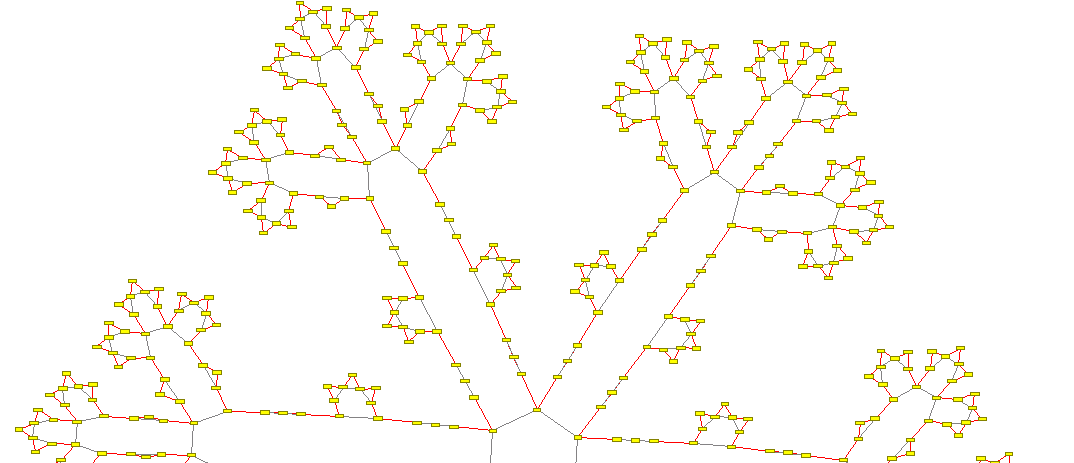
\includegraphics[width=0.9\linewidth]{fig/title}\\[6ex]
  \LARGE Jakob Blomer \qquad Rubino Gei\ss\\ \qquad Edgar Jakumeit\\[3ex]
  \large \today\\

%  \vfill
%	\large Technical Report 2007-5\\
%	\large ISSN 1432-7864

  \setlength{\parindent}{\saveparindent}
\end{titlepage}
\clearpage

\chapter*{Abstract}

\parpic[l] {

\includegraphics[width=45mm]{fig/grgen-256.png}
}

\noindent \textsc{GrGen.NET}: transformation of structures made easy
-- with languages for graph modeling, pattern matching, and rewriting, as well as rule control;
brought to life by a compiler and a rapid prototyping environment offering graphical and step-wise debugging.
The Graph Rewrite Generator is a tool enabling elegant and convenient development of graph rewriting applications with comparable performance to conventionally developed ones.
This user manual contains both, normative statements in the sense of a reference manual as well as an informal guide to the features and usage of \GrG.\\[6ex]

\vspace{13cm}

\parpic[l] {

\includegraphics{fig/by-sa.png}
}
\noindent This manual is licensed under the terms of the \emph{Creative Commons Attribution-Share Alike 3.0 Germany}
license.  The license is available at
\url{http://creativecommons.org/licenses/by-sa/3.0/de/}

\chapter*{Foreword}

Since the last version of this manual which was written for \GrG\ v1.4 a lot has happened, 
as can be seen quite easily in the fact that this manual describes \GrG\ v2.6.
The porting of C to C\# \cite{Kro:07} allowed for a faster pace of development,
which yielded alternatives and subpatterns allowing for structural recursion \cite{Jak:08,StructuralRecursion},
undirected edge support plus fine grain pattern conditions \cite{SABuchwald:2008}, 
a data model that is more user friendly at the API, support for visited flags, 
and an prototypical implementation of an embedding of \GrG\ as s domain specific language into C\# \cite{DAMoritz}
-- resulting in \GrG\ v2.0.
\medskip

Then Dr. Rubino Gei\ss~finished his dissertation \cite{DissRuby} and left; Prof.\ Goos retired.
The succeeding Professor had no commitment to graph rewriting,
so \GrG\ switched from a university project developed by students in their bachelor/masters thesis's
to an open source project (which is still hosted at the IPD, reachable from \url{www.grgen.net}).
\medskip

But development continued:
With the introduction of generic set and map types in the model language to facilitate uses in computer linguistics
and in the rule control language to allow for more concise rule combinations.
With the 2+n pushdown automaton for matching patterns with structural recursion extended 
to handle pattern cardinality specifications and positive applications conditions.
With massive API improvements, now featuring an interface of typed, named entities in addition to the old name string and object based interface.
With the introduction of importers and exporters for GXL (the quasi standard graph exchange format in graph rewriting),
and for GRS, a much easier and less chatty format.\smallskip

Most of these features were introduced due to feedback from users and use cases:\\
We want to thank the organizers of GraBaTs\cite{grabats}, the annual meeting of the graph rewrite tool community,
which gave us the possibility to ruthlessly steal the best ideas of the competing tools.
Thanks to Berthold Hoffmann, for his ``french''-courses and the ideas about how to handle program graphs.
And thanks to several early users giving valuable feedback or even code (\emph{code is of course the best contribution you can give to an open source project}), by name: 
Tom Gelhausen and Bugra Derre (you may have a look at \url{https://svn.ipd.uni-karlsruhe.de/trac/mx/wiki/Home} for some interesting results of this work at IPD Tichy), Paul Bedaride, Normen Müller, and Nicholas Tung.
\\[1ex]

\noindent Regarding questions please contact the \GrG-Team 
via email to \texttt{grgen} at the host given by \texttt{ipd.info.uni-karlsruhe.de}.\\[1ex]

\noindent We hope you enjoy using \GrG\ even more than we enjoyed developing it\\ {\small(it was fun but aging projects with code traces from many people are not always nice to work with ;).}
\\[1ex]

Thank you for using \GrG.\\[2ex]

\noindent Karlsruhe in August 2010, Edgar Jakumeit on behalf of the \GrG-Team

\pagebreak

\chapter*{Foreword for Release 1.4}
First of all a word about the term ``graph rewriting''.
Some would rather say ``graph transformation''; some even think there is a difference between these two.
We don't see such differences and use graph rewriting for consistency.

The \textsc{GrGen} project started in spring 2003 with the diploma thesis of Sebastian Hack under supervision of Rubino Gei\ss.
At that time we needed a tool to find patterns in graph based intermediate representations used in compiler construction.
We imagined a tool that is fast, expressive, and easy to integrate into our compiler infrastructure.
So far Optimix\cite{assmann00graph} was the only tool that brought together the areas of compiler construction and graph rewriting.
However its approach is to feature many provable properties of the system per se, such as termination, confluence of derivations, and complete coverage of graphs.
This is achieved by restricting the expressiveness of the whole formalism below Turing-completeness.
Our tool \textsc{GrGen} in contrast should be Turing-complete.
Thus \GrG\ provides the user with strong expressiveness but leaves the task of proving such properties to the user.

To get a prototype quickly, we delegated the costly task of subgraph matching to a relational database system~\cite{Hac:03}.
Albeit the performance of this implementation could be improved substantially over the years, we believed that there was more to come.
Inspired by the PhD thesis of Heiko D\"orr~\cite{doerr} we reimplemented our tool to use search plan driven graph pattern matching of its own.
This matching algorithm evolved over time~\cite{adam,Bat:05:SA,Bat:05:DA,Bat:06,BKG:07} and has been ported from C to C\#~\cite{KG:07,Kro:07}. 
In the year 2005 Varr\'o~\cite{gramot2005_adapt} independently proposed a similar search plan based approach.

Though we started four years ago to facilitate some compiler construction problems, in the meantime \GrG\ has grown into a general purpose tool for graph rewriting.\\[3ex]

We want to thank all co-workers and students that helped during the design and implementation of \GrG\ as well as the writing of this manual.
Especially we want to thank Dr.~Sebastian Hack, G.~Veit Batz, Michael Beck, Tom Gelhausen, Moritz Kroll, Dr.~Andreas Ludwig, and Dr.~Markus Noga.
Finally, all this would not happened without the productive atmosphere and the generous support that Prof.~Goos provides at his chair.\\[3ex]

We wish all readers of the manual---and especially all users of \GrG---a pleasant graph rewrite experience.
We hope you enjoy using \GrG\ as much as we enjoy developing it.\\[3ex]

Thank you for using \GrG.\\[6ex]

\noindent Karlsruhe in July 2007, Rubino Gei\ss~on behalf of the \GrG-Team




\clearpage

\tableofcontents

\chapter{Introduction}
\label{chp:intro}
\pagenumbering{arabic}


%%%%%%%%%%%%%%%%%%%%%%%%%%%%%%%%%%%%%%%%%%%%%%%%%%%%%%%%%%%%%%%%%%%%%%%%%%%%%%%%%%%%%%%%%%%%%%%%
\section{What Is \GrG?}

{\scshape GrGen} (\textsc{G}raph \textsc{R}ewrite \textsc{Gen}erator) is a generative programming system for graph rewriting,
which considerably eases the \emph{transformation} of \emph{structural} data,
as it is needed e.g. in model transformation, computer linguistics, or modern compiler construction.
\GrG\ is comparable to other programming tools like parser generators which ease the task of formal language recognition,
or databases which ease the task of persistent data storage and querying.


%%%%%%%%%%%%%%%%%%%%%%%%%%%%%%%%%%%%%%%%%%%%%%%%%%%%%%%%%%%%%%%%%%%%%%%%%%%%%%%%%%%%%%%%%%%%%%%%
\section{When to Use \GrG}
You may be interested in using \GrG\ if you have to tackle the task of changing meshes of linked objects, i.e. \emph{graph-like data structures};
anytime the focus is on the \emph{relationship} in between your data entities,
and esp. if your algorithms operate upon data entities that stand in multiple relations to each other.

These tasks are traditionally handled by pointer structures and pointer structure navi\-gation-, search-, and replacement routines written by hand
-- this low-level, pointer-fiddling code can be generated automatically by \GrG\ for you.
You specify your transformation task on a \emph{higher level of abstraction} with nodes connected by edges,
and rewrite rules consisting of \emph{patterns} to be searched as well as modifications to be carried out.
\GrG\ then generates the algorithmic core of your application.
You specify the \emph{what} with \emph{declarative rules}, \GrG\ takes care of the \emph{how};
similar to SQL expressions implemented by database engines, 
or to grammar rules implemented by parser generators.
Development is supported by \emph{visual debugging}, you work on a visualization of your network and the rule applications inside it.
The debugger and the pattern based languages boost your \emph{productivity} for graph-representation-based tasks way beyond traditional programming.
Due to all the optimizations implemented in the pattern matching engine you still gain \emph{high-performance} solutions.
Altogether, \GrG\ offers the highest combined speed of development and execution you can find for those kind of tasks.

%%%%%%%%%%%%%%%%%%%%%%%%%%%%%%%%%%%%%%%%%%%%%%%%%%%%%%%%%%%%%%%%%%%%%%%%%%%%%%%%%%%%%%%%%%%%%%%%
\section{An Example Graph-Based Representation}\label{sub:examplegraphrep}
Let's have a look at an example of a graph-based representation \GrG\ is well suited for 
-- a simplified version of the graph-based compiler intermediate representation \Firm\footnote{\url{www.libfirm.org}} that \textsc{GrGen} was originally developed for.
Nodes represent machine instructions, e.g.\ a \node{Load} fetches a value from an address or an \node{Add} sums two values.
Edges indicate dependencies between nodes, e.g.\ an \node{Add} requires that its two operands are available before it can be executed.
Each instruction is located within a basic block,
all nodes within the \node{Block} are executed if the \node{Block} is executed (in an order allowed by the dependencies).

\begin{figure}[htbp]
	\begin{minipage}[c]{0.43\textwidth}
		\centering
		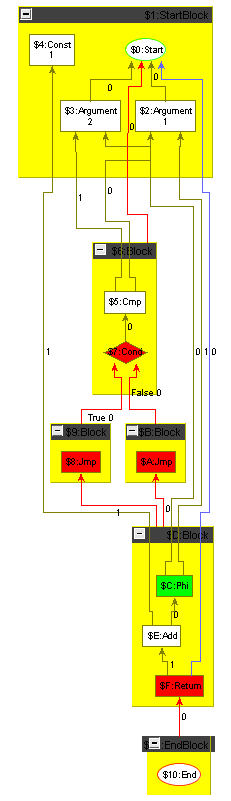
\includegraphics[width=2.3in]{fig/MinPlusNestedArguments.png}
	\end{minipage}
%
	\begin{minipage}[c]{0.57\textwidth}
		\centering
		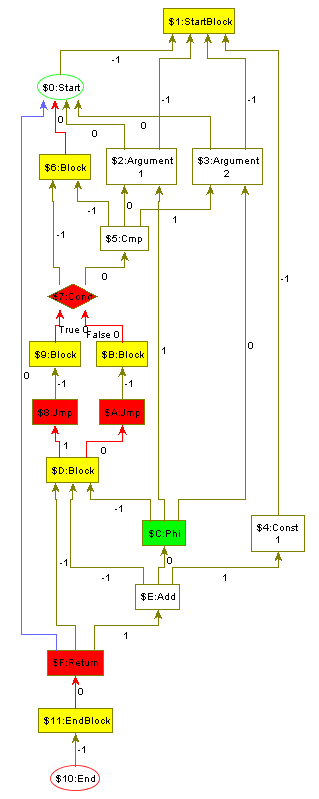
\includegraphics[width=3.3in]{fig/MinPlusPlainArguments.png}
	\end{minipage}
	\caption{Program graph of a minimum plus one function, with block containment visualized as containment left, and the plain graph right.}
	\label{fig:min}
\end{figure}

\autoref{fig:min} shows the program graph for the following C-function:

\pagebreak

\lstinputlisting{resources/MinPlus.c}

Program execution begins at the \node{Start} node, which also produces the initial memory state and the given \node{Argument}s.
The \node{Start} and the \node{Argument}s belong to the special \node{StartBlock}.
The \node{Cmp} compares the arguments, its result is used by the \node{Cond} to carry out a conditional jump depending on the result of the comparison.
After following the \node{Jmp} of the then- or the else-\node{Block}, the program execution is continued at \node{Block} \$D.
The \node{Phi}\footnote{a helper node from the static single assignment form employed; in \cite{braun13cc} you find more information and a simple algorithm for constructing SSA from an abstract syntax tree} 
chooses one of its operands depending on the previously executed block,
here \node{Argument} $1$ if the \node{Cond} was evaluated to \node{True},
or \node{Argument} $2$ if \node{Cond} was evaluated to \node{False}.
The \node{Const}ant 1 is added to the value selected by the \node{Phi},
before the result is returned by the \node{Return}.
The end of the program execution is represented by the special \node{EndBlock} which by convention contains exactly one \node{End}.
If you want to learn more about this representation or typical transformations over it, have a look at the compiler case\cite{CompilerCase} of the TTC 2011 where this representation was used or our solution \cite{CompilerOptimization}.

The key points here are that
\begin{enumerate}
	\item this is a mesh of objects (denoting operations),
	\item that stand to each other in 3 relations (control flow (red), data flow (brown), and memory flow (blue) \footnote{we use dependencies, i.e. the direction is reversed compared to the flow}), 
	\item and a major part of the information is encoded in the connection structure (topology),
	which is explicitly and directly represented with edges.
\end{enumerate}

You find such representations in other domains than \emph{programming languages} and \emph{compilers}, too.
The \emph{knowledge} of an agent about the exterior world can be \emph{represented} intuitively like this with \emph{semantic nets}, you could use \GrG\ for reasoning over them.
\emph{Models} as understood by \emph{model driven engineering} are typically graphs, with \GrG\ you can implement a model transformation between models, or into a lower-level program representation.
When working in \emph{computational linguistics} you may be interested in modeling an \emph{abstract syntax graph} in \GrG;
the recursive and iterated patterns that allow to process tree-like data structures declaratively render \GrG\ an excellent match for such tasks.
But also in \emph{engineering} or \emph{architecture} where you need to describe the buildup of the modeled system from components, here you can derive context-sensitively system \emph{blueprints} or simulate their behaviour.
You find help not only in modelling them, but also in deriving all interesting configurations or simulating all interesting execution traces. 
In form of the built-in support for a backtracking search through a search space or even the enumeration of a state space with isomorphic state pruning, guided by match ordering and filtering.


%%%%%%%%%%%%%%%%%%%%%%%%%%%%%%%%%%%%%%%%%%%%%%%%%%%%%%%%%%%%%%%%%%%%%%%%%%%%%%%%%%%%%%%%%%%%%%%%
\section{When Not to Use \GrG}
There is nothing to gain from \GrG\ if scalars, lists or arrays are sufficient to model your domain,
which is the case for a lot of tasks in computing indeed.
(But which is not the case for others which would be better modeled with trees and especially graphs,
but aren't because of the cost of maintaining pointer structures by hand.)
\GrG\ is likely too heavyweight if you are just interested in computing shortest paths in simple graphs.
You're better off with a traditional graph library and its set of pre-implemented algorithms --
the library can be learned quicker and the algorithms can be reused directly.
\GrG\ with its domain-specific languages in contrast requires some time to learn and some effort to specify or code a solution in.

The graph rewrite generator is not the right tool for you if you're searching for a visual environment to teach children programming -- it's a powerful tool for (software) engineers.
Simpler and less powerful languages like story diagrams\cite{storydiagrams} that can be learned quicker and understood more intuitively may be a better match here.
Neither is it what you need if your graph structured data is to be interactively edited by an end user instead of being automatically transformed by rules (the editor generator DiaGen\cite{diagen} may be of interest in this case).

Each object-oriented program contains a heap of objects pointing to each other that can be understood as a graph like representation, with objects being the nodes and the references being the (fixed) edges.
In contrast to object-oriented programming is the topology in graph-oriented programming as offered by \GrG\ not hidden and encapsulated in the objects, but globally open for inspection and modification;
open and readily accessible for pattern matching and rewriting.
Prefer the closed heaps if you don't need a global view on the data, they are cheaper and the information hiding cuts dependencies.

%If you don't need to map one complete representation to another complete representation,
%or if you don't need to match and rewrite patterns inside a representation,
%you are likely better off with the stronger information hiding of object-oriented programming.
%-- it leads to a better software system architecture.
%A certain level of information hiding is offered with hierarchical graphs as offered by \GrG, though.
%The graph inside an attribute is shielded from the graph containing it.


%%%%%%%%%%%%%%%%%%%%%%%%%%%%%%%%%%%%%%%%%%%%%%%%%%%%%%%%%%%%%%%%%%%%%%%%%%%%%%%%%%%%%%%%%%%%%%%%
\section{What Is Graph Rewriting?}\indexmain{graph rewriting}
\label{ov:whatsallabout}

The notion of graph rewriting as understood by \GrG\ is a method for declaratively specifying ``changes'' to a graph.
This is comparable to the well-known term rewriting.
Normally you use one or more \newterm{graph rewrite rules} to accomplish a certain task.
\GrG\ implements an SPO-based approach (as default).
In the simplest case such a graph rewrite rule consists of a tuple $L \rightarrow R$, whereas $L$---the \newterm{left hand side}\indexmainsee{LHS}{left hand side} of the rule---is called \newterm{pattern graph} and $R$---the \newterm{right hand side}\indexmainsee{RHS}{right hand side} of the rule---is the \newterm{replacement graph}.

\begin{figure}[htbp]
	\centering
  \begin{tikzpicture}
    \begin{scope}[minimum size=0.5cm]
      \tikzstyle{every node}=[draw]
      \node (L)     at (0   ,2.5) {$L$};
      \node (R)     at (7   ,2.5) {$R$};
      \node (mL)    at (0   ,0) {};
      \node (mR)    at (7   ,0) {};
      \node[text width=2cm,text badly ragged,minimum size=1cm] (H)     at (0   ,0) {$H$};
      \node[text width=2cm,text badly ragged,minimum size=1cm] (Hs)    at (7   ,0) {$H'$};
    \end{scope}

    \draw[dotted,->] (L) node[above=0.4cm] {Pattern Graph} -> (mL) node[left,midway]  {Match $m$}   node[below=0.6cm] {Host Graph};
    \draw[dotted,->] (R) node[above=0.4cm] {Rewrite Graph} -> (mR)                              node[below=0.6cm] {Result Graph};

    \pgfsetshortenstart{0.5cm}
    \pgfsetshortenend{0.5cm}
    \draw[thick,->]  (L) -> (R)  node[above,midway] {Preservation Morphism $r$} node[below,midway] {Rule};
    \draw[thick,->]  (H) -> (Hs) node[below,midway] {Rule Application};
  \end{tikzpicture}
  \caption{Basic Idea of Graph Rewriting}
  \label{figrule}
\end{figure}

Moreover we need to identify graph elements (nodes or edges) of $L$ and $R$ for preserving them during rewrite.
This is done by a \newterm{preservation morphism} $r$ mapping elements from $L$ to $R$; the morphism $r$ is injective, but needs to be neither surjective nor total.
Together with a rule name $p$ we have $p : L \xrightarrow{r} R$.

The transformation is done by \newterm{application}\indexmainsee{rule application}{application} of a rule to a \newterm{host graph} $H$.
To do so, we have to find an occurrence of the pattern graph in the host graph.
Mathematically speaking, such a \newterm{match} $m$ is an isomorphism from $L$ to a subgraph of $H$.
This morphism may not be unique, i.e.\ there may be several matches.
Afterwards we change the matched \indexed{spot} $m(L)$ of the host graph, such that it becomes an isomorphic subgraph of the replacement graph $R$.
Elements of $L$ not mapped by $r$ are deleted from $m(L)$ during rewrite.
Elements of $R$ not in the image of $r$ are inserted into $H$, all others (elements that are mapped by $r$) are retained.
The outcome of these steps is the resulting graph $H'$. In symbolic language: $H \xRightarrow{m, p} H'$.


%%%%%%%%%%%%%%%%%%%%%%%%%%%%%%%%%%%%%%%%%%%%%%%%%%%%%%%%%%%%%%%%%%%%%%%%%%%%%%%%%%%%%%%%%%%%%%%%
\section{An Example For Rewriting}\indexmain{example}
\label{ov:example}

We'll have a look at a small example.
Graph elements (nodes and edges) are labeled with an identifier.
If a type is necessary then it is stated after a colon.
We start using a special case to construct our host graph: an \indexed{empty pattern} always produces exactly one\footnote{Because of the uniqueness of the total and totally undefined morphism.} match (independent of the host graph). So we construct an apple by applying
\[
  p_0:
  \begin{array}[c]{c}
    \emptyset
  \end{array}
  \begin{array}[c]{c}
    \longrightarrow
  \end{array}
  \begin{array}[c]{c}
    \begin{tikzpicture}[show background rectangle]
      \tikzstyle{every node}=[circle]
      \node[draw] (n1) at (2.5,5) {};
      \node[draw] (n2) at (2,4)   {};
      \node[draw] (n3) at (0,2)   {};
      \node[draw] (n4) at (2,0)   {};
      \node[draw] (n5) at (4,2)   {};

    	\draw[-latex] (n2) --                                  (n1) node[left,midway]  {$e_1$};
    	\draw[-latex] (n2) .. controls +(-1,1) and +(0,1) ..   (n3) node[left,midway]  {$e_2$};
      \draw[-latex] (n3) .. controls +(0,-1) and +(-1,0) ..  (n4) node[left,midway]  {$e_3$};
    	\draw[-latex] (n4) .. controls +(1,0)  and +(0,-1) ..  (n5) node[right,midway] {$e_4$};
      \draw[-latex] (n5) .. controls +(0,1)  and +(1,1) ..   (n2) node[right,midway] {$e_5$};
    \end{tikzpicture}
  \end{array}
\]
to the empty host graph.
As the result we get an apple as new host graph $H$.
Now we want to rewrite our apple with stem to an apple with a leaflet.
So we apply
\[
  p_1:
  \begin{array}[c]{c}
    \begin{tikzpicture}[show background rectangle]
      \tikzstyle{every node}=[circle,minimum size=0.7cm]
      \node[draw] (a) at (2,5.5)  {a};
      \node[draw] (b) at (2,4)    {b};

    	\draw[-latex] (b) -- (a) node[left,midway]  {$x$};
    \end{tikzpicture}
  \end{array}
  \begin{array}[c]{c}
    \longrightarrow
  \end{array}
  \begin{array}[c]{c}
    \begin{tikzpicture}[show background rectangle]
      \tikzstyle{every node}=[circle,minimum size=0.7cm]
      \node[draw] (c) at (2,5.5)  {c};
      \node[draw] (b) at (2,4)    {b};

    	\draw[-latex] (b) .. controls +(-0.7,+0.7) and +(-0.7,-0.7) .. (c) node[left,midway]   {$y$};
    	\draw[-latex] (b) .. controls +(+0.7,+0.7) and +(+0.7,-0.7) .. (c) node[right,midway]  {$z$};
    \end{tikzpicture}
  \end{array}
\]
to $H$ and get the new host graph $H_1$, something like this:
\[
  \begin{array}[c]{c}
    \begin{tikzpicture}[show background rectangle]
      \tikzstyle{every node}=[circle]
      \node[draw] (n1) at (2.5,5) {};
      \node[draw] (n2) at (2,4)   {};
      \node[draw] (n3) at (0,2)   {};
      \node[draw] (n4) at (2,0)   {};
      \node[draw] (n5) at (4,2)   {};

    	\draw[-latex] (n2) --                                  (n1) node[left,midway]  {$e_1$};
    	\draw[-latex] (n2) .. controls +(-1,1) and +(0,1) ..   (n3) node[left,midway]  {$e_2$};
      \draw[-latex] (n3) .. controls +(0,-1) and +(-1,0) ..  (n4) node[left,midway]  {$e_3$};
    	\draw[-latex] (n4) .. controls +(1,0)  and +(0,-1) ..  (n5) node[right,midway] {$e_4$};
      \draw[-latex] (n5) .. controls +(0,1)  and +(1,1) ..   (n2) node[right,midway] {$e_5$};
    \end{tikzpicture}
  \end{array}
  \begin{array}[c]{c}
    \xRightarrow{\quad p_1 \quad}
  \end{array}
  \begin{array}[c]{c}
    \begin{tikzpicture}[show background rectangle]
      \tikzstyle{every node}=[circle]
      \node[draw] (n1) at (2.5,5) {};
      \node[draw] (n2) at (2,4)   {};
      \node[draw] (n3) at (0,2)   {};
      \node[draw] (n4) at (2,0)   {};
      \node[draw] (n5) at (4,2)   {};
      \node[draw] (n6) at (0,0.5)   {};

    	\draw[-latex] (n2) --                                  (n1) node[left,midway]  {$e_1$};
    	\draw[-latex] (n2) .. controls +(-1,1) and +(0,1) ..   (n3) node[left,midway]  {$e_2$};
      \draw[-latex] (n3) .. controls +(-0.7,-0.7) and +(-0.7,+0.7) .. (n6) node[left,midway]  {$e_6$};
      \draw[-latex] (n3) .. controls +(+0.7,-0.7) and +(+0.7,+0.7) .. (n6) node[right,midway] {$e_7$};
    	\draw[-latex] (n4) .. controls +(1,0)  and +(0,-1) ..  (n5) node[right,midway] {$e_4$};
      \draw[-latex] (n5) .. controls +(0,1)  and +(1,1) ..   (n2) node[right,midway] {$e_5$};
    \end{tikzpicture}
  \end{array}
\]
What happened?
\GrG\ has arbitrarily chosen one match out of the set of possible matches, because $x$ matches edge $e_3$ as well as $e_1$.
A correct solution could make use of edge type information.
We have to change rule $p_0$ to generate the edge $e_1$ with a special type ``stem''.
And this time we will even keep the stem.
So let
\[
  p_2:
  \begin{array}[c]{c}
    \begin{tikzpicture}[show background rectangle]
      \tikzstyle{every node}=[circle,minimum size=0.7cm]
      \node[draw] (a) at (2,5.5)  {a};
      \node[draw] (b) at (2,4)    {b};

    	\draw[-latex] (b) -- (a) node[left,midway]  {$x:\text{stem}$};
    \end{tikzpicture}
  \end{array}
  \begin{array}[c]{c}
    \longrightarrow
  \end{array}
  \begin{array}[c]{c}
    \begin{tikzpicture}[show background rectangle]
      \tikzstyle{every node}=[circle,minimum size=0.7cm]
      \node[draw] (c) at (2,5.5)  {c};
      \node[draw] (b) at (2,4)    {b};
      \node[draw] (a) at (3.5,5.5){a};

    	\draw[-latex] (b) -- (a) node[right,midway]  {$x$};
    	\draw[-latex] (b) .. controls +(-0.7,+0.7) and +(-0.7,-0.7) .. (c) node[left,midway]   {$y$};
    	\draw[-latex] (b) .. controls +(+0.7,+0.7) and +(+0.7,-0.7) .. (c) node[above,midway]  {$z$};
    \end{tikzpicture}
  \end{array}.
\]
If we apply $p_2$ to the modified $H_1$ this leads to
\[
  \begin{array}[c]{c}
    \begin{tikzpicture}[show background rectangle]
      \tikzstyle{every node}=[circle]
      \node[draw] (n1) at (2.5,5) {};
      \node[draw] (n2) at (2,4)   {};
      \node[draw] (n3) at (0,2)   {};
      \node[draw] (n4) at (2,0)   {};
      \node[draw] (n5) at (4,2)   {};

    	\draw[-latex] (n2) --                                  (n1) node[left,pos=0.8]  {$e_1:\text{stem}$};
    	\draw[-latex] (n2) .. controls +(-1,1) and +(0,1) ..   (n3) node[left,midway]  {$e_2$};
      \draw[-latex] (n3) .. controls +(0,-1) and +(-1,0) ..  (n4) node[left,midway]  {$e_3$};
    	\draw[-latex] (n4) .. controls +(1,0)  and +(0,-1) ..  (n5) node[right,midway] {$e_4$};
      \draw[-latex] (n5) .. controls +(0,1)  and +(1,1) ..   (n2) node[right,midway] {$e_5$};
    \end{tikzpicture}
  \end{array}
  \begin{array}[c]{c}
    \xRightarrow{\quad p_2 \quad}
  \end{array}
  \begin{array}[c]{c}
    \begin{tikzpicture}[show background rectangle]
      \tikzstyle{every node}=[circle]
      \node[draw] (n1) at (3,5) {};
      \node[draw] (n2) at (2,4)   {};
      \node[draw] (n3) at (0,2)   {};
      \node[draw] (n4) at (2,0)   {};
      \node[draw] (n5) at (4,2)   {};
      \node[draw] (n6) at (2,5.0)   {};

    	\draw[-latex] (n2) --                                  (n1) node[right,pos=0.6] {$e_1:\text{stem}$};
    	\draw[-latex] (n2) .. controls +(-1,1) and +(0,1) ..   (n3) node[left,midway]  {$e_2$};
      \draw[-latex] (n3) .. controls +(0,-1) and +(-1,0) ..  (n4) node[left,midway]  {$e_3$};
    	\draw[-latex] (n4) .. controls +(1,0)  and +(0,-1) ..  (n5) node[right,midway] {$e_4$};
      \draw[-latex] (n5) .. controls +(0,1)  and +(1,1) ..   (n2) node[right,midway] {$e_5$};
    	\draw[-latex] (n2) .. controls +(-0.3,+0.3) and +(-0.3,-0.3) .. (n6) node[left,midway]   {};
    	\draw[-latex] (n2) .. controls +(+0.3,+0.3) and +(+0.3,-0.3) .. (n6) node[right,midway]  {};
    \end{tikzpicture}
  \end{array}.
\]

%%%%%%%%%%%%%%%%%%%%%%%%%%%%%%%%%%%%%%%%%%%%%%%%%%%%%%%%%%%%%%%%%%%%%%%%%%%%%%%%%%%%%%%%%%%%%%%%
\section{An Example Rule Application on the Representation}

An interesting transformation that can be applied on the compiler intermediate representation introduced in section \ref{sub:examplegraphrep} is constant folding.
\autoref{fig:cmpcondfold} highlights the effect of applying the following example rule by showing the situation before it is applied and afterwards:

\begin{grgen}
rule foldCond {
	cond:Cond -df0:Dataflow-> c0:Const;
	falseBlock:Block -falseEdge:False-> cond;
	trueBlock:Block -trueEdge:True-> cond;
	alternative {
		TrueCond {
			if { c0.value == 1; }
			modify {
				delete(falseEdge);
				-jmpEdge:Controlflow<trueEdge>->;
			}
		}
		FalseCond {
			if { c0.value == 0; }
			modify {
				delete(trueEdge);
				-jmpEdge:Controlflow<falseEdge>->;
			}
		}
	}
	modify {
		delete(df0);
		jmp:Jmp<cond>;
	}
}
\end{grgen}

The rule \texttt{foldCond} is used to replace a conditional jump by an unconditional jump, iff it depends just on a constant value.
To this end, the \texttt{cond} is retyped to \texttt{Jmp},
and the dependency on the constant value \texttt{c0} is \texttt{delete}d.
The syntax \texttt{name:type} declares a node of the given type.
An edge is declared with the same syntax, just inscribed into an edge \texttt{-->} representation.
An \texttt{<original>} suffix denotes retyping, specifying the original element to be retyped.
The pattern matches furtheron the blocks where execution continues: \texttt{trueBlock} and \texttt{falseBlock}.
In the true case (\texttt{if \{ c0.value == 1; \}}), the \texttt{falseEdge} to the \texttt{falseBlock} is deleted and the \texttt{trueEdge} to the \texttt{trueBlock} retyped to a normal \texttt{Controlflow} edge; in the false case, the opposite is carried out.

Here the true case applies as you can see from the value \texttt{1} inscribed in the matched constant \node{\$5}.
The elements from the graph that were bound to the pattern elements are highlighted in light-brown, with their pattern name suffixed in double angles, e.g. the \texttt{cond} was matched to \node{\$7} .
Blocks that become unreachable (without control flow predecessors) are assumed to get deleted in a later step of the transformation,
as are duplicate constants.
The benefits of using \GrG{ }can be already felt from this example, they increase at an accelerating speed as the patterns (and rewrites) grow in size and complexity.

\begin{figure}[htbp]
	\centering
	\subfloat[Before folding the Cond, match highlighted.]{\label{fig:cmpfold}
		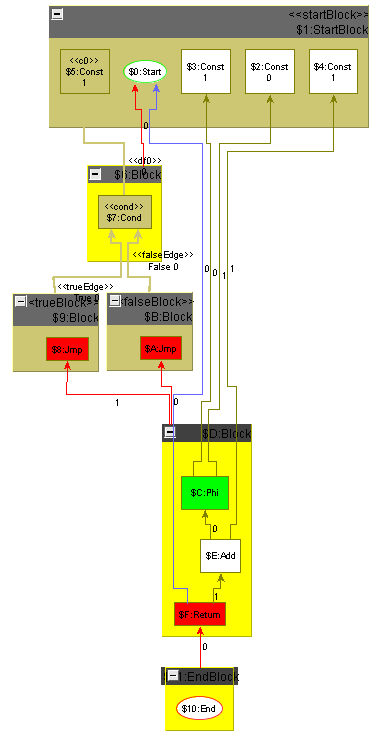
\includegraphics[width=2.89in]{fig/MinPlusCondMatched.png}
	}
	\qquad
	\subfloat[After folding the Cond.]{\label{fig:condfold}
		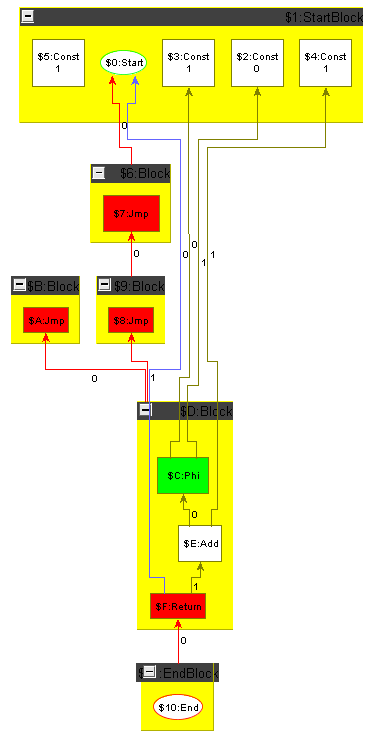
\includegraphics[width=2.7in]{fig/MinPlusCondRewritten.png}
	}
	\caption{Situation reached during folding the program graph of the minimum plus one function when applied to constant arguments.}
	\label{fig:cmpcondfold}
\end{figure}



\chapter{Introduction}
\pagenumbering{arabic}


\section{What is \GrG?}

{\scshape GrGen} (\textsc{G}raph \textsc{R}ewrite \textsc{Gen}erator) is a generative programming system for graph rewriting.
For the potentially expensive matching problem, {\scshape GrGen} applies several novel heuristic optimizations.
According to \indexed{Varr\'o's benchmark}, it is at least one order of magnitude faster than any other tool known to us.

In order to accelerate the matching step, we internally introduce \newterm{search plans} to represent different \newterm{matching strategies} and equip these search plans with a cost model, taking the present host graph into account.
The task of selecting a good search plan is then considered as an optimization problem~\cite{BKG:07,Bat:06}.
For the rewrite step, our tool implements the well-founded \newterm{single-pushout approach} (SPO, for explanation see~\cite{spoapproach}).

For ease of use, {\scshape GrGen} features an expressive specification language and generates program code with a convenient interface.
In contrast to systems like \indexed{Fujaba}~\cite{fujaba} our pattern matching algorithm is fully automatic and does not need to be tuned or partly be implemented by hand.
\GrG~\cite{grgen_web} is the successor of the \textsc{GrGen} tool presented at ICGT 2006~\cite{GBGHS:06}. 
The ``.NET'' postfix of the new name indicates that \textsc{GrGen} has been reimplemented in C\# for the Microsoft .NET or Mono environment~\cite{NET,MONO}.


\section{Features of \GrG}

The process of graph rewriting can be divided into four steps:
Representing a graph according to a model, searching a pattern aka finding a match, performing changes to the matched spot in the host graph, and, finally, selecting the next rule(s) for application.
We have organized the features of \GrG\ according to this breakdown of graph rewriting.

\begin{itemize}
  \item The graph model (meta-model) supports:
  \begin{itemize}
    \item Directed graphs
    \item Typed nodes and edges, with multiple inheritance on types
    \item Node and edge types can be equipped with typed attributes (like structs)
    \item Multigraphs (including multiple edges of the same type)
    \item Connection assertions to restrict the ``shape'' of graphs
  \end{itemize}
  
  \item The pattern language supports:
  \begin{itemize}
    \item Plain isomorphic subgraph matching (injective mapping)
    \item Homomorphic matching for a selectable set of nodes/edges, so that the matching is not injective
    \item Attribute conditions (including arithmetic operations on the attributes)
    \item Type conditions (including powerful instanceof-like type expressions)
    \item Parameter passing to rules
    \item \indexed{Dynamic patterns} with iterative or recursive paths and graphs (yet to be implemented)
  \end{itemize}
  
  \item The rewrite language supports:
  \begin{itemize}
    \item Attribute re-calculation (using arithmetic operations on the attributes)
    \item Retyping of nodes/edges (a stronger version of casts known from common programming languages)
    \item Creation of new nodes/edges of statically as well as dynamically computed types (some kind of generic templates)
    \item Two modes of specification: A rule can either express changes to be made to the match or replace the whole match (the semantics is always mapped to SPO)
    \item Returning certain edges/nodes for further computations
	  \item Copying (duplicating) of elements form the match---comparable with \indexed{sesqui-pushout} rewriting~\cite{CHHK:06} (yet to be implemented)
  \end{itemize}
  
  \item The rule application language (\GrShell) supports:
  \begin{itemize}
    \item Composing several rules with logical and iterative sequence control (called graph rewrite sequences, GRS)
    \item Various methods for creation/deletion/input/output of graphs/nodes/edges 
    \item Stepwise and graphic debugging of rule application
    \item Graph rewrite sequences that can contain nested transactions\indexmain{transaction, nested}
  \end{itemize}
  
  \item Alternatively to \GrShell, you can access the match and rewrite facility through \LibGr. In this way you can build your own algorithmic rule applications in a .NET language of your choice. 
\end{itemize}


\section{System Overview}

Figure~\ref{figsys} gives an overview of the \GrG\ system components. Table~\ref{dirstruc} shows the \GrG\ directory structure.

\begin{figure}[htbp]
  \centering
	\scalebox{0.8}{
  \begin{tikzpicture}
      \begin{scope}[shape=rectangle,minimum size=0.75cm,text width=3cm,text centered]
          \tikzstyle{every node}=[draw]
          \node (spec1)    at (0   ,0)    {Rewrite Rules\indexmain{rewrite rule} (*\indexed{.grg})};
          \node (spec2)    at (0   ,2)    {Graph Model\indexmain{graph model} (*\indexed{.gm})};
          \node (grgen)    at (4   ,1)    {\GrG\ Generator\indexmain{generator} (Java, C\#)};
          \node (rewriter) at (10  ,0)    {Rewrite~Rules (C\#)};
          \node (types)    at (10  ,2)    {Graph~Model (C\#)};
          \node (data)     at (14  ,1)    {Graph~Management (C\#)};
          \node (libgr)    at (12  ,4)    {\LibGr\indexmain{libGr}\ (C\#)};
          \node[fill,color=gray] (app)      at (14.1  ,5.6)  {};
          \node[fill=white] (app)      at (14  ,5.5)  {Applications};
          \node (grsh)     at (10  ,5.5)  {\GrShell\indexmain{GrShell}\ (C\#)};
          \node (grs)      at (6   ,5.5)  {Graph Rewrite Script\indexmain{graph rewrite script}\indexmainsee{GrShell script}{graph rewrite script}\indexmainsee{script}{graph rewrite script} (*\indexed{.grs})};
      \end{scope}

      \node[draw, minimum width=9cm,minimum height=4cm] (engine) at (12,1) {};
      \node[draw, minimum width=9cm,minimum height=4cm,style=dotted] (ct) at (2,1) {};
      \node[anchor=north east] (engine_lab) at (engine.north east) {Backend\indexmain{backend} (Run Time)};
      \node[anchor=north east] (ct_lab) at (ct.north east) {Frontend (Compile Time)};

      \draw[->,dashed,red,>=triangle 45]     (spec1)   -> (grgen);
      \draw[->,dashed,red,>=triangle 45]     (spec2)   -> (grgen);
      \draw[->,dashed,red,>=triangle 45]     (grgen)   -> (types);
      \draw[->,line width=1pt,>=triangle 45] (grgen)   -> (engine);
      \draw[->,dashed,red,>=triangle 45]     (grgen)   -> (rewriter);
      \draw[->,line width=1pt,>=triangle 45] (app)     -> (libgr);
      \draw[->,line width=1pt,>=triangle 45] (grsh)    -> (libgr);
      \draw[->,dashed,red,>=triangle 45]     (grs)     -> (grsh);
      \draw[->,line width=1pt,>=triangle 45] (libgr)   -> (engine);

      \draw[->,line width=1pt,>=triangle 45] (-1.75,5.5) -- +(2.5,0) node[above, midway] {call};
      \draw[->,dashed,red,>=triangle 45] (-1.75,4.5)  -- +(2.5,0) node[above, midway] {read / generate};
  \end{tikzpicture}
	}
  \caption{\GrG\ system components~\cite{Kro:07}}
  \label{figsys}
\end{figure}
\begin{table}[htbp]
  \begin{tabularx}{\linewidth}{|lX|} \hline
  bin & Contains the .NET assemblies, in particular \indexed{GrGen.exe} (the graph rewrite system generator), \indexed{lgspBackend.dll} (a \GrG\ backend), \indexed{LibGr.dll} (the backend API), and the shell \indexed{GrShell.exe}.  \\ 
  lib & Contains the \GrG\ generated assemblies (*.dll). \\
  specs & Contains the graph rewrite system source documents (*.gm and *.grg). \\ \hline
  \end{tabularx}
  \caption{\GrG\ directory structure}
  \label{dirstruc}
\end{table}

A graph rewrite system\footnote{In this context, system is not a CH0-like grammar rewrite system, but rather a set of interacting software components.} is defined by a rule set file (*.grg) and zero or more graph model description files (*.gm). 
Such a graph rewrite system is generated from these specifications by GrGen.exe and can be used by applications such as \GrShell.
Figure~\ref{process} shows the generation process.

\begin{figure}[htbp]
  \centering
	\scalebox{0.8}{
  \begin{tikzpicture}
      \begin{scope}[shape=rectangle,minimum size=0.75cm,text width=3cm,text centered]
          \tikzstyle{every node}=[draw]
          \node (gm1)      at (0   ,0)    {model1.gm};
          \node (gm2)      at (0   ,1)    {model2.gm};
          \node (gm3)      at (0   ,2)    {model3.gm};
          \node (grg)      at (4.5 ,1)    {rules1.grg};
          \node (grgen)    at (10   ,1)    {GrGen.exe};
          \node (act)      at (15.5,1) {rules1Actions.dll};
          \node (backend)  at (10   ,2)    {backend.dll};
          \node (mod)      at (15.5,2)  {rules1Model.dll};
      \end{scope}
         
			\draw[|-|] (-1,-1.5)   -- (5.5, -1.5)    node[below, midway] {/specs};
			\draw[|-|] (9,-1.5)    -- (11, -1.5)     node[below, midway] {/bin};
			\draw[|-|] (14.5,-1.5) -- (16.5, -1.5)   node[below, midway] {/lib};

      \draw[->,line width=1pt,>=triangle 45]     (grg)     -> (gm1);
      \draw[->,line width=1pt,>=triangle 45]     (grg)     -> (gm2);
      \draw[->,line width=1pt,>=triangle 45]     (grg)     -> (gm3);
      \draw[->,dashed,red,>=triangle 45]         (grg)     -> (grgen);
      \draw[->,dashed,red,>=triangle 45]         (grgen)   -> (mod);
      \draw[->,dashed,red,>=triangle 45]         (grgen)   -> (act);
      \draw[->,line width=1pt,>=triangle 45]     (mod)     -> (backend);
      \draw[->,line width=1pt,>=triangle 45]     (act)     -> (backend);


      \draw[->,line width=1pt,>=triangle 45] (-1.25,3.5) -- +(2.5,0) node[above, midway] {referencing};
      \draw[->,dashed,red,>=triangle 45]     (3.25,3.5)  -- +(2.5,0) node[above, midway] {read / generate};
  \end{tikzpicture}
	}
  \caption{Generating a graph rewrite system}
  \label{process}
\end{figure}

In general you have to distinguish carefully between a graph model (meta level), a host graph, a pattern graph and a rewrite rule.
In \GrG\ pattern graphs are implicitly defined by rules, i.e.\ each rule defines its pattern.
On the technical side, specification documents for a graph rewrite system can be available as source documents for graph models and rule sets (plain text *.gm and *.grg files) or as their translated .NET modules, either C\# source files or their compiled assemblies (*.dll).

Generating a \GrG\ graph rewrite system may be considered as preliminary task.
The actual process of rewriting as well as dealing with host graphs is performed by \GrG's backend.
\GrG\ provides a backend \indexed{API}---the .NET library \LibGr.
For most issues---in particular for experimental purposes---you might rather want to work with the \GrShell\ because of its more convenient interface.
However, \GrShell\ does not provide the full power of the \LibGr; see also note~\ref{note:indeterminism} on page~\pageref{note:indeterminism}.

\section{What is Graph Rewriting?}
\label{ov:whatsallabout}

The notion of graph rewriting as understood by \GrG\ is a method for declaratively specifying ``changes'' to a graph.
This is comparable to the well-known term rewriting. 
Normally you use one or more \newterm{graph rewrite rules} to accomplish a certain task.
\GrG\ implements an SPO-based approach.
In the simplest case such a graph rewrite rule consists of a tuple $L \rightarrow R$, whereas $L$---the \newterm{left hand side}\indexmainsee{LHS}{left hand side} of the rule---is called \newterm{pattern graph} and $R$---the \newterm{right hand side}\indexmainsee{RHS}{right hand side} of the rule---is the \newterm{replacement graph}.

\begin{figure}[htbp]
	\centering
  \begin{tikzpicture}
    \begin{scope}[minimum size=0.5cm]
      \tikzstyle{every node}=[draw]
      \node (L)     at (0   ,2.5) {$L$};
      \node (R)     at (7   ,2.5) {$R$};
      \node (mL)    at (0   ,0) {};
      \node (mR)    at (7   ,0) {};
      \node[text width=2cm,text badly ragged,minimum size=1cm] (H)     at (0   ,0) {$H$};
      \node[text width=2cm,text badly ragged,minimum size=1cm] (Hs)    at (7   ,0) {$H'$};
    \end{scope}

    \draw[dotted,->] (L) node[above=0.4cm] {Pattern Graph} -> (mL) node[left,midway]  {Match $m$}   node[below=0.6cm] {Host Graph};
    \draw[dotted,->] (R) node[above=0.4cm] {Rewrite Graph} -> (mR)                              node[below=0.6cm] {Result Graph};

    \pgfsetshortenstart{0.5cm}
    \pgfsetshortenend{0.5cm}
    \draw[thick,->]  (L) -> (R)  node[above,midway] {Preservation Morphism $r$} node[below,midway] {Rule};
    \draw[thick,->]  (H) -> (Hs) node[below,midway] {Rule Application};
  \end{tikzpicture}
  \caption{Basic Idea of Graph Rewriting}
  \label{figrule}
\end{figure}

Moreover we need to identify graph elements (nodes or edges) of $L$ and $R$ for preserving them during rewrite. 
This is done by a \newterm{preservation morphism} $r$ mapping elements from $L$ to $R$; the morphism $r$ is injective, but needs to be neither surjective nor total.
Together with a rule name $p$ we have $p : L \xrightarrow{r} R$.

The transformation is done by \newterm{application}\indexmainsee{rule application}{application} of a rule to a \newterm{host graph} $H$.
To do so, we have to find an occurrence of the pattern graph in the host graph. 
Mathematically speaking, such a \newterm{match} $m$ is an isomorphism from $L$ to a subgraph of $H$.
This morphism may not be unique, i.e.\ there may be several matches.
Afterwards we change the matched \indexed{spot} $m(L)$ of the host graph, such that it becomes an isomorphic subgraph of the replacement graph $R$.
Elements of $L$ not mapped by $r$ are deleted from $m(L)$ during rewrite.
Elements of $R$ not in the image of $r$ are inserted into $H$, all others (elements that are mapped by $r$) are retained.
The outcome of these steps is the resulting graph $H'$. In symbolic language: $H \xRightarrow{m, p} H'$.


\section{An Example}
\label{ov:example}

We'll have a look at a small example. 
Graph elements (nodes and edges) are labeled with and identifier.
If a type is necessary then it is stated after a colon.
We start using a special case to construct our host graph: an \indexed{empty pattern} always produces exactly one\footnote{Because of the uniqueness of the total and totally undefined morphism.} match (independent of the host graph). So we construct an apple by applying
\[
  p_0:  
  \begin{array}[c]{c} 
    \emptyset
  \end{array} 
  \begin{array}[c]{c} 
    \longrightarrow 
  \end{array} 
  \begin{array}[c]{c} 
    \begin{tikzpicture}[show background rectangle]
      \tikzstyle{every node}=[circle]
      \node[draw] (n1) at (2.5,5) {};
      \node[draw] (n2) at (2,4)   {};
      \node[draw] (n3) at (0,2)   {};
      \node[draw] (n4) at (2,0)   {};
      \node[draw] (n5) at (4,2)   {};
    	
    	\draw[-latex] (n2) --                                  (n1) node[left,midway]  {$e_1$};
    	\draw[-latex] (n2) .. controls +(-1,1) and +(0,1) ..   (n3) node[left,midway]  {$e_2$};
      \draw[-latex] (n3) .. controls +(0,-1) and +(-1,0) ..  (n4) node[left,midway]  {$e_3$};
    	\draw[-latex] (n4) .. controls +(1,0)  and +(0,-1) ..  (n5) node[right,midway] {$e_4$};
      \draw[-latex] (n5) .. controls +(0,1)  and +(1,1) ..   (n2) node[right,midway] {$e_5$};
    \end{tikzpicture}
  \end{array}
\]
to the empty host graph. 
As the result we get an apple as new host graph $H$. 
Now we want to rewrite our apple with stem to an apple with a leaflet. 
So we apply
\[
  p_1:
  \begin{array}[c]{c}
    \begin{tikzpicture}[show background rectangle]
      \tikzstyle{every node}=[circle,minimum size=0.7cm]
      \node[draw] (a) at (2,5.5)  {a};
      \node[draw] (b) at (2,4)    {b};
    	
    	\draw[-latex] (b) -- (a) node[left,midway]  {$x$};
    \end{tikzpicture}
  \end{array}
  \begin{array}[c]{c}
    \longrightarrow
  \end{array}
  \begin{array}[c]{c}
    \begin{tikzpicture}[show background rectangle]
      \tikzstyle{every node}=[circle,minimum size=0.7cm]
      \node[draw] (c) at (2,5.5)  {c};
      \node[draw] (b) at (2,4)    {b};
    	
    	\draw[-latex] (b) .. controls +(-0.7,+0.7) and +(-0.7,-0.7) .. (c) node[left,midway]   {$y$};
    	\draw[-latex] (b) .. controls +(+0.7,+0.7) and +(+0.7,-0.7) .. (c) node[right,midway]  {$z$};
    \end{tikzpicture}
  \end{array} 
\]
to $H$ and get the new host graph $H_1$, something like this:
\[
  \begin{array}[c]{c} 
    \begin{tikzpicture}[show background rectangle]
      \tikzstyle{every node}=[circle]
      \node[draw] (n1) at (2.5,5) {};
      \node[draw] (n2) at (2,4)   {};
      \node[draw] (n3) at (0,2)   {};
      \node[draw] (n4) at (2,0)   {};
      \node[draw] (n5) at (4,2)   {};
    	
    	\draw[-latex] (n2) --                                  (n1) node[left,midway]  {$e_1$};
    	\draw[-latex] (n2) .. controls +(-1,1) and +(0,1) ..   (n3) node[left,midway]  {$e_2$};
      \draw[-latex] (n3) .. controls +(0,-1) and +(-1,0) ..  (n4) node[left,midway]  {$e_3$};
    	\draw[-latex] (n4) .. controls +(1,0)  and +(0,-1) ..  (n5) node[right,midway] {$e_4$};
      \draw[-latex] (n5) .. controls +(0,1)  and +(1,1) ..   (n2) node[right,midway] {$e_5$};
    \end{tikzpicture}
  \end{array} 
  \begin{array}[c]{c} 
    \xRightarrow{\quad p_1 \quad}
  \end{array} 
  \begin{array}[c]{c} 
    \begin{tikzpicture}[show background rectangle]
      \tikzstyle{every node}=[circle]
      \node[draw] (n1) at (2.5,5) {};
      \node[draw] (n2) at (2,4)   {};
      \node[draw] (n3) at (0,2)   {};
      \node[draw] (n4) at (2,0)   {};
      \node[draw] (n5) at (4,2)   {};
      \node[draw] (n6) at (0,0.5)   {};
    	
    	\draw[-latex] (n2) --                                  (n1) node[left,midway]  {$e_1$};
    	\draw[-latex] (n2) .. controls +(-1,1) and +(0,1) ..   (n3) node[left,midway]  {$e_2$};
      \draw[-latex] (n3) .. controls +(-0.7,-0.7) and +(-0.7,+0.7) .. (n6) node[left,midway]  {$e_6$};
      \draw[-latex] (n3) .. controls +(+0.7,-0.7) and +(+0.7,+0.7) .. (n6) node[right,midway] {$e_7$};
    	\draw[-latex] (n4) .. controls +(1,0)  and +(0,-1) ..  (n5) node[right,midway] {$e_4$};
      \draw[-latex] (n5) .. controls +(0,1)  and +(1,1) ..   (n2) node[right,midway] {$e_5$};
    \end{tikzpicture}
  \end{array}
\]
What happened? 
\GrG\ has arbitrarily chosen one match out of the set of possible matches, because $x$ matches edge $e_3$ as well as $e_1$.
A correct solution could make use of edge type information. 
We have to change rule $p_0$ to generate the edge $e_1$ with a special type ``stem''.
And this time we will even keep the stem. 
So let
\[
  p_2:
  \begin{array}[c]{c}
    \begin{tikzpicture}[show background rectangle]
      \tikzstyle{every node}=[circle,minimum size=0.7cm]
      \node[draw] (a) at (2,5.5)  {a};
      \node[draw] (b) at (2,4)    {b};
    	
    	\draw[-latex] (b) -- (a) node[left,midway]  {$x:\text{stem}$};
    \end{tikzpicture}
  \end{array}
  \begin{array}[c]{c}
    \longrightarrow
  \end{array}
  \begin{array}[c]{c}
    \begin{tikzpicture}[show background rectangle]
      \tikzstyle{every node}=[circle,minimum size=0.7cm]
      \node[draw] (c) at (2,5.5)  {c};
      \node[draw] (b) at (2,4)    {b};
      \node[draw] (a) at (3.5,5.5){a};
    	
    	\draw[-latex] (b) -- (a) node[right,midway]  {$x$};
    	\draw[-latex] (b) .. controls +(-0.7,+0.7) and +(-0.7,-0.7) .. (c) node[left,midway]   {$y$};
    	\draw[-latex] (b) .. controls +(+0.7,+0.7) and +(+0.7,-0.7) .. (c) node[above,midway]  {$z$};
    \end{tikzpicture}
  \end{array}.
\]
If we apply $p_2$ to the modified $H_1$ this leads to
\[
  \begin{array}[c]{c} 
    \begin{tikzpicture}[show background rectangle]
      \tikzstyle{every node}=[circle]
      \node[draw] (n1) at (2.5,5) {};
      \node[draw] (n2) at (2,4)   {};
      \node[draw] (n3) at (0,2)   {};
      \node[draw] (n4) at (2,0)   {};
      \node[draw] (n5) at (4,2)   {};
    	
    	\draw[-latex] (n2) --                                  (n1) node[left,pos=0.8]  {$e_1:\text{stem}$};
    	\draw[-latex] (n2) .. controls +(-1,1) and +(0,1) ..   (n3) node[left,midway]  {$e_2$};
      \draw[-latex] (n3) .. controls +(0,-1) and +(-1,0) ..  (n4) node[left,midway]  {$e_3$};
    	\draw[-latex] (n4) .. controls +(1,0)  and +(0,-1) ..  (n5) node[right,midway] {$e_4$};
      \draw[-latex] (n5) .. controls +(0,1)  and +(1,1) ..   (n2) node[right,midway] {$e_5$};
    \end{tikzpicture}
  \end{array} 
  \begin{array}[c]{c} 
    \xRightarrow{\quad p_2 \quad}
  \end{array} 
  \begin{array}[c]{c} 
    \begin{tikzpicture}[show background rectangle]
      \tikzstyle{every node}=[circle]
      \node[draw] (n1) at (3,5) {};
      \node[draw] (n2) at (2,4)   {};
      \node[draw] (n3) at (0,2)   {};
      \node[draw] (n4) at (2,0)   {};
      \node[draw] (n5) at (4,2)   {};
      \node[draw] (n6) at (2,5.0)   {};
    	
    	\draw[-latex] (n2) --                                  (n1) node[right,pos=0.6] {$e_1:\text{stem}$};
    	\draw[-latex] (n2) .. controls +(-1,1) and +(0,1) ..   (n3) node[left,midway]  {$e_2$};
      \draw[-latex] (n3) .. controls +(0,-1) and +(-1,0) ..  (n4) node[left,midway]  {$e_3$};
    	\draw[-latex] (n4) .. controls +(1,0)  and +(0,-1) ..  (n5) node[right,midway] {$e_4$};
      \draw[-latex] (n5) .. controls +(0,1)  and +(1,1) ..   (n2) node[right,midway] {$e_5$};
    	\draw[-latex] (n2) .. controls +(-0.3,+0.3) and +(-0.3,-0.3) .. (n6) node[left,midway]   {};
    	\draw[-latex] (n2) .. controls +(+0.3,+0.3) and +(+0.3,-0.3) .. (n6) node[right,midway]  {};
    \end{tikzpicture}
  \end{array}.
\]

\section{The Tools}

All the programs and libraries of \GrG\ are licensed under \indexed{LGPL}. Notice that the \yComp\ graph viewer is not a part of \GrG ; \yComp\ ships with its own license. Although \yComp\ is not free software, it's free for use in academic and non-commercial areas.

\subsection{\texttt{\indexed{GrGen.exe}}}
The \texttt{GrGen.exe} assembly implements the \GrG\ generator. The \GrG\ generator parses a rule set and its model files and compiles them into .NET assemblies. The compiled assemblies interact with the \GrG\ backend.
\begin{description}
  \item[Usage] \texttt{[mono] GrGen.exe [-use <existing-dir>] [-keep] <rule-set> [<output-dir>]}\\
    \emph{rule-set} is a file containing a rule set specification according to chapter~\ref{chaprulelang}. Usually such a file has the suffix \texttt{\indexed{.grg}}. The suffix \texttt{.grg} may be omitted.
By default \GrG\ tries to write the compiled assemblies to the directory \texttt{../lib} relative to the path of \texttt{GrGen.exe}. This can be changed by the optional parameter \emph{output-dir}.
  \item[Options] \mbox{} 
    \begin{tabularx}{\linewidth}{lX}
      \texttt{-keep} & Keep the generated C\# source files. A subdirectory \texttt{tmpgrgen$n$}\footnote{$n$ is an increasing number.} within the current directory will be created. This directory contains:
\begin{itemize}
  \item \texttt{printOutput.txt}---a snapshot of \texttt{stdout} during program execution.
  \item \emph{Name}\texttt{Actions.cs}---the C\# source file of the \emph{rule-set}\texttt{Actions.dll} assembly.
  \item \emph{Name}\texttt{Model.cs}---the C\# source file(s) of the \emph{rule-set}\texttt{Modell.dll} assembly.
\end{itemize}\\
      \texttt{-use} & Don't re-generate C\# source files. Instead use the files in \emph{existing-dir} to build the assemblies.	
    \end{tabularx}
  \item[Requires] .NET 2.0 (or above) or Mono 1.2.2 (or above). Java Runtime Environment 1.5 (or above).
\end{description}

\subsection{\texttt{\indexed{GrShell.exe}}}
The \GrShell\indexmain{GrShell} is a shell application of the \LibGr. \GrShell\ is capable of creating, manipulating, and dumping graphs as well as performing graph rewriting with graphical debug support. For further information about the \GrShell\ language see chapter~\ref{chapgrshell}.

\begin{description}
  \item[Usage] \texttt{[mono] grShell.exe [-c "<commands>" | <grshell-script>]}\\
     Opens the interactive shell. The \GrShell\ will execute the commands in \emph{grshell-script}\indexmain{graph rewrite script} (usually a \texttt{*\indexed{.grs}} file) immediately.  
  \item[Options] \mbox{} 
    \begin{tabularx}{\linewidth}{lX}
      \texttt{-c} & Execute the quoted \GrShell\ commands immediately. Instead of a line break use a double semicolon \texttt{;;} to separate commands.
    \end{tabularx}
  \item[Requires] .NET 2.0 (or above) or Mono 1.2.2 (or above).
\end{description}

\subsection{\texttt{\indexed{LibGr.dll}}}
The \LibGr\indexmain{libGr} is a .NET assembly implementing \GrG's \indexed{API}. See the extracted HTML documentation for interface descriptions. 

\subsection{\texttt{\indexed{yComp.jar}}}
\label{tools:ycomp}
\yComp\indexmain{yComp} \cite{ycomp} is a graph visualization tool based on \yFiles\ \cite{yfiles}. 
It is well integrated in \GrG, but it's not a part of \GrG. \yComp\ implements several graph layout algorithms and has file format support for \indexed{VCG}, GML and YGF among others. 
\begin{description}
  \item[Usage] Usually \yComp\ will be loaded by the \GrShell. You might want to open \yComp\ manually by typing\\
   \texttt{java -jar yComp.jar [<graph-file>]}\\
  The \emph{graph-file} may be any graph file in a supported format. \yComp\ will open this file on startup.
  \item[Hints] Do not use the \indexedsee{compiler graph}{layout algorithm} \indexed{layout algorithm} (\yComp's default setting). 
  Instead \texttt{\indexedsee{Organic}{layout algorithm}} or \texttt{\indexedsee{Orthogonal}{layout algorithm}} might be good choices. 
  Use the rightmost blue play button to start layout process. This may take a while, depending on the graph size:
\begin{center}
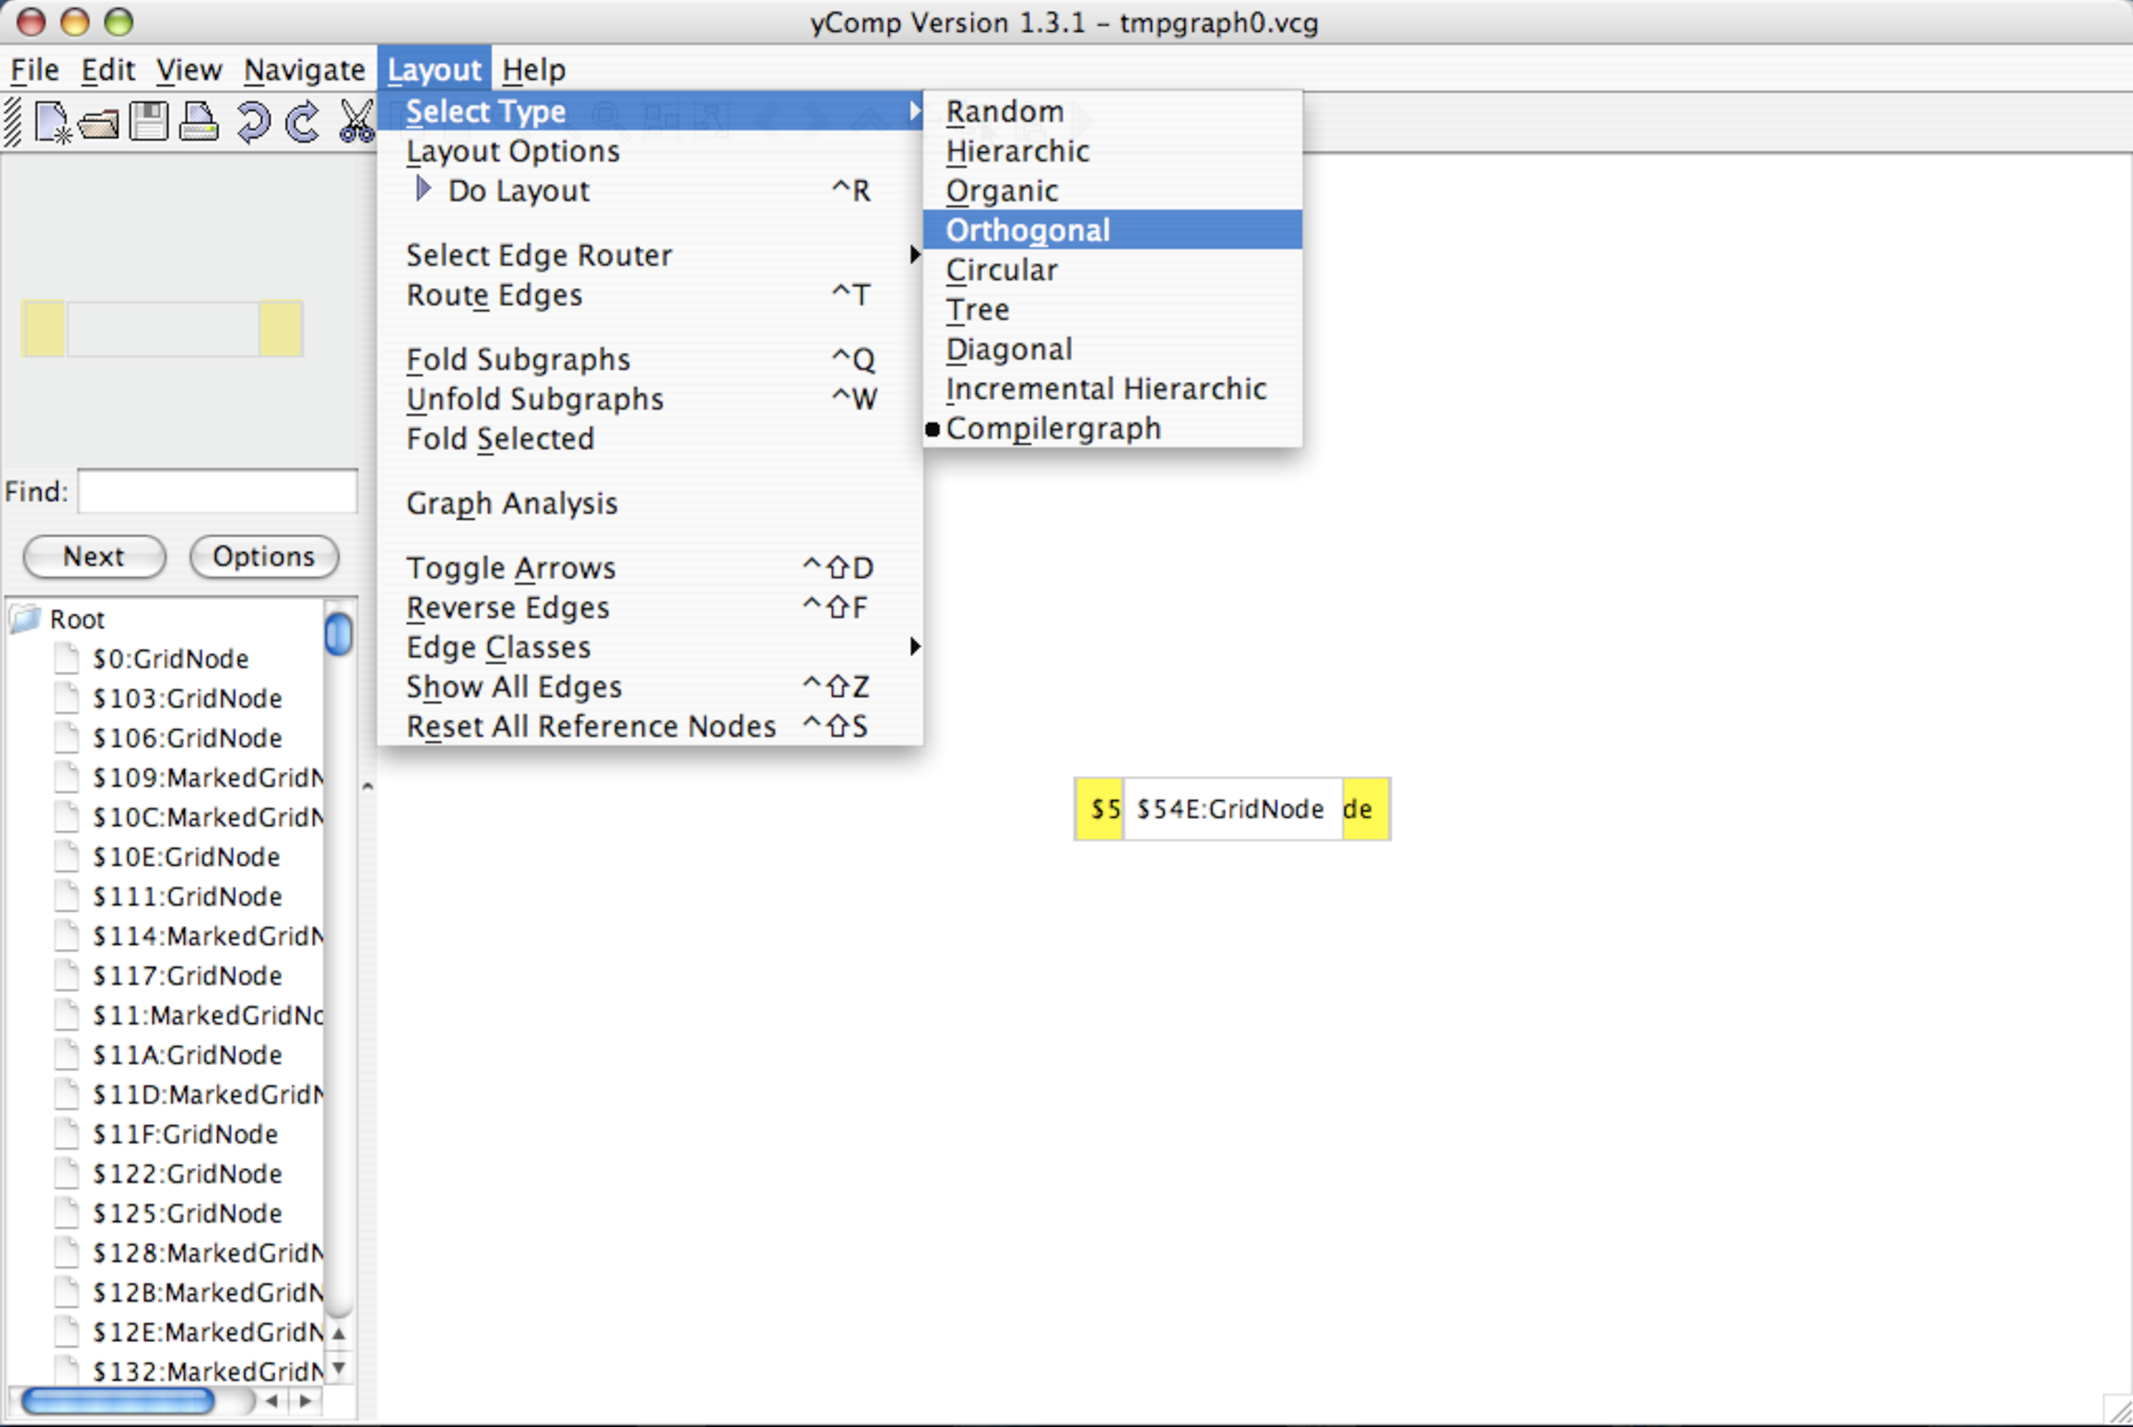
\includegraphics[width=0.45\linewidth]{fig/ycomp1.pdf} 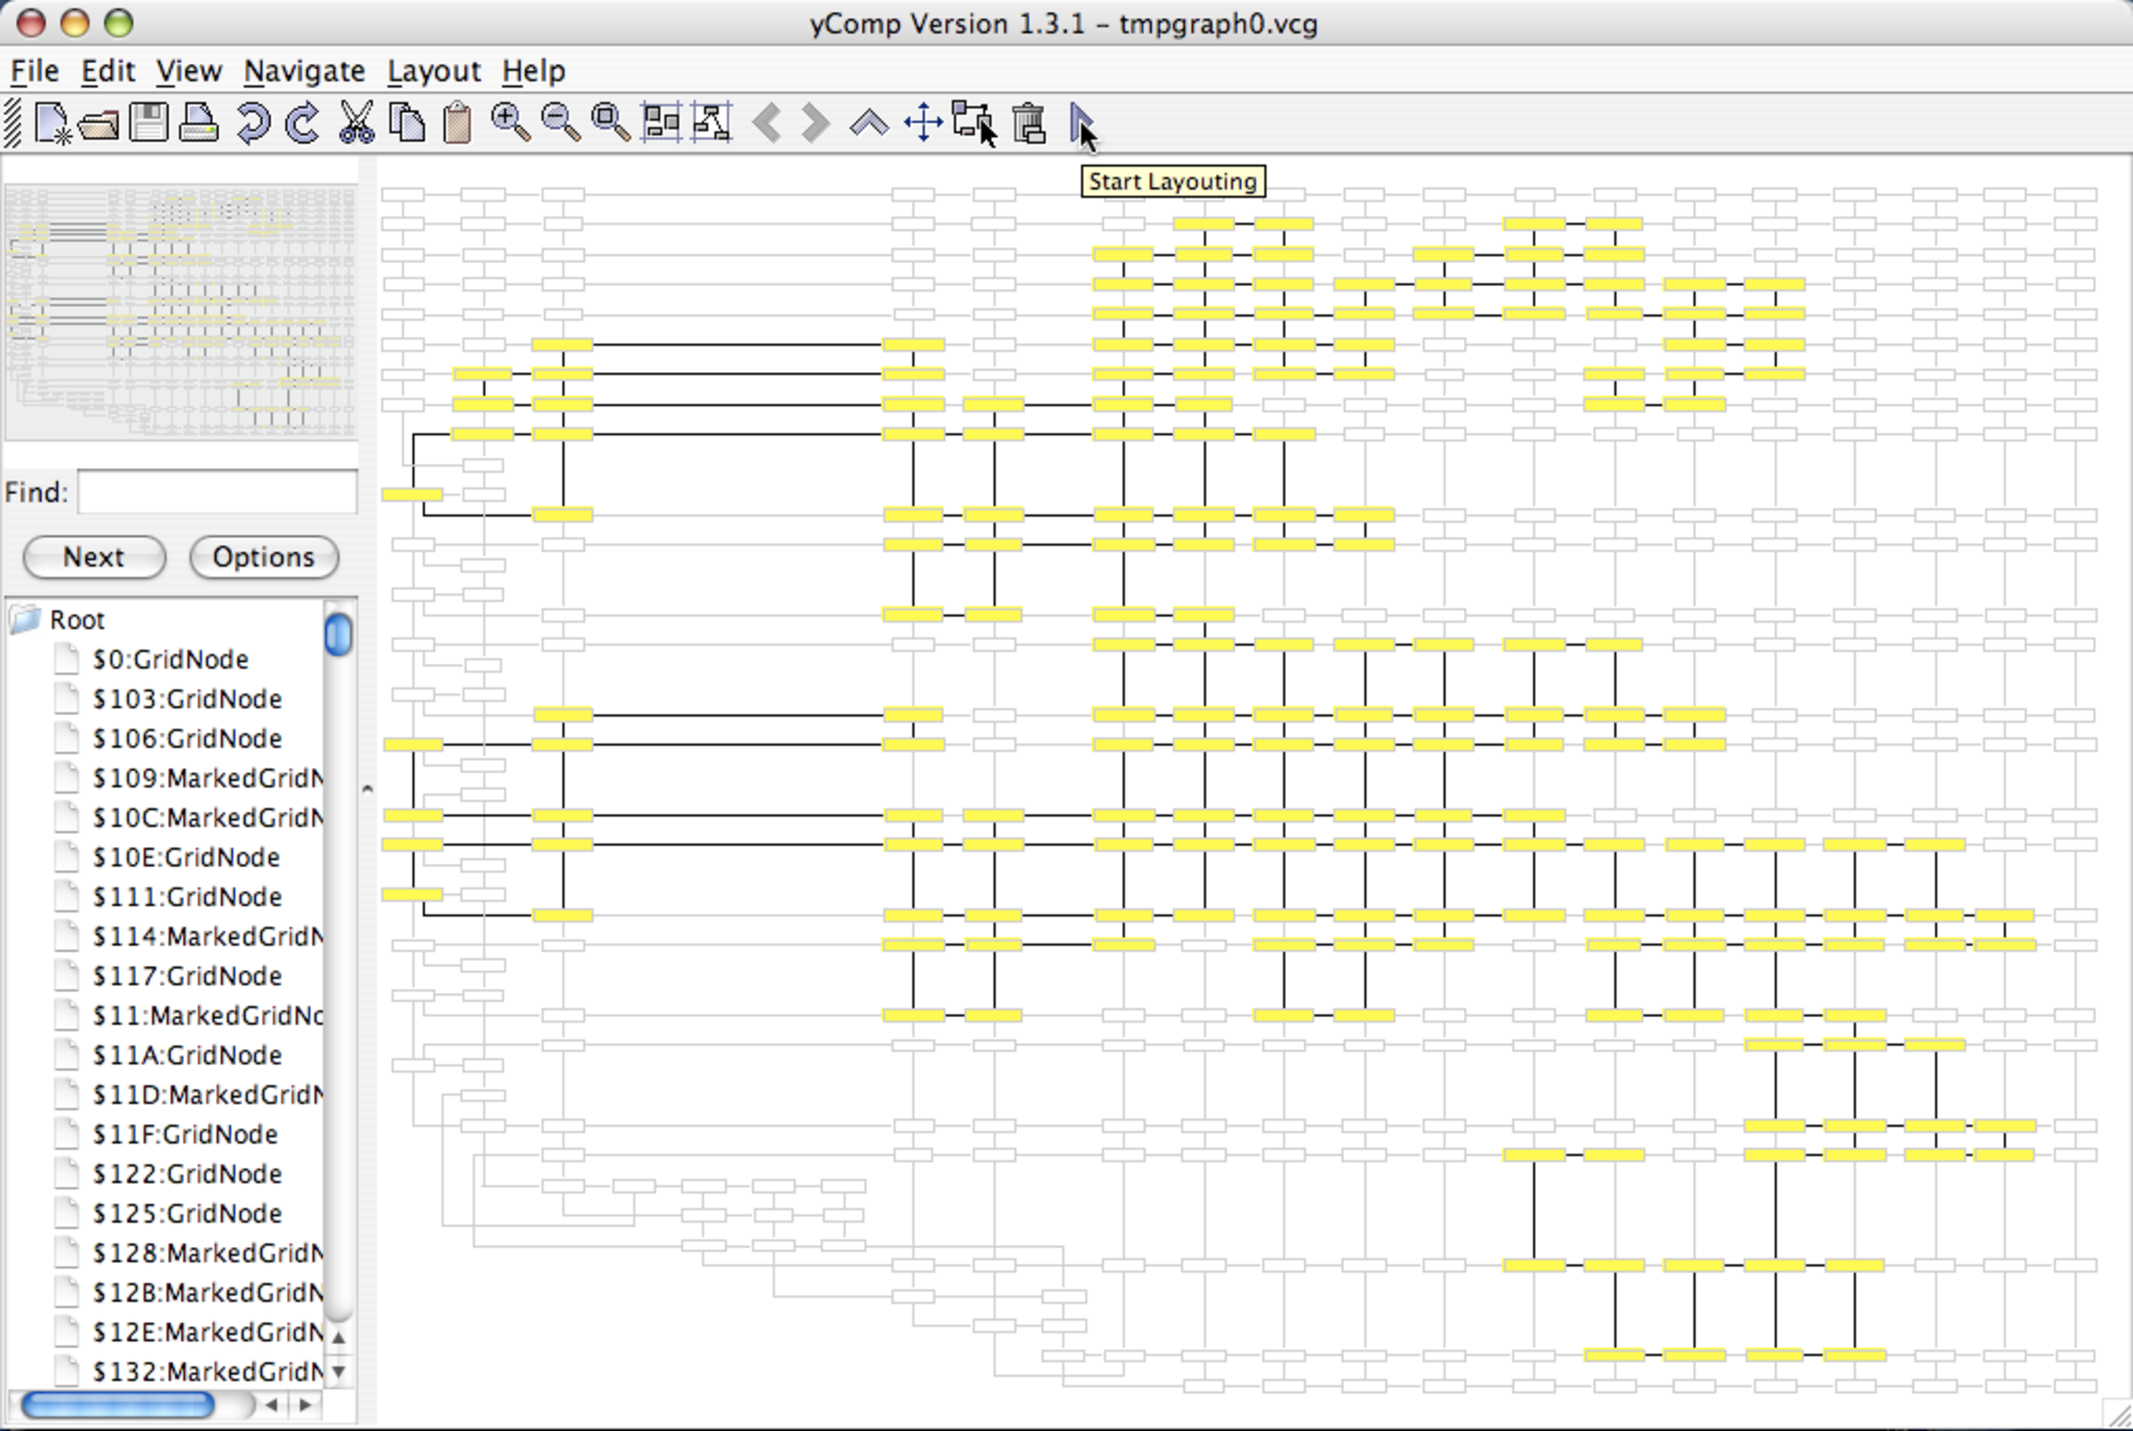
\includegraphics[width=0.45\linewidth]{fig/ycomp2.pdf}
\end{center}
  \item[Requires] Java Runtime Environment 1.5 (or above).
\end{description}




\chapter{Quickstart}\indexmain{quickstart}

In this chapter we'll build a \GrG\ system from scratch. 
You should already have read chapter \ref{chp:intro} to have a glimpse of the \GrG\ system and its components.
We will use \GrG\ to construct non-deterministic state machines.
We further show some actual graph rewriting by removing $\varepsilon$-transitions from our state machines.
This is not too much about details but rather about the \GrG\ look and feel.

\section{Downloading \& Installing}
If you are reading this document, you probably did already download the \GrG\ software from our website (\url{http://www.grgen.net}).
Make sure you have the following system requirements installed
\begin{itemize}
	\item Java 1.5 or above
	\item Mono 1.2.3 on Unix-like platforms / .NET 2.0 or above on Microsoft Windows 
\end{itemize}
Unpack the package to a directory of your choice, for example into \texttt{/opt/grgen} and \texttt{/opt/ycomp}:
\begin{bash}
mkdir /opt/grgen
tar xvfj GrGenNET-V1_3_1-2007-12-06.tar.bz2
mv GrGenNET-V1_3_1-2007-12-06/* /opt/grgen/
rmdir GrGenNET-V1_3_1-2007-12-06
\end{bash}
Add the \texttt{/opt/grgen/bin} directory to your search paths, for instance if you use \texttt{bash} add a line to your \texttt{/home/.profile} file.
\begin{bash}
export PATH=/opt/grgen/bin:$PATH
\end{bash}
Furthermore we create a directory for our \GrG\ data, for instance by \texttt{mkdir /home/grgen}.

\section{Creating a Graph Model}
In the directory \texttt{/home/grgen} we create a text file \texttt{state\_machine.gm} that contains the graph meta model for our state machine.
By graph meta model we mean a set of node types and edge types which are available for building state machine graphs (see chapter \ref{chapmodellang}).
Figure \ref{fig:quick:mm} shows the meta model.
\begin{figure}[htbp]
    \centering
    \begin{grgen}
node class State {
    id: int;
}

abstract node class SpecialState extends State;
node class StartState extends SpecialState;
node class FinalState extends SpecialState;
node class StartFinalState extends StartState, FinalState;

edge class Transition {
    Trigger: string;
}

const edge class EpsilonTransition extends Transition;    
    \end{grgen}
    \caption{Meta Model for State Machines}
    \label{fig:quick:mm}
\end{figure}    
What have we done?
You can see two base types, \texttt{State} for state nodes and \texttt{Transition} for transition edges that will connect the state nodes.
\texttt{State} has an integer attribute \texttt{id} and \texttt{Transition} has a string attribute \texttt{Trigger} which indicates the character sequence for switching from the source state node to the destination state node.
For the rest of the types we use inheritance (keyword \texttt{extends}) which works more or less like inheritance in object oriented languages.
Accordingly the \texttt{abstract} modifier for \texttt{SpecialState} means that you cannot create a node of that precise type, but you might create nodes of non-abstract subtypes.
As you can see \GrG\ supports multiple inheritance and with \texttt{StartFinalState} we have constructed a ``diamond'' type hierarchy.

\section{Creating Graphs}
\label{sct:quick:create}
Let's test our graph meta model by creating a state machine graph.
We will use the \GrShell\ (see chapter chapgrshell) and---for visualization---\yComp.
To get everything working we need a rule set file, too.
For the moment we just create an almost empty file \texttt{remove\_epsilons.grg} in the \texttt{/home/grgen} directory, containing only the line
\begin{grgen}
using state_machine;
\end{grgen}
Now, we could start by launching the \GrShell\ and typing the commands interactively.
This is, however, in most of the cases not the preferred way.
We rather create a \GrShell\ script, say \texttt{remove\_epsilons.grs}, in the \texttt{/home/grgen} directory.
Figure \ref{fig:quick:shell} shows this script.
Run the script by executing \texttt{grshell remove\_epsilons.grs}.
The first time you execute the script, it might take a while because \GrG\ has to compile the meta model and the rule set into .NET assemblies.
\begin{figure}[htbp]
    \centering
    \begin{grgen}
new graph remove_epsilons "StateMachineGraph"

new :StartState($=S, id=0)
new :FinalState($=F, id=3)
new :State($="1", id=1)
new :State($="2", id=2)
new @(S)-:Transition(Trigger="a")-> @("1")
new @("1")-:Transition(Trigger="b")-> @("2")
new @("2")-:Transition(Trigger="c")-> @(F)
new @(S)-:EpsilonTransition-> @("2")
new @("1")-:EpsilonTransition-> @(F)
new @(S)-:EpsilonTransition-> @(F)

show graph ycomp
    \end{grgen}
    \caption{Constructing a state machine graph in \GrShell}
    \label{fig:quick:shell}
\end{figure}
The graph viewer \yComp\ opens and you get a window similiar to figure \ref{fig:quick:ycomp} after clicking the blue ``layout graph'' button on the very right side of the button bar (see also section \ref{tools:ycomp}).
\begin{figure}[htbp]
	\centering
	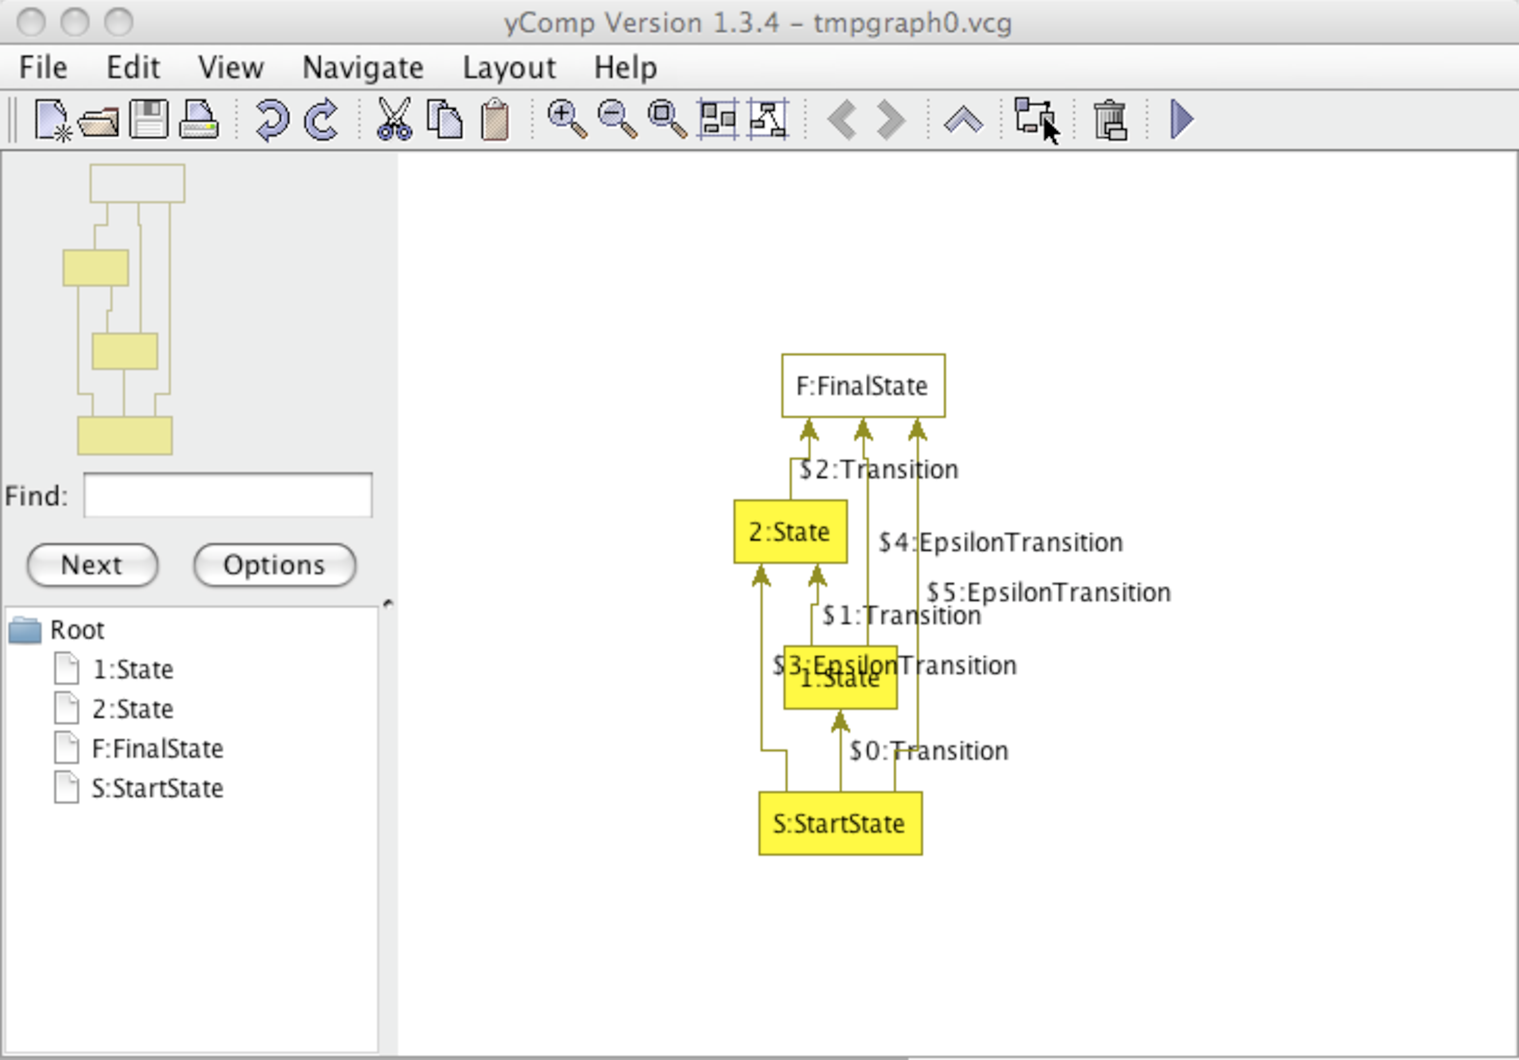
\includegraphics[width=0.8\linewidth]{fig/quickycomp}
	\caption{A first state machine}
	\label{fig:quick:ycomp}
\end{figure}
The graph looks still a bit confusing.
In fact it is quite normal that \yComp's automatic layout algorithm needs manual adjustments.
Quit \yComp\ and exit the \GrShell\ by typing \texttt{exit}.

This script starts with creating an empty graph of the meta model \texttt{StateMachine} (which is referenced by the rule set \texttt{remove\_epsilons.grg}) with the name \texttt{StateMachineGraph}.
Thereafter we create nodes and edges.
The double point notation indicates a node or edge type.
Also note the inplace-arrow notation for edges (\texttt{-Edge->} resp.\ \texttt{-:EdgeType->}).
As you can see, attributes of graph elements can be set during creation with a call-like syntax.
\makeatletter
The \texttt{\$} and \texttt{@} notation is due to the fact that we have two kinds of ``names'' in the \GrShell.
Namely we have \emph{shell variables}---which we did not use, no shell variable is explicitly defined in this script---and \emph{persistent names} that denote a specific graph element.
Persistent names are set by \texttt{\$=Identifier} on creation and accessed by \texttt{@(Identifier)}.
\makeatother
The quote chars around \texttt{"1"} and \texttt{"2"} are used to type these characters as (identifier) strings rather than numbers.

\section{The Rewrite Rules}
We will now add the actual rewrite rules to the rule set file \texttt{remove\_epsilons.grg}.
The idea is to ``forward'' the $\varepsilon$-transitions one after another, i.e.\ if we have a pattern like \texttt{a:State -EpsilonTransition-> b:State -e:Transition-> c:State} we forward to \texttt{a -e-> c}.
After all such transitions are forwarded we can remove the $\varepsilon$-transitions alltogether.
The complete rule set is shown in figure \ref{fig:quick:ruleset}.
See chapter \ref{chaprulelang} for the rule set language reference.
\begin{figure}[htbp]
	\centering
	\begin{grgen}
using state_machine;

test CheckStartState {
    x: StartState;
    negative {
        x;
        y: StartState;
    }
}

test CheckDoublettes {
    negative {
        x:State -e:Transition-> y:State;
        hom(x,y);
        x -doublette:Transition-> y;
        if { typeof(doublette) == typeof(e); }
        if { ((typeof(e) == EpsilonTransition) || (e.Trigger == doublette.Trigger)); }
    }
}

rule ForwardTransition {
    x:State -:EpsilonTransition-> y:State -e:Transition-> z:State;
    hom(x,y,z);
    negative {
        x -exists:Transition-> z;
        if { typeof(exists) == typeof(e); }
        if { ((typeof(e) == EpsilonTransition) || (e.Trigger == exists.Trigger)); }
    }
    modify {
        x -forward:typeof(e)-> z;
        eval { forward.Trigger = e.Trigger; }
    }    
}

rule AddStartFinalState {
    x:StartState -:EpsilonTransition-> :FinalState;
    modify {
        y:StartFinalState<x>;
        emit ("Start state (" + x.id +  ") mutated into a start-and-final state");
    }
}

rule AddFinalState {
    x:State -:EpsilonTransition-> :FinalState;
    if { typeof(x) < SpecialState; }
    modify {
        y:FinalState<x>;
    }
}

rule RemoveEpsilonTransition {
    -:EpsilonTransition->;
    replace {}   
}	
	\end{grgen}
	\caption{Rule set for removing $\varepsilon$-transitions}
	\label{fig:quick:ruleset}
\end{figure}

In detail: The rule set file consists of a number of rules and tests, each of them has a name, like \texttt{ForwardTransition}.
Rules contain a pattern expressed as several semicolon-separated pattern statements and a modify part or a rewrite part.
Tests contain only a pattern; they are used to check for a certain pattern without doing any rewrite operations.
If a rule is applied, \GrG\ tries to find the pattern within a host graph, for instance within the graph we created in section \ref{sct:quick:create}.
Of couse there could be several matches for a pattern---\GrG\ will choose one of them arbitrarily.

Figure \ref{fig:quick:ruleset} also shows the syntax \texttt{x:NodeType} for nodes and \texttt{-e:EdgeType->} for Edges, as we have already seen it in section \ref{sct:quick:create}.
There are also statements like \texttt{:FinalState} or \texttt{-:EpsilonTransistion->}, i.e.\ we are searching for a node of type \texttt{FinalState} resp.\ an edge of type \texttt{EpsilonTransition}, but we are not assigning these graph elements to a name (like \texttt{x} or \texttt{e} above).
Such a defining of names is a key concept of the \GrG\ rule sets: names work as connection points between several pattern statements and between the pattern and the replace / modify part.
As a general rule: If you want to do something with your found graph element, define a name; otherwise an anonymous graph element will do fine.
Also have a look at example \ref{ex:somegraphlets} on page \pageref{ex:somegraphlets} for additional pattern specifications.
The difference between a replace part and a modify part is that a replace part deletes every graph element of the pattern which is not explicitly mentioned in the replace part.
The modify part deletes nothing (by default), but just adds or adjusts graph elements.

What else can we do? 
We have negative application conditions (NACs), expressed by \texttt{negative \{\dots\}}; this prevents a rule to be applicated if the negative pattern is found.
We also have boolean conditions, expressed by \texttt{if \{\dots\}}; a rule is only applicable if all such conditions hold true.
Note, the dot notation to access attributes (as in \texttt{e.Trigger}).
The \texttt{emit} statement prints a string to \texttt{stdout}.
The \texttt{hom(x,y)} and \texttt{hom(x,y,z)} statements mean ``match the embraced nodes homomorphically'', i.e.\ they can actually be matched to the same node within the host graph.
The \texttt{eval \{\dots\}} statement is used to recalculate attributes of graph elements.
Have a look at the statement \texttt{y:StartFinalState<x>} in \texttt{AddStartFinalState}: we \emph{retype} the node \texttt{x}.
That means the newly created node \texttt{y} is actually the node \texttt{x} (including its incident edges and attribute values) except for the node type which is changed to \texttt{StartFinalState}.
Imagine retyping as kind of a type cast.

Now that we have the rules as rewrite primitives we have to compose them to a sequence of rules.
For instance we don't want to forward just one $\varepsilon$-transition as \texttt{ForwardTransition} would do; we want to forward them all.
Such a rule composing is done by a \emph{graph rewrite sequence} (see section \ref{sct:xgrs}).
We add the following line to our shell script \texttt{remove\_epsilons.grs}:
\begin{grgen}
debug xgrs (CheckStartState && CheckDoublettes) && <ForwardTransition* | AddStartFinalState | AddFinalState* | RemoveEpsilonTransition*>
\end{grgen}
This looks like a boolean expression and in fact it behaves similar.
The whole expression is evaluated from left to right.
A rule is successful evaluated if a match could be found.
We first check for a valid state machine, i.e.\ if the host graph has exactly one start state and no redundant transitions.
Thereafter we do the actual rewriting.
These three steps are connected by lazy-evaluation-ands (\texttt{\&\&}), i.e.\ if one of them fails the evaluation will be canceled.
We continue by disjunctive connected rules (connected by \texttt{|}).
The angle brackets (\texttt{<>}) around the transformation rules indicate transactional processing: If the enclosed sequence returns \texttt{false} for some reason, all the already performed graph operations will be rolled back.
That means not all of the rules must find a match.
The \texttt{*} is used to apply the rule repeatedly as long as a match can be found.
This includes applying the rule zero times.
Even in this case \texttt{Rule*} is still successful.

\section{Debugging and Output}
If you execute the modified \GrShell\ script, \GrG\ starts its debugger.
This way you can follow the evaluation of the graph rewrite sequence step by step in \yComp.
Just play around with the keys \texttt{d}, \texttt{s}, and \texttt{r} in \GrShell: the \texttt{d} key lets you follow a single rewrite operation in multiple steps; the \texttt{s} key jumps to the next rule; and the \texttt{r} key runs to the end of the graph rewrite sequence.
Finally you should get a graph like the one in figure \ref{fig:quick:final}
\begin{figure}[htbp]
	\centering
	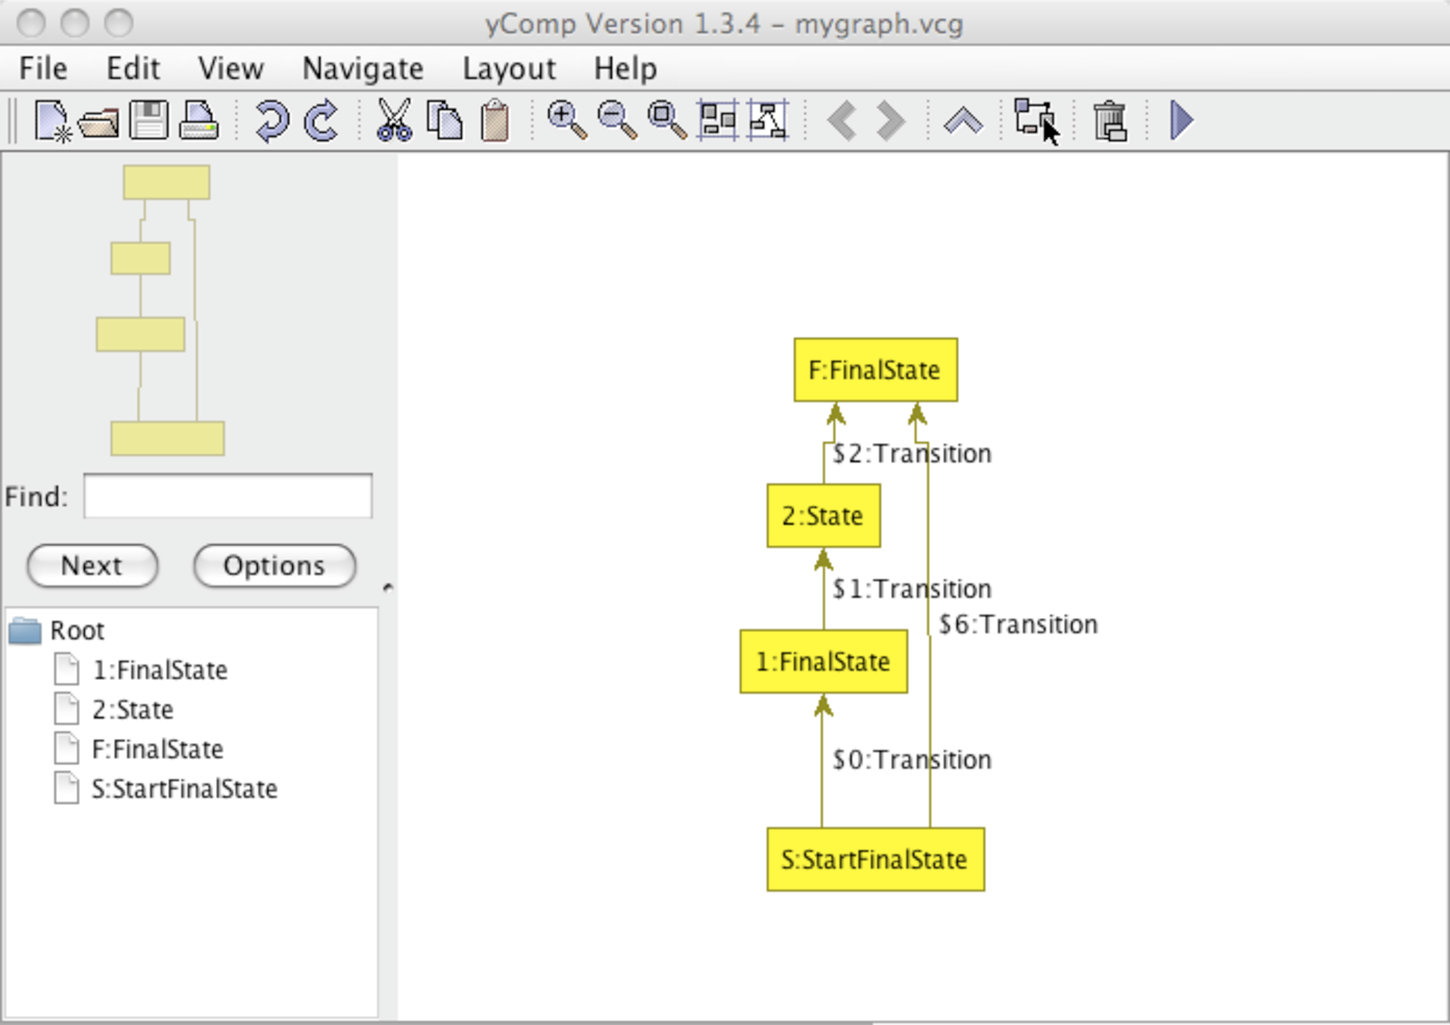
\includegraphics[width=0.8\linewidth]{fig/quickfinal}
	\caption{A state machine without $\varepsilon$-transitions}
	\label{fig:quick:final}
\end{figure}

If everything is working fine you can delete the \texttt{debug} keyword in front of \texttt{xgrs}.
Maybe you want to save the resulting graph.
This is possible by typing \texttt{dump graph mygraph.vcg} in the \GrShell.
\GrShell\ writes the graph in \texttt{mygraph.vcg} into the current directory.
Files in VCG format are readable by \yComp.
Feel free to browse the \texttt{examples} folder shiped with \GrG\ and have a look at further capabilities of the software.


\chapter{Graph Model Language}\indexmain{graph model language}
\label{chapmodellang}
The key features of \GrG\ \emph{graph models}\indexmain{graph model} as described by Geiß et al. \cite{GBGHS:06,KG:07}:

\begin{description}
\item[Types] Nodes and edges are typed. 
  This is similar to classes in common programming languages, except for the concept of methods that \GrG\ nodes and edges don't support. 
\item[Attributes] Nodes and edges can possess attributes. The set of attributes assigned to a node or edge is determined by its type. The attributes themselves are typed, too.
\item[Inheritance] Node and edge types (classes) can be composed by multiple \indexed{inheritance}. \texttt{Node} and \texttt{Edge} are built-in root types of node and edge types, respectively. Inheritance eases the specification of attributes because subtypes inherit the attributes of their super types. Note that \GrG\ lacks a concept of overwriting. On a path in the \indexed{type hierarchy} graph from a type up to the built-in root type there must be exactly one declaration for each attribute identifier. Furthermore if multiple paths from a type up to the built-in root type exist, the declaring types for an attribute identifier must be the same on all such paths.
\item[Connection Assertions] To specify that certain edge types should only connect specific nodes, we include connection assertions. Furthermore the number of outgoing and incoming edges can be constrained.
\end{description}

\begin{figure}[htbf]
\begin{example}\label{ex:model:map}
The following toy example of a model of road maps gives a rough picture of the language:
\begin{grgen}
model Map;

enum resident {village = 500, town = 5000, city = 50000}

node class sight;

node class city {
	size: resident;
}

const node class metropolis extends city {
  river: string;
}  

abstract node class abandoned_city extends city;
node class ghost_town extends abandoned_city;

edge class street;
edge class trail extends street;
edge class highway extends street
    connect metropolis [+] -> metropolis [+]
{
    jam: boolean;
}
\end{grgen}
\end{example}
\end{figure}
In this chapter as well as in chapter \ref{chapgrshell} (\GrShell) we use excerpts of example~\ref{ex:model:map} (the \texttt{Map} model) for illustration purposes.

\section{Building Blocks}
\label{modelbb}

\begin{note}
The following syntax specifications make heavy use of \newtermsee{syntax diagram}{rail diagram}s (also known as \indexed{rail diagram}s). Syntax diagrams provide a visualization of EBNF\footnote{Extended Backus–Naur Form.} grammars. Follow a path along the arrows through a diagram to get a valid sentence (or sub sentence) of the language. Ellipses represent terminals whereas rectangles represent non-terminals. For further information on syntax diagrams see \cite{MMJW:91}.
\end{note}
Basic elements of the \GrG\ graph model language are identifiers to denominate types, attributes, and the model itself. The \GrG\ graph model language is \indexed{case sensitive}.\\
\\
\emph{Ident}, \emph{IdentDecl}\\ \indexmain{identifier}\nopagebreak
A non-empty character sequence of arbitrary length consisting of letters, digits, or underscores. The first character must not be a digit. \emph{Ident} and \emph{IdentDecl} differ in their role: While \emph{IdentDecl} is a \emph{defining} occurrence of an identifier, \emph{Ident} is a \emph{using} occurrence. An \emph{IdentDecl} non-terminal can be annotated\indexmain{annotation}. See \ref{annotations} for annotations of declarations.
\begin{note}
\label{note:modeldecl}
  The \GrG\ model language does not distinguish between \indexed{declaration}s and \indexed{definition}s. More precisely, every declaration is also a definition. For instance, the following C-like pseudo \GrG\ model language code is illegal:
\begin{grgen}
node class t_node;
node class t_node {
  ...
}
\end{grgen}
Using an identifier before defining it is allowed. Every used identifier has to be defined exactly once.
\end{note}
\mbox{ }\\
\emph{NodeType}, \emph{EdgeType}, \emph{EnumType}\\ \nopagebreak
These are (semantic) specializations of \emph{Ident} to restrict an identifier to denote a node type, an edge type, or an enum type, respectively.

\section{Type Declarations}
\begin{rail}
  GraphModel: 'model' IdentDecl ';' (() + TypeDeclaration);
\end{rail}\ixkeyw{model}\ixnterm{GraphModel}
The \indexed{graph model} consists of its name \emph{IdentDecl} and type declarations defining specific node and edge types as well as enums.

\begin{rail}
  TypeDeclaration: EnumDeclaration | ClassDeclaration
\end{rail}\ixnterm{TypeDeclaration}
\emph{ClassDeclaration} defines a node type or an edge type. \emph{EnumDeclaration} defines an enum type for use as attribute of nodes or edges. Like all identifier definitions, types do not need to be declared\indexmain{declaration} before they are used.

\begin{rail}
  EnumDeclaration: 'enum' IdentDecl lbrace ((IdentDecl (() | '=' IntExpr)) + ',') rbrace ;
\end{rail}\ixkeyw{enum}\ixnterm{EnumDeclaration}
Defines an \indexed{enum type}.

\begin{example}
\begin{grgen}
enum Color {red, green, blue}
enum Resident {village = 500, town = 5000, city = 50000}
enum AsInC {a = 2, b, c = 1, d, e = (int)Resident::village + c}
\end{grgen}
The semantics is as in C \cite{Sch:1990:ANSIC}. So, the following holds: $\texttt{red} = 0$, $\texttt{green} = 1$, $\texttt{blue} = 2$, $\texttt{a}=2$, $\texttt{b}=3$, $\texttt{c}=1$, $\texttt{d}=2$, and $\texttt{e}=501$.
\end{example}

\begin{rail}  
  ClassDeclaration: (() | 'abstract') (() | 'const') (NodeClass | EdgeClass);
\end{rail}\ixkeyw{abstract}\ixkeyw{const}\ixnterm{ClassDeclaration}
Defines a new node type or edge type. The keyword \texttt{abstract} indicates that you cannot instantiate graph elements of this type. Instead you have to derive non-abstract types to create graph elements. The abstract-property will not be inherited by subclasses, of course.

\begin{example}
We adjust our map model and make \texttt{city} abstract:
\begin{grgen}
abstract node class city {
	size: int;
}
abstract node class abandoned_city extends city;
node class ghost_town extends abandoned_city;
\end{grgen}
You will be able to create nodes of type \texttt{ghost\_town}, but not of type \texttt{city} or \texttt{abandoned\_city}. However, nodes of type \texttt{ghost\_town} are also of type \texttt{abandoned\_city} as well as of type \texttt{city} and they have the attribute \texttt{size}, hence.
\end{example}
The keyword \texttt{const} indicates that rules may not write to attributes (see also section \ref{replacepart}, \texttt{eval}). However, such attributes are still writable by \LibGr\indexmain{libGr} and \GrShell\indexmain{GrShell} directly. This property applies to attributes defined in the current class, only. It does not apply to inherited attributes. The \texttt{const} property will not be inherited by subclasses, either. If you want a subclass to have the \texttt{const} property, you have to set the \texttt{const} modifier explicitly.

\begin{rail}  
  NodeClass: 'node' 'class' IdentDecl (() | 'extends' (NodeType+',')) \\ 
    (';' | lbrace AttributeDeclarations rbrace);
\end{rail}\ixkeyw{node}\ixkeyw{class}\ixkeyw{extends}\ixnterm{NodeClass}
Defines a new \indexed{node type}. Node types can inherit\indexmain{inheritance} from other node types defined within the same file. If the \texttt{extends} clause is omitted, \emph{NodeType} will inherit from the built-in type \texttt{\indexed{Node}}. Optionally nodes can possess attributes.

\begin{rail}    
  EdgeClass: 'edge' 'class' IdentDecl (() | 'extends' (EdgeType+',')) \\
    (() + ConnectAssertions) (';' | lbrace AttributeDeclarations rbrace);
\end{rail}\ixkeyw{edge}\ixkeyw{class}\ixkeyw{extends}\ixnterm{EdgeClass}
Defines a new \indexed{edge type}. Edge types can inherit\indexmain{inheritance} from other edge types defined within the same file. If the \texttt{extends} clause is omitted, \emph{EdgeType} will inherit from the built-in type \texttt{\indexed{Edge}}. Optionally edges can possess attributes. A \newterm{connection assertion} specifies that certain edge types should only connect specific nodes and, moreover, the number of outgoing and incoming edges can be constrained.

\begin{note}
It is not forbidden to create graphs that are invalid according to \indexed{connection assertion}s. \GrG\ just enables you to check, whether a graph is valid or not. See also section \ref{graphcommands}, \texttt{validate}.
\end{note}

\begin{rail}  
  ConnectAssertions: 'connect' (NodeConstraint '->' NodeConstraint + ',');
  NodeConstraint: NodeType (() | '[' ('*' | '+' | Number | RangeConstraint) ']') ;
  RangeConstraint: Number ':' ('*' | Number) ;
\end{rail}\ixkeyw{connect}\ixnterm{ConnectAssertions}\ixnterm{NodeConstraint}\ixnterm{RangeConstraint}
A \indexed{connection assertion} is denoted as a pair of node types in conjunction with their multiplicities\indexmainsee{multiplicity}{connection assertion}. A corresponding edge may connect a node of the first node type or one of its subtypes (source) with a node of the second node type or one of its subtypes (target). The multiplicity is a constraint on the out-degree and in-degree\indexmainsee{degree}{connection assertion} of the source and target node type, respectively. \emph{Number} is an \texttt{int} constant as defined in section \ref{expressions}. See \ref{graphcommands}, \texttt{validate}\ixkeyw{validate}, for an example. Table \ref{multiplicities} describes the multiplicity definitions.
\begin{table}[htbp]
\begin{tabularx}{\linewidth}{|l|X|}\hline
	\texttt{[$n$:*]} & The number of edges, nodes of that type are incident to, is unbounded. At least $n$ edges must be incident to nodes of that type.\\ 
	\texttt{[$n$:$m$]} & At least $n$ edges must be incident to nodes of that type, but at most $m$ edges may be incident to nodes of that type ($m \geq n$ must hold).\\
	\texttt{[*]} & Abbreviation for \texttt{[0:*]}.\\
	\texttt{[+]} & Abbreviation for \texttt{[1:*]}.\\
	\texttt{[$n$]} & Abbreviation for \texttt{[$n$:$n$]}. \\ \hline
\end{tabularx}
\caption{\GrG\ node constraint multiplicities}
\label{multiplicities}
\end{table}

\begin{rail}    
  AttributeDeclarations: (() | IdentDecl ':' AttributeType ';') + ;
  AttributeType: PrimitiveType | EnumType ; 
\end{rail}\ixnterm{AttributeDeclarations}\ixnterm{AttributeType}
Defines a node or edge \indexed{attribute}. Possible types are enumeration types (\texttt{enum}) and primitive types. See section~\ref{builtin} for a list of built-in primitive types.





\chapter{Rule Set Language}
\label{chaprulelang}

The rule set language forms the core of \GrG. Rule files refer to zero\footnote{Omitting a graph model means that \GrG\ uses a default graph meta model. The default model consists of the base type \texttt{Node} for vertices and the base type \texttt{Edge} for edges.} or more graph models and specify a set of rewrite rules. The rule language covers the pattern specification and the replace/modify specification. Attributes of graph elements can be re-evaluated during a rule application. The following rewrite rule by Geiß et al. \cite{geiss} gives a rough picture of the language:
%\begin{figure}[tb]
\begin{example}\label{ex:rule:SomeRule}
\begin{grgen}
actions SomeActions using SomeModel;

rule SomeRule {
  pattern {
    n1 : NodeTypeA;
    n2 : NodeTypeA;
    hom(n1, n2);
    n1 --> n2; /*@\label{ex:somerule:graphlet}@*/
    n3: NodeTypeB;
    negative {
      n3 -e1:EdgeTypeA-> n1;
      if {n3.a1 == 42*n2.a1;}
    }
    negative { /*@\label{ex:somerule:secondnac:begin}@*/
      n4: Node \ (NodeTypeB);
      n3 -e1:EdgeTypeB-> n4;
      if {typeof(e1) >= EdgeTypeA;}
    } /*@\label{ex:somerule:secondnac:end}@*/
  }
  replace {
    n5: NodeTypeC<n1>;
    n3 -e1:EdgeTypeB-> n5;
    eval {
      n5.a3 = n3.a1*n1.a2;
    }
  }  
}
\end{grgen}
\end{example}
%\end{figure}
In this chapter we use excerpts of example~\ref{ex:rule:SomeRule} (\texttt{SomeRule}) for illustration purposes.

\section{Building Blocks}
\label{rulebb}

The \GrG\ rule set language is case sensitive. The language makes use of several identifier specializations in order to denominate all the \GrG\ entities.\\
\\
\emph{Ident}, \emph{IdentDecl}\\ \nopagebreak
A non-empty character sequence of arbitrary length consisting of letters, digits or underscores. The first character must not be a digit. \emph{Ident} may be an identifier defined in a graph model (see \ref{modelbb}). \emph{Ident} and \emph{IdentDecl} differ in their role: While \emph{IdentDecl} is a \emph{defining} occurrence of an identifier, \emph{Ident} is a \emph{using} occurrence. An \emph{IdentDecl} non-terminal can be annotated. See \ref{annotations} for annotations of declarations.
\begin{note}
  The \GrG\ rule set language does not distinguish between declarations and definitions. More precisely, every declaration is also a definition. That means, that every element of a LHS (left hand side, see section \ref{patternpart}) is actually mapped by a match. 
\end{note}
\mbox{ }\\
\emph{ModelIdent}, \emph{TypeIdent}, \emph{NodeType}, \emph{EdgeType}\\
These are (semantic) specializations of \emph{Ident}. \emph{TypeIdent} matches every type identifier, i.e. a node type, an edge type, an enum type or a primitive type. All the type identifiers are actually type \emph{expressions}. See \ref{typeexpressions} for the use of type expressions.\\

\begin{rail}
  Graphlet: (GraphletNode (() | Continuation) | Continuation) ';' ;
  Continuation: GraphletEdge (() | (GraphletNode (() | Continuation))) ;
\end{rail}
A graphlet specifies a connected subgraph. 
By graphlets \GrG\ provides a descriptive notation to define both, patterns to search for as well as the subgraphs that replace or modify matched spots in a host graph. 
A graph is specified piecewise by graphlets. 
In example \ref{ex:rule:SomeRule}, line \ref{ex:somerule:graphlet}, the statement \texttt{n1 --> n2} is the node identifier \texttt{n1} followed by the continuation graphlet \texttt{--> n2}.

All the graph elements of a graphlet have got a \emph{name}.
The name is either user assigned or an unique internal, non-accessible name.
In the second case the graph element is called \emph{anonymous}.
For illustration purposes we use a \texttt{\$<number>} notation to denote anonymous graph elements in this document.
Names may not be redefined; once defined, a name is \emph{bound} to a graph element. 
We use the term ``binding of names'' because a name not only denote a graph element of a graphlet, but also denotes the mapping of the abstract graph element of a graphlet to a concrete graph element of a host graph.
So graph elements of different names are pairwise distinct except for homomorphically matched graph elements (see section \ref{patternpart}).\\
For instance \texttt{v:NodeType1 -e:EdgeType-> w:NodeType2} selects some node of type \texttt{Node\-Type1} that is connected to a node of type \texttt{NodeType1} by an edge of type \texttt{EdgeType} and binds the names \texttt{v}, \texttt{w}, and \texttt{e}. 
If \texttt{v} and \texttt{w} are not explicitly marked as homomorphic, they are distinct.\\
Binding of names allows for splitting a single graphlet into multiple graphlets as well as defining cyclic structures.
\begin{example}
The following graphlet (\texttt{n1}, \texttt{n2}, and \texttt{n3} are defined somewhere else)
\begin{grgen}
n1 --> n2 --> n3 <-- n1;
\end{grgen}
is equivalent to
\begin{grgen}
n2 --> n3;
n1 --> n2;
n3 <-- n1;
\end{grgen}
and \texttt{n1 --> n3} is equivalent to \texttt{n3 <-- n1}, of course.
\end{example}
The visibility of names is determined by scopes. 
Scopes can be nested. 
Names of surrounding scopes are visible in inner scopes. 
Usually a scope is defined by \texttt{\{} and \texttt{\}}.
In terms of scopes the replace part is a direct inner scope of the pattern part.
In example \ref{ex:rule:SomeRule} the negative condition from lines \ref{ex:somerule:secondnac:begin} to \ref{ex:somerule:secondnac:end} uses \texttt{n3} from the surrounding scope and defines \texttt{n4} and \texttt{e1}. 
We may safely reuse the variable name \texttt{e1} in the replace part.

\begin{rail}
GraphletNode: (Ident | 
    '.' |
    (() | IdentDecl) ':' NodeType (() | TypeConstraint | '<' Ident '>')) ;   
\end{rail}
Specifies a node of type \emph{NodeType} with respect to \emph{TypeConstraint} (see section \ref{typeexpressions}, \emph{TypeConstraint}). 
Type constraints are allowed in the pattern part only. 
The \texttt{.}\ is an anonymous node of the base type \texttt{Node}. 
Remember that every node type has \texttt{Node} as super type. The \texttt{<>} operator retypes a node. Retyping is allowed in the replace/modify part only (see section \ref{replacepart}, \emph{Retyping}).
\begin{center}
  \begin{tabular}[c]{ll}
    \textbf{Graphlet} & \textbf{Meaning}\\ \hline
    \texttt{x:NodeType;} & The name \texttt{x} is bound to a node of type \texttt{NodeType} or one of its subtypes. \\
    \texttt{ :NodeType;} & \texttt{\$1:NodeType} \\
    \texttt{.;} & \texttt{\$1:Node} \\
    \texttt{x;} & The node \texttt{x} is bound to.
  \end{tabular}
\end{center} 

\begin{rail}
  GraphletEdge: '-' (() | EdgeRefinement) '->'  | '<-' (() | EdgeRefinement) '-' ;
  EdgeRefinement: Ident | (() | IdentDecl) ':' EdgeType (() | TypeConstraint | '<' Ident '>') ;
\end{rail}
Specifies an edge. Anonymous edges are specified by \texttt{-->} or \texttt{<--}. For a more detailed specification you can use an inplace notated edge refinement clause. Type constraints are allowed in the pattern part only (see section \ref{typeexpressions}, \emph{TypeConstraint}). The \texttt{<>} operator retypes an edge. Retyping is allowed in the replace/modify part only (see section \ref{replacepart}, \emph{Retyping}).\\
\begin{center}
  \begin{tabular}[c]{ll}
    \textbf{Graphlet} & \textbf{Meaning}\\ \hline
    \texttt{ -e:EdgeType-> ;} & The name \texttt{e} is bound to an edge of type \texttt{EdgeType} or one of its subtypes  \\
    \texttt{ -:EdgeType-> ;} & \texttt{ -\$1:EdgeType-> ;} \\
    \texttt{ --> ;} & \texttt{ -\$1:Edge-> ;} \\
    \texttt{ -e-> ;} & The edge \texttt{e} is bound to.
  \end{tabular}
\end{center} 
As the above table shows, edges can be defined and used separately, i.e.\ without their incident nodes. Beware of accidentally redirecting an edge: 
The graphlets
\begin{grgenlet}
-e:Edge-> .;
x:Node -e-> y:Node;
\end{grgenlet}
are illegal, because they would effect redirecting of edge \texttt{e}. 
However, the graphlets
\begin{grgenlet}
x:Node -e:Edge-> y:Node;
 -e-> ;
\end{grgenlet}
are allowed, but the second graphlet is pointless. In particular the second graphlet does not identify or create any ``copies'', neither occurring in the pattern part nor occurring in the replace part.
\begin{example}
Some attempts to specify a loop edge:\\
\mbox{ }\\
\begin{tabular}[c]{ll} 
 \textbf{Graphlet} & \textbf{Meaning} \\ \hline
 \texttt{x:Node -e:Edge-> x;} & The edge \texttt{e} is a loop.\\ 
 \texttt{x:Node -e:Edge-> ; -e-> x;} & The edge \texttt{e} is a loop.\\ 
 \texttt{-e:Edge-> x:Node;} & The edge \texttt{e} may or may not be a loop.\\ 
 \texttt{.\ -e:Edge-> .;} & The edge \texttt{e} is certainly not a loop.\\ 
\end{tabular}
\end{example}

\begin{figure}[htbp]
\begin{example}
Some graphlets:

\begin{center}
\begin{tabular}[c]{cl}
  & \\
  \begin{tabular}[c]{c}\begin{tikzpicture}
      \tikzstyle{every node}=[circle]
      \node[draw] (n1) at (1,0) {};
      \node[draw] (n2) at (2,1) {};
      \node[draw] (n3) at (1,2) {};
      \node[draw] (n4) at (0,1) {};
    	
      \draw[-latex] (n3) .. controls +(-1,0) .. (n4) {};
      \draw[-latex] (n4) .. controls +(0,-1) .. (n1) {};
      \draw[-latex] (n1) .. controls +(1,0) .. (n2) {};
      \draw[-latex] (n2) .. controls +(0,1) .. (n3) {};
    \end{tikzpicture}\end{tabular} & \begin{tabular}[c]{l} \texttt{x:Node --> .\ --> .\ --> .\ --> x;} \end{tabular}\\
  & \\  
  \begin{tabular}[c]{c}\begin{tikzpicture}
      \tikzstyle{every node}=[circle]
      \node[draw] (n1) at (1,1) {};
      \node[draw] (n2) at (0,0) {};
      \node[draw] (n3) at (0,2) {};
      \node[draw] (n4) at (2,0) {};
      \node[draw] (n5) at (2,2) {};
    	
      \draw[-latex] (n1) -- (n2) {};
      \draw[-latex] (n1) -- (n3) {};
      \draw[-latex] (n1) -- (n4) {};
      \draw[-latex] (n1) -- (n5) {};
    \end{tikzpicture}\end{tabular} & \begin{tabular}[c]{l} \texttt{.\ <-- x:Node --> .;} \\ \texttt{.\ <-- x --> .;} \end{tabular}\\
  & \\
  \begin{tabular}[c]{c}\begin{tikzpicture}
      \tikzstyle{every node}=[circle]
      \node[draw] (n1) at (3,5) {};
      \node[draw] (n2) at (2,4)   {};
      \node[draw] (n3) at (0,2)   {};
      \node[draw] (n4) at (2,0)   {};
      \node[draw] (n5) at (4,2)   {};
      \node[draw] (n6) at (2,5.0)   {};
    	
    	\draw[-latex] (n2) --                                  (n1) node[right,pos=0.6] {$e_1:\text{stem}$};
    	\draw[-latex] (n2) .. controls +(-1,1) and +(0,1) ..   (n3) node[left,midway]  {$e_2$};
      \draw[-latex] (n3) .. controls +(0,-1) and +(-1,0) ..  (n4) node[left,midway]  {$e_3$};
    	\draw[-latex] (n4) .. controls +(1,0)  and +(0,-1) ..  (n5) node[right,midway] {$e_4$};
      \draw[-latex] (n5) .. controls +(0,1)  and +(1,1) ..   (n2) node[right,midway] {$e_5$};
    	\draw[-latex] (n2) .. controls +(-0.3,+0.3) and +(-0.3,-0.3) .. (n6) node[left,midway]   {};
    	\draw[-latex] (n2) .. controls +(+0.3,+0.3) and +(+0.3,-0.3) .. (n6) node[right,midway]  {};
    \end{tikzpicture}\end{tabular} & \begin{tabular}[c]{l} \texttt{.\ <-e1:stem- n1:Node -e2:Edge-> .\ -e3:Edge-> .} \\ \quad\texttt{-e4:Edge-> .\ -e5:Edge-> n1;}\\ \texttt{n1 --> n2:Node;} \\ \texttt{n1 --> n2;} \end{tabular}\\
   & \\
  \begin{tabular}[c]{c}\begin{tikzpicture}
      \tikzstyle{every node}=[circle]
      \node[draw] (n1) at (0,0) {};
      \node[draw] (n2) at (1,0) {};
      \node[draw] (n3) at (2,0) {};
      \node[draw] (n4) at (3,0) {};
      \node[draw] (n5) at (4,0) {};
    	
      \draw[-latex] (n1) -- (n2) {};
      \draw[-latex] (n3) -- (n2) {};
      \draw[-latex] (n4) -- (n3) {};
      \draw[-latex] (n4) -- (n5) {};
    \end{tikzpicture}\end{tabular} & \begin{tabular}[c]{l} \texttt{.\ --> .\ <-- .\ <-- .\ --> .;} \end{tabular}
\end{tabular}\\
\end{center}
\mbox{ }\\
\mbox{ }\\
\mbox{ }\\
And some illegal graphlets:\\
\mbox{}\\
\mbox{}\\
\begin{tabularx}{\linewidth}{cX}
\texttt{-e:Edge-> ; .\ -e-> .;} & Would effect redirecting of edge \texttt{e}. \\
 & \\
 \texttt{x -e:T-> y; x -e-> x;} & Would effect redirecting of edge \texttt{e}. \\
  & \\
 \texttt{x:Node; negative \{y:Node; hom(x,y)\}} & Here \texttt{x} must not occur in the \texttt{hom} statement. See section \ref{patternpart} for further information. \\
  & \\
  \texttt{<-- --> ;} & There must be at least a node between the edges.
\end{tabularx}
\end{example}
\end{figure}

\begin{note}
Although both, the pattern part and the replace/modify part, use graphlets, there are subtle differences between them. It concerns the \emph{TypeConstraint} clause, the retype operator \texttt{<>}, and the scope of defined graph element names: Names defined within the pattern part are valid in the pattern part as well as in the replace/modify part. Names defined within the replace/modify part are unknown to the pattern part.
\end{note}

\section{Rules and Tests}
\label{ruledecls}
The structure of a rule set file is as follows:
\begin{rail}
  'actions' IdentDecl (() | 'using' ((ModelIdent)+',')) ';' \\ ((TestDeclaration | RuleDeclaration)+) ;
\end{rail}
A rule set consists of the underlying graph models and several rewrite rules. In case of multiple graph models \GrG\ uses the union of these models. In this case beware of conflicting declarations. There is no built-in conflict resolution mechanism like packages or namespaces for models. If necessary you could use prefixes as you might do it in C.

\begin{rail}
  TestDeclaration: 'test' ActionSignature lbrace Pattern rbrace ;
  RuleDeclaration: 'rule' ActionSignature lbrace Pattern Replace rbrace ;
\end{rail}
Declares a single rewrite rule such as \texttt{SomeRule}. It consists of a pattern part (see \ref{patternpart}) in conjunction with its rewrite/modify part (see \ref{replacepart}). A \emph{test} has no rewrite specification. It's intended to check whether (and maybe how many times) a pattern occurs.
\begin{example}
We define a test \texttt{SomeCond}
\begin{grgen}
test SomeCond {
  pattern {
    n: SeldomNodeType;
  }
}
\end{grgen}
and execute in \GrShell:
\begin{grshell}
  grs SomeCond & SomeRule
\end{grshell}
SomeRule will only be executed, if a node of type \texttt{SeldomNodeType} exists. For regular graph rewrite sequences in \GrShell\ see \ref{grsthings}.
\end{example}

\begin{rail}  
  ActionSignature: IdentDecl (() | Parameters) (() | ':' ReturnTypes) ;
\end{rail}
The signature sets the name of a rewrite rule to \emph{IdentDecl} and optionally names and types of formal parameters as well as a list of return types. Parameters provide users with the ability to pass graph elements to and from a rule. This is similar to parameters of procedural languages.

\begin{rail}
  Parameters: '(' ((IdentDecl ':' NodeType | '-' IdentDecl ':' EdgeType '->') + ',') ')' ;
  ReturnTypes: '(' ((NodeType | EdgeType) + ',') ')' ;
\end{rail}
Within a rule parameters are treated as (predefined) graph elements of the pattern. Even if a supplied parameter value is undefined, it is treated as valid node or edge definition. So in any case a graph element of the specified type has to be mapped. \GrG\ assumes the lookup operation for parameters to be in $\mathcal{O}(1)$. In case of an undefined parameter value this might lead to bad search plans, because \GrG\ has to actually search for such a graph element.
\begin{example}
Assume the following rule:
\begin{grgen}
rule r(-e:Edge->; x:Node) {
  pattern {
    x --> ;
    negative {
      <-- x -->;
    }
  }
  modify {}
}
\end{grgen}
If \texttt{x} and \texttt{e} are undefined, rule \texttt{r} is equivalent to rule \texttt{s}:
\begin{grgen}
rule s {
  pattern {
    x:Node --> ;
    -e:Edge-> ;
    negative {
      <-- x -->;
    }
  }
  modify {}
}
\end{grgen}
In particular \texttt{x} will not be incident to \texttt{e}.
\end{example}
The return types specify edge and node types of graph elements that are returned by the replace/modify part. If return types are specified, the \texttt{return} statement is mandatory. Otherwise no \texttt{return} statement must occur. See also section \ref{replacepart}, \texttt{return}.
\begin{example}
We extend \texttt{SomeRule} with a variable node to find and we want it to return the rewritten graph elements \texttt{n5} and \texttt{e1}.
\begin{grgen}
  rule SomeRuleExt(varnode: Node): (Node, EdgeTypeB) {
    pattern {
      n1: NodeTypeA;
      ...
    }
    replace {
      varnode;
      ...  
      return(n5, e1);
      eval {
        ...
\end{grgen}
We don't define \texttt{varnode} within the pattern part because this is already covered by the parameter specification itself.
\end{example}

\section{Pattern Part}
\label{patternpart}
\begin{rail}
  Pattern: 'pattern' lbrace (()+PatternStatement) rbrace ;
\end{rail}
A pattern consists of zero or more pattern statements. All the pattern statements must be fulfilled by a subgraph of the host graph in order to form a match. Even stronger -- a graph element of the host graph, that is matched by a statement, is \emph{bound}, i.e.\ it cannot be part of another pattern statement, unless you use the \texttt{hom} operator. An empty pattern always produces exactly one (empty) match. This is caused by the uniqueness of the totally undefined function.\\
Pattern statements may define names for graph elements for use by other pattern statements or replace statements. Such names may be used before their declaration. See section \ref{rulebb} for a detailed explanation of names and graphlets.
\begin{note}
The application of a rule is not deterministic (remember the introducing example in \ref{ov:example}), in particular there may be more than one subgraph that matches the pattern. 
Whereas the \GrShell\ selects one of them arbitrarily (without further abilities to control the selection), the underlying \LibGr\ provides a mechanism to deal with such ambiguities. 
\LibGr\ allows for splitting a rule application into two steps: Find all the subgraphs of the host graph that matches the pattern and rewrite one of this matches. 
By returning a collection of all matches, the \LibGr\ retains the complete graph rewrite process under control.
As a \LibGr\ user use the following methods of the \texttt{IAction} interface:
\begin{csharplet}
IMatches Match(IGraph graph, int maxMatches, IGraphElement[] parameters);
IGraphElement[] Modify(IGraph graph, IMatch match);
\end{csharplet}
This might look like this in C\#:
\begin{csharplet}
IMatches myMatches = myAction.Match(myGraph, -1, null); /* -1: get all the matches */
for (int i = 0;  i < myMatches.NumMatches; i++)
{
	if (inspectCarefully(myMatches.GetMatch(i))
	{
		myAction.Modify(myGraph, myMatches.GetMatch(i));
		break;
  	}
}
\end{csharplet}

Also notice that the regular graph rewrite sequences introduces a further variant of indeterminism on rule application level: 
The \texttt{\$<op>} flag marks the operator \texttt{<op>} as commutative, i.e.\ the execution order of its operands (rules) is indeterministic. 
See section \ref{grsthings} for further information on regular graph rewrite sequences.
\end{note}

\begin{rail}  
  PatternStatement: 
    Graphlet ';' |
    'hom' '(' (Ident + ',') ')' ';' |
    'negative' lbrace (()+PatternStatement) rbrace |
    'if' lbrace (BooleanExpr ';' +) rbrace |
    'return' '(' (Ident+',') ')' ';' ;
\end{rail}
The semantics of the various pattern statements:
\begin{description}
  \item[Graphlet.] Graphlets specify connected subgraphs. See section \ref{rulebb} for a detailed explanation of graphlets. 
  \item[Isomorphic/Homomorphic Matching.] The \texttt{hom} operator specifies the nodes or edges that may be matched homomorphically. In contrast to the default isomorphic matching, the specified graph elements \emph{may} be mapped to the same graph element in the host graph. Note that the graph elements shall have a common supertype. Several homomorphically matched graph elements will be mapped to a graph element of a common supertype.\\
  In example \ref{ex:rule:SomeRule} node \texttt{n1} and node \texttt{n2} may be the same node. This is possible because they are of the same type (\texttt{NodeTypeA}).\\
  The \texttt{hom} operator is transitive, i.e.\ \texttt{hom(a, b); hom(b, c);} implies \texttt{hom(a, c);}. 
  Inside a NAC the \texttt{hom} operator may only operate on graph elements that are either defined or used in the NAC.
  \item[Negative Application Conditions (NACs).] With negative application conditions (keyword \texttt{negative}) we can specify graph patterns which forbid the application of a rule if any of them is present in the host graph (cf. \cite{adam}). 
  NACs must not be nested.
  NACs possess an own scope. 
  Names defined within a NAC are not alive outside the NAC. 
  Identifiers from surrounding scopes may be overwritten.
  In general NACs does not care about bindings within the outer scope. 
  Nevertheless, if you use an identifier that is defined in the outer scope, this specifies exactly the graph element, the identifier is bound to in the outer scope.
  \begin{example}
    We specify a node \texttt{x} with out-degree 2:
    \begin{grgen}
pattern {
  <-- x:Node -->;
  negative {
    <-- x -->;
    x -->;
  }
}
    \end{grgen}
  \end{example}
  \item[Attribute Conditions.] The Java-like attribute conditions (keyword \texttt{if}) in the pattern part allow for further restriction of the applicability of a rule.
  \item[Return values.] The return statement is only allowed for tests. Otherwise the \texttt{return} statement belongs to the replace part. See \ref{replacepart}, \emph{Return Values}.
\end{description}
Keep in mind that using type constraints or the \texttt{typeof} operator might be helpful. See section \ref{typeexpressions} for further information.

\section{Replace/Modify Part}
\label{replacepart}
For the task of rewriting \GrG\ provides two different modes: A replace mode and a modify mode.
\begin{description}
  \item[Replace mode.] The semantics of this mode is to delete every graph element of the pattern that is not used (denoted) in the replace part, keep every graph element that is used, and create every additionally defined graph elements. ``Using'' means using a graph element in a graphlet. Attribute calculations are no using occurrences.\\
  In example \ref{ex:rule:SomeRule} \texttt{SomeRuleExt} the nodes \texttt{varnode} and \texttt{n3} will be kept. The node \texttt{n1} is replaced by the node \texttt{n5} preserving \texttt{n1}'s edges. The anonymous edge instance between \texttt{n1} and \texttt{n2} only occurs in the pattern and therefore gets deleted.
  \item[Modify mode.] The modify mode can be regarded as a replace part in replace mode, where every pattern graph element is added (denoted) before the first replace statement. In particular even the anonymous graph elements are kept. Additionally this mode supports the \texttt{delete} operator that deletes every element given as an argument. Deletion takes place after all other rewrite operations. Multiple deletion of the same graph element is allowed (but pointless) as well as deletion of just created elements (pointless, too).
\begin{example}
How might example \ref{ex:rule:SomeRule} look in modify mode? We have to denominate the anonymous edge between \texttt{n1} and \texttt{n2} in order to delete it. The node \texttt{varnode} should be omitted. So we have
\begin{grgen}
rule SomeRuleModify {
  pattern {
    ...
    n1 -e0:Edge-> n2;
    ...
  }
  modify {
    n5 : NodeTypeC<n1>;
    n3 -e1:EdgeTypeB-> n5;
    delete(e0);
    eval {
      ...
\end{grgen}
\end{example}
\end{description}

\begin{rail}
  Replace: ('replace' | 'modify') lbrace (()+ReplaceStatement) rbrace ;
\end{rail}
Selects whether the replace mode or the modify mode is used. Several replace statements describe the transformation from the pattern subgraph to the destination subgraph.

\begin{rail}  
  ReplaceStatement: Graphlet ';' |
    'delete' '(' (Ident + ',') ')' ';' |
    'eval' lbrace (Assignment ';' +) rbrace |
    'return' '(' (Ident+',') ')' ';' ;
\end{rail}    
The semantics of the various pattern statements:
\begin{description}
  \item[Graphlet.] Analogous to a pattern graphlet, a specification of a connected subgraph. Its graph elements are either kept because they are elements of the pattern or added otherwise. Names defined in the pattern part must not be redefined in the replace graphlet. See section \ref{rulebb} for a detailed explanation of graphlets. 
  \item[Deletion.] The \texttt{delete} operator is only available in the modify mode. It deletes the specified pattern graph elements. Multiple occurrences of \texttt{delete} statements are allowed. Deletion statements are executed after all other replace statements. Multiple deletion of the same graph element is allowed (but pointless) as well as deletion of just created elements (pointless, too).
  \item[Attribute Evaluation.] If a rule is applied, then the attributes of matched and inserted graph elements will be recalculated.
  \item[Return Values.] Graph elements of the replace/modify part can be returned according to the return types in the signature (see \ref{ruledecls}, \texttt{ActionSignature}). The \texttt{return} statement must not occur multiple times. The graph element names have to be in the same order as the corresponding return types in the signature. The named elements must be compatible to the declared type.
  \item[Retyping.] Retyping enables us to keep all adjacent nodes and all attributes stemming from common super types of a graph element while changing its type. Retyping differs from a type cast: During replacement both of the graph elements are alive. Specifically both of them are available for evaluation. Furthermore the source and destination types need not to be on a path in the directed type hierarchy tree, rather their relation can be arbitrary.\\
The edge specification as well as \emph{ReplaceNode} supports retyping. In example \ref{ex:rule:SomeRule} node \texttt{n5} is a retyped node stemming from node \texttt{n1}.
\end{description} 

\begin{rail}    
   Assignment: Ident '.' Ident '=' Expression ;
\end{rail}
Several evaluation parts are allowed within the replace part. Multiple evaluation statements will be internally concatenated, preserving their order. Evaluation statements have imperative semantics. In particular, \GrG\ does not care about data dependencies. Evaluation takes place before any graph element gets deleted and after all the new elements have been created. You may read (and write, although this doesn't make sense) attributes of graph elements to be deleted.
\begin{example}
\begin{grgen}
...
modify {
  ...
  eval {y.i = 40;}
  eval {y.j = 0;}
  x: IJNode;
  y: IJNode;
  delete(x);
  eval {
    x.i = 1; 
    y.j = x.i;
    x.i = x.i + 1;
    y.i = y.i + x.i;
  }
\end{grgen}
This nonsense example yields $\texttt{y.i} = 42$, $\texttt{y.j} = 1$.
\end{example}



\chapter{Types and Expressions}
\label{typeexpr}
In the following sections \emph{Ident} refers to an identifier of the graph model language (see Section~\ref{modelbb}) or the rule set language (see Section~\ref{rulebb}). \emph{TypeIdent} is an identifier of a node type or an edge type, \emph{NodeOrEdge} is an identifier of a node or an edge.

\section{Built-In Types}
\label{builtin}
Besides user-defined node types, edge types, and enumeration types, \GrG\ supports the built-in \indexed{primitive types}\indexmainsee{built-in types}{primitive types} in Table~\ref{builtintypes}.
The exact type format is \indexed{backend} specific. 
The \indexed{LGSPBackend} maps the \GrG\ primitive types to the corresponding C\# primitive types.
\begin{table}[htbp]
\begin{tabularx}{\linewidth}{|l|X|}\hline
	\texttt{\indexed{boolean}} & Covers the values \texttt{true} and \texttt{false} \\
	\texttt{\indexed{int}} & A signed integer with at least 32 bits \\
	\texttt{\indexed{float}}, \texttt{\indexed{double}} & A floating-point number with single precision or double precision respectively \\
	\texttt{\indexed{string}} & A character sequence of arbitrary length\\
	\texttt{\indexed{object}} & Contains a .NET object\\ \hline
\end{tabularx}
\caption{\GrG\ built-in primitive types}
\label{builtintypes}
\end{table}
Table~\ref{tabcasts} lists \GrG's implicit \indexed{type cast}s and the allowed explicit type casts.
Of course you are free to express an implicit type cast by an explicit type cast as well as ``cast'' a type to itself.

According to table~\ref{tabcasts} neither implicit nor explicit casts from {\tt int} to any \indexed{enum type} are allowed.
This is because the range of an enum type is very sparse in general.
For the same reason implicit and explicit casts between enum types are also forbidden.
Thus, enum values can only be assigned to attributes having the same enum type.
A cast of an enum value to a string value will return the declared name of the enum value.
A cast of an object value to a string value will return ``null'' or it will call the \texttt{toString()} method of the .NET object.
Be careful with assignments of objects: \GrG\ does not know your .NET type hierarchy and therefore it cannot check two objects for type compatibility.
Objects of type object are not very useful for \GrG processing, but they can be used on the API level.

\begin{table}[htbp]
  \centering
  \begin{tabular}[c]{|c|ccccccc|} \hline
    \backslashbox{to}{from} & \texttt{enum} & \texttt{boolean} & \texttt{int} & \texttt{float} & \texttt{double} & \texttt{string} & \texttt{object} \\ \hline
    \texttt{enum} & $=$/--- & & & & & & \\ 
    \texttt{boolean} & & $=$ & & & & & \\
    \texttt{int} & implicit & & $=$ & \texttt{(int)} & \texttt{(int)} & & \\
    \texttt{float} & implicit & & implicit & $=$ & \texttt{(float)} & & \\
    \texttt{double} &  implicit & & implicit & implicit & $=$ & & \\
    \texttt{string} & implicit & implicit & implicit & implicit & implicit & $=$ & implicit\\
    \texttt{object} & &  & & & & & $=$ \\\hline
  \end{tabular}
  \caption{\GrG\ type casts}
  \label{tabcasts}
\end{table}

\begin{example}
  \begin{itemize}
    \item Allowed:\\
	  \texttt{x.myfloat = x.myint; x.mydouble = (float) x.myint;\\ x.mystring = (string) x.mybool;}
    \item Forbidden:\\
      \texttt{x.myfloat = x.mydouble;} and \texttt{x.myint = (int) x.mybool;}\\
      \texttt{MyEnum1 = (MyEnum1Type) int;} and \texttt{MyEnum2 = (MyEnum2Type) MyEnum1;}
  where {\tt myenum1} and {\tt myenum2} are different enum types.

  \end{itemize}
\end{example}

\begin{note}
	Unlike an {\tt eval} part (which must not contain assignments to node or edge attributes) the declaration of an enum type can contain assignments of {\tt int} values to \indexed{enum item}s (see section~\ref{typedecl}).
	The reason is, that the range of an enum type is just defined in that context.
\end{note}

TODO: set/map

\section{Expressions}

%left to right, left associative?

\label{expressions}
\begin{rail}
  Expression: BoolExpr | RelationalExpr | IntExpr | FloatExpr | StringExpr | SetExpr | MapExpr | TypeExpr | PrimaryExpr;  
\end{rail}\ixnterm{Expression}


\section{Boolean Expressions}

\begin{rail}
  BoolExpr: ((() | '!') PrimaryExpr) | (BoolExpr '?' BoolExpr ':' BoolExpr) | (BoolExpr BinBoolOperator BoolExpr) | RelationalExpr;
\end{rail}\ixnterm{BoolExpr}
The unary \texttt{!}\ operator negates a Boolean. 
The binary \emph{BinBoolOperator} is one of the operators in Table~\ref{tabboolops}.
\begin{table}[htbp] 
  \centering
  %\begin{tabularx}{0.45\linewidth}{|ll|} \hline
  \begin{tabular}[c]{|lp{0.6\linewidth}|} \hline
    \begin{tabular}[c]{l} \texttt{\^} \end{tabular} & \begin{tabular}[c]{l} Logical XOR. True, iff either the first or the second \\ Boolean expression is true. \end{tabular} \\ \hline
    \begin{tabular}[c]{l} \texttt{\&\&} \\ \texttt{||} \end{tabular} & \begin{tabular}[c]{l} Logical AND and OR. Lazy evaluation. \end{tabular}\\ \hline
    \begin{tabular}[c]{l} \texttt{\&} \\ \texttt{|} \end{tabular} & \begin{tabular}[c]{l} Logical AND and OR. Strict evaluation. \end{tabular}\\ \hline
  \end{tabular}
  \caption{Binary Boolean operators, in ascending order of precedence}\indexmain{order of precedence}\indexmainsee{precedence}{order of precedence}
  \label{tabboolops}
\end{table}
The ternary \texttt{?}\ operator is a simple if-then-else: If the first \emph{BoolExpr} is evaluated to \texttt{true}, the operator returns the second \emph{BoolExpr}, otherwise it returns the third \emph{BoolExpr}.


\section{Relational Expressions}

They compare enitites of different kinds, mapping them to boolean.

\begin{rail}
 RelationalExpr: (Expression CompareOperator Expression)
\end{rail}

The \emph{CompareOperator} is one of the following operators:
\[ \texttt{<} \;\;\;\;\; \texttt{<=} \;\;\;\;\; \texttt{==} \;\;\;\;\; \texttt{!=} \;\;\;\;\; \texttt{>=} \;\;\;\;\; \texttt{>} \]
Their semantics are type dependent.

For arithmetic expressions on \texttt{int} and \texttt{float} or \texttt{double} types 
the semantics is given by Table~\ref{compandarithmetic} (by implicit casting they can also by used with all enum types).

\begin{table}[htbp]
  \centering
  \begin{tabularx}{\linewidth}{|l|X|} \hline
    \texttt{A == B} & True, iff $A$ is the same number as $B$. \\
    \texttt{A != B} & True, iff $A$ is a different number than $B$. \\
    \texttt{A <\ \ B} & True, iff $A$ is smaller than and not equal $B$. \\
    \texttt{A >\ \ B} & True, iff $A$ is greater than and not equal $B$. \\
    \texttt{A <= B} & True, iff $A$ is smaller than (or equal) $B$. \\
    \texttt{A >= B} & True, iff $A$ is greater than (or equal) $B$. \\ \hline
  \end{tabularx}
  \caption{Compare operators on arithmetic expressions}
  \label{compandarithmetic}
\end{table}

\texttt{String} types, \texttt{boolean} types, and \texttt{object} types support only the \texttt{==} and the \texttt{!=} operators;
for strings they denote whether the strings are the same or not, 
on boolean values they denote equivalence and antivalence, 
and on object types the tell whether the references are the same, thus the objects identical.

For set and map expressions, table~\ref{compandsetmap} describes the semantics of the compare operators.
\begin{table}[htbp]
  \centering
  \begin{tabularx}{\linewidth}{|l|X|} \hline
    \texttt{A == B} & True, iff $A$ and $B$ are identical. \\
    \texttt{A != B} & True, iff $A$ and $B$ are not identical. \\
    \texttt{A <\ \ B} & True, iff $A$ is a subset/map of $B$, but $A$ and $B$ are not identical. \\
    \texttt{A >\ \ B} & True, iff $A$ is a superset/map of $B$, but $A$ and $B$ are not identical. \\
    \texttt{A <= B} & True, iff $A$ is a subset/map of $B$ or $A$ and $B$ are identical. \\
    \texttt{A >= B} & True, iff $A$ is a superset/map of $B$ or $A$ and $B$ are identical. \\ \hline
  \end{tabularx}
  \caption{Compare operators on set/map expressions}
  \label{compandsetmap}
\end{table}

For \indexed{type expression}s the semantics of compare operators are given by table~\ref{compandtypes},
the rule to remember is: types grow larger with extension/refinement. An example is given in \ref{typeexpressions}.
\begin{table}[htbp]
  \centering
  \begin{tabularx}{\linewidth}{|l|X|} \hline
    \texttt{A == B} & True, iff $A$ and $B$ are identical. Different types in a type hierarchy are \emph{not} identical. \\
    \texttt{A != B} & True, iff $A$ and $B$ are not identical. \\
    \texttt{A <\ \ B} & True, iff $A$ is a supertype of $B$, but $A$ and $B$ are not identical. \\
    \texttt{A >\ \ B} & True, iff $A$ is a subtype of $B$, but $A$ and $B$ are not identical. \\
    \texttt{A <= B} & True, iff $A$ is a supertype of $B$ or $A$ and $B$ are identical. \\
    \texttt{A >= B} & True, iff $A$ is a subtype of $B$ or $A$ and $B$ are identical. \\ \hline
  \end{tabularx}
  \caption{Compare operators on type expressions}
  \label{compandtypes}
\end{table}
\begin{note}
  \texttt{A < B} corresponds to the direction of the arrow in an \indexed{UML class diagram}.
\end{note}
\begin{note}
  \texttt{Node} and \texttt{Edge} are the least specific, thus bottom elements $\bot$ of the type hierarchy,\\
  i.e. the following holds:
  \begin{itemize}
    \item $\forall n\in Types_{Node}: Node <= n$
    \item $\forall e\in Types_{Edge}: Edge <= e$
  \end{itemize}
\end{note}


\section{Arithmetic and Bitwise Expressions}

\begin{rail}
  IntExpr: ((() | '+' | '-' | tilde) PrimaryExpr) | (BoolExpr '?' IntExpr ':' IntExpr) | (IntExpr BinIntOperator IntExpr);
\end{rail}\ixnterm{IntExpr}
The $\sim$ operator is the bitwise complement. 
That means every bit of an integer value will be flipped. 
The \texttt{?}\ operator is a simple if-then-else: If the \emph{BoolExpr} is evaluated to \texttt{true}, the operator returns the first \emph{IntExpr}, otherwise it returns the second \emph{IntExpr}. 
The \emph{BinIntOperator} is one of the operators in Table~\ref{tabbinops}.
\begin{table}[htbp] 
  \centering
  %\begin{tabularx}{0.45\linewidth}{|ll|} \hline
  \begin{tabular}[c]{|lp{0.6\linewidth}|} \hline
    \begin{tabular}[c]{l} \texttt{\^} \\ \texttt{\&} \\ \texttt{|} \end{tabular} & \begin{tabular}[c]{l} Bitwise XOR, AND and OR \end{tabular} \\ \hline
    \begin{tabular}[c]{l} \texttt{\mbox{<}\mbox{<}} \\ \texttt{\mbox{>}\mbox{>}} \\ \texttt{\mbox{>}\mbox{>}\mbox{>}} \end{tabular} & \begin{tabular}[c]{l} Bitwise shift left, bitwise shift right and \\ bitwise shift right preserving the sign \end{tabular}\\ \hline
    \begin{tabular}[c]{l} \texttt{+} \\ \texttt{-} \end{tabular} & \begin{tabular}[c]{l} Addition and subtraction \end{tabular}\\ \hline
    \begin{tabular}[c]{l} \texttt{*} \\ \texttt{/} \\ \texttt{\%} \end{tabular} & \begin{tabular}[c]{l}Multiplication, integer division, and modulo \end{tabular} \\ \hline
  \end{tabular}
  \caption{Binary integer operators, in ascending order of precedence}\indexmain{order of precedence}
  \label{tabbinops}
\end{table}

\begin{rail}  
  FloatExpr: ((() | '+' | '-') PrimaryExpr) | (BoolExpr '?' FloatExpr ':' FloatExpr) | (FloatExpr BinFloatOperator FloatExpr);
\end{rail}\ixnterm{FloatExpr}
The \texttt{?}\ operator is a simple if-then-else: If the \emph{BoolExpr} is evaluated to \texttt{true}, the operator returns the first \emph{FloatExpr}, otherwise it returns the second \emph{FloatExpr}.
The \emph{BinFloatOperator} is one of the operators in Table~\ref{tabfloatbinops}.
\begin{table}[htbp] 
  \centering
  %\begin{tabularx}{0.45\linewidth}{|ll|} \hline
  \begin{tabular}[c]{|ll|} \hline
    \begin{tabular}[c]{l} \texttt{+} \\ \texttt{-} \end{tabular} & \begin{tabular}[c]{l} Addition and subtraction \end{tabular}\\ \hline
    \begin{tabular}[c]{l} \texttt{*} \\ \texttt{/} \\ \texttt{\%} \end{tabular} & \begin{tabular}[c]{l}Multiplication, division and modulo \end{tabular} \\ \hline
  \end{tabular}
  \caption{Binary float operators, in ascending order of precedence}\indexmain{order of precedence}
  \label{tabfloatbinops}
\end{table}
\begin{note}
The \texttt{\%} operator on float values works analogous to the integer modulo operator. For instance \texttt{4.5 \% 2.3 == 2.2}.
\end{note}

\section{String Expressions}

\begin{rail}
  StringExpr: PrimaryExpr (MethodSelector)? | StringExpr '+' StringExpr;
\end{rail}\ixnterm{StringExpr}
The operator \texttt{+} concatenates two strings.
There are several operations on strings available in method call notation (MethodSelector), these are 

\begin{description}
\item[\texttt{.length()}] returns length of string, as \texttt{int}
\item[\texttt{.indexOf(strToSearchFor)}] returns first position \texttt{strToSearchFor:string} appears at, as \texttt{int}, or -1 if not found
\item[\texttt{.lastIndexOf(strToSearchFor)}] returns last position \texttt{strToSearchFor:string} appears at, as \texttt{int}, or -1 if not found
\item[\texttt{.substring(startIndex, length)}] returns substring of given \texttt{length:int} from \texttt{startIndex:int} on
\item[\texttt{.replace(startIndex, length, replaceStr)}] returns string with substring from \texttt{startIndex:int} on of given \texttt{length:int} replaced by \texttt{replaceStr:int}
\end{description}

\begin{example}
For \texttt{n.str == "foo bar foo"} the operations yield \\
\texttt{n.str.length()==11} \\
\texttt{n.str.indexOf("foo")==0} \\
\texttt{n.str.lastIndexOf("foo")==8} \\
\texttt{n.str(4,3)=="bar"} \\
\texttt{n.str(4,3,"foo")=="foo foo foo"} \\
\end{example}

\section{Set and Map Expression}

In addition to the already mentionen types \GrG~supports the types \texttt{set<K>} and \texttt{map<K,V>}, where \texttt{K} and \texttt{V} are of primitive or enumeration type.
They represent mathematical sets and maps, no type casts are applicable, but there are several operations on them available. They are implemented by C\#-Dictionaries (i.e. Hashmaps).
They were especially added to support uses in computer linguistics (and knowledge representation), where string dictionaries are needed, an area we think could profit considerably from using graph rewrite systems.

\begin{rail} 
  SetExpr: SetConstructor | PrimaryExpr (MethodSelector)? | SetExpr (backslash | ampersand | '|') SetExpr;
\end{rail}\ixnterm{SetDecl}

Operations on sets, forming expressions with sets
-Set union, intersection, difference as binary operators \verb#|,&,\#, e.g. 
\begin{grgenlet}
n.fancySet \ { "la","le","lu" };
\end{grgenlet}
taking two sets of equal types and returning a new, computed set.
Priorities \verb#| < & < \# (higher priority binds stronger, so
\verb#a&b\c|d == (a&(b\c))|d)#
-Set membership in, returning whether the set contains the given element, as boolean, e.g. \begin{grgenlet}
42 in intSet
\end{grgenlet}
or
\begin{grgenlet}
m.boolValue = n.stringValue in { "foo", "bar" };
\end{grgenlet}

Methods on sets
.size() returns the number of elements in the set, as int
e.g.
\begin{grgenlet}
n.fancySet.size()
\end{grgenlet}

Parameters of set type, can be used to hand some set in.
(The result of assigning to the input set is undefined.)
\begin{grgen}
test bla(var varSet:set<int>) 
{
	n:SomeType;
	if { n.foo in (varSet \ { n.a }); }
}
\end{grgen}

\begin{rail} 
  SetConstructor: ('set' '<' Type '>')? \\ lbrace ( Expression*',' ) rbrace ;
\end{rail}\ixnterm{SetConstructor}

Set constructors, analogous to set initializers, they represent a base set expression, e.g. 
\begin{grgenlet}
n.fancySet = { "foo", "bar" };
\end{grgenlet}
but in contrast to set initializers, they may contain non constant values, e.g. 
\begin{grgenlet}
n.fancySet = { n.strVal, m.strVal, n.strVal+m.strVal }
\end{grgenlet}
The values must be all of the same type, if you wish implicit type casts
you have to prefix the set constructor by the set type, e.g.
\begin{grgenlet}
n.fancySet = set<string>{ 42, intVal, "fool" };
\end{grgenlet}
Set constructors create and return an anonymous set,
to be written to an attribute or to be operated on by some of the following set operations:

\begin{rail}
  MapDecl: MapConstructor | PrimaryExpr (MethodSelector)? | MapExpr (backslash | ampersand | '|') MapExpr;
\end{rail}\ixnterm{MapDecl}

Operations on maps, forming expressions with maps
-Map union, intersection, difference as binary operators
\verb#|,&,\#
e.g. 
\begin{grgenlet} 
n.fancyMap | { "la"->0,"le"->1,"lu"->2 };
\end{grgenlet}
taking two maps of equal types and returning a new, computed map.
Priorities 
\begin{grgenlet}
| < & < \
\end{grgenlet}
(higher priority binds stronger, so
\verb#a&b\c|d == (a&(b\c))|d)#

Semantics of \verb#|,&,\# on maps:
\begin{grgenlet}
map1 | map2
\end{grgenlet}
 - new map with elements which are in at least one of the maps, with the value of map2 taking precedence
\begin{grgenlet}
map1 & map2
\end{grgenlet}
- new map with elements which are in both maps, with the value of map2 taking precedence
\begin{grgenlet}
map1 \ map2
\end{grgenlet}
- new map with elements from map1 without the elements with a key contained in map2
-Additionally, 
\begin{grgenlet}
map<K,V> \ set<K>
\end{grgenlet}
is allowed, e.g.
\begin{grgenlet}
m.fancyMap \ { "hui","buh" }
\end{grgenlet} 
or 
\begin{grgenlet}
m.fancyMap = m.fancyMap \ n.fancySet 
\end{grgenlet}
-Map membership in, returning whether the map domain contains the given element, as boolean, e.g. 
\begin{grgenlet}
42 in intMap
\end{grgenlet}  
or  
\begin{grgenlet}
m.boolValue = n.stringValue in { "foo"->0, "bar"->1 };
\end{grgenlet}
-Map access 
\begin{grgenlet}
map[key]
\end{grgenlet}
returning value in map saved under key (value in range mapped to by given key from domain), e.g.
\begin{grgenlet}
n.intVal = m.fancyMap["bla"] + 42;
\end{grgenlet}

Methods on maps
\begin{description}
  \item[.size()] returns the number of elements in the map, as \texttt{int}
 e.g. \texttt{n.fancyMap.size()}
  \item[.domain()] returns the set of elements in the domain of the map
 e.g. \texttt{n.fancyMap.domain()}, result \verb#set<K>#
  \item[.range()] returns the set of elements in the range of the map
 e.g. \texttt{n.fancyMap.range()}, result \verb#set<V>#
\end{description}

Parameters of map type, can be used to hand some map in.
(The result of assigning to the input map is undefined.)
\begin{grgen}
test bla(var varMap:map<int,int>) 
{
	n:SomeType;
	if {  varMap[n.foo]==42; }
}
\end{grgen}

\begin{rail}
  MapConstructor: ('map' '<' Type ',' Type '>')? \\ lbrace ( (Expression '->' Expression)*',' ) rbrace ;
\end{rail}\ixnterm{MapDecl}

Map constructors, analogous to map initializers, they represent a base map expression, e.g. 
\begin{grgenlet}
n.fancyMap = { "foo"->0, "bar"->1 };
\end{grgenlet}
but in contrast to map initializers, they may contain non constant values, e.g.
\begin{grgenlet}
n.fancyMap = { n.strVal->m.intVal, m.strVal->n.intVal, (n.strVal+m.strVal)->(m.intVal+n.intVal) } 
\end{grgenlet}
The values must be all of the same type, if you wish implicit type casts 
you have to prefix the map constructor by the map type, e.g.
\begin{grgenlet}
n.fancyMap = map<string,int>{ 42->42, intVal->strVal, "fool"->42 };
\end{grgenlet}
Map constructors create and return an anonymous map, to be written to an attribute or to be operated on by some of the following map operations:


\section{Type Expressions}\indexmain{type expression}
\label{typeexpressions}

\begin{rail}
  TypeExpr: TypeIdent | 'typeof' '(' NodeOrEdge ')' ;
\end{rail}\ixkeyw{typeof}\ixnterm{TypeExpr}
A type expression identifies a type (and---in terms of matching---also its subtypes).
A type expression is either a type identifier itself or the type of a graph element.
The type expression \texttt{typeof(x)} stands for the type of the host graph element \texttt{x} is actually bound to.

\begin{example}
\begin{tabularx}{\linewidth}{cX}
  \begin{tikzpicture}[baseline=(T.base)] \tt
    \begin{scope}[minimum size=0.5cm]
      \tikzstyle{every node}=[draw]
      \node (T)     at (1   ,4) {\texttt{T}};
      \node (T1)     at (1   ,3) {\texttt{T1}};
      \node (T2)     at (0   ,2) {\texttt{T2}};
      \node (T4)     at (0   ,1) {\texttt{T4}};
      \node (T3)     at (2   ,2) {\texttt{T3}};
    \end{scope}
    \draw[thick,-open triangle 45]  (T1) -> (T)  ;
    \draw[thick,-open triangle 45]  (T2) -> (T1)  ;
    \draw[thick,-open triangle 45]  (T3) -> (T1)  ;
    \draw[thick,-open triangle 45]  (T4) -> (T2)  ;
  \end{tikzpicture} &
  \parbox{\linewidth}{The expression \texttt{typeof(x)<=T2} applied to the type hierarchy on the left side yields \texttt{true} if \texttt{x} is a graph element of type \texttt{T} or \texttt{T1} or \texttt{T2}.
                      The expression \texttt{typeof(x)>T2} only yields \texttt{true} for \texttt{x} being a graph element of type \texttt{T4}. The expression \texttt{T1<T3} always yields \texttt{true}.}
\end{tabularx}
\end{example}



\section{Primary expressions}

After we've seen the all the ways to combine expressions, finally we'll have a look at the atoms the expressions are built of.

\begin{rail} 
  PrimaryExpr: '(' ('int' | 'float' | 'double' | 'string') ')' PrimaryExpr | '(' Expression ')' | (NodeOrEdge '.' Ident) | (EnumType '::' Ident) | ObjectIdent | Constant | 'visited' '(' NodeOrEdge (',' FlagNumber)? ')' | 'nameof' '(' NodeOrEdge? ')';
  Constant: Number | HexNumber | QuotedText | 'true' | 'false' | 'null';
\end{rail}\ixnterm{PrimaryExpr}\ixnterm{Constant}
\begin{description}
  \item[Number] Is an \texttt{int}, \texttt{float}, or \texttt{double} constant in decimal notation.
  \item[HexNumber] Is an \texttt{int} constant in hexadecimal notation starting with \texttt{0x}.
  \item[QuotedText] Is a string constant. It consists of a sequence of characters, enclosed by double quotes.
\end{description}

The \texttt{visited} query returns the status of the \indexed{visited flag} of the given number for the given graph element as \texttt{boolean}.
If no flag number is given, the default number for the first visited flag of 0 is used. The visited flags are written in the assignments of the eval statements.
The \texttt{nameof} query returns the name of the given graph element as \texttt{string}. If no graph element is given, the name of the graph is returned.


\chapter{Nested Patterns}\indexmain{nested patterns}
\label{cha:nested}

The extension of the rule set language described in the chapter \ref{chaprulelang} by nested patterns in this chapter \ref{cha:nested} and the following chapter \ref{cha:sub} greatly enhances the flexibility and expressiveness of pattern matching and rewriting.
The following patterns to match a simplified abstract syntax tree give a rough picture of the language of nested and subpatterns:
  \begin{example} \label{ex:proggraph}
    \begin{grgen}
test method
{
  m:Method <-- n:Name; // signature of method consisting of name
  iterated { // and 0-n parameters
    m <-- :Variable;
  }  
  
  :AssignmentList(m); // body consisting of a list of assignment statements
}

pattern AssignmentList(prev:Node)
{
  optional { // nothing or a linked assignment and again a list
    prev --> a:Assign; // assignment node 
    a -:target-> v:Variable; // which has a variable as target 
    :Expression(a);  // and an expression which defines the left hand side 
    :AssignmentList(a); // next one, plz
  }
}

pattern Expression(root:Expr)
{
  alternative { // expression may be
    Binary { // a binary expression of an operator and two expresions
      root <-- expr1:Expr;
      :Expression(expr1);
      root <-- expr2:Expr;
      :Expression(expr2);
      root <-- :Operator;
    }
    Unary { // or a unary expression which is a variable (reading it)
      root <-- v:Variable;
    }
  }
}
    \end{grgen}
  \end{example}\label{introexample}


Until now we have seen rules and tests with one left hand side static pattern specification in a direct 1:1 correspondence with its dynamic match in the host graph on a successful application.
From now on we will increase the expressiveness of the pattern language, and dependent on it the rewrite language, to describe much finer and more flexible what patterns to accept.
This will be done by pattern specifications built up from multiple static pattern piece specifications, where the pieces may be matched dynamically zero, one, or multiple times, or are forbidden to exists for the entire pattern to be matched.
These rule set language constructs can be split into nested patterns (negative application condition, positive application condition, nested pattern with cardinality, alternative patterns) and subpatterns (subpattern declaration and subpattern entity declaration, subrule declaration and usage), in this chapter we will focus on the nested patterns:

\begin{rail}  
  NestedPattern: 
    NegativeApplicationCondition |
    PositiveApplicationCondition |
    NestedPatternWithCardinality |
    AlternativePatterns 
    ;
\end{rail}\ixnterm{NestedPattern}


%%%%%%%%%%%%%%%%%%%%%%%%%%%%%%%%%%%%%%%%%%%%%%%%%%%%%%%%%%%%%%%%%%%%%%%%%%%%%%%%%%%%%%%%%%%%%%%%
\section{Negative Application Condition (NAC)}
\indexmain{negative application condition}\indexmainsee{NAC}{negative application condition}\label{nac}

\begin{rail}  
  NegativeApplicationCondition: 
    'negative' lbrace (()+PatternStatement) rbrace;
\end{rail}\ixkeyw{negative}\ixnterm{NegativeApplicationCondition}

With negative application conditions (keyword \texttt{negative}) we can specify graph patterns which forbid the application of a rule if any of them is present in the host graph (cf.~\cite{adam}). 
NACs possess a \indexed{scope} of their own, i.e. names defined within a NAC do not exist outside the NAC. 
Identifiers from surrounding scopes must not be redefined.
If they are not explicitly mentioned, the NAC gets matched independent from them, i.e. elements inside a negative are \texttt{hom(everything from the outside)} by default.
But referencing the element from the outside within the negative pattern causes it to get matched isomorphically/distinct to the other elements in the negative pattern. 
This is a bit unintuitive if you think of extending the pattern by negative elements, but cleaner and more powerful: 
just think of NACs to simply specify a pattern which should not be in the graph, with the possibility of forcing elements to be the same as in the enclosing pattern by name equality.

  \begin{example}
    We specify a variable which is not badly typed, i.e. a node \texttt{x} of type \texttt{Variable} which must not be target of an edge of type \text{type} with a source node of type \texttt{BadType}:
    \begin{grgen}
  x:Variable;
  negative {
    x <-:type- :BadType;
  }
    \end{grgen}
  \end{example}
 
Because NACs have their ``own'' binding, using NACs leads to specifications which might look a bit redundant.

  \begin{example}
    Let's check the singleton condition, meaning there's exactly one node of the type to check, for the type \texttt{RootNamespace}.
    The following specification is \emph{wrong} (it will never return a match):
    \begin{grgen}
  x:RootNamespace;
  negative {
    y:RootNamespace;
  }
    \end{grgen}
	
    Instead we have to specify the \emph{complete} forbidden pattern inside the NAC. This is done by:
    
	\begin{grgen}
  x:RootNamespace;
  negative {
    x;
    y:RootNamespace; // now it is ensured that y must be different from x
  }
    \end{grgen}
	
	Btw: the \texttt{x;} is not a special construct, it's a normal graphlet (cf. \ref{sct:graphlets}).
	
  \end{example} 

If there are several patterns which should not occur, use several negatives.
If there are exceptions to the forbidden pattern, use nested negatives.
As a straight-forward generalization of negatives within positive patterns, negatives may get nested to an arbitrary depth.
Matching of the nested negative pattern causes the matching of the nesting pattern to fail.

\begin{example}
  A fabricated example using parallel as well as nested \texttt{negative}s:
  \begin{grgen}
test onlyOneChildOrAllChildrenHaveExactlyOneCommonChild
{
  root:Class;
  negative {
    root -:extending-> :Class; // root does not extend another class
  }
  root <-:extending- c1:Class; // a class c1 extends root
  negative {
    c1;
    root <-:extending- c2:Class; // there is no c2 which extends root
    negative {
      c1 <-:extending- child:Class -:extending-> c2; // except c1 and c2 have a common child
      negative { // and c1 has no further children
        child;
        c1 <-:extending- :Class;
      }
      negative { // and c2 has no further children
        child;
        c2 <-:extending- :Class; 
      }
    }
  }
}
  \end{grgen}
\end{example}

%negative pattern elements get matched independent from the subpatterns utilizing them
%(explicit patternpath/pattern statement in the negative/independent needed for old behaviour)


%%%%%%%%%%%%%%%%%%%%%%%%%%%%%%%%%%%%%%%%%%%%%%%%%%%%%%%%%%%%%%%%%%%%%%%%%%%%%%%%%%%%%%%%%%%%%%%%
\section{Positive Application Condition (PAC)}
\indexmain{positive application condition}\indexmainsee{PAC}{positive application condition} \label{pac}

\begin{rail}  
  PositiveApplicationCondition: 
    'independent' lbrace (()+PatternStatement) rbrace;
\end{rail}\ixkeyw{independent}\ixnterm{PositiveApplicationCondition}

With positive application conditions (keyword \texttt{independent}) we can specify graph patterns which, in contrast to negative application conditions, must be present in the host graph to cause the matching of the enclosing pattern to succeed.
Together with NACs they share the property of opening a \indexed{scope}, with elements being independent from the surrounding scope (i.e. a host graph element can easily get matched to a pattern element and a PAC element with a different name, unless the pattern element is referenced in the PAC). 
They are used to improve the logical structure of rules by separating a pure condition from the main pattern of the rule amenable to rewriting.
They are used when all matches of a pattern are wanted, and a part of that pattern is available in the graph multiple times, but should not cause combinatorially additional matches; then the \texttt{independent} can be used to check only for the existence of that part, limiting the all-matching to the core pattern.
They are really needed if subpatterns want to match elements which were already matched during the subpattern derivation.

\begin{example}
  A further fabricated example rather giving the intention using \texttt{independent} patterns to check some conditions with only the main pattern available to rewriting:

  \begin{grgen}
rule moveMethod
{
  c:Class --> m:Method;
  csub -:extending-> c;
  csub:Class -e:Edge-> msub:Method;
  
  independent {
    // a complicated pattern to find out that m and msub have same signatures
  }
  independent {
    // a complicated pattern to find out that msub is only using variables available in c
  }
  independent {
    // a complicated pattern to find out that m is not used
  }
 
  modify { // move method upwards
    delete(m);
    delete(e);
    c --> msub;
  }
}
  \end{grgen}
\end{example}

  
%%%%%%%%%%%%%%%%%%%%%%%%%%%%%%%%%%%%%%%%%%%%%%%%%%%%%%%%%%%%%%%%%%%%%%%%%%%%%%%%%%%%%%%%%%%%%%%%
\section{Pattern Cardinality (iterated / multiple / optional)}
\indexmainsee{cardinality}{pattern cardinality}\indexmain{pattern cardinality}\label{cardinality}

\begin{rail}  
  NestedPatternWithCardinality: 
    ('iterated' | 'multiple' | 'optional') lbrace NestedBody rbrace;
  NestedBody: (PatternStatement+) NestedRewriting?;
\end{rail}\ixkeyw{iterated}\ixkeyw{multiple}\ixkeyw{optional}\ixnterm{NestedPatternWithCardinality}

The \indexmain{pattern cardinality} blocks allow to specify how often the nested pattern -- opening a scope -- is to be matched.
Matching will be carried out eagerly, i.e. if the construct is not limiting the number of matches and a further match is possible it will be done.
(The nested body will be explained in Section~\ref{sec:nestedrewrite}.)

\subsection*{The Iterated Block} 
The iterated block is matching the contained subpattern as often as possible, succeeding even in the case the contained pattern is not available (thus it will never fail).
It was included in the language to allow for matching breadth-splitting structures, as in capturing all methods of a class in a program graph.

\begin{example}
  \begin{grgen}
test methods
{
  c:Class;
  iterated {
    c --> m:Method;
  }  
}
  \end{grgen}
\end{example}

\subsection*{The Multiple Block}
The multiple block is working like the iterated block, but expects the contained subpattern to be available at least once; if it is not, matching of the multiple block and thus its enclosing pattern fails.

\begin{example}
  \begin{grgen}
test oneOrMoreMethods
{
  c:Class;
  multiple {
    c --> m:Method;
  }
}
  \end{grgen}
\end{example}

\subsection*{The Optional Block}
The optional block is working like the iterated block, but matches the contained subpattern at most once; further occurrences of the subpattern are left unmatched.
If the nested pattern is available, it will get matched, otherwise it won't; matching of the optional block will succeed either way.

\begin{example}
  \begin{grgen}
test variableMaybeInitialized
{
  v:Variable; // match variable
  optional { // and an initialization with a different one if available
    v <-- otherV:Variable;
  }
}
  \end{grgen}
\end{example}

\subsection*{Iteration Breaking} 
If an application condition inside an iteration block fails, then that potential match of the iterated pattern is thrown away and matching continues trying to find further matches.
Sometimes a different behaviour is wanted, with an application condition terminating the iteration and causing it to fail.
This would allow to check with a single rule that "every pattern X must also satisfy Y" holds.
This behaviour is supported with the \indexmain{break}\texttt{break} keyword prepended to an application condition, transforming it into an iteration breaking condition.

\begin{example}
If the \texttt{negative} matches, not only the current iteration instance is prevented from matching, but the entire \texttt{iterated} (and thus the \texttt{test}) is failing to match:
  \begin{grgen}
test forEachXMustNotBeTheCaseY
{
  iterated {
    <X>;
    break negative { 
      <Y>;
    }
  }
}
  \end{grgen}

If the \texttt{independent} does not match, not only the current iteration instance is prevented from matching, but the entire \texttt{iterated} (and thus the \texttt{test}) is failing to match:
  \begin{grgen}
test forEachXMustBeTheCaseY
{
  iterated {
    <X>;
    break independent { 
      <Y>;
    }
  }
}
  \end{grgen}
\end{example}

\begin{warning}
Pattern cardinality constructs are match/rewrite-all enumeration blockers.
For every pattern instance, the iterated/... yields only one match, even if in all mode (used in/from all-bracketed rules).
\end{warning} 


%%%%%%%%%%%%%%%%%%%%%%%%%%%%%%%%%%%%%%%%%%%%%%%%%%%%%%%%%%%%%%%%%%%%%%%%%%%%%%%%%%%%%%%%%%%%%%%%
\section{Alternative Patterns}
\indexmain{alternative patterns}\label{alternative}

\begin{rail}  
  AlternativePatterns: 
    'alternative' lbrace ((CaseName lbrace NestedBody rbrace)+()) rbrace;
\end{rail}\ixkeyw{alternative}\ixnterm{AlternativePattern}

With the alternative block you can specify several nested alternative patterns. One of them must get matched for the matching of the alternative (and thus its directly nesting pattern) to succeed, and only one of them is matched per match of the alternative / overall pattern.
The order of matching the alternative patterns is unspecified, especially it is not guaranteed that a case gets matched before the case textually following -- if you want to ensure that a case cannot get matched if another case could be matched, you must explicitly prevent that from happening by adding negatives to the cases.
In contrast to the iterated which locally matches everything available and inserts this combined match into the current match, the alternative decides for one case match which it inserts into the current match tree, ignoring other possible matches by other cases. 

\begin{example}
  \begin{grgen}
test feature(c:Class)
{
  alternative // a feature of the class is either
  {
    FeatureMethod { // a method
      c --> :Method;
    }
    FeatureVariable { // or a variable
      c --> :Variable;
    }
    FeatureConstant { // or a constant
      c ---> :Constant;
    }
  }
}  
  \end{grgen}
\end{example}

\begin{example}
  \begin{grgen}
test variableMaybeInitialized
{
  v:Variable; // match variable
  alternative { // and an initialization with a different one if available
    Empty {
      // the empty pattern matches always
      negative { // so prevent it to match if initialization is available
        v <-- otherV:Variable;
      }
    }
    Initialized { // initialization
      v <-- otherV:Variable;
    }
  }
}
  \end{grgen}
\end{example}

\begin{example} \label{ex:retypelhs}
When working with the subtyping hierarchy one may be interested in matching in a first step an abstract base class,
specifying the rewriting behaviour for this base class once,
and in a refinement step in an alternative the different possible subtypes, 
then being able to access their specific attributes and being able of giving different additional rewrite parts.
	\begin{grgen}
test refineFeature
{
  f:Feature; // match abstract base class Feature

  alternative {
    Variable {
      v:Variable<f>; // try to cast to concrete Variable, if succeeds we can access the Variable attributes
    }
    Method {
      m:Method<f>; // try to cast to a concrete Method, if succeeds we can access the Method attributes
    }
  }
  
  modify {
    // do stuff common to a Feature here
  }
}
	\end{grgen}
\end{example}


%%%%%%%%%%%%%%%%%%%%%%%%%%%%%%%%%%%%%%%%%%%%%%%%%%%%%%%%%%%%%%%%%%%%%%%%%%%%%%%%%%%%%%%%%%%%%%%%
\section{Nested Pattern Rewriting}
\indexmain{nested pattern rewrite}\label{sec:nestedrewrite}

Until now we focused on the pattern matching of nested and subpatterns -- but we're not only interested in finding patterns combined from several pattern pieces, we want to rewrite the pattern pieces, too.
So we will extend the language of the structure parser introduced so far into a language for a structure transducer.
This does not hold for the application conditions, which are pure conditions, but for all the other language constructs introduced in this chapter.

\begin{rail}  
  NestedRewriting: ('replace' | 'modify') lbrace (()+ReplaceStatement) rbrace;
\end{rail}\ixnterm{NestedRewriting}\ixkeyw{replace}\ixkeyw{modify}

Syntactically the rewrite is specified by a modify or replace clause nested directly within the scope of each nested pattern;
in addition to the rewrite clause nested within the top level pattern.
Semantically for every instance of a pattern piece matched its dependent rewrite is applied. 
So in the same manner the complete pattern is assembled from pattern pieces, the complete rewrite gets assembled from rewrite pieces
(or operationally: rewriting is done along the match tree by rewriting one pattern piece after the other).
Note that \texttt{return} statements are not available as in the top level rewrite part of a rule, and the \texttt{exec} statements are slightly different.

For a static pattern specification like the iterated block yielding dynamically a combined match of zero to many pattern matches, every submatch is rewritten, according to the rewrite specification applied to the host graph elements of the match bound to the pattern elements
(if the pattern was matched zero times, no dependent rewrite will be triggered - but note that zero matches still means success for an iterated, so the dependent rewrite piece of the enclosing pattern will be applied).
This allows e.g. for reversing all edges in the iterated-example (denoting containment in the class), as it is shown in the first of the following two examples.
For the alternative construct the rewrite is specified directly at every nested pattern, i.e. alternative case as shown in the second of the following two examples); the rewrite of the matched case will be applied.

Nodes and edges from the pattern containing the nested pattern containing the nested rewrite are only available for deletion or retyping inside the nested rewrite if it can be statically determined this is unambiguous, i.e. only happening once.
So only the rewrites of alternative cases, optional patterns or subpatterns may contain deletions or retypings of elements not declared in their pattern (in contrast to iterated and multiple pattern rewrites).

\begin{example}
%This is an example for a rewrite part nested within an iterated block. - without the comment the two examples fit on one page
  \begin{grgen}
rule methods
{
  c:Class;
  iterated {
    c --> m:Method;

    replace {
      c <-- m;
    }
  } 

  replace {
    c;
  }  
}
  \end{grgen}
\end{example}

\begin{example}
%This is an example for a rewrite parts nested within alternative cases. - without the comment the two examples fit on one page
  \begin{grgen}
rule methodWithTwoOrThreeParameters(m:Method)
{
  alternative {
    Two {
      m <-- n:Name;
      m <-e1:Edge- v1:Variable;
      m <-e2:Edge- v2:Variable;
      negative {
        v1; v2; m <-- :Variable;
      }

      modify {
        delete(e1); m --> v1;
        delete(e2); m --> v2;	    
      }
    }
    Three {
      m <-- n:Name;
      m <-e1:Edge- v1:Variable;
      m <-e2:Edge- v2:Variable;
      m <-e3:Edge- v3:Variable;

      modify {
        delete(e1); m --> v1;
        delete(e2); m --> v2;
        delete(e3); m --> v3;
      }
    }

  //modify { can be omitted - see below
  //}
}
  \end{grgen}
\end{example}

\begin{note} \label{omitmodify}
In case you got a \texttt{rule} or \texttt{pattern} with an empty \texttt{modify} clause, with all the real work going on in an \texttt{alternative} or an \texttt{iterated}, you can omit the empty \texttt{modify} clause.
This is a small syntactic convenience reducing noise which is strictly restricted to the top level pattern --- omitting rewrite parts of nested patterns specifies the entire pattern to be match-only (like a \texttt{test}; this must be consistent for all nested patterns).
\end{note}

\begin{example}
This is an example which shows how to decide with an alternative on the target type of a retyping depending on the context.
Please note the omitted rewrite (cf. \ref{omitmodify}).

  \begin{grgen}
rule alternativeRelabeling
{
  m:Method;
  
  alternative {
    private {
      if { m.access == Access::private; }

      modify {
        pm:PrivateMethod<m>;
      }
    }
    static {
      negative {
        m <-- c;
      }

      modify {
        sm:StaticMethod<m>;
      }
    }
  } 
}
  \end{grgen}
\end{example}


\chapter{Nested and Subpatterns}\indexmain{rule set language nested and subpatterns}
\label{cha:nestedsub}

The extension of the rule set language described in the previous chapter by nested patterns and subpatterns greatly enhances the flexibility and expressiveness of pattern matching and rewriting.
The following patterns to match a simplified abstract syntax tree give a rough picture of the language of nested and subpatterns:
  \begin{example}
    \begin{grgen}
test method
{
  m:Method <-- n:Name; // signature of method consisting of name
  iterated { // and 0-n parameters
    m <-- :Variable;
  }  
  
  :AssignmentList(m); // body consisting of a list of assignment statements
}

pattern AssignmentList(prev:Node)
{
  optional { // nothing or a linked assignment and again a list
    prev --> a:Assign; // assignment node 
    a -:target-> v:Variable; // which has a variable as target 
    :Expression(a);  // and an expression which defines the left hand side 
    :AssignmentList(a); // next one, plz
  }
}

pattern Expression(root:Expr)
{
  alternative { // expression may be
    Binary { // a binary expression of an operator and two expresions
      root <-- expr1:Expr;
	  :Expression(expr1);
      root <-- expr2:Expr;
	  :Expression(expr2);
      root <-- :Operator;
    }
    Unary { // or a unary expression which is a variable (reading it)
      root <-- v:Variable;
    }
  }
}
    \end{grgen}
  \end{example}\label{introexample}


Until now we have seen rules and tests with one left hand side static pattern specification in a direct 1:1 correspondence with its dynamic match in the host graph on a successful application.
From now on we will increase the expressiveness of the pattern language, and dependent on it the rewrite language, to describe much finer and more flexible what patterns to accept.
This will be done by pattern specifications built up from multiple static pattern piece specifications, where the pieces may be matched dynamically zero, one, or multiple times, or are forbidden to exists for the entire pattern to be matched.
These rule set language constructs can be split into nested patterns (negative application condition, positive application condition, nested pattern with cardinality, alternative patterns) and subpatterns (subpattern declaration and subpattern entity declaration, subrule declaration and usage), we will start with the nested patterns:

\begin{rail}  
  NestedPattern: 
    NegativeApplicationCondition |
    PositiveApplicationCondition |
    NestedPatternWithCardinality |
    AlternativePatterns 
    ;
\end{rail}\ixnterm{NestedPattern}

\section{Negative Application Condition (NAC)}
\indexmain{negative application condition}\indexmainsee{NAC}{negative application condition}\label{nac}

\begin{rail}  
  NegativeApplicationCondition: 
    'negative' lbrace (()+PatternStatement) rbrace;
\end{rail}\ixkeyw{negative}\ixnterm{NegativeApplicationCondition}

With negative application conditions (keyword \texttt{negative}) we can specify graph patterns which forbid the application of a rule if any of them is present in the host graph (cf.~\cite{adam}). 
NACs possess a \indexed{scope} of their own, i.e. names defined within a NAC do not exist outside the NAC. 
Identifiers from surrounding scopes must not be redefined.
If they are not explicitely mentioned, the NAC gets matched independent from them, i.e. elements inside a negative are \texttt{hom(everything from the outside)} by default.
But referencing the element from the outside within the negative pattern causes it to get matched isomorphically/distinct to the other elements in the negative pattern. 
This is a bit unintuitive if you think of extending the pattern by negative elements, but cleaner and more powerful: 
just think of NACs to simply specify a pattern which should not be in the graph, with the possibility of forcing elements to be the same as in the enclosing pattern by name equality.

  \begin{example}
    We specify a variable which is not badly typed, i.e. a node \texttt{x} of type \texttt{Variable} which must not be target of an edge of type \text{type} with a source node of type \texttt{BadType}:
    \begin{grgen}
  x:Variable;
  negative {
    x <-:type- :BadType;
  }
    \end{grgen}
  \end{example}
 
Because NACs have their ``own'' binding, using NACs leads to specifications which might look a bit redundant.

  \begin{example}
    Let's check the singleton condition, meaning there's exactly one node of the type to check, for the type \texttt{RootNamespace}.
    The following specification is \emph{wrong} (it will never return a match):
    \begin{grgen}
  x:RootNamespace;
  negative {
    y:RootNamespace;
  }
    \end{grgen}
	
    Instead we have to specify the \emph{complete} forbidden pattern inside the NAC. This is done by:
    
	\begin{grgen}
  x:RootNamespace;
  negative {
    x;
    y:RootNamespace; // now it is ensured that y must be different from x
  }
    \end{grgen}
	
	Btw: the \texttt{x;} is not a special construct, it's a normal graphlet (cf. \ref{sct:graphlets}).
	
  \end{example} 

If there are several patterns which should not occur, use several negatives.
If there are exceptions to the forbidden pattern, use nested negatives.
As a straight-forward generalization of negatives within positive patterns, negatives may get nested to an arbitrary depth.
Matching of the nested negative pattern causes the matching of the nesting pattern to fail.

\begin{example}
  A fabricated example using parallel as well as nested \texttt{negative}s:
  \begin{grgen}
test onlyOneChildOrAllChildrenHaveExactlyOneCommonChild
{
  root:Class;
  negative {
    root -:extending-> :Class; // root does not extend another class
  }
  root <-:extending- c1:Class; // a class c1 extends root
  negative {
    c1;
    root <-:extending- c2:Class; // there is no c2 which extends root
    negative {
      c1 <-:extending- child:Class -:extending-> c2; // except c1 and c2 have a common child
	  negative { // and c1 has no further children
	    child;
	    c1 <-:extending- :Class;
	  }
	  negative { // and c2 has no further children
	    child;
	    c2 <-:extending- :Class; 
	  }
    }
  }
}
  \end{grgen}
\end{example}

%negative pattern elements get matched independent from the subpatterns utilizing them
%(explicit patternpath/pattern statement in the negative/independent needed for old behaviour)

	
\section{Positive Application Condition (PAC)}
\indexmain{positive application condition}\indexmainsee{PAC}{positive application condition} \label{pac}

\begin{rail}  
  PositiveApplicationCondition: 
    'independent' lbrace (()+PatternStatement) rbrace;
\end{rail}\ixkeyw{independent}\ixnterm{PositiveApplicationCondition}

With positive application conditions (keyword \texttt{independent}) we can specify graph patterns which, in contrast to negative application conditions, must be present in the host graph to cause the matching of the enclosing pattern to succeed.
Together with NACs they share the property of opening a \indexed{scope}, with elements being independent from the surrounding scope (i.e. a host graph element can easiely get matched to a pattern element and a PAC element with a different name, unless the pattern element is referenced in the PAC). 
They are used to improve the logical structure of rules by separating a pure condition from the main pattern of the rule amenable to rewriting.
They are really needed if subpatterns want to match elements which were already matched during the subpattern derivation.

\begin{example}
  A further fabricated example rather giving the intention using \texttt{independent} patterns to check some conditions with only the main pattern available to rewriting:

  \begin{grgen}
rule moveMethod
{
  c:Class --> m:Method;
  csub -:extending-> c;
  csub:Class -e:Edge-> msub:Method;
  
  independent {
    // a complicated pattern to find out that m and msub have same signatures
  }
  independent {
    // a complicated pattern to find out that msub is only using variables available in c
  }
  independent {
    // a complicated pattern to find out that m is not used
  }
 
  modify { // move method upwards
    delete(m);
    delete(e);
    c --> msub;
  }
}
  \end{grgen}
\end{example}

  
\section{Pattern Cardinality}
\indexmainsee{cardinality}{pattern cardinality}\indexmain{pattern cardinality}\label{cardinality}

\begin{rail}  
  NestedPatternWithCardinality: 
    ('iterated' | 'multiple' | 'optional') lbrace NestedBody rbrace;
  NestedBody: (PatternStatement+) NestedRewriting?;
\end{rail}\ixkeyw{iterated}\ixkeyw{multiple}\ixkeyw{optional}\ixnterm{NestedPatternWithCardinality}

The \indexmain{pattern cardinality} blocks allow to specify how often the nested pattern -- opening a scope -- is to be matched.
Matching will be carried out eagerly, i.e. if the construct is not limiting the number of matches and a further match is possible it will be done.
(The nested body will be explained in Section~\ref{sec:nestedrewrite}.)

\subsubsection*{The iterated block} 
is matching the contained subpattern as often as possible, succeeding even in the case the contained pattern is not available (thus it will never fail).
It was included in the language to allow for matching breadth-splitting structures, as in capturing all methods of a class in a program graph.

\begin{example}
  \begin{grgen}
test methods
{
  c:Class;
  iterated {
    c --> m:Method;
  }  
}
  \end{grgen}
\end{example}

\subsubsection*{The multiple block}
is working like the iterated block, but expects the contained subpattern to be available at least once, if it is not, matching of the multiple block and thus its enclosing pattern fails.

\begin{example}
  \begin{grgen}
test oneOrMoreMethods
{
  c:Class;
  multiple {
    c --> m:Method;
  }
}
  \end{grgen}
\end{example}

\subsubsection*{The optional block}
is working like the iterated block, but matches the contained subpattern at most once, further occurences of the subpattern are left unmatched.
If the nested pattern is available, it will get matched, otherwise it won't; matching of the optional block will succeed either way.

\begin{example}
  \begin{grgen}
test variableMaybeInitialized
{
  v:Variable; // match variable
  optional { // and an initialization with a different one if available
    v <-- otherV:Variable;
  }
}
  \end{grgen}
\end{example}

\begin{note}
Pattern cardinality constructs are match/rewrite-all enumeration blockers.
For every pattern instance, the iterated/... yields only one match, even if in all mode.
\end{note} 


\section{Alternative Patterns}
\indexmain{alternative patterns}\label{alternative}

\begin{rail}  
  AlternativePatterns: 
    'alternative' lbrace ((CaseName lbrace NestedBody rbrace)+()) rbrace;
\end{rail}\ixkeyw{alternative}\ixnterm{AlternativePattern}

With the alternative block you can specify several nested alternative patterns. One of them must get matched for the matching of the alternative (and thus its directly nesting pattern) to succeed, and only one of them is matched per match of the alternative / overall pattern.
The order of matching the alternative patterns is unspecified, especially it is not guaranteed that a case gets matched before the case textually following -- if you want to ensure that a case can not get matched if another case could be matched, you must explicitely prevent that from happening by adding negatives to the cases.
In contrast to the iterated which locally matches everything available and inserts this combined match into the current match, the alternative decides for one case match which it inserts into the current match tree, ignoring other possible matches by other cases. 

\begin{example}
  \begin{grgen}
test feature(c:Class)
{
	alternative // a feature of the class is either
	{
		FeatureMethod { // a method
			c --> :Method;
		}
		FeatureVariable { // or a variable
			c --> :Variable;
		}
		FeatureConstant { // or a constant
			c ---> :Constant;
		}
	}
}  
  \end{grgen}
\end{example}

\begin{example}
  \begin{grgen}
test variableMaybeInitialized
{
  v:Variable; // match variable
  alternative { // and an initialization with a different one if available
    Empty {
        // the empty pattern matches always	
	  negative { // so prevent it to match if initialization is available
        v <-- otherV:Variable;
	  }
	}
	Initialized { // initialization
      v <-- otherV:Variable;
	}
  }
}
  \end{grgen}
\end{example}

\section{Subpattern Declaration and Subpattern Entity Declaration}
\indexmain{subpattern}\label{sec:subpattern}

Subpatterns were introduced to factor out a common recurring pattern -- a shape -- into a named subpattern type, ready to be reused at points the pattern should get matched.
The common recurring pattern is specified in a subpattern declaration and used by a subpattern entity declaration.

\begin{rail}  
  SubpatternDeclaration: 
    'pattern' IdentDecl Parameters? (('modify'|'replace') Parameters)? \\
	lbrace SubpatternBody rbrace ;
  SubpatternBody: (PatternStatement+) SubpatternRewriting?;
\end{rail}\ixkeyw{pattern}\ixkeyw{modify}\ixkeyw{replace}\ixnterm{SubpatternDeclaration}\ixnterm{SubpatternBody}\label{subpatterndecl}\indexmain{subpattern declaration}

Subpattern declarations define a subpattern type denoting the specified shape in global namespace; the parameters specify some context elements the pattern may refer to, but which are not part of the pattern itself. 
So they are only syntactically the same as test/rule-parameters (which are members of the pattern part), a further difference is the lack of ReturnTypes, due to the fact that a subpattern can't return anything (they are not actions, just a helper in constructing complex patterns).
Subpatterns can receive additional rewrite parameters in contrast to the actions; they can be used to hand in elements which are created in the rewrite part of the action or subpattern which contains the subpattern entity.
(The nested body will be explained in Section~\ref{sec:subrule}.)

\begin{rail}  
  SubpatternEntityDeclaration: 
    Ident ':' SubpatternType '(' ')' ';' ;
\end{rail}\ixnterm{SubpatternEntityDeclaration}\indexmain{subpattern entity declaration}

Subpattern entity declarations instantiate an entity of the subpattern type (i.e. specified shape), which means the subpattern must get matched for the matching of the enclosing pattern to succeed.
The arguments given are bound to the corresponding parameters of the subpattern.
If you prefer a syntactical point of view, you may see the subpattern entity as a placeholder, which gets substituted in place by the textual body of the subpattern declaration under renaming of the parameters to the arguments.

%TODO:remove
%Termersetzung mit Termen die Graphen beschreiben.
%Mehrelementige Graphsprachen als Zwischenschritt zu den rekursiven bereits mit alternative... eingef�hrt -- dort auch so erkl�rt, wirklich eingef�hrt? vor rekursiv trotzdem noch ein  Zwischenschritt: pattern mit alternative, statt action mit alternative

\begin{example}
  \begin{grgen}
pattern TwoParameters(mp:Method)
{
  mp <-- :Variable;
  mp <-- :Variable;
}
test methodAndFurther
{
  m:Method <-- n:Name;
  tp:TwoParameters(m);
}
  \end{grgen}

  In the given example a subpattern \texttt{TwoParameters} is declared, connecting the context element \texttt{mp} via two edges to two variable nodes.
  The test \texttt{methodAndFurther} is using the subpattern via the declaration of the entity \texttt{tp} of type \texttt{TwoParameters}, binding the context element to its local node \texttt{m}.
  The resulting test after subpattern derivation is equivalent to the test \texttt{methodWithTwoParameters}.

  \begin{grgen}
test methodWithTwoParameters
{
  m:Method <-- n:Name;
  m <-- :Variable;
  m <-- :Variable;
}
  \end{grgen}
\end{example}


\subsection{Recursive Patterns}\indexmain{recursive pattern}\indexmain{structural recursion}

Subpatterns can be combined with alternative patterns or the cardinality patterns into recursive subpatterns, i.e. subpatterns which may contain themselves.
Subpatterns containing themselves alone -- directly or indirectly -- would never yield a match.

\begin{example}
  \begin{grgen}
test iteratedPath
{
  root:Assign;
  negative { --> root; }
  :IteratedPath(root); // match iterated path = assignment list
}

pattern IteratedPath(prev:Node)
{
  optional { // nothing or a linked assignment and again a list
    prev --> a:Assign; // assignment node 
    :IteratedPath(a); // next one, plz
  }
}
  \end{grgen}
  
Searches an iterated path from the root node on, here an assinment list. 
The iterated path with the optional is equivalent to the code below (note the negative which ensures you get a longest match -- without it the empty case may be chosen lazily just in the beginning)
  
  \begin{grgen}
pattern IteratedPath(prev:Node)
{
  alternative {
    Empty {
      negative {
        prev --> a:Assign;
      }
    }
    Further {
      prev --> a:Assign;
      :IteratedPath(a);
    }
  }
}
  \end{grgen}
\end{example}


\begin{example}
  \begin{grgen}
rule removeMiddleAssignment
{
  a1:Assign --> a2:Assign --> a3:Assign;
  independent {
    :IteratedPath(a1,a3)
  }
  
  replace {
    a1; a3;
  }
}

pattern IteratedPath(begin:Assign, end:Assign)
{
  alternative { // an iterated path from begin to end is either
    Found { // the begin assignment directly linked to the end assignment (base case)
      begin --> end;
    }
    Further { // or an iterated path from the node after begin to end (recursive case)
      begin --> intermediate:Assign;
      :IteratedPath(intermediate, end);
    }
  }
}
  \end{grgen}

This is once more a fabricated example, for an iterated path from a source node to a distinctive target node, and an example for the interplay of subpatterns and positive application conditions to chech complex conditions independent from the pattern already matched.
Here, three nodes \texttt{a1},\texttt{a2},\texttt{a3} of type \texttt{Assign} forming a list connected by edges are searched, and if found, \texttt{a2} gets deleted, but only if there is an iterated path of directed edges from \texttt{a1} to \texttt{a3}.
The path may contain the host graph node matched to \texttt{a2} again.
Without the \texttt{independent} this would not be possible, as all pattern elements -- including the ones originating from subpatterns -- get matched isomorphically. 
The same path specified in the pattern of the rule -- not in the independent -- would not get matched if it would go through the host graph node matched to b, as it is locked by the isomorphy constraint.

\end{example}

With recursive subpatterns you can altready capture neatly structures extending into depth (as iterated paths)
and also structures extending into breadth (as forking patterns, although the cardinality statements are often better suited to this task).
But combined with an iterated block, you may even match structures extending into breadth and depth,
like e.g. a hierarchy of classes (i.e. match a spanning tree(todo:indexed) in the graph)
giving you a very powerful and flexible notation to capture large, complex patterns
built up in a stuctured way from simple, connected pieces (as e.g. abstract syntax trees of programming languages).

\begin{example}
  \begin{grgen}
pattern SpanningTree(root:Class)
{
  iterated {
    root <-:extending- next:Class;
    :SpanningTree(next);
  }
}
  \end{grgen}
\end{example}


\section{Nested Pattern Rewriting}
\indexmain{nested pattern rewrite}\label{sec:nestedrewrite}

Until now we focused on the pattern matching of nested and subpatterns -- but we're not only interested in finding patterns combined from several pattern pieces, we want to rewrite the pattern pieces, too.
This does not hold for the application conditions, which are pure conditions, but for all the other language constructs introduced in this chapter.

\begin{rail}  
  NestedRewriting: ('replace' | 'modify') lbrace (()+ReplaceStatement) rbrace;
\end{rail}\ixnterm{NestedRewriting}\ixkeyw{replace}\ixkeyw{modify}

Syntactically the rewrite is specified by a modify or replace clause nested directly within the scope of each nested pattern;
in addition to the rewrite clause nested within the top level pattern, which must be present even if the top level pattern is empty. 
Semantically for every instance of a pattern piece matched its dependent rewrite is applied. 
So in the same manner the complete pattern is assembled from pattern pieces, the complete rewrite gets assembled from rewrite pieces
(or operationally: rewriting is done along the match tree by rewriting one pattern piece after the other).
Note that neither \texttt{exec} statements nor \texttt{return} statements are available as in the top level rewrite part of a rule.

For a static pattern specification like the iterated block yielding dynamically a combined match of zero to many pattern matches, every submatch is rewritten, according to the rewrite specification applied to the host graph elements of the match bound to the pattern elements
(if the pattern was matched zero times, no dependent rewrite will be triggered - but note that zero matches still means success for an iterated, so the dependent rewrite piece of the enclosing pattern will be applied).
This allows e.g. for reversing all edges in the iterated-example (denoting containment in the class), as it is shown in the first of the following two examples.
For the alternative construct the rewrite is specified directly at every nested pattern, i.e. alternative case as shown in the second of the following two examples); the rewrite of the matched case will be applied.

Nodes and edges from the pattern containing the nested pattern containing the nested rewrite are not available for deletion inside the nested rewrite;
only the rewrite part of the pattern in which they are declared is allowed to delete them.
They are available for retyping though, but only in case the retyping is unambigous -- it must be guaranteed that only one retyping can occur.
So only the rewrites of alternative cases and optional patterns may contain retypings of elements not declared in the alternative case or optional pattern (in contrast to iterated and multiple pattern rewrites).

\begin{example}
  \begin{grgen}
rule methods
{
  c:Class;
  iterated {
    c --> m:Method;
	
	replace {
	  c <-- m;
	}
  } 

  replace {
    c;
  }  
}
  \end{grgen}
\end{example}

\begin{example}
  \begin{grgen}
rule methodWithTwoOrThreeParameters(m:Method)
{
  alternative {
    Two {
      m <-- n:Name;
      m <-e1:Edge- v1:Variable;
      m <-e2:Edge- v2:Variable;
	  negative {
	    v1; v2; m <-- :Variable;
	  }
	  
	  modify {
	    delete(e1); m --> v1;
	    delete(e2); m --> v2;	    
	  }
	}
	Three {
      m <-- n:Name;
      m <-e1:Edge- v1:Variable;
      m <-e2:Edge- v2:Variable;
      m <-e3:Edge- v3:Variable;
	  
	  modify {
	    delete(e1); m --> v1;
	    delete(e2); m --> v2;
	    delete(e3); m --> v3;
	  }
	}
	
	modify {
	}
}
  \end{grgen}
\end{example}


\section{Subpattern rewriting}
\indexmain{subrule}\label{sec:subrule}

Alongside the separation into subpattern declaration and subpattern entity declaration, subpattern rewriting is separated into a nested rewrite specification given within the subpattern declaration defining how the rewrite looks like and a subpattern rewrite application given withing the rewrite part of the pattern containing the subpattern entity declaration requesting the rewrite to be actually applied.

\begin{rail}  
  SubpatternRewriting: ('replace' | 'modify') lbrace (()+ReplaceStatement) rbrace;
\end{rail}\ixnterm{SubpatternRewriting}\ixkeyw{replace}\ixkeyw{modify}

The subpattern rewriting specifications within the subpattern declaration looks like a nested rewriting specification,
but additionally there may be rewrite parameters given in the subpattern header (cf. \ref{subpatterndecl}) which can be referenced in the rewrite body.
(Most elements can be handed in with normal parametes, but elements created in the rewrite part of the user of the subpattern can only be handed in at rewrite time.) 

\begin{rail}  
  SubpatternRewriteApplication: 
    Ident '(' ((Ident ':' NodeType)*',') ')' ';' |
    SubpatternOccurence |
	'emithere' '(' StringExpr ')' ';'
	;
\end{rail}\ixnterm{SubpatternRewriteApplication}\ixkeyw{emithere}

The SubpatternRewriteApplication is part of a ReplaceStatement.
The subpattern rewrite application is given within the rewrite part of the pattern containing the subpattern entity declaration, in call notation on the declared subpattern identifier.
The \texttt{emithere}-statements are executed before the emit statements, and in the order in between the subpattern rewrite applications they are specified syntactically.

\begin{example}
  \begin{grgen}
pattern TwoParametersAddDelete(mp:Method)
{
  mp <-- v1:Variable;
  mp <-- :Variable;

  modify {
    delete(v1);
    mp <-- :Variable;
  }
}
rule methodAndFurtherAddDelete
{
  m:Method <-- n:Name;
  tp:TwoParametersAddDelete(m);
  
  modify {
    tp(); // trigger rewriting of the TwoParametersAddDelete instance
  }
}
  \end{grgen}
\end{example}


\begin{example}
  \begin{grgen}
pattern IteratedPathReverse(prev:Node)
{
  optional {
    prev --> next:Node;
    ipr:IteratedPathReverse(next);
    
    replace {
    	prev <-- next;
    	ipr();
    }
  }
  
  replace {
  }
}
  \end{grgen}
  Reversing the direction of the edges in an iterated path.
\end{example}

\begin{example}
This is an example for rewrite parameters, connecting every node on an iterated path to a common node (i.e. the local rewrite graph to the containing rewrite graph).
It can't be simulated by subpattern parameters which get defined at matching time because the common element is only created later on, at rewrite time.

  \begin{grgen}
pattern ChainFromToReverseToCommon(from:Node, to:Node) replace(common:Node)
{
  alternative {
    rec {
      from --> intermediate:Node;
      cftrtc:ChainFromToReverseToCommon(intermediate, to);

      replace {
        from <-- intermediate;
        from --> common;
        cftrtc(common);
      }
    }
	base {
      from --> to;

      replace {
        from <-- to;
        from --> common;
        to --> common;
      }
    }
  }

  replace {
    from; to;
  }
}
  \end{grgen}

  \begin{grgen}  
  rule chainFromToReverseToCommon()
  {
    from:Node; to:Node;
	cftrtc:ChainFromToReverseToCommon();
	
	modify {
	  common:Node;
	  cftrtc(common);
	}
  }
  \end{grgen}
\end{example}


\subsection{Deletion and Preservation of Subpatterns}\label{sub:delpressub}

In addition to the fine-grain dependent replacement, subpatterns may get deleted or kept as a whole.

\begin{rail}  
  SubpatternOccurence: 
    Ident ';' |
    'delete' '(' (Ident + ',') ')' ';';
\end{rail}\ixkeyw{SubpatternOccurence}\ixkeyw{delete}

In modify mode, they are kept by default, but deleted if the name of the declared subpattern entity is mentioned within a delete statement.
In replace mode, they are deleted by default, but kept if the name of the declared subpattern entity is mentioned (using occurence, same as with nodes or edges).

\begin{example}
  \begin{grgen}
rule R {
  m1:Method; m2:Method;
  tp1:TwoParameters(m1);
  tp2:TwoParameters(m2);

  replace {
    tp1; // is kept
    // tp2 not included here - will be deleted
    // tp1(); or tp2(); -- would apply dependent replacement
    m1; m2;
  }
}
  \end{grgen}
\end{example}


\section{Regular Expression Syntax}\indexmainsee{EBNF}{regular expression syntax}\indexmain{regular expression syntax}

In addition to the already introduced syntax for the nested patterns with the keywords 
\texttt{negative}, \texttt{independent}, \texttt{alternative}, \texttt{iterated}, \texttt{multiple} and \texttt{optional},
there is a more lightweight syntax resembling regular expressions; 
using it together with the subpatterns gives graph rewrite specifications which look like EBNF-grammars with embedded actions. 
Exceeding the more verbose syntax they offer constructs for matching the pattern a bounded number of times (same notation as the one for the bounded iteration in the xgrs).
Table \ref{keywordregexpsyntax} lists the corresponding (/equivalent) language constructs; 
Example \ref{introexampleregexp} is a version of the introductionary example \ref{introexample} modified to use the new syntax.

\begin{table}[htbp]
  \centering
  \begin{tabularx}{\linewidth}{|l|X|} \hline
    \texttt{ iterated \{ P \} } & \texttt{ (P)* } \\
    \texttt{ multiple \{ P \} } & \texttt{ (P)+ } \\
    \texttt{ optional \{ P \} } & \texttt{ (P)? } \\ 
	\texttt{ alternative \{ l1 \{ P1 \} .. lk \{ Pk \} \} } & \texttt{ (P1|..|Pk) } \\
    \texttt{ negative \{ P \} } & \texttt{ $\sim$(P) } \\
    \texttt{ independent \{ P \} } & \texttt{ \&(P)} \\ \hline 
    \texttt{ modify \{ R \} } & \texttt{  \{+ R \} } \\
    \texttt{ replace \{ R \} } & \texttt{ \{- R \} } \\ \hline 
    \texttt{ - } & \texttt{ (P)[k] / (P)[k:l] / (P)[k:*] } \\ \hline 
	\end{tabularx}
  \caption{Map of nested patterns in keyword syntax to regular expression syntax}
  \label{keywordregexpsyntax}
\end{table}


  \begin{example}
    \begin{grgen}
test method
{
  m:Method <-- n:Name; // signature of method consisting of name
  ( m <-- :Variable; )* // and 0-n parameters
  
  :AssignmentList(m); // body consisting of a list of assignment statements
}

pattern AssignmentList(prev:Node)
{
  ( // nothing or a linked assignment and again a list
    prev --> a:Assign; // assignment node 
    a -:target-> v:Variable; // which has a variable as target 
    :Expression(a);  // and an expression which defines the left hand side 
    :AssignmentList(a); // next one, plz
  )?
}

pattern Expression(root:Expr)
{
  ( // expression may be a binary expression of an operator and two expresions
      root <-- expr1:Expr;
	  :Expression(expr1);
      root <-- expr2:Expr;
	  :Expression(expr2);
      root <-- :Operator;
  | // or a unary expression which is a variable (reading it)
      root <-- v:Variable;
  )
}
    \end{grgen}
  \end{example}\label{introexampleregexp}





\chapter{Rule application language (XGRS)}\indexmain{rule application language}
\label{cha:xgrs}

Graph rewrite sequences (GRS)\indexmain{graph rewrite sequence}, better extended graph rewrite sequences XGRS, to distinguish them from the older graph rewrite sequences, are a domain specific \GrG~language used for controlling the application of graph rewrite rules. 
They are available
\begin{itemize}
\item as an imperative enhancement to the rule set language.
\item for controlled rule application within the \GrShell.
\item for controlled rule application on the API level out of user programms.
\end{itemize}

If they appear in rules, they get compiled, otherwise they get interpreted.
Iff used within \GrShell, they are amenable to debugging.

Graph rewrite sequences are written down with a syntax similar to boolean and regular expressions.
They are a means of composing complex graph operations out of single graph rewrite rules; 
they determine the control flow by the evaluation order of the operands.
Graph rewrite sequences have a boolean return value; for a single rule, \texttt{true} means the rule was successfully applied to the host graph.
A \texttt{false} return value means that the pattern was not found in the host graph.

In order to store and reuse return values of rewrite sequences and most importantly, 
for passing return values of rules to other rules, \emph{variables} can be defined.
A variable is an arbitrary identifier which can hold a graph element or a value of one of the attribute or value types \GrG\ knows.
There are two kinds of variables available in \GrG,
i) graph global variables\indexmain{graph global variables}\indexmainsee{variable}{graph global variables} and 
ii) sequence local variables\indexmain{sequence local variables}\indexmainsee{variable}{sequence local variables}.
A variable is alive from its first declaration on: graph global variables are implicitely declared upon first assignment to their name,
sequence local variables are explicitely declared with a typed variable declaration of the form \texttt{name:type}.
Graph global variables are untyped; their values are typed, though, so type errors cause an exception at runtime.
They belong to and are stored in the graph -- if you save the graph in \GrShell\ (or export to \texttt{.grs} using the \texttt{withvariables} option)
then the variables are saved, too, and restored next time you load the saved graph.
Sequence local variables are typed, so type errors are caught at compile time (parsing time for the interpreted sequences); 
an assignment of an untyped variable to a typed variable is checked at runtime.
They belong to the sequence they appear in, their life ends when the sequence finishes execution 
(so there is no persistency available for them as for the graph global variables). 

If used in some rule, i.e. within an \texttt{exec}, named graph elements of the enclosing rule are available as read-only variables.

Note that we have two kinds of return values in graph rewrite sequences.
Every rewrite sequence returns a boolean value, indicating whether the rewriting could be successfully processed, i.e. denoting success or failure.
Additionally rules may return graph elements.
These return values can be assigned to variables on the fly (see example \ref{ex:grsreturn}).
\begin{figure}[htbp]
\begin{example}
	\label{ex:grsreturn}
	The graph rewrite sequence
	\begin{grgen}	 
a = ((b,c) = R(x,y,z))
	\end{grgen}
	is valid. 
	It assigns returned graph elements from rule \texttt{R} to variables \texttt{b} and \texttt{c} and the information whether \texttt{R} mached or not to variable \texttt{a}.
\end{example}
\end{figure}


\section{Rewrite sequence (logical connectives)}

\makeatletter

\begin{rail}
  RewriteSequence: 
    (RewriteNegTerm) (( (dollar (percent)?)? (ampersand | xorhat | '|' | doubleampersand | '||' | ';>' | '<;') RewriteNegTerm )*)
	;
  RewriteNegTerm: 
    ('!')? RewriteTerm
	;
\end{rail}\ixnterm{RewriteSequence}\ixnterm{RewriteNegTerm}

A graph rewrite sequence consists of several rewrite terms linked by operators.
Table \ref{tbl:sequ:op} gives the priorities and semantics of the operators, priorities in ascending order.
The modifier \texttt{\$} changes the semantics of the following operator to randomly execute the left or the right operand first (i.e. flags the operator to act commutative);
usually operands are executed / evaluated from left to right if not altered by bracketing.
In contrast the sequences \texttt{s}, \texttt{t}, \texttt{u} in \texttt{s \$<op> t \$<op> u} are executed / evaluated in arbitrary order.
The modifier \texttt{\%} appended to the \texttt{\$} overrides the random selection by a user selection (cf. see Section~\ref{sct:debugger}, \indexed{choice point}s).

\begin{table}[htbp]
    \begin{tabularx}{\linewidth}{l|X}
        \bf Operator & \bf Meaning \\\hline\hline
        \verb/s1 <; s2/ & Then-Left, evaluates \texttt{s1} then \texttt{s2} and returns(/projects out) the result of \texttt{s1}\\
		\verb/s1 ;> s2/ & Then-Right, evaluates \texttt{s1} then \texttt{s2} and returns(/projects out) the result of \texttt{s2}\\\hline
        \verb/s1 || s2/ & Lazy Or, the result is the logical disjunction, evaluates \texttt{s1}, only if \texttt{s1} is false \texttt{s2} gets evaluated\\\hline
        \verb/s1 && s2/ & Lazy And, the result is the logical conjunction, evaluates \texttt{s1}, only if \texttt{s1} is true \texttt{s2} gets evaluated\\\hline
        \verb/s1 | s2/ & Strict Or, evaluates \texttt{s1} then \texttt{s2}, the result is the logical disjunction\\\hline
        \verb/s1 ^ s2/ & Strict Xor, evaluates \texttt{s1} then \texttt{s2}, the result is the logical antivalence\\\hline
        \verb/s1 & s2/ & Strict And, evaluates \texttt{s1} then \texttt{s2}, the result is the logical conjunction\\\hline
        \verb/!s/ & Negation, evaluates \texttt{s} and returns its logical negation\\\hline
	\end{tabularx}    
    \caption{Semantics and priorities of rewrite sequence operators}
    \label{tbl:sequ:op}
\end{table}


\section{Rewrite term (loops)}\indexmain{loop}\indexmain{regular expression syntax}

\begin{rail}
  RewriteTerm: 
    (RewriteFactor (() | ('*' | '+' | '[' Number ']' | '[' Number ':' ( Number | '*' ) ']')));
\end{rail}\ixnterm{RewriteTerm}

A rewrite term consists of a rewrite factor which can be executed multiple times.
The star (\texttt{*}) executes a sequence repeatedly as long as its execution does not fail. 
Such a sequence always returns \texttt{true}.
A sequence \verb#s+# is equivalent to \verb#s && s*#.
The brackets (\texttt{[m]}) execute a sequence repeatedly as long as its execution does not fail but \emph{m} times at most;
the min-max-brackets (\texttt{[n:m]}) additionally fail if the minimum amount \emph{n} of iterations was not reached.


\section{Rewrite factor (rule application and variable handling)}

\begin{rail} 
  RewriteFactor: 
    RuleExecution |
    VariableHandling |
	VisitedFlagsManagement |
	'emit' '(' (QuotedText | Variable ) ')' |
	'if' lbrace Condition ';' TrueCase ';' FalseCase rbrace |
	'if' lbrace Condition ';' TrueCase rbrace |
    '<' RewriteSequence '>' | 
    '(' RewriteSequence ')' |
    (percent)? BoolLit |
	dollar (percent)? (ampersand | '|' | doubleampersand | '||') '(' SequencesList ')' |
	(dollar (percent)? )? lbrace ((RuleExecution)+(',')) rbrace
	;
  SequencesList:
	RewriteSequence ((',' RewriteSequence)*())
	;
\end{rail}\ixnterm{RewriteFactor}\ixnterm{SequencesList}\ixkeyw{emit}\ixkeyw{if}\indexmain{\texttt{<>}}

Rewrite factors are the building blocks of graph rewrite sequences.
They mainly act as a rule application or variable assignment; further on, there are commands for visited flags management.
These 3 uses will be described in the following, but first let us have a look at the other rewrite factors.
The \texttt{emit} sequence writes a double quoted string or the value of a variable to the emit target (stdout as default, or a file specified with the shell command \texttt{redirect emit}).
In addition, they comprise the condition execution statement \texttt{if}, which executes the condition xgrs, and if it yielded true executes the true case xgrs, otherwise the false case xgrs.
The sequence \verb#if{Condition;TrueCase}# is equivalent to \verb#if{Condition;TrueCase;true}#, thus giving a lazy implication.
Graph rewrite sequences can be processed \indexed{transaction}ally by using angle brackets (\texttt{<>}), i.e.
if the return value is \texttt{false}, all the related operations on the host graph will be rolled back.
Nested transactions\indexmainsee{nested transaction}{transaction} are supported.
Forcing execution order can be achived by parentheses.
Boolean literals \texttt{true}/\texttt{false} come in handy if a sequence is to be evaluated 
but its result must be a predefined value; furtheron a \indexed{break point} may be attached to them.
The \indexed{random-all-of operators} given in function call notation with the dollar sign plus operator symbol as name have the following semantics:
The strict operators \verb/|/ and \verb/&/ evaluate all their subsequences in random order returning the disjunction resp. conjunction of their truth values.
The lazy operators \verb/||/ and \verb/&&/ evaluate the subsequences in random order as long as the outcome is not fixed or every subsequence was executed 
(which holds for the disjunction as long as there was no succeeding rule and for the conjunction as long as there was no failing rule).
A \indexed{choice point} may be used to define the subsequence to be executed next.
The \indexed{some-of-set braces} \verb/{r,[s],$[t]}/ matches all contained rules and then executes the ones which matched.
The \indexed{one-of-set braces} \verb/${r,[s],$[t]}/ (some-of-set with random choice applied) matches all contained rules and then executes at random one of the rules which matched
(i.e. the one match of a rule, all matches of an all bracketed rule, or one randomly chosen match of an all bracketed rule with random choice).
The one/some-of-set is true if at least one rule matched and false if no contained rule matched.
A \indexed{choice point} may be used on the one-of-set; it allows you to inspect the matches available graphically before deciding on the one to apply. 

\begin{rail}    
  RuleExecution: (() | '(' (Variable+',') ')' '=') \\ (() | percent) (() | '?') ( (dollar (percent)?() ( Variable | ()) | ()) '[' Rule ']' | Rule);   
  Rule: RuleIdent (() | '(' (Variable+',') ')');
\end{rail}\ixnterm{RuleExecution}\ixnterm{Rule} 
The \emph{RuleExecution} clause applies a single rule or test.
In case of a rule, the first found pattern match will be rewritten.
Variables and named graph elements from the enclosing rule can be passed.
The returned graph elements can be assigned to variables again.
The operator \texttt{?} switches the rule to a test, i.e.\ the rule application does not perform the rewrite part of the rule but only tests if a match exists.
The operator \texttt{\%} is a multi-purpose flag. 
In the \GrShell\ (see Chapter~\ref{chapgrshell}) it dumps the matched graph elements to \texttt{stdout};
in \texttt{debug}-mode (see Section~\ref{sct:debugger}) it acts as a \indexed{break point} (which is its main use in fact);
you are also able to use this flag for your own purposes, when using \GrG\ via its API interface (see Section~\ref{sct:API}).
The sqare braces (\texttt{[]}) introduce a special kind of multiple rule application:
Every pattern match produced by the will be rewritten.
Attention: This \indexed{all bracketing} is \textbf{not} equal to \texttt{Rule*}.
Instead this operator collects all the matches first before starting to rewrite.
In particular the semantics is unsafe, i.e.\ one needs to avoid deleting a graph element that is bound by another match.
If \emph{Rule} returns values, the values of \emph{one} of the executed rules will be returned.
The \indexed{random match selector} \texttt{\$v} searches for all matches and then randomly selects \texttt{v} of them to be rewritten
(but at most as much as are available), with \texttt{\$[r1]} being equivalent to \texttt{anonymousTempVar=1 \& \$anonymousTempVar[r1]}.
An \texttt{\%} appended to the \texttt{\$} denotes a \indexed{choice point} 
allowing the user to choose the match to be applied from the available ones in the debugger (see Section~\ref{sct:debugger}).

\begin{rail}
  VariableHandling: 
    (Variable (':' Type)? '=' 
	  (Variable | 
      '(' RewriteSequence ')' | 
      Literal | 
	  Variable '.' Attribute |
	  '@' '(' NameString ')' |
	  dollar (percent)? '(' Number ')' |
	  dollar percent '(' Type ')')
    ) |
	Variable '.' Attribute '=' Variable |
    (percent)? Variable |
    'def' '(' (Variable+',') ')' |
	'yield' '(' (Variable+',') ')' 
  ;
\end{rail}\ixnterm{VariableHandling}\ixkeyw{def}\makeatother
Variables can hold graph elements, or values of value/attribute types, including booleans.
The typed explicit declaration introduces a sequence local variable, 
if the double colon and the type are missing, a graph global variable gets implicitely declared if not existing yet.
Graph elments are initially assigned to the variables by the element returns of the \emph{RuleExecution} statement or by the by name access (denoted with the at operator).
Assigning graph elements by their \indexed{persistent name} to variables is not supported in compiled sequences (names are not available on this level).
The random number assignment \texttt{v=\$(42)} assigns a random number in between 0 and 41 to the variable \texttt{v}. 
Appending a \texttt{\%} changes random selection to user selection (defining a \indexed{choice point}).
The user input assignment \texttt{v=\$\%(string)} queries the user for a string value -- this only works in the GrShell.
The user input assignment \texttt{v=\$\%(Node)} queries the user for a node from the host graph -- this only works in the GrShell in debug mode.
Each of the \emph{VarAssignment} rewrite factors yields always true.
The variable in the \indexed{variable predicate} (a sequence consisting of only a variable read) must contain a boolean value;
a prepended \texttt{\%} attaches a \indexed{break point} to it.
The variable predicate together with the sequence result assignment allow to directly transmit execution results from one part of the sequence to another one.
A \texttt{def} term is successful iff all the variables are defined.
A \texttt{yield} term yields the variable values to the containing \texttt{exec} which can include the yielded values into the RHS pattern; but as of now they are then only accesible from the rule \texttt{return} statement.
Yielding is only possible from compiled sequences. 
It always succeeds, assigning the output elements (\emph{not} returning from the sequence). 
Preliminary implementation: you get internal errors if yielded and expected types are not equal or if there is not a yield on any control flow path leaving the sequence.
 
\section{Visited Flags}\indexmain{visited flag}

\begin{rail}
  VisitedFlagsManagement:
    Variable (':' Type)? '=' \\('valloc' '(' ')' | GraphElement '.' 'visited' '[' Variable ']') |
    'vfree' '(' Variable ')' |
    GraphElement '.' 'visited' '[' Variable ']' '=' (Variable|BoolLit) |
    GraphElement '.' 'visited' '[' Variable ']' |
    'vreset' '(' Variable ')'
\end{rail}\ixnterm{VisitedFlagsManagement}\ixkeyw{valloc}\ixkeyw{vfree}\ixkeyw{visited}\ixkeyw{vreset}
The visited flags are stored in some excess bits of the graph elements, but if this pool is exceeded they are stored in additional dictionaries, one per visited flag requested.
Due to this flags must get allocated/deallocated, and all flag related operations require an integer number -- the flag id -- specifying the flag to operate on (with exception of the allocation operation returning this flag id).
The operations always return true as sequence results (with exception of the operation reading the flag, it fails iff the visited flag is not set for the graph element);
if you try to access a not previously allocated visited flag, an exception is thrown.
The operations managing the visited flags are:
\begin{description}
\item[Flag allocation:] By \texttt{valloc}\label{allocvisitflag} -- allocates space for a visited flag in the elements of the graph and returns the id of the visited flag (integer number), starting at 0.
Afterwards, the visited flag of the id can be read and written within the rules by the \texttt{visited}-expression and the \texttt{visited}-assignment,
as well as by the \texttt{visited} flag reading and writing rewrite factors.
The first visited flags are stored in some excess bits of the graph elements and are thus essentially for free,
but if this implementation defined space is used up completely, the information is stored in graph element external dictionaries.
\item[Flag deallocation:] By \texttt{vfree} -- frees the space previously allocated for the visited flag; afterwards you must not access it anymore. 
The value stored in the variable must be of integer type, stemming from a previous allocation.
\item[Flag writing:] By \texttt{e.visited[f] = b} -- sets the visited status of the flag given by the flag id variable \texttt{f} of the graph element \texttt{e} to the given boolean value \texttt{b}; visited flags are normally written by rules of the rule language.
\item[Flag reading:] By \texttt{e.visited[f]} -- returns the visited status of the flag given by the flag id variable \texttt{f} of the graph element \texttt{e}; visited flags are normally read by tests and rules of the rule language.
\item[Flag resetting:] By \texttt{vreset} -- resets the visitor flag given by the flag id variable in all graph elements.
\end{description}


\section{Storages}\indexmain{storage}\label{sec:storages}

Storages are variables of set or map type used in the sequences;
in contrast to the sets in the graph model and rewrite rules, their elements can be of node or edge type. 
Storing nodes and edges is in fact their primary usage. 
They allow to decouple processing phases: the first run collects all graph elements relevant for the second run which consists of a sequence executed for each graph element in the set.
A further difference to the sets and maps in the rewrite rules is that they only offer imperative addition and removal instead of union, intersection, difference and construction.
 
\begin{rail}
  VariableHandling: 
    Variable (SetMapTypeDecl)? '=' RHS |
    SetVariable '.' ( 'add' '(' Value ')' | 'rem' '(' Value ')' | 'clear' '(' ')' ) |
    MapVariable '.' ( 'add' '(' Key ',' Value ')' | 'rem' '(' Key ')' | 'clear' '(' ')' ) |
	Variable '.' Attribute '=' Variable |
	Varible 'in' SetMapVariable |
	Variable '=' MapVariable '[' Variable ']'
    ;
  SetMapTypeDecl: 
    ':' ('set' '<' Type '>' | 'map' '<' KeyType ',' ValueType '>')
    ;
\end{rail}\ixnterm{VariableHandling}\ixnterm{SetMapTypeDecl}\ixkeyw{in}\indexmain{map}\indexmain{set}\makeatother

\begin{rail}
  RHS:
    SetMapCreation |
	Variable |
	Variable '.' Attribute |
    SetVariable '.' ( size '(' ')' | empty '(' ')' ) |
    MapVariable '.' ( size '(' ')' | empty '(' ')' )
    ;
  SetMapCreation:
	'set' '<' Type '>' lbrace rbrace |
    'map' '<' KeyType ',' ValueType '>' lbrace rbrace
	;
\end{rail}\ixnterm{RHS}\ixnterm{SetMapCreation}\makeatother

A set/map must be created and assigned to a variable before it can be used.

\begin{example}
\begin{grgen}
x=set<NodeTypeA>{}
y:map<Node,Edge> = map<Node,Edge>{}
\end{grgen}
The first line declares or references a variable \texttt{x} (without static type) and assigns the newly created, empty set of type \texttt{set<NodeTypeA>} to it as value.
The second line declares a variable \texttt{y} of type \texttt{map<Node,Edge>} and assigns the newly created, empty map of the same type to it as value.
\end{example}

\noindent There are several operations on set variables available in method call notation, these are:

\begin{description}
\item[Set addition:] \texttt{s.add(v)} adds the value \texttt{v} to the set \texttt{s}, succeeds always.
\item[Set removal:] \texttt{s.rem(v)} removes the value \texttt{v} from the set \texttt{s}, succeeds always.
\item[Set clearing:] \texttt{s.clear()} removes all values from the set \texttt{s}, succeeds always.
\end{description}

\noindent Very similar operations are available on map variables:

\begin{description}
\item[Map addition:] \texttt{m.add(k,v)} adds the pair (\texttt{k},\texttt{v}) to the map \texttt{m}, succeeds always.
\item[Map removal:] \texttt{m.rem(k)} removes the pair (\texttt{k},unknown) from the map \texttt{m}, succeeds always.
\item[Map clearing:] \texttt{m.clear()} removes all key-value-pairs from the map \texttt{m}, succeeds always.
\end{description}

\noindent There are further operations which are only available in variable assignments:

\begin{description}
\item[Size assignment:] \texttt{v=sm.size()} writes the number of entries in the set or map \texttt{sm} to the variable \texttt{v}, succeeds always.
\item[Emptyness assignment:] \texttt{v=sm.empty()} writes to the variable \texttt{v} whether the set or map \texttt{sm} is empty,\\ succeeds always.
\item[Map lookup assignemt:] \texttt{v=m[el]} assigns the result of the map lookup to the variable \texttt{v},\\succeeds iff \texttt{el} is contained in \texttt{m},\\ fails otherwise, not touching the variable \texttt{v}.
\end{description}

\begin{rail}
  RewriteFactor:
    Var 'in' SetVar |
    Var 'in' MapVar |
    'for' lbrace Var 'in' SetVar ';' RewriteSequence rbrace |
    'for' lbrace Var '->' Var 'in' MapVar ';' RewriteSequence rbrace
\end{rail}\ixkeyw{in}\ixkeyw{for}\ixnterm{RewriteFactor}

\noindent Handling of the storages is completed by the rewrite factors for membership query and storage iteration.
The binary operator \texttt{el in sm} checks for set/map membership; it returns true if \texttt{el} is contained in the set or the domain of the map, otherwise false.
The \texttt{for} command iterates over all elements in the set or all key-value pairs in the map and executes for each element / key-value pair the nested graph rewrite sequence; it completes successfully iff all sequences were executed successfully (an empty set/map causes immediate successful completion).

\begin{example}
The following XGRS is a typical storage usage.
First an empty set \texttt{x} is created, which gets populated by an rule \texttt{t} executed iteratedly, returning a node which is written to the set.
Then another rule is executed iteratedly for every member of the set doing the main work, and finally the set gets cleared to prevent memory leaks or later mistakes.
If the graph should stay untouched during set filling you may need \texttt{visited} flags to prevent endless looping.
\verb#x=set<Node>{} ;> ( (v)=t() && x.add(v) )+ && for{v in x; r(v)} <; x.clear()#
Handing in the storage to the rule and using the set \texttt{add} method as introduced in \ref{sct:imperative} within the rule to fill the storage allows to shorten the sequence to:\\
\verb#x=set<Node>{} ;> ( t(x) )+ && for{v in x; r(v)} <; x.clear()#
\end{example}

\begin{note}
The set/map over which the for loop iterates must stay untouched during iteration.
\end{note}


\section{Quick reference table}

Table~\ref{ruletab} lists most of the operations of the graph rewrite expressions at a glance.

%\makeatletter
\begin{table}[htbp]
\begin{minipage}{\linewidth} \renewcommand{\footnoterule}{} 
\begin{tabularx}{\linewidth}{|lX|}
\hline
\texttt{s ;> t}		& Execute \texttt{s} then \texttt{t}. Success if \texttt{t} succeeded.\\
\texttt{s <; t}		& Execute \texttt{s} then \texttt{t}. Success if \texttt{s} succeeded.\\
\texttt{s | t}		& Execute \texttt{s} then \texttt{t}. Success if \texttt{s} or \texttt{t} succeeded.\\
\texttt{s || t}	& The same as \texttt{s | t} but with lazy evaluation, i.e. if \texttt{s} is successful, \texttt{t} will not be executed,\\
\texttt{s \& t}	& Execute \texttt{s} then \texttt{t}. Success if \texttt{s} and \texttt{t} succeeded.\\
\texttt{s \&\& t}	& The same as \texttt{s \& t} but with lazy evaluation, i.e. if \texttt{s} fails, \texttt{t} will not be executed.\\
\texttt{s \^\ t}	& Execute \texttt{s} then \texttt{t}. Success if \texttt{s} or \texttt{t} succeeded, but not both.\\
\texttt{if\{r;s;t\}}	& Execute \texttt{r}. If \texttt{r} succeeded, execute \texttt{s} and return the result of \texttt{s}. Otherwise execute \texttt{t} and return the result of \texttt{t}.\\
\texttt{if\{r;s\}}	& Same as \texttt{if\{r;s;true\}}\\
\texttt{<s>}	& Execute \texttt{s} transactionally (rollback on failure).\\
\texttt{!s}		& Switch the result of \texttt{s} from successful to fail and vice versa.\\
\texttt{\$<op>}	& Use random instead of left-associative execution order for \texttt{<op>}. \\
\texttt{s*}		& Execute \texttt{s} repeatedly as long as its execution does not fail.\\
\texttt{s+}		& Same as \texttt{s \&\& s*}.\\
\texttt{s[n]}	& Execute \texttt{s} repeatedly as long as its execution does not fail but \texttt{n} times at most.\\
\texttt{s[m:n]}	& Same as \texttt{s[n]} but fails if executed less than m times.\\
\texttt{s[m:*]}	& Same as \texttt{s*} but fails if executed less than m times.\\
\texttt{?\emph{Rule}} & Switches \emph{Rule} to a test. \\
\texttt{\%\emph{Rule}} & This is the multi-purpose flag when accessed from \LibGr. Also used for graph dumping and break points. \\
\texttt{[\emph{Rule}]} & Rewrite every pattern match produced by the action \emph{Rule}.\\
\texttt{def(\emph{Parameters})} & Check if all the variables are defined.\\
\texttt{true}	& A constant acting as a successful match.\\
\texttt{false}	& A constant acting as a failed match.\\
\texttt{id=valloc()} & Allocates a visited-flag, returns its id.\\
\texttt{vfree(id)} & Frees the visited-flag given.\\
\texttt{vreset(id)} & Resets the visited-flag given in all graph elements.\\
\texttt{u=set<Node>\{\}}	& Create storage set and assign to \texttt{u}.\\
\texttt{u.add(v)}	& Add \texttt{v} to storage set \texttt{u}.\\
\texttt{u.rem(v)}	& Remove \texttt{v} from storage set \texttt{u}.\\
\texttt{for\{v in u; t\}}	& Execute \texttt{t} for every \texttt{v} in storage set \texttt{u}. One \texttt{t} failing pins the execution result to failure.\\
\texttt{u.clear()}	& Clears the storage set \texttt{u}.\\
\texttt{v in u} & Membership query: succeeds if \texttt{v} is element of \texttt{u}, otherwise fails.\\
\texttt{u=map<N,Edge>\{\}}	& Create storage map and assign to \texttt{u}. Operations are the same or similar to the operations of storage sets.\\
\texttt{v=u[w]}	& Assign target value of \texttt{w} in \texttt{u} to \texttt{v}. Fails if \texttt{!(w in u)}.\\
\hline
\end{tabularx}\indexmain{\texttt{\textasciicircum}}\indexmain{\texttt{\&\&}@\texttt{"|}}
\indexmain{\texttt{\&}}\indexmain{\texttt{\$<op>}}\indexmain{\texttt{*}}\indexmain{\texttt{"!}}\indexmain{\texttt{;>}}\indexmain{\texttt{<;}}\indexmain{\texttt{+}}
\end{minipage}\\
\\ 
{\small Let \texttt{r}, \texttt{s}, \texttt{t} be sequences, \texttt{u}, \texttt{v}, \texttt{w} variable identifiers, \texttt{<op>} $\in \{\texttt{|}, \texttt{\textasciicircum}, \texttt{\&}, \texttt{||}, \texttt{\&\&}\}$ }%and \texttt{n}, \texttt{m} $\in \N_0$.}
\caption{GRS expressions at a glance}
\label{ruletab}
\end{table}
%\makeatother
 
 


\chapter{Advanced Matching and Rewriting}\indexmain{advanced matching and rewriting}
\label{chapadvanced}

The following rewrite rule mentioned in Geiß et al.~\cite{GBGHS:06} shows some of the advanced constructs.
In this chapter we explain the constructs of Example~\ref{ex:rule:SomeRule} that are exceeding the basics already introduced in Chapter~\ref{chaprulelang}, and the nested \texttt{negative}s already described in Chapter~\ref{cha:nested}.
Furthermore, we visit some additional advanced constructs.

%\begin{figure}[tb]
\begin{example}\label{ex:rule:SomeRule}
\begin{grgen}
#using "SomeModel.gm"

rule SomeRule {
  n1:NodeTypeA;
  n2:NodeTypeA;
  hom(n1, n2);
  n1 --> n2;
  n3:NodeTypeB;
  negative {
    n3 -e1:EdgeTypeA-> n1;
    if {n3.a1 == 42*n2.a1;}
  }
  negative { /*@\label{ex:somerule:secondnac:begin}@*/
    n4:Node\(NodeTypeB);
    n3 -e1:EdgeTypeB-> n4;
    if {typeof(e1) >= EdgeTypeA;}
  } /*@\label{ex:somerule:secondnac:end}@*/
  replace {
    n5:NodeTypeC<n1>;
    n3 -e1:EdgeTypeB-> n5;
    eval {n5.a3 = n3.a1*n1.a2;}
  }
}
\end{grgen}
\end{example}
%\end{figure}

The advanced \emph{modifiers} introduced in the following section allow to annotate patterns or actions with keywords which restrict what graph patterns are accepted as matches (some of them independent of the rewrite part, some of them depending on the rewrite specification).
But first the advanced \emph{matching} constructs are introduced in this section, before they are elaborated on in a later section:
they allow to request more fine grain or more dynamically what types to match, as well as allowing to specify a match from a storage.
Followed by the advanced \emph{rewrite} constructs which are handled in the same way (introduction here, then elaboration in a later section);
they enable the specification of retyping (relabeling) and copying, as well as node merging and edge redirection.

\begin{rail}
AdvancedNodeTypeConstructs : ( NodeType (TypeConstraint | StorageAccess | Retyping | Merging) | CopyOperator);
\end{rail}\ixnterm{AdvancedNodeTypeConstructs}

Specifies a node of type \emph{NodeType},
constrained in type with a \emph{TypeConstraint}\indexmain{type constraint} (see Section~\ref{sec:typeconstr}, \emph{TypeConstraint}),
or bound by a storage access (see \ref{sub:storageaccess}, \emph{StorageAccess}),
or retyped with a \emph{Reytping}\indexmain{retype} (see Section~\ref{sec:retype}, \emph{Retyping}),
or merged with a \emph{Merging}\indexmain{merge} (see Section~\ref{sec:merge}, \emph{Merging}).
Alternatively it may define a node having the same type and bearing the same attributes as another matched node (see Section~\ref{sec:copy}, \emph{CopyOperator}).
Type constraints are allowed in the pattern part only.
The CopyOperator and the Merging clause are allowed in the replace/modify part only.
The Retyping clause is a chimera which restricts the type of an already matched node when used on the LHS, and casts to the target type when used on the RHS, which is its primary use.

\begin{rail}
AdvancedEdgeTypeConstructs : ( EdgeType (TypeConstraint | StorageAccess | Retyping) | CopyOperator);
\end{rail}\ixnterm{AdvancedEdgeTypeConstructs}

The \emph{AdvancedEdgeTypeConstructs} specify an edge of type \emph{EdgeType} or a copy of an edge.
Type constraints\indexmain{type constraint} are allowed in the pattern part only (see Section~\ref{sec:typeconstr}, \emph{TypeConstraint}); 
the same holds for the storage access (see \ref{sub:storageaccess}, \emph{StorageAccess}).
The CopyOperator and the Redirect clause are allowed in the replace/modify part only (see Section~\ref{sec:copy}, \emph{CopyOperator}, see Section~\ref{sec:redirect}, \emph{Redirect}).
The Retyping clause is a chimera which restricts the type of an already matched edge when used on the LHS, and casts to the target type when used on the RHS (its primary use).
Furthermore edges may be redirected, this is shown in Section~\ref{sec:redirect}, \emph{Redirection}.


%%%%%%%%%%%%%%%%%%%%%%%%%%%%%%%%%%%%%%%%%%%%%%%%%%%%%%%%%%%%%%%%%%%%%%%%%%%%%%%%%%%%%%%%%%%%%%%%
\section{Rule and Pattern Modifiers}\indexmain{modifier}
\label{sct:patternmodifier}

\begin{rail}
  TestModifier: (() | 'exact' | 'induced') ;
  RuleModifier: (TestModifier | 'dpo' | 'dangling' | 'identification' ) ;
\end{rail}\ixkeyw{exact}\ixkeyw{induced}\ixkeyw{dpo}\ixkeyw{dangling}\ixkeyw{identification}

By default \GrG\ performs rewriting according to \indexmain{SPO}SPO semantics as explained in Section~\ref{rule:morphismr}.
This behaviour can be changed with \newterm{pattern modifiers} and \newterm{rule modifiers} (and the other advanced rewrite constructs introduced in the following sections which spoil the theoretical foundation but are highly useful in practice).
Such modifiers add certain conditions to the applicability of a pattern.
The idea is to match only parts of the host graph that look more or less exactly like the pattern.
The level of ``exactness'' depends on the chosen modifier.
A pattern modifier in front of the \texttt{rule}/\texttt{test}-keyword is equivalent to one modifier-statement inside the pattern containing all the specified nodes (including anonymous nodes).
Table \ref{tbl:rules:patternmodifiers} lists the pattern modifiers with their semantics, table \ref{tbl:rules:rulemodifiers} lists the rule only modifiers with their semantics.
Example \ref{ex:rules:modifiers} explains the modifiers by small toy-graphs.

\begin{table}[htbp]
    \begin{tabularx}{\linewidth}{l|X}
        \bf Modifier & \bf Meaning \\\hline
        \texttt{exact} & Switches to the most restrictive mode. An exactly-matched node is matched, if all its incident edges in the host graph are specified in the pattern.\\
        \texttt{induced} & Switches to the induced-mode, where nodes contained in the same \texttt{induced} statement require their induced subgraph within the host graph to be specified, in order to be matched. In particular this means that in general \texttt{induced(a,b,c)} differs from \texttt{induced(a,b); induced(b,c)}.\\
    \end{tabularx}
    \caption{Semantics of pattern modifiers}
    \label{tbl:rules:patternmodifiers}
\end{table}

\begin{table}[htbp]
    \begin{tabularx}{\linewidth}{l|X}
        \bf Modifier & \bf Meaning \\\hline
        \texttt{dpo} & Switches to DPO semantics \indexmainsee{DPO}{double-pushout approach}. This modifier affects only nodes that are to be deleted during the rewrite. DPO says---roughly spoken---that implicit deletions must not occur by all means. To ensure this the dangling condition (see \texttt{dangling} below) and the identification condition (see \texttt{identification} below) get enforced (i.e. \texttt{dpo = dangling + identification}). In contrast to \texttt{exact} and \texttt{induced} this modifier applies neither to a pattern as such (can't be used with a \texttt{test}) nor to a single statement but only to an entire rule. See Corradini et al.\cite{dpoapproach} for a DPO reference.\\
		\texttt{dangling} & Ensures the dangling condition \indexmain{dangling condition}. This modifier affects only nodes that are to be deleted during the rewrite. Nodes going to be deleted due to the rewrite part have to be specified exactly (with all their incident edges, \texttt{exact} semantics) in order to be matched. As with \texttt{dpo}, this modifier applies only to rules.\\
		\texttt{identification} & Ensures the identification condition \indexmain{identification condition}. This modifier affects only nodes that are to be deleted during the rewrite. If you specify two pattern graph elements to be homomorphically matched but only one of them is subject to deletion during rewrite, those pattern graph elements will never actually be matched to the same host graph element. As with \texttt{dpo}, this modifier applies only to rules.\\
    \end{tabularx}
    \caption{Semantics of rule only modifiers}
    \label{tbl:rules:rulemodifiers}
\end{table}

\begin{note}
    Internally all the modifier-annotated rules are resolved into equivalent rules in standard SPO semantics.
    The semantics of the modifiers is mostly implemented by NACs.
    In particular you might want to use such modifiers in order to avoid writing a bunch of NACs yourself.
    The number of internally created NACs is bounded by $\mathcal{O}(n)$ for \texttt{exact} and \texttt{dpo} and by $\mathcal{O}(n^2)$ for \texttt{induced} respectively, where $n$ is the number of specified nodes.
\end{note}

\begin{figure}[htbp]
\begin{example}
    \label{ex:rules:modifiers}
    \begin{center}
        \begin{tabularx}{\linewidth}{llX}
            \bf Host Graph & \bf Pattern / Rule & \bf Effect \\\hline
            & & \\
            \begin{tabular}[c]{@{}l}\begin{tikzpicture}
                \tikzstyle{every node}=[circle]
                \node[draw] (n1) at (0,0) {};
                \node[draw] (n2) at (2,0) {};

                \draw[-latex] (n1) .. controls +(+1,+0.5) .. (n2) {};
                \draw[-latex] (n1) .. controls +(+1,-0.5) .. (n2) {};
            \end{tikzpicture}\end{tabular} &
                \begin{tabular}[c]{@{}l}\texttt{\{ .\ --> .; \}}\end{tabular} &
                Produces no match for \texttt{exact} nor \texttt{induced}\\
            & & \\
            \begin{tabular}[c]{@{}l}\begin{tikzpicture}
                \tikzstyle{every node}=[circle]
                \node[draw] (n1) at (0,0) {};
                \node[draw] (n2) at (2,0) {};
                \node[draw] (n3) at (1,-1) {};

                \draw[-latex] (n1) -- (n2) {};
                \draw[-latex] (n1) -- (n3) {};
                \draw[-latex] (n3) -- (n2) {};
            \end{tikzpicture}\end{tabular} &
                \begin{tabular}[c]{@{}l}\texttt{\{ x:node --> y:node; \}}\end{tabular} &
                Produces three matches for \texttt{induced(x,y)} but no match for \texttt{exact(x,y)}\\
            & & \\
            \begin{tabular}[c]{@{}l}\begin{tikzpicture}
                \tikzstyle{every node}=[circle]
                \node[draw] (n1) at (0,0) {};

                \draw[-latex] (n1) .. controls +(+1,+0.5) and +(0,-1) .. (n1) {};
            \end{tikzpicture}\end{tabular} &
                \begin{tabular}[c]{@{}l}\texttt{\{ x:node; induced(x); \}}\end{tabular} &
                Produces no match\\
            & & \\
            \begin{tabular}[c]{@{}l}\begin{tikzpicture}
                \tikzstyle{every node}=[circle]
                \node[draw] (n1) at (0,0) {};
                \node[draw] (n2) at (1,0) {};
                \node[draw] (n3) at (2,0) {};
                \node[draw] (n4) at (1,-1) {};
    	c
                \draw[-latex] (n1) -- (n2) {};
                \draw[-latex] (n2) -- (n3) {};
                \draw[-latex] (n2) -- (n4) node[midway,right] {$e$};
            \end{tikzpicture}\end{tabular} &
                \begin{tabular}[c]{@{}l}\texttt{\{ --> x:node --> ; \}}\\\texttt{modify\{ delete(x); \}}\end{tabular} &
                Produces no match in DPO-mode because of edge \texttt{e}\\
        \end{tabularx}
    \end{center}
\end{example}
\end{figure}


%%%%%%%%%%%%%%%%%%%%%%%%%%%%%%%%%%%%%%%%%%%%%%%%%%%%%%%%%%%%%%%%%%%%%%%%%%%%%%%%%%%%%%%%%%%%%%%%
\section{Static Type Constraint}
\label{sec:typeconstr}
 
A static type constraint given at a node or edge declaration limits the types on which the pattern element will match (by excluding forbidden types).

\begin{rail}
  TypeConstraint: backslash ( '(' (TypeExpr + '+')  ')' | TypeExpr );
\end{rail}\ixnterm{TypeConstraint}
A \indexed{type constraint} is used to exclude parts of the \indexed{type hierarchy}. The operator \texttt{+} is used to create a union of its operand types. So the following pattern statements are identical:\\
\begin{center}
\begin{tabular}[c]{|ll|ll|}\hline
\begin{tabular}{l}\texttt{x:T \char"5C\ (T1 + $\cdots$ + T$n$);}\\\end{tabular} &&&
  \begin{tabular}{l}\texttt{x:T;} \\ \texttt{if \{!(\emph{typeof}(x) >= T1) \&\& $\cdots$} \\ \texttt{\ \ \ \ \&\& !(\emph{typeof}(x) >= T$n$)\}}\\\end{tabular} \\\hline
\end{tabular}
\end{center}

\begin{example}
\begin{tabularx}{\linewidth}{cX}
  \begin{tikzpicture}[baseline=(T.base)] \tt
    \begin{scope}[minimum size=0.5cm]
      \tikzstyle{every node}=[draw]
      \node (T)     at (1   ,4) {\texttt{T}};
      \node (T1)     at (1   ,3) {\texttt{T1}};
      \node (T2)     at (0   ,2) {\texttt{T2}};
      \node (T4)     at (0   ,1) {\texttt{T4}};
      \node (T3)     at (2   ,2) {\texttt{T3}};
    \end{scope}
    \draw[thick,-open triangle 45]  (T1) -> (T)  ;
    \draw[thick,-open triangle 45]  (T2) -> (T1)  ;
    \draw[thick,-open triangle 45]  (T3) -> (T1)  ;
    \draw[thick,-open triangle 45]  (T4) -> (T2)  ;
  \end{tikzpicture} &
  \parbox{\linewidth}{The type constraint \texttt{T\char"5C (T2+T3)} applied to the type hierarchy on the left side yields only the types \texttt{T} and \texttt{T1} as valid.}
\end{tabularx}
\end{example}


%%%%%%%%%%%%%%%%%%%%%%%%%%%%%%%%%%%%%%%%%%%%%%%%%%%%%%%%%%%%%%%%%%%%%%%%%%%%%%%%%%%%%%%%%%%%%%%%
\section{Exact Dynamic Type}\indexmainsee{exact dynamic type}{dynamic type}\indexmain{dynamic type}\label{sec:typeof}

In the following section we'll have a look at a language construct which allows to require an element to be typed the same as another element or to create an element with the same exact dynamic type as another element.

\begin{rail}
  Type: TypeIdent | 'typeof' '(' NodeOrEdge ')' ;
\end{rail}\ixkeyw{typeof}\ixnterm{Type}
The type of a graph element may be given by a type identifier,
or a typeof denoting the exact dynamic type of a matched graph element.
The element declaration \texttt{el:typeof(x)} introduces a graph element of the type the host graph element \texttt{x} is actually bound to.
It may appear in the pattern or in the rewrite part.
If it is given in the pattern, the element to match must be of the same exact dynamic type as the element referenced in the \texttt{typeof}, otherwise matching will fail.
If is is given in the rewrite part, the element to create is created with the same exact dynamic type as the element referenced in the \texttt{typeof}; have a look at the next section for the big brother of this language construct, the \texttt{copy} operator, which is only applicable in the rewrite part.

\begin{example}
The following rule will add a reverse edge to a one-way street.
\begin{grgen}
rule oneway {
    a:Node -x:street-> y:Node;
    negative {
        y -:typeof(x)-> a;
    }
    replace {
        a -x-> y;
        y -:typeof(x)-> a;
    }
}
\end{grgen}
Remember that we have several subtypes of \texttt{street}. By the aid of the \texttt{typeof} operator, the reverse edge will be automatically typed correctly (the same type as the one-way edge). This behavior is not possible without the \texttt{typeof} operator.
\end{example}


%%%%%%%%%%%%%%%%%%%%%%%%%%%%%%%%%%%%%%%%%%%%%%%%%%%%%%%%%%%%%%%%%%%%%%%%%%%%%%%%%%%%%%%%%%%%%%%%
\section{Retyping} \label{sec:retype}
In addition to graph rewriting, \GrG\ allows graph relabeling\cite{Relabelling}, too; we prefer to call it retyping.
Nodes as well as edges may be retyped to a different type; attributes common to the initial and final type are kept.
The target type does not need to be a subtype or supertype of the original type.
Retyping is useful for rewriting a node but keeping its incident edges; without it you'd need to remember and restore those.
Syntactically it is specified by giving the original node enclosed in left and right angles.
\begin{rail}
  Retyping: '<' Ident '>';
\end{rail}\ixnterm{Retyping}

\begin{table}[htbp]
\centering
\begin{tabularx}{\linewidth}{lllX}
  \textbf{Pattern (LHS)} & \textbf{Rewrite (RHS)} & \textbf{$r: L \longrightarrow R$} & \textbf{Meaning} \\ \hline
  \texttt{x:N1;} & \texttt{y:N2<x>;}          & $r:\lhs.x \mapsto \rhs.x$ & Match \texttt{x}, then retype \texttt{x} from \texttt{N1} to \texttt{N2} and bind name \texttt{y} to retyped version of \texttt{x}.\\
  \texttt{e:E1;} & \texttt{f:E2<e>;}          & $r:\lhs.e \mapsto \rhs.e$ & Match \texttt{e}, then retype \texttt{e} from \texttt{E1} to \texttt{E2} and bind name \texttt{f} to the retyped version of \texttt{e}.\\
\end{tabularx}
\caption{Retyping of matched nodes and edges}
\label{rule:retyping_graphlets}
\end{table}

\indexmain{retyping}Retyping enables us to keep all adjacent nodes and all attributes stemming from common super types of a graph element while changing its type (table~\ref{rule:retyping_graphlets} shows how retyping can be expressed both for nodes and edges).
Retyping differs from a \indexedsee{type cast}{retyping}: During rewriting both of the graph elements are alive.
  Specifically both of them are available for evaluation, a respective evaluation could, e.g., look like this:
  \begin{grgenlet}
eval {
  y.b = ( 2*x.i == 42 );
  f.a = e.a;
}
  \end{grgenlet}
Furthermore the source and destination types need \emph{not} to be on a path in the directed \indexed{type hierarchy} graph, rather their relation can be arbitrary.
However, if source and destination type have one ore more common super types, then the respective attribute values are adopted by the retyped version of the respective node (or edge).
The edge specification as well as \emph{ReplaceNode} supports retyping.
In Example~\ref{ex:rule:SomeRule} node \texttt{n5} is a retyped node stemming from node \texttt{n1}.
Note, that---conceptually---the retyping is performed \emph{after} the SPO conforming rewrite.

\begin{example}
The following rule will promote the matched city \texttt{x} from a \texttt{City} to a \texttt{Metropolis} keeping all its incident edges/streets,
with exception of the matched street \texttt{y}, which will get promoted from \texttt{Street} to \texttt{Highway}, keeping all its adjacent nodes/cities.
\begin{grgen}
rule oneway {
  x:City -y:Street->;

  replace {
    x_rt:Metropolies<x> -y_rt:Highway<y>->;
  }
}
\end{grgen}

The following rule will retype the matched city \texttt{x} to the exacty dynamic type of \texttt{z} (which might be e.g. \texttt{Metropolis}).
\begin{grgen}
rule retypeToTypeof {
  x:City; z:City;

  modify {
    x_rt:typeof(z)<x>;
  }
}
\end{grgen}
\end{example}

The retyping clause \texttt{new:type<old>} can be used on the LHS, too.
When it appears on the left hand side, the node(/edge) \texttt{old} is not changed in any way,
instead a further node(/edge) \texttt{new} is made available for querying,
being identical to \texttt{old} regarding the object reference,
but additionally giving access to the attributes known to the \texttt{type} -- if matching was successful.
The construct tries to cast \texttt{old} to \texttt{new}, 
if successful \texttt{new} allows to access \texttt{old} as \texttt{type},
otherwise matching fails for this \texttt{old} (and binding another graph element to \texttt{old} is tried out).
Please have a look at example \ref{ex:retypelhs} for more on this.


%%%%%%%%%%%%%%%%%%%%%%%%%%%%%%%%%%%%%%%%%%%%%%%%%%%%%%%%%%%%%%%%%%%%%%%%%%%%%%%%%%%%%%%%%%%%%%%%
\section{Copy} \label{sec:copy}

\indexmain{copy}The copy operator allows to create a node or edge of the type of another node/edge, bearing the same attributes as that other node.
It can be seen as an extended version of the \texttt{typeof} construct not only copying the exact dynamic type but also the attributes of the matched graph element.
Together with the \texttt{iterated} construct it allows to simulate node replacement grammars or to copy entire structures, see \ref{sub:mergesplit} and \ref{subsub:copystructure}.

\begin{rail}
  CopyOperator: 'copy' '<' Ident '>';
\end{rail}\ixnterm{CopyOperator}

\begin{example}
The following rule will add a reverse edge to a one-way street, of the exact dynamic subtype of \texttt{street}, bearing the same attribute values as the original street.
\begin{grgen}
rule oneway {
  a:Node -x:street-> y:Node;
  negative {
    y -:typeof(x)-> a;
  }

  replace {
    a -x-> y;
    y -:copy<x>-> a;
  }
}
\end{grgen}
\end{example}

%todo: if you match an arbitrary directed edge, the edge direction is kept on copy; niy


%%%%%%%%%%%%%%%%%%%%%%%%%%%%%%%%%%%%%%%%%%%%%%%%%%%%%%%%%%%%%%%%%%%%%%%%%%%%%%%%%%%%%%%%%%%%%%%%
\section{Node Merging} \label{sec:merge}
The retyping construct for nodes can be extended into a node merging construct,
which internally redirects edges.

\begin{rail}
  Merging: '<' (Ident*',') '>' ;
\end{rail}\ixnterm{Merging}

\indexmain{merge}Merging enables us to fuse several nodes into one node.
Syntactically it is given by a retyping clause which not only mentions the original node inside angle brackets, but several original nodes.
Semantically the first node in the clause is retyped, then all edges of the other original nodes are redirected to the retyped node, and finally the other original nodes are deleted.
As the type of the merging clause can be set to \texttt{typeof(first original node)}, a pure merging without retyping can be achieved.

\begin{example}
The following rule will match two \texttt{State}s and merge them.
Every edge incident to \texttt{b} before and every edge incident to \texttt{w} before will be incident to the merged successor state \texttt{bw} afterwards; edges connecting the two \texttt{State}s become reflexive edges.
\begin{grgen}
rule merge {
  b:State;
  w:State;
  if { b.name == "Baden" && w.name == "Wuerttemberg"; }

  modify {
    bw:typeof(b)<b,w>;
    eval { bw.name = b.name + w.name; }
  }
}
\end{grgen}
\end{example}


%%%%%%%%%%%%%%%%%%%%%%%%%%%%%%%%%%%%%%%%%%%%%%%%%%%%%%%%%%%%%%%%%%%%%%%%%%%%%%%%%%%%%%%%%%%%%%%%
\section{Edge Redirection} \label{sec:redirect}

\indexmain{redirect}The redirect statement allows to exchange the source or the target node of a directed edge (or both) with a different node;
it can be seen as syntactic sugar for removing one edge and creating a new one with the source/target node being replaced by a different node, with the additional effect of keeping edge identity.

\begin{rail}
Redirect : ('!')? '-' EdgeRefinement '->' ('!')? | ('!')? '<-' EdgeRefinement '-' ('!')?;
\end{rail}\ixnterm{Redirect}

Redirection is specified with an exclamation mark at the end to be redirected as seen from the edge center;
the exclamation mark enforces the redirection which would normally be rejected by the compiler "This is different from what was matched, but that's intentionally, make it happen!"

\begin{example}
The following rule will reverse the one-way street in between \texttt{a} and \texttt{y} by rewriting the old source to the new target and the old target to the new source.
\begin{grgen}
rule oneway {
  a:Node -x:street-> y:Node;

  modify {
    a !<-x-! y;
  }
}
\end{grgen}
\end{example}


%%%%%%%%%%%%%%%%%%%%%%%%%%%%%%%%%%%%%%%%%%%%%%%%%%%%%%%%%%%%%%%%%%%%%%%%%%%%%%%%%%%%%%%%%%%%%%%%
\section{Attribute Initialization} \label{sec:attribinitrule}

\indexmain{attribute initialization}\indexmain{name initialization}At a node or edge declaration in the modify or replace part (causing creation of the element), you can give an attribute initialization list, with the name of the element (the persistent name of a named graph) seen as a special attribute.

\begin{rail}
AttributeInitializationList : railat '(' ((AttributeInitialization)+(',')) ')';
AttributeInitialization : AttributeIdent '=' Expression | dollar '=' Expression;
\end{rail}\ixnterm{AttributeInitializationList}\ixnterm{AttributeInitialization}

The initialization list is appended to the declaration with an at-Symbol, the dollar sign stands for the name of the element, whereas the other attributes of the type are simply given by their name (i.e. \emph{Ident}ifier).
The expression must be of the type of the attribute (and string in case of the name). 
The initialization list is more convenient than the otherwise needed \texttt{eval} block, containing an assignment per line -- in fact it is syntactic sugar that is dissolved to \texttt{eval}-like assignments. 
Please take into account that the names must be unique if you intend to set them from the rules.

\begin{example}
The following example rule creates a new node \texttt{n} of type \texttt{N}, initializing the name to \texttt{"foo"}, the attribute \texttt{i} to \texttt{42}, and the attribute \texttt{s} to \texttt{"Hallo Welt"}.
\begin{grgen}
rule create {
  modify {
    n:N@($="foo", i=42, s="Hallo Welt");
  }
}
\end{grgen}
\end{example}

% todo: graphik die eine beispielregel zeigt und mit pfeilen die konstrukte benennt


\chapter{Embedded Sequences and Textual Output}\indexmain{imperativeandstate}
\label{cha:imperativeandstate}
\indexmain{imperative statements}\label{sct:imperative}

In this chapter we'll have a look at language constructs which allow you to emit text from rules, and which allow you to execute a graph rewrite sequence at the end of a rule invocation (with direct access to the elements of the left and right patterns).
Similar constructs are available for nested and subpatterns.

\begin{figure}[htbp]
\begin{example}
	The example rule below works on a hypothetical network flow.
	We neither define all the rules nor the graph meta model,
	we just want to introduce you to the usage of the \texttt{exec} and \texttt{emit} statements, as well as their look and feel.
	\begin{grgen}
rule AddRedundancy
{
  s: SourceNode;
  t: DestinationNode;
  modify {
    emit ("Source node is ", s.name, ". Destination node is ", t.name, ".");
    exec ( (x:SourceNode) = DuplicateNode(s) & ConnectNeighbors(s, x)* );
    exec ( [DuplicateCriticalEdge] );
    exec ( MaxCapacityIncidentEdge(t)* );
    emit ("Redundancy added");
  }
}
	\end{grgen}
\end{example}
\end{figure}

%-----------------------------------------------------------------------------------------------
\section{Exec and Emit in Rules}\label{sct:execemitrules}

The following syntax diagram gives an extensions to the syntax diagrams of the Rule Set Language chapter \ref{chaprulelang}:
\begin{rail}
  ExecStatement: ('emit' | 'emitdebug') '(' (StringExpr + ',') ')' ';' | 'exec' '(' RewriteSequence ')' ';'
	;
\end{rail}\ixkeyw{emit}\ixkeyw{emitdebug}\ixkeyw{exec}\ixnterm{ExecStatement}

The statements \texttt{emit} and \texttt{emitdebug} as well as \texttt{exec} enhance the declarative rewrite part by imperative clauses.
This means that these statements are executed in the same order as they appear within the rule,
but particularly that they operate on the modified host graph, as they are executed \emph{after} the rewrite part.

The rewrite part contains the \texttt{eval} statements, i.e.\ the execution statements work on the recalculated attributes.
The rewrite part especially \texttt{delete}s pattern elements (explicitly in \texttt{modify} mode, implicitly in \texttt{replace} mode) -- those consequently cannot be accessed in the execution statements anymore.
\emph{Attribute} values of deleted graph elements are still available for reading, though -- the compiler temporarily stores them as needed, for your convenience.

\subsection*{Sequence execution}
The \texttt{exec} statement executes a graph rewrite sequence, which is a composition of graph rewrite rules.
See Chapter~\ref{cha:xgrs} for a description of graph rewrite sequences.

The potential input to the embedded sequence are the graph elements declared in the LHS and RHS patterns (or their attributes), the actual \emph{input} are the ones really referenced by the sequence. 
The \emph{output} from an embedded sequence is defined with \texttt{yield}s to \texttt{def} variables from the RHS pattern --
to be used by following \texttt{exec}ution statements, or by the \texttt{return} statement that is executed last.  

The \texttt{exec} statement is one of the means available in \GrG~to build complex rules and split work into several parts, see Chapter~\ref{sub:mergesplit} for a discussion of this topic. The noteworthy point is that this happens rule-internally, without having to pass parameters out into an enclosing sequence and in again from the enclosing sequence to following rule applications (as it is required by external composition).

\begin{example}
This is an example for returning elements yielded from an \texttt{exec} statement.
The results of the rule \texttt{bar} are written to the variables \texttt{a} and \texttt{b};
The \texttt{yield} is a prefix to an assignment showing that the target is from the outside.

	\begin{grgen}
rule foo : (A,B)
{
  modify {
    def u:A; def v:B;
    exec( (a,b)=bar ;> yield u=a ;> yield v=b) );
    return(u,v);
  }
}
	\end{grgen}
\end{example}

\subsection*{Text output}
The \texttt{emit} and the \texttt{emitdebug} statement prints a string or a comma-separated sequence of strings to the currently associated output stream or always the console. See Chapter~\ref{cha:typeexpr} for a description of string expressions.

The argument(s) must be of string type, but any type is automatically casted into its string representation as needed. Prefer comma separated arguments over string concatenation, they are more efficient as no intermediate strings need to be computed, just to be garbage collected thereafter.

The currently associated output stream is by default \texttt{stdout}, you use the emit then typically to print debug or execution state information to the console.
It may be a text file (the one output was redirected to, see the \texttt{redirect emit} command in Chapter~\ref{chapgrshell}), you use the emit then commonly to write a file format of your choice (maybe a simple extract, maybe a full-blown graph export), building a model-to-text transformation.
The \texttt{emithere} statement always prints out to the console, even if output was redirected.

%-----------------------------------------------------------------------------------------------
\section{Deferred Exec and Emithere in Nested and Subpatterns}\label{sec:deferredexecemithere}

The following syntax diagram gives an extensions to the syntax diagrams of the Subpatterns chapter \ref{cha:sub}:
\begin{rail}
  SubpatternExecEmit:
		('emithere' | 'emitheredebug') '(' (StringExpr + ',') ')' ';' |
		('emit' | 'emitdebug') '(' (StringExpr + ',') ')' ';' |
		'exec' '(' RewriteSequence ')' ';'
	;
\end{rail}\ixnterm{SubpatternExecEmit}\ixkeyw{emithere}\ixkeyw{emitheredebug}

The statements \texttt{emit} and \texttt{emitdebug}, \texttt{emithere} and \texttt{emitheredebug}, as well as \texttt{exec} enhance the declarative rewrite part of nested and subpatterns by imperative clauses.

The \texttt{emit} and \texttt{emithere} statements (as well as \texttt{emitdebug} and \texttt{emitheredebug}) get executed during rewriting before the \texttt{exec} statements;
the \texttt{emithere}-statements get executed before the \texttt{emit} statements,
in the order in between the subpattern rewrite applications they are specified syntactically
(see \ref{sec:localvarorderedevalyield} for more on this).
The \texttt{debug}-suffixed versions always print to the console, the plain versions may get redirected to a file.

The \emph{deferred} \texttt{exec} statements are executed in the order as they appear syntactically, but particularly after the top-level rule which employed the pattern they are contained in was executed.
They are a variant of the rule-based embedded \texttt{exec}-statements from the \emph{ExecStatement} (mentioned in \ref{replclause} and explained above in \ref{sct:execemitrules}), only available in the rewrite parts of subpatterns or nested alternatives/iterateds.
They are executed after the original rule employing them was executed (which may be syntactically separated by a deep nesting of patterns or a deep chain of subpattern usages in between),
so they can't get extended by \texttt{yield}s,
as the containing rule is not available anymore when they get executed (and in case they appear inside a subpattern maybe not even known statically).

\begin{example}
	The exec from \texttt{Subpattern sub} gets executed after the exec from \texttt{rule caller} was executed.
	\begin{grgen}
rule caller
{
  n:Node;
  sub:Subpattern();

  modify {
    sub();
    exec(r(n));
  }
}
pattern Subpattern
{
  n:Node;
  modify {
    exec(s(n));
  }
}
	\end{grgen}
\end{example}

\begin{example}
	This is an example for emithere, showing how to linearize an expression tree in infix order.
	\begin{grgen}
pattern BinaryExpression(root:Expr)
{
  root --> l:Expr; le:Expression(l);
  root --> r:Expr; re:Expression(r);
  root <-- binOp:Operator;

  modify {
    le(); // rewrites and emits the left expression
    emithere(binOp.name); // emits the operator symbol in between the left tree and the right tree
    re(); // rewrites and emits the right expression
  }
}
	\end{grgen}
\end{example}

\begin{note}
The embedded sequences are executed after the top-level rule which contains them (in a nested pattern or in a used subpattern) was executed; they are \emph{not} executed during subpattern rewriting.
They allow you to put work you can't do while executing the rule proper (e.g. because an element was already matched and is now locked due to the isomorphy constraint) to a waiting queue which gets processed afterwards --- with access to the elements of the rule and contained parts which are available when the rule gets executed.
Or to just split the work into several parts, reusing already available functionality, see \ref{sub:mergesplit} for a discussion on this topic.
\end{note}

\begin{warning}
And again --- the embedded sequences are executed \emph{after} the rule containing them;
thus rule execution is split into two parts, a declarative of parts a) and b), and an imperative.
The declarative is split into two subparts:
First the rule including all its nested and subpatterns is matched.
Then the rule modifications are applied, including all nested and subpattern modification.

After this declarative step, containing only the changes of the rule and its nested and used subpatterns,
the deferred execs which were spawned during the main rewriting are executed in a second, imperative step;
during this, a rule called from the sequence to execute may do other nifty things,
using further own sequences, even calling itself recursively with them.
First all sequences from a called rule are executed, before the current sequences is continued or other sequences of its parent rule get executed (depth first).

Note: all changes from such dynamically nested sequences are rolled back if a transaction/a backtrack enclosing a parent rule is to be rolled back (but no pending sequences of a parent of this parent).
\end{warning}




\chapter{Computations (Attribute Evaluation Statements)}\indexmain{computations}\indexmain{functions}\indexmain{procedures}\indexmain{attribute evaluation}
\label{cha:computations}

In this chapter we'll have a look at the \emph{statements} of the \emph{computations} available in the rule language.
The \emph{computations} are the superordinate concept, they consist of side-effect free \emph{expressions} already introduced in \ref{cha:typeexpr}, and side-effect causing \emph{statements}.
Their corresponding abstractions are the \emph{functions} free of externally visible side-effects, defining an expression drop-in replacement, and the \emph{procedures} that can only be employed from statement context, defining a statement drop-in replacement; we'll visit those abstractions at the end of this chapter.

The most important statement is the \emph{attribute assignment}, which is used for assigning new values computed from expressions to graph element attributes.
Besides this, further types of assignments are available, and several control flow constructs as known from imperative programming languages of the C-family.
Furthermore, container methods may be called (more on this in the following chapter \ref{cha:container}), 
and global graph functions may be called (more on this in the following chapter \ref{cha:graph}).

An example implementing \indexed{depth-first search} and \indexed{breadth-first search} as computations of the rule language can be found in \texttt{test/should\_pass}, in \texttt{/DfsBfsSearch.grg}; you may have a look at the \verb#/computations_*.grg# files in that folder for further (but fabricated) examples.

\begin{rail}
  Statement:
      Assignment
    | CompoundAssignment
    | IndexedAssignment
    | VisitedAssignment
    | LocalVariableDecl
    | MethodCall
    | ProcedureCall
    | EmbeddedExec
    | Decision
    | WhileLoop
    | ForLoop
    | EarlyExit
    | ReturnStatement
    ;
\end{rail}\ixnterm{Statement}\label{computationstatemet}

%explain method calls, function calls, compound assignment, for loops in the container and graph chapters.
%The \emph{Assignment} will be explained below, the \emph{CompoundAssignment}, \emph{VisitedAssignment} and \emph{ContainerMethodCall} clauses will be introduced in chapter \ref{cha:container} and \ref{cha:graph}.


%%%%%%%%%%%%%%%%%%%%%%%%%%%%%%%%%%%%%%%%%%%%%%%%%%%%%%%%%%%%%%%%%%%%%%%%%%%%%%%%%%%%%%%%%%%%%%%%
\section{Assignments} \label{sub:assignments}\indexmain{assignments}

\begin{rail}
  Assignment:
	  NodeOrEdge '.' Ident '=' Expression ';' |
	  '::' GlobalVarIdent '.' Ident '=' Expression ';' |
	  Variable '=' Expression ';' |
	  '::' GlobalVarIdent '=' Expression ';'
	;
\end{rail}\indexmain{attribute evaluation}\ixnterm{Assignment}

Evaluation statements have \indexedsee{imperative}{attribute evaluation} semantics.
In particular, \GrG\ does not care about data dependencies (You must care for them! The assignments are just executed one after the other.).
Assignment is carried out using value semantics, even for entities of container or \texttt{string} type.
The only exception is the type \texttt{object}, there reference semantics is used.
You can find out about the available \emph{Expression}s in chapter \ref{cha:typeexpr}.

%compound assignments are given in following chapters

%%%%%%%%%%%%%%%%%%%%%%%%%%%%%%%%%%%%%%%%%%%%%%%%%%%%%%%%%%%%%%%%%%%%%%%%%%%%%%%%%%%%%%%%%%%%%%%%
\section{Local Variable Declarations} 

\begin{rail} 
  LocalVariableDecl: 
	'def' Name ':' Type ('=' Expression)? ';' |
	'def' '-' Name ':' Type '->' ('=' Expression)? ';' |
	'def' 'var' Name ':' Type ('=' Expression)? ';' |
	'def' 'ref' Name ':' Type ('=' Expression)? ';'
	;
\end{rail}\ixnterm{LocalVariableDecl}

Local variables can be defined with the syntax known for local def pattern variables, as already introduced in \ref{sec:localvarorderedevalyield}, i.e. \texttt{def var name:type} for elementary variables, or \texttt{def ref name:type} for container variables, or \texttt{def name:type} for nodes, or \texttt{def -name:type->} for edges.
At their definition, an initializing expression may be given.

\begin{example}
The following rule eval part gives some example statements regarding data flow.
  \begin{grgen}
var ::v:int;
	
rule example
{
  n:N; // we assume attributes a:int, arr:array<int>, narr:array<N>
	
	modify {
		eval {
			def var sum:int = 0; // declares a local variable of type int and initializes it
			n.a = 42; // assigns 42 to the attribute a of the node n of type N
			::v = n.a - 1; // assigns the global variable the value 41
			def ref arr:array<int> = array<int>[ sum,1,2,3 ];
			arr[0] = arr[1] + n.arr[sum];
			def ref narr:array<N> = array<N>[ n ];
			//narr[0].a = 0xAFFE; -- currently not possible, you must work around it this way:
			def tmp:N = narr[0];
			tmp.a = 0xAFFE;
			n.narr[0] = n; // this is possible in contrast
		}
	}
}
  \end{grgen}
\end{example}


%%%%%%%%%%%%%%%%%%%%%%%%%%%%%%%%%%%%%%%%%%%%%%%%%%%%%%%%%%%%%%%%%%%%%%%%%%%%%%%%%%%%%%%%%%%%%%%%
\section{Control flow} \label{sub:controlflow}\indexmain{controlflow}

Based on the value of a boolean expression different computations can be executed conditionally with the \texttt{if} and \texttt{else} statements. Please not that the braces are mandatory.

\begin{rail} 
  Decision: IfPart ((ElseIfPart)*()) (ElsePart)? ;
	IfPart: 'if' '(' BoolExpr ')' lbrace (Statement*) rbrace ;
	ElseIfPart: 'else' 'if' '(' BoolExpr ')' lbrace (Statement*) rbrace ;
	ElsePart: 'else' lbrace (Statement*) rbrace ;
\end{rail}\ixnterm{Decision}\ixkeyw{if}\ixkeyw{else}

Computations may be executed repeatedly by the \texttt{while} and \texttt{do-while} statements. Please note that the braces are mandatory and that the \texttt{do-while} loop comes without a terminating semicolon.

\begin{rail} 
  WhileLoop: 
	'while' '(' BoolExpr ')' lbrace (Statement*) rbrace |
	'do' lbrace (Statement*) rbrace 'while' '(' BoolExpr ')' 
	;
\end{rail}\ixnterm{Loop}\ixkeyw{while}\ixkeyw{do}

%\section{Container iteration}

The containers introduced in chapter \ref{cha:container} may be iterated over with a for loop, one assigning the current value to a variable, the other assigning the current index and the current value to a variable.
\begin{rail}
  ForLoop: (ForHeader | IndexedForHeader) lbrace (Statement*) rbrace;
  ForHeader: 'for' '(' Var ':' Type 'in' ContainerVar ')';
  IndexedForHeader: 'for' '(' IndexVar ':' Type '->' Var ':' Type 'in' ContainerVar ')' ;
\end{rail}\ixkeyw{in}\ixkeyw{for}\ixnterm{ForLoop}

Loop body execution may be exited early or continued with the next iteration with the \texttt{break} and \texttt{continue} statements. Such a statement must not occur outside of a loop.

\begin{rail} 
  EarlyExit: 
	'break' ';' |	'continue' ';'
	;
\end{rail}\ixnterm{EarlyExit}\ixkeyw{break}\ixkeyw{continue}

\begin{example}
The following rule eval part gives some example statements regarding control flow.
  \begin{grgen}
rule example
{
  n:N; // we (again) assume attributes a:int, arr:array<int>, narr:array<N>
	
	modify {
		eval {
			if(n.a < 42) {
				while(true) {
					n.a = n.a + 1;
					if(n.a == 42) {
						break; // leaves the while loop, n.a==42 afterwards
					}
				}
			} else {
				def ref narr:array<N> = n.narr;
				def var i:int = 0;
				for(tn:N in narr) {
					i = i + 1;
					n.a = n.a + tn.a + n.arr[i];
				}
			}
		}
	}
}
  \end{grgen}
\end{example}


%%%%%%%%%%%%%%%%%%%%%%%%%%%%%%%%%%%%%%%%%%%%%%%%%%%%%%%%%%%%%%%%%%%%%%%%%%%%%%%%%%%%%%%%%%%%%%%%
\section{Embedded Exec} 

As in the rules (cf. chapter \ref{cha:imperativeandstate}), \texttt{exec} statements may be embedded.
They are executing the graph rewrite sequence (see chapter \ref{cha:xgrs}) contained, with access to the variables defined outside.
This means for one reading this variables, but for the other assigning to that variables with \texttt{yield}.
The embedded \texttt{exec}s allow to apply rules from the computations, more exactly: from the procedures (embedded execs are not available in functions), while the sequence computations (cf. \ref{sec:seqcomp}) may call defined computations (functions in expression context, and procedures in statement context), mixing and merging declarative rule-based graph rewriting (pattern matching and dependent modifications) with traditional graph programming.
This construct achieves a further step in the direction of blending rule-based with traditional programming; the main step is the extension of the attribute assignments, the only statement available in the original {\scshape GrGen}, into the full-fledged computations pictured in this and the following chapters.

\begin{description}
\item[\texttt{exec(.)}] executes the graph rewrite sequence given. 
\end{description}



%%%%%%%%%%%%%%%%%%%%%%%%%%%%%%%%%%%%%%%%%%%%%%%%%%%%%%%%%%%%%%%%%%%%%%%%%%%%%%%%%%%%%%%%%%%%%%%%
\section{Computation Definition and Call} \label{sub:compdef}\indexmain{computation definition}

Computations that are occurring frequently may be factored out into a computation definition given in the header of a rule file.
Such compound computations can be built and abstracted into reusable entities in two different forms, \emph{functions} usable(/callable) from expression context, and \emph{procedures} usable(/callable) from statement context.
Besides, several built-in functions and procedures are available, ready to be called and reused with the same syntax.
(Furthermore, external functions and computations may be declared, callable with the same syntax, too.)

%-----------------------------------------------------------------------------------------------
\subsection{Function Definition and Call}\label{sub:functions}\label{sec:funccall} 

Functions return exactly one output value, and can thus be used from the expressions with their compositional semantics.
They are side-effect free, meaning they are not allowed to change the graph while being executed ---
so you are not allowed to call procedures (self-defined as well as built-in) from with a function definition.
On the other hand we consider pure functional programming not a help but a burden, so you are free to declare local variables and assign them as you like inside the function definitions; they only must behave as functions at the outside.

\begin{rail} 
  FunctionDefinition: 
	'function' Name '(' Parameters ')' ':' ReturnType \\
	lbrace (Statement+) rbrace;
  Parameters: (Parameter * ',');
  Parameter: IdentDecl ':' NodeType |
  '-' IdentDecl ':' EdgeType '->' |
  ('var' | 'ref') IdentDecl ':' VarType;
\end{rail}\ixnterm{FunctionDefinition}\ixnterm{Parameter}\ixkeyw{function}\ixkeyw{var}\ixkeyw{ref}

The function definition must return a value with a return statement (so there must be at least one return statement).
The type of the one return value must be compatible to the return type specified in the computation definition.
(A return statement must not occur outside of a computation definition.)

\begin{rail}
  ReturnStatement: 'return' '(' Expression ')' ';' ;
\end{rail}\ixkeyw{return}\ixnterm{ReturnStatement}

\begin{rail}
  FunctionCall: Name '(' (Expression * ',') ')' ;
\end{rail}\ixnterm{FunctionCall}

\begin{example}
An example showing how functions are declared and used.
  \begin{grgen}
function fac(var x:int) : int
{
	if(x>1) {
		return( x * fac(x-1) );
	} else {
		return( 1 );
	}
}
function foo(m:N) : boolean
{
	def var tmp:int = fac(m.a);
	tmp = tmp - 1;
	return( m.a < tmp );
}
test example : (int)
{
	n:N;
	if{foo(n);}
	return ( fac(n.a) );
}
  \end{grgen}
\end{example}

A such defined function may then be called as an expression atom from anywhere in the rule language file where an expression is required; or even from the sequence computations where an expression is required.
Besides the built-in functions that are called with the same syntax;
table~\ref{funcstab} lists the global built-in functions of the rule language at a glance,
table~\ref{packagefuncstab} lists the built-in functions contained in built-in packages at a glance.

%\makeatletter
\begin{table}[htbp]
\centering
\begin{tabular}{|l|}
\hline
\texttt{nodes([NodeType]):set<Node>}\\
\texttt{edges([EdgeType]):set<Edge>}\\
\hline
\texttt{source(Edge):Node}\\
\texttt{target(Edge):Node}\\
\texttt{opposite(Edge,Node):Node}\\
\hline
\texttt{adjacent(Node[,EdgeType[,NodeType]]):set<Node>}\\
\texttt{adjacentIncoming(Node[,EdgeType[,NodeType]]):set<Node>}\\
\texttt{adjacentOutgoing(Node[,EdgeType[,NodeType]]):set<Node>}\\
\texttt{incident(Node[,EdgeType[,NodeType]]):set<Edge>}\\
\texttt{incoming(Node[,EdgeType[,NodeType]]):set<Edge>}\\
\texttt{outgoing(Node[,EdgeType[,NodeType]]):set<Edge>}\\
\hline
\texttt{reachable(Node[,EdgeType[,NodeType]]):set<Node>}\\
\texttt{reachableIncoming(Node[,EdgeType[,NodeType]]):set<Node>}\\
\texttt{reachableOutgoing(Node[,EdgeType[,NodeType]]):set<Node>}\\
\texttt{reachableEdges(Node[,EdgeType[,NodeType]]):set<Edge>}\\
\texttt{reachableEdgesIncoming(Node[,EdgeType[,NodeType]]):set<Edge>}\\
\texttt{reachableEdgesOutgoing(Node[,EdgeType[,NodeType]]):set<Edge>}\\
\hline
\texttt{isAdjacent(Node,Node[,EdgeType[,NodeType]]):boolean}\\
\texttt{isAdjacentIncoming(Node,Node[,EdgeType[,NodeType]]):boolean}\\
\texttt{isAdjacentOutgoing(Node,Node[,EdgeType[,NodeType]]):boolean}\\
\texttt{isIncident(Node,Edge[,EdgeType[,NodeType]]):boolean}\\
\texttt{isIncoming(Node,Edge[,EdgeType[,NodeType]]):boolean}\\
\texttt{isOutgoing(Node,Edge[,EdgeType[,NodeType]]):boolean}\\
\hline
\texttt{isReachable(Node,Node[,EdgeType[,NodeType]]):boolean}\\
\texttt{isReachableIncoming(Node,Node[,EdgeType[,NodeType]]):boolean}\\
\texttt{isReachableOutgoing(Node,Node[,EdgeType[,NodeType]]):boolean}\\
\texttt{isReachableEdges(Node,Edge[,EdgeType[,NodeType]]):boolean}\\
\texttt{isReachableEdgesIncoming(Node,Edge[,EdgeType[,NodeType]]):boolean}\\
\texttt{isReachableEdgesOutgoing(Node,Edge[,EdgeType[,NodeType]]):boolean}\\
\hline
\texttt{inducedSubgraph(set<Node>):graph}\\
\texttt{definedSubgraph(set<Edge>):graph}\\
\texttt{copy(graph):graph}\\
\hline
\end{tabular}
\caption{Global functions at a glance}
\label{funcstab}
\end{table}

\begin{table}[htbp]
\centering
\begin{tabular}{|l|}
\hline
\texttt{Math::min(Number,Number):Number}\\
\texttt{Math::max(Number,Number):Number}\\
\texttt{Math::abs(Number):Number}\\
\hline
\texttt{Math::ceil(double):double}\\
\texttt{Math::floor(double):double}\\
\texttt{Math::round(double):double}\\
\texttt{Math::truncate(double):double}\\
\hline
\texttt{Math::pow([double,]double):double}\\
\texttt{Math::log(double[,double]):double}\\
\texttt{Math::sgn(double):double}\\
\hline
\texttt{Math::sin(double):double}\\
\texttt{Math::cos(double):double}\\
\texttt{Math::tan(double):double}\\
\hline
\texttt{Math::arcsin(double):double}\\
\texttt{Math::arccos(double):double}\\
\texttt{Math::arctan(double):double}\\
\hline
\texttt{File::import(string):graph}\\
\texttt{File::existsFile(string):boolean}\\
\hline
\texttt{Time::now():long}\\
\hline
\end{tabular}
\caption{Functions in packages at a glance}
\label{packagefuncstab}
\end{table}


%-----------------------------------------------------------------------------------------------
\subsection{Procedure Definition And Call}\label{sub:procedures}\label{sec:proccall} 
%You may call any of the built-in procedures that will be introduced in the following chapters or any of your defined procedures just for its side effects, throwing away the result.

Procedures may return between zero and $k$ (arbitrary, but statically fixed) output values, and are thus only callable as a statement, with (or without) a multiple-value assignment.
They are allowed to manipulate the graph as needed while being executed;
so in a procedure definition you are free to call other procedures (self-defined as well as built-in).

\begin{rail} 
  ProcedureDefinition: 
	'procedure' Name '(' Parameters ')' ReturnTypes \\
	lbrace (Statement+) rbrace;
  ReturnTypes: (':' '(' (ReturnType + ',') ')' )?;
\end{rail}\ixnterm{ProcedureDefinition}\ixnterm{Parameter}\ixkeyw{procedure}\ixkeyw{var}\ixkeyw{ref}

Please note the syntactic difference distinguishing the procedures from the functions (besides the different keyword): the return types are enclosed in parenthesis (or omitted altogether).
The computation definition may return between zero and $k$ values.
It must be always ended with a return statement; the type of the return values must be compatible to the return types specified in the computation definition.
(A return statement must not occur outside of a computation definition.)

\begin{rail}
  ReturnStatement: 'return' ( '(' (Expression + ',') ')' )? ';' ;
\end{rail}\ixkeyw{return}\ixnterm{ReturnStatement}

\begin{rail}
  ProcedureCall: (OutputAssignment)? Name '(' (Expression * ',') ')' ;
  OutputAssignment: '(' (AssignmentTarget + ',') ')' '=' ;
\end{rail}\ixnterm{ProcedureCall}\ixnterm{OutputAssignment}\ixnterm{AssignmentTarget}

\begin{example}
An example showing how procedures are declared and used.
  \begin{grgen}
procedure foo(n:N) : (N,int)
{
	def m:N;
	(m) = add(N); // create new node of type N and add it to the graph
	return( m, n.a );
}

procedure bar(m:N, var i:int)
{
	def var fac:int = 1;
	while(i>0) {
		fac = fac * i;
		i = i - 1;
	}
	m.a = m.a - fac;
	return;
}

rule example : (int,int)
{
	n:N;
	modify {
		def var i:int;
		eval {
			def m:N;
			(m,yield i)=foo(n);
			bar(m,i);
		}
		return(i,n.a);
	}
}
  \end{grgen}
\end{example}

A such defined procedure may then be called as a statement atom from anywhere in the rule language file where an attribute evaluation (/computation) is required; or even from the sequence computations where a statement is required.
Besides the built-in procedures that are called with the same syntax;
table~\ref{procstab} lists the global built-in procedures of the rule language at a glance,
table~\ref{packageprocstab} lists the built-in procedures contained in built-in packages at a glance.

Please note that the \emph{OutputAssignment} is optional, you may execute a procedure just for its side effects; this kind of call is even the most common as many built-in procedures don't return values at all but are just executed for their state changes.
The \emph{AssignmentTarget} may be any of the LHS expressions supported by the different \emph{AssignmentStatements} (a def variable, a def variable yielded to, a global variable, a graph element attribute, an indexed target, or a visited flag of a graph element), and it may be def variable that gets just declared (\emph{LocalVariableDecl}), using the procedure output for initialization.

%\makeatletter
\begin{table}[htbp]
\centering
\begin{tabular}{|l|}
\hline
\texttt{add(NodeType):(Node)}\\
\texttt{addCopy(Node):(Node)}\\
\texttt{add(EdgeType,Node,Node):(Edge)}\\
\texttt{addCopy(Edge,Node,Node):(Edge)}\\
\texttt{rem(Node)}\\
\texttt{rem(Edge)}\\
\texttt{retype(Node,NodeType):(Node)}\\
\texttt{retype(Edge,EdgeType):(Edge)}\\
\texttt{clear()}\\
\hline
\texttt{merge(Node,Node)}\\
\texttt{redirectSource(Edge,Node)}\\
\texttt{redirectTarget(Edge,Node)}\\
\texttt{redirectSourceAndTarget(Edge,Node,Node)}\\
\hline
\texttt{insert(graph)}\\
\texttt{insertCopy(graph,Node):(Node)}\\
\texttt{insertInduced(set<Node>,Node):(Node)}\\
\texttt{insertDefined(set<Edge>,Edge):(Edge)}\\
\hline
\texttt{valloc():(int)}\\
\texttt{vfree(int)}\\
\texttt{vreset(int)}\\
\texttt{vfreenonreset(int)}\\
\hline
\texttt{startTransaction():(int)}\\
\texttt{pauseTransaction(int)}\\
\texttt{resumeTransaction(int)}\\
\texttt{commitTransaction(int)}\\
\texttt{rollbackTransaction(int)}\\
\hline
\texttt{emit(string)}\\
\texttt{record(string)}\\
\hline
\end{tabular}
\caption{Global procedures at a glance}
\label{procstab}
\end{table}

%\makeatletter
\begin{table}[htbp]
\centering
\begin{tabular}{|l|}
\hline
\texttt{File::export(string)}\\
\texttt{File::export(graph,string)}\\
\texttt{File::deleteFile(string)}\\
\hline
\end{tabular}
\caption{Procedures in packages at a glance}
\label{packageprocstab}
\end{table}

\pagebreak

%%%%%%%%%%%%%%%%%%%%%%%%%%%%%%%%%%%%%%%%%%%%%%%%%%%%%%%%%%%%%%%%%%%%%%%%%%%%%%%%%%%%%%%%%%%%%%%%
\section{The Big Picture}
Figure \ref{figcomptypescallsuses} displays the different computation types of \GrG, and how they may use and call each other. On top the strategy language for rule control, to the left the declarative rules and subpatterns, and to the right the imperative parts for attribute computations or traditional graph programming. The statements include the expressions and non-graph changing statements.

\begin{figure}[hptb]
  \centering
  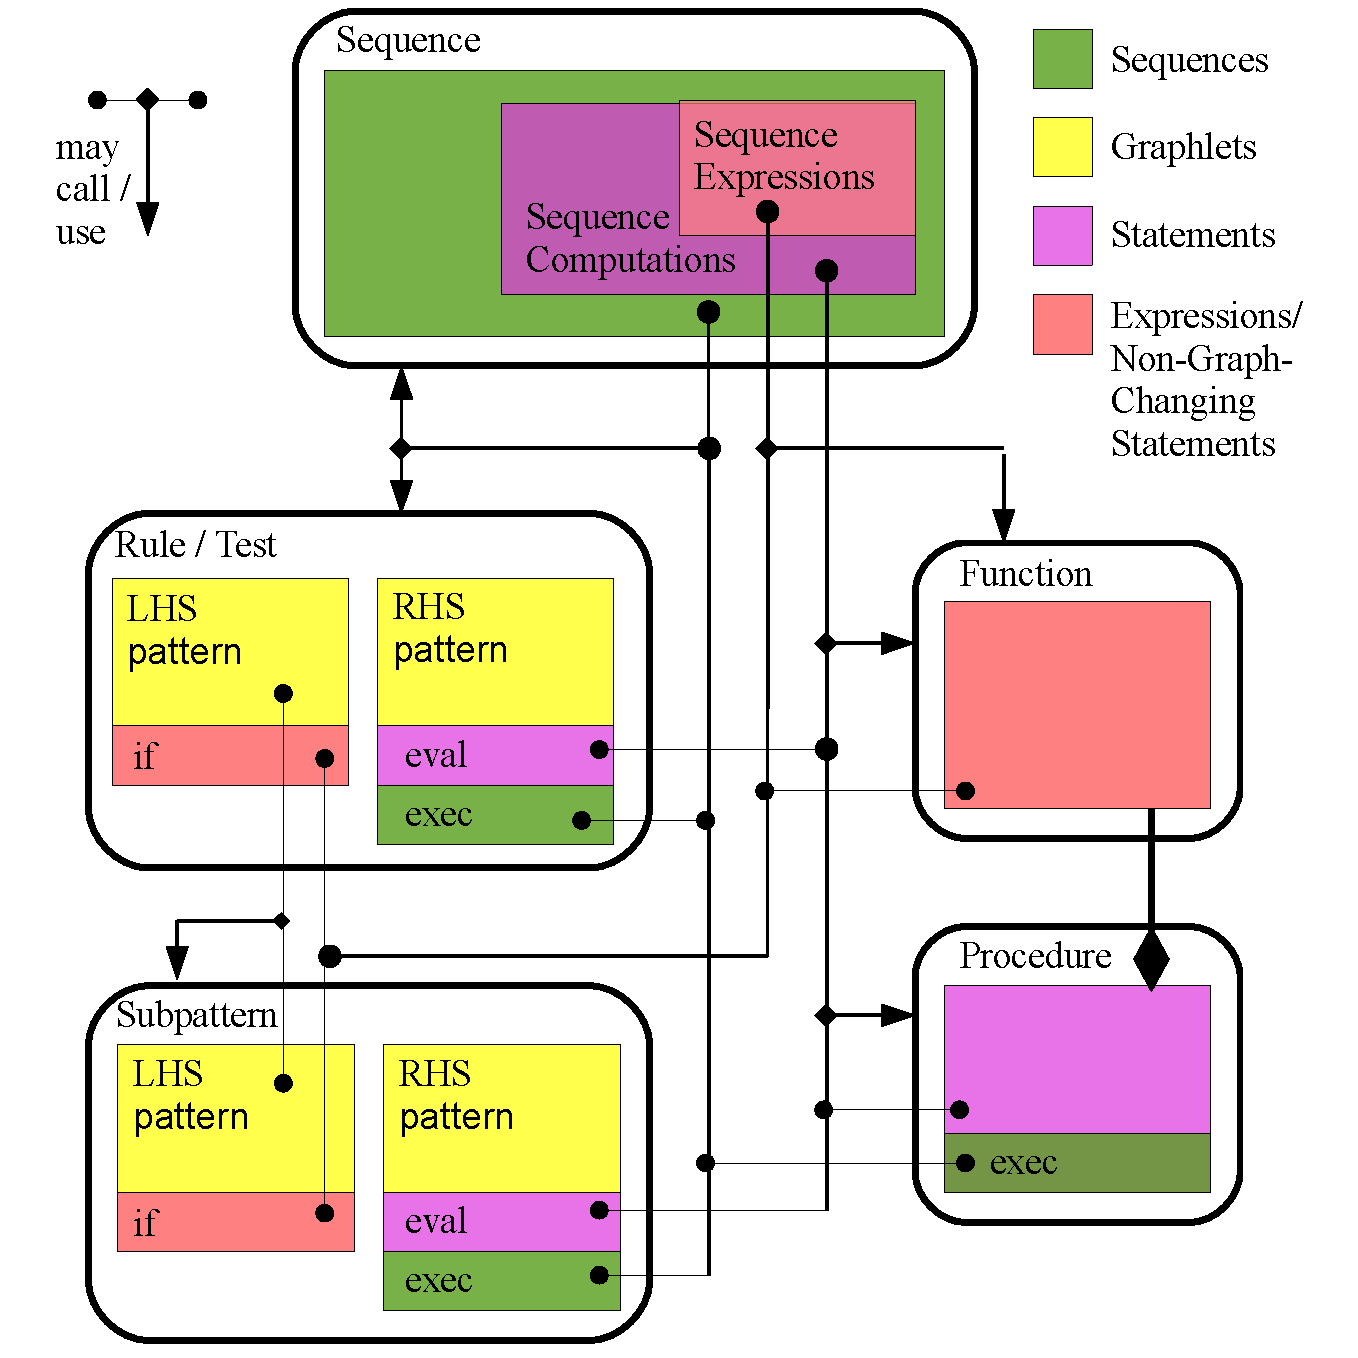
\includegraphics[width=1.0\textwidth]{fig/ComputationContainmentAndCallability}
  \caption{Computation Types and Possible Calls/Uses}
  \label{figcomptypescallsuses}
\end{figure}

The following tables give an overview over the rule and computation sublanguages of \GrG;
separated into pattern and rewrite part, and into expressions and statements.

 %\makeatletter
\begin{table}[htbp]
\begin{minipage}{\linewidth} \renewcommand{\footnoterule}{} 
\begin{tabularx}{\linewidth}{|lX|}
\hline
\texttt{.}	& Declaration of an anonymous node of type \texttt{Node}, to be matched. \\
\texttt{-->}	& Declaration of an anonymous edge of type \texttt{Edge}, to be matched. \\
\texttt{<-->}	& Declaration of an anonymous edge of type \texttt{Edge} that can get matched in either direction. \\
\texttt{--}	& Declaration of an anonymous undirected edge of type \texttt{UEdge}, to be matched. \\
\texttt{n:N} & Declaration of a node \texttt{n} of type \texttt{N}, to be matched.\\
\texttt{-e:E->} & Declaration of an edge \texttt{e} of type \texttt{E}, to be matched.\\
\texttt{n} & Reference to node \texttt{n} within a graphlet.\\
\texttt{-e->} & Reference to edge \texttt{e} within a graphlet.\\
\texttt{def var v:B}	& Defines a def-variable \texttt{v} of basic type \texttt{B}, to be yielded to.\\
\texttt{def ref c:C}	& Defines a def-variable \texttt{c} of container type \texttt{C}, to be yielded to.\\
\hline
\texttt{x:typeof(y)} & The element \texttt{x} to be matched must be of the same or a subtype as \texttt{y}.\\
\texttt{x:T{\textbackslash}S} & The element \texttt{x} must be of type \texttt{T} but not of subtype \texttt{S}.\\
\texttt{x:T<y>} & The element \texttt{y} casted to \texttt{T}, accessible as \texttt{x}.\\
\hline
\texttt{hom(x,y)} & The pattern elements \texttt{x} and \texttt{y} are allowed to match the same graph element.\\
\texttt{independent(x)} & The pattern element \texttt{x} may be matched homomorphically to all other pattern elements.\\
\texttt{exact(x,y)} & All edges incident to \texttt{x} and \texttt{y} in the host graph must have been specified in the pattern.\\
\texttt{induced(x,y)} & Induced edges in between \texttt{x} and \texttt{y} in the host graph must have been specified in the pattern.\\
\hline
\texttt{if\{exp;\}} & An attribute condition constraining the pattern.\\
\texttt{yield\{stmt\}} & A computation for yielding to def variables.\\
\hline
\texttt{nested\{pattern\}} & A nested pattern, with \texttt{nested} being one of the pattern construction modi listed in \ref{keywordregexpsyntax}.\\
\hline
\texttt{p:P()} & A usage/call \texttt{p} of a (user-defined) subpattern of type \texttt{P}.\\
\hline
\end{tabularx}
\end{minipage}\\
\\ 
{\small Let \texttt{exp} be an expression, \texttt{stmt} be a statement, and \texttt{pattern} be a LHS pattern.}
\caption{Pattern (LHS) elements at a glance}
\label{patternstab}
\end{table}
%\makeatother

 %\makeatletter
\begin{table}[htbp]
\begin{minipage}{\linewidth} \renewcommand{\footnoterule}{} 
\begin{tabularx}{\linewidth}{|lX|}
\hline
\texttt{modify\{pattern\}}	& An RHS pattern nested in an arbitrary LHS pattern, specifying the changes. \\
\texttt{replace\{pattern\}}	& An RHS pattern nested in an arbitrary LHS pattern, specifying the target pattern. \\
\hline
\texttt{.}	& Declaration of an anonymous node of type \texttt{Node}, to be created. \\
\texttt{-->}	& Declaration of an anonymous edge of type \texttt{Edge}, to be created. \\
\texttt{n:N} & Declaration of a node \texttt{n} of type \texttt{N}, to be created.\\
\texttt{-e:E->} & Declaration of an edge \texttt{e} of type \texttt{E}, to be created.\\
\texttt{n} & Reference to node \texttt{n} within a graphlet, ensures it is kept in \texttt{replace} mode.\\
\texttt{-e->} & Reference to edge \texttt{e} within a graphlet, ensures it is kept in \texttt{replace} mode.\\
\texttt{def var v:B}	& Defines a def-variable \texttt{v} of basic type \texttt{B}, to be yielded to.\\
\texttt{def ref c:C}	& Defines a def-variable \texttt{c} of container type \texttt{C}, to be yielded to.\\
\texttt{delete(x)} & Deletes element \texttt{x} in \texttt{modify} mode.\\
\hline
\texttt{x:typeof(y)} & The element \texttt{x} is created with the same type as \texttt{y}.\\
\texttt{x:T<y>} & The element \texttt{y} is casted to type \texttt{T}, accessible as \texttt{x} afterwards.\\
\texttt{x:copy<y>} & The element \texttt{x} is created as exact copy of \texttt{y}.\\
\texttt{x:typeof(y)<y,z>} & The nodes \texttt{y} and \texttt{z} are merged and casted to the original type of \texttt{y}, accessible as \texttt{x} afterwards.\\
\texttt{x !-e->! y} & The edge \texttt{e} is redirected to source node \texttt{x} and target node \texttt{y}.\\
\hline
\texttt{eval\{stmt\}} & A computation assigning to attributes or def variables.\\
\hline
\texttt{exec(s ;> yield o=i)} & Executes the sequence \texttt{s}, and then yields the value of an inner variable \texttt{i} to an outer variable \texttt{o}. Yielding from an \texttt{exec} is only possible in the top-level \texttt{exec} of a rule, in nested patterns and subpatterns the \texttt{exec} is executed deferred.\\
\hline
\texttt{delete(p)} & Deletes the subpattern used as \texttt{p}.\\
\texttt{:P()} & Creates a simple subpattern of type \texttt{P}.\\
\texttt{:p()} & Uses or calls the rewrite part of a (user-defined) subpattern used as \texttt{p} in the containing LHS pattern.\\
\hline
\end{tabularx}
\end{minipage}\\
\\ 
{\small Let \texttt{stmt} be a statement.}
\caption{Rewrite elements (RHS pattern) at a glance}
\label{rewritestab}
\end{table}
%\makeatother

%\makeatletter
\begin{table}[htbp]
\begin{minipage}{\linewidth} \renewcommand{\footnoterule}{} 
\begin{tabularx}{\linewidth}{|lX|}
\hline
\texttt{v}	& Reads the variable \texttt{v}. \\
\texttt{::v}	& Reads the global variable \texttt{v}. \\
\texttt{v.a} & Reads the attribute \texttt{a} of \texttt{v}.\\
\texttt{v[i]} & Reads the value at position \texttt{i} of container \texttt{v}.\\
\texttt{x.a[i]} & Reads the value at position \texttt{i} of container attribute \texttt{a} of \texttt{x}.\\
\texttt{x.visited[i]} & Reads the visited flag \texttt{i} of graph element \texttt{x}.\\
\hline
\texttt{typeof(v)}	& Returns the type of graph element \texttt{v}. \\
\texttt{(T)v}	& Casts \texttt{v} to type \texttt{T}. \\
\texttt{nameof(v)}	& Returns the name of graph element \texttt{v}. \\
\texttt{random()}	& Returns a random value in between 0.0 and 1.0. \\
\hline
\texttt{cond ? exp1 :~exp2}	& Returns \texttt{exp1} if \texttt{cond}, otherwise \texttt{exp2}. \\
\texttt{e op f}	& For \texttt{op} being one of the binary operators listed in \ref{tabopprios}. \\
\texttt{op f}	& For \texttt{op} being one of the unary operators listed in \ref{tabopprios}. \\
\hline
\texttt{f(...)}	& Calls one of the functions listed in \ref{funcstab}. Or calls a user defined function \texttt{f}. \\
\texttt{v.fm(...)}	& Calls one of the function methods listed in \ref{funcmethstab}. Or calls a user defined function method \texttt{fm}.\\
\hline
\end{tabularx}
\end{minipage}\\
\\ 
{\small Let \texttt{cond}, \texttt{exp1}, and \texttt{exp2} be expressions.}
\caption{Expressions at a glance}
\label{expressionstab}
\end{table}
%\makeatother

 %\makeatletter
\begin{table}[htbp]
\begin{minipage}{\linewidth} \renewcommand{\footnoterule}{} 
\begin{tabularx}{\linewidth}{|lX|}
\hline
\texttt{def n:N}	& Defines a variable \texttt{n} of node type \texttt{N}.\\
\texttt{def -e:E->}	& Defines a variable \texttt{e} of edge type \texttt{E}.\\
\texttt{def var v:B}	& Defines a variable \texttt{v} of basic type \texttt{B}.\\
\texttt{def ref c:C}	& Defines a variable \texttt{c} of container type \texttt{C}.\\
\hline
\texttt{v = exp} & Assigns the value of \texttt{exp} to the variable \texttt{v}.\\
\texttt{::v = exp} & Assigns the value of \texttt{exp} to the global variable \texttt{v}.\\
\texttt{v.a = exp} & Assigns the value of \texttt{exp} to the attribute \texttt{a} of \texttt{v}.\\
\texttt{v[i] = exp} & Assigns the value of \texttt{exp} to the position \texttt{i} of container \texttt{v}.\\
\texttt{x.a[i] = exp} & Assigns the value of \texttt{exp} to the position \texttt{i} of container attribute \texttt{a} of \texttt{x}.\\
\texttt{x.visited[i] = exp} & Assigns the value of \texttt{exp} to the visited flag \texttt{i} of graph element \texttt{x}.\\
\hline
\texttt{if(cond) \{S1\} else \{S2\}} & Executes \texttt{S1} iff \texttt{cond} evaluates to \texttt{true}, or \texttt{S2} otherwise.\\
\texttt{while(cond) \{S1\} } & Executes \texttt{S1} as long as \texttt{cond} evaluates to s\texttt{true}.\\
\texttt{do \{S1\} while(cond) } & Executes \texttt{S1} until \texttt{cond} evaluates to \texttt{false}.\\
\texttt{for(v:T in c) \{S1\} } & Executes \texttt{S1} for each value \texttt{v} contained in container \texttt{c}.\\
\texttt{for(i:T->v:S in c) \{S1\} } & Executes \texttt{S1} for each key/position to value pair \texttt{(i,v)} contained in container \texttt{c}.\\
\hline
\texttt{break} & Aborts execution of the containing loop.\\
\texttt{continue} & Continues execution of the containing loop at its condition.\\
\texttt{return} & Returns from a containing function or procedure.\\
\texttt{return(v)} & Returns from a containing function or procedure with result value \texttt{v}.\\
\hline
\texttt{exec(s ;> yield o=i)} & Executes the sequence \texttt{s}, and then yields the value of an inner variable \texttt{i} to an outer variable \texttt{o}.\\
\hline
\texttt{(...)=p(...)}	& Calls one of the procedures listed in \ref{procstab}. Or calls a user defined procedure \texttt{p}.\\
\texttt{(...)=v.pm(...)}	& Calls one of the procedure methods listed in \ref{procmethstab}. Or calls a user defined procedure method \texttt{pm}.\\
\hline
\texttt{exec(s)} & Executes the sequence \texttt{s}.\\
\hline
\end{tabularx}
\end{minipage}\\
\\ 
{\small Let \texttt{exp} and \texttt{cond} be expressions, and \texttt{S1} and \texttt{S2} be statements}
\caption{Statements at a glance}
\label{statementstab}
\end{table}
%\makeatother





\chapter{Container Types and Computations}
\label{cha:container}\indexmain{storage}


%%%%%%%%%%%%%%%%%%%%%%%%%%%%%%%%%%%%%%%%%%%%%%%%%%%%%%%%%%%%%%%%%%%%%%%%%%%%%%%%%%%%%%%%%%%%%%%%
\section{Built-In Types and Concept of Containers}
\label{sec:builtingenerictypes}
Besides the types already introduced, \GrG\ supports the built-in \indexed{generic types}\indexmainsee{built-in generic types}{generic types} in Table~\ref{builtingenerictypes}.
The exact type format is \indexed{backend} specific.
The \indexed{LGSPBackend} maps the generic types to generic C\#-Dictionaries (i.e. hashmaps) or generic C\#-Lists (misnamed dynamic arrays) or a \GrG\ supplied generic C\#-Deque of their corresponding primitive types, with \texttt{de.unika.ipd.grGen.libGr.SetValueType} as target type for sets, only used with the value \texttt{null}.

\begin{table}[htbp]
\begin{tabularx}{\linewidth}{|l|X|}
	\hline
	\texttt{\indexed{set}<T>} & A (mathematical) set of type \texttt{T}, where \texttt{T} may be an enumeration type or one of the primitive types from \ref{sec:builtintypes}; it may even be a node or edge or graph type, then we speak of storages. \\
	\texttt{\indexed{map}<S,T>} & A (mathematical) map from type \texttt{S} to type \texttt{T}, where \texttt{S} and \texttt{T} may be enumeration types or one of the primitive types from \ref{sec:builtintypes}; it may even be a node or edge or graph type, then we speak of storages. \\
	\texttt{\indexed{array}<T>} & An array of type \texttt{T}, where \texttt{T} may be an enumeration type or one of the primitive types from \ref{sec:builtintypes}; it may even be a node or edge or graph type, then we speak of storages. Shares some similarities with \texttt{map<int,T>}. \\
	\texttt{\indexed{deque}<T>} & A deque of type \texttt{T}, where \texttt{T} may be an enumeration type or one of the primitive types from \ref{sec:builtintypes}; it may even be a node or edge or graph type, then we speak of storages. Shares some similarities with \texttt{array<T>}. \\
	\hline
\end{tabularx}
\caption{\GrG\ built-in generic types}
\label{builtingenerictypes}
\end{table}

The four container types supported by GrGen share a lot of conceptual similarities and can be accessed in a similar way.
They support multiple methods to update them:
\texttt{add} to add an element to the container,
\texttt{rem} to remove an element from the container,
and \texttt{clear} to remove all elements from the container.
Furthermore, they support multiple methods to query them:
\texttt{size} to return the count of elements in the container,
\texttt{empty} to return whether the container is empty or not,
and \texttt{peek} to return an element from the container.

In addition to those common methods there is special syntax support available.
Left associative binary expressions allow to compute a new container from two input containers, or to compare two containers.
Indexed access returns an element at an index position, and indexed assignment overwrites an element at a specified position with another one.
Container typed variables as such may be assigned a container, employing value semantics.
Compound assignments combine a binary expression with an assignment.
The \texttt{in} operator allows to query for containment.
Constructor literals may be used to create and initialize containers.
And finally iteration over the elements in the container is supported with a \texttt{for} loop.
These operations are available in the rule language, as an extension of the expressions from \ref{cha:typeexpr} and the computation statements from \ref{cha:computations}; 
most of them are available in the sequence computations language, too
(\ref{sec:storages} will tell about the differences compared to the rule language).
In the \texttt{if} attribute evaluation clause only side-effect free container queries are allowed.
In the following the container operations will be explained in detail for one type after another.


%%%%%%%%%%%%%%%%%%%%%%%%%%%%%%%%%%%%%%%%%%%%%%%%%%%%%%%%%%%%%%%%%%%%%%%%%%%%%%%%%%%%%%%%%%%%%%%%
\section{Set Operations}\label{sec:setexpr}

Set expressions consist of the known mathematical set operations, plus some operations in method call notation.

\begin{rail}
  SetExpr: PrimaryExpr (MethodSelector)? | Expr 'in' SetExpr | SetExpr SetOperator SetExpr ;
  MethodCall: SetEntity MethodSelector ;
  Assignment: SetEntity '=' SetExpr ;
  CompoundAssignment: SetEntity SetOperator '=' Expr ChangeAssignment? ;
  SetConstructor: ('set' '<' Type '>')? \\ lbrace ( Expression*',' ) rbrace ;
\end{rail}\ixnterm{MethodCall}\ixnterm{SetExpr}\ixkeyw{in}\ixnterm{SetOperator}\ixnterm{CompoundAssignment}\ixnterm{SetConstructor}

\noindent The query method calls on sets are:

\begin{description}
\item[\texttt{.size()}] returns the number of elements in the set, as \texttt{int}
\item[\texttt{.empty()}] returns whether the set is empty, as \texttt{boolean}
\item[\texttt{.peek(num)}] returns the element which comes at position \texttt{num:int} in the sequence of enumeration, as \texttt{T} for \verb#set<T>#; the higher the number, the longer retrieval takes
\end{description}

\noindent The update method calls on sets are:

\begin{description}
\item[Set addition:] \texttt{s.add(v)} adds the value \texttt{v} to the set \texttt{s}.
\item[Set removal:] \texttt{s.rem(v)} removes the value \texttt{v} from the set \texttt{s}.
\item[Set clearing:] \texttt{s.clear()} removes all values from the set \texttt{s}.
\end{description}

\noindent The binary set operators are:

\begin{table}[htbp]
  \centering
  %\begin{tabularx}{0.45\linewidth}{|ll|} \hline
  \begin{tabular}[c]{|ll|} \hline
    \begin{tabular}[c]{l} \verb#|# \end{tabular} & \begin{tabular}[c]{l}Set union (contained in resulting set as soon as contained in one of the sets)\end{tabular}\\ \hline
    \begin{tabular}[c]{l} \verb#&# \end{tabular} & \begin{tabular}[c]{l}Set intersection (contained in resulting set only if contained in both of the sets)\end{tabular} \\ \hline
    \begin{tabular}[c]{l} \verb#\# \end{tabular} & \begin{tabular}[c]{l}Set difference (contained in resulting set iff contained in left but not right set)\end{tabular} \\ \hline
  \end{tabular}
  \caption{Binary set operators, in ascending order of precedence}\indexmain{order of precedence}
  \label{tabsetbinops}
\end{table}

The binary set operators require the left and right operands to be of identical type \verb#set<T>#.
The operator \texttt{x in s} denotes set membership $x \in s$, returning whether the set contains the given element, as \texttt{boolean}.
Furthermore, the container may be iterated over with a \texttt{for} loop, as introduced in  \ref{sub:controlflow}.
The set only allows for non-indexed iteration.

The relational expressions (already introduced in \ref{sec:relational}) used to compare enitites of different kinds, mapping them to the type boolean, are extended to sets according to table~\ref{compset}:
Some set \texttt{A} is a subset of \texttt{B} iff all elements in \texttt{A} are contained in \texttt{B}, too.

\begin{table}[htbp]
  \centering
  \begin{tabularx}{\linewidth}{|l|X|} \hline
    \texttt{A == B} & True, iff $A$ and $B$ are identical. \\
    \texttt{A != B} & True, iff $A$ and $B$ are not identical. \\
    \texttt{A <\ \ B} & True, iff $A$ is a subset of $B$, but $A$ and $B$ are not identical. \\
    \texttt{A >\ \ B} & True, iff $A$ is a superset of $B$, but $A$ and $B$ are not identical. \\
    \texttt{A <= B} & True, iff $A$ is a subset of $B$ or $A$ and $B$ are identical. \\
    \texttt{A >= B} & True, iff $A$ is a superset of $B$ or $A$ and $B$ are identical. \\ \hline
  \end{tabularx}
  \caption{Binary set operators for comparison}
  \label{compset}
\end{table}

The assignments implement the computation constructs introduced in \ref{cha:computations}.
The pure assignment overwrites the target set with the source set, commonly with value semantics, creating a copy of the source set. Only if a local variable (i.e. not an attribute) is assigned to a local variable, is reference semantics used (i.e. both variables point afterwards to the same set).
Compound assignments are assignments which use the first source as target, too,
only adapting the target value instead of computing a new value and overwriting the target with it.
For scalars this is not supported, but for container valued entities it is offered due to the potential for massive computational cost savings.
The compound assignment statements on sets are a set union \verb#|=#, intersection \verb#&=# and difference \verb#\=# assignment.

\begin{rail}
  ChangeAssignment: ('=' '>' | '|' '>' | ampersand '>') (NodeOrEdge '.' BoolAttribute | BoolVariable | VisitedFlag) ;
\end{rail}\ixnterm{ChangeAssignment}

The compound assignments on sets and maps may be enhanced with a change assignment declaration.
The change value is \texttt{true} in case the target collection changes and \texttt{false} in case the target collection is not altered.
The assign-to operator \verb#=># assigns the change value to the specified target, the or-to operator \verb#|># assigns the boolean disjunction of the change value target with the change value to the change value target, the and-to operator \verb#&># assigns the boolean conjunction of the change value target with the change value to the change value target.
This addition allows for efficient data flow computations not needing to check for a change by set comparison, see \ref{subsub:flow}.

The \emph{SetConstructor} extends the \emph{Literal} from \ref{literaldef} (as a refinement of the \emph{ContainerConstructor} there).
It is constant if only primitive type literals, enum literals, or constant expressions are used; this is required for container initializations in the model.
It is non-constant if it contains nodes/edges/or member accesses, which may be the case if used in the rules.
If the type of the container is given before the constructor, the elements given in the type constructor are casted to the specified member types if needed and possible.
Without the type prefix all elements given in the constructor must be of the same type.

\begin{note}
To add a value to a set you may use set union with a single valued set constructor,
to remove a value from a set you may use set difference with a single valued set constructor.
\begin{grgen}
s | { "foo" }
s \ { n.a }
\end{grgen}
Used in this way they get internally optimized to the imperative set addition \texttt{s.add(x)} and removal \texttt{s.rem(x)} methods available in the \texttt{eval} block and the XGRS.
\end{note}


%%%%%%%%%%%%%%%%%%%%%%%%%%%%%%%%%%%%%%%%%%%%%%%%%%%%%%%%%%%%%%%%%%%%%%%%%%%%%%%%%%%%%%%%%%%%%%%%
\section{Map Operations} \label{sec:mapexpr}

Map expressions consist of the known mathematical set operations extended to maps, and map value lookup, plus some operations in method call notation.

\begin{rail}
  MapExpr: PrimaryExpr (MethodSelector)? | Expr 'in' MapExpr | MapExpr '[' Expr ']' | MapExpr MapOperator MapExpr ;
  MethodCall: MapEntity MethodSelector ;
  Assignment: MapEntity '=' MapExpr ;
  IndexedAssignment: MapEntity '[' IndexExpr ']' '=' Expr ;
  CompoundAssignment: MapEntity MapOperator '=' Expr ChangeAssignment? ;
  MapConstructor: ('map' '<' Type ',' Type '>')? \\ lbrace ( (Expression '->' Expression)*',' ) rbrace ;
\end{rail}\ixnterm{MethodCall}\ixnterm{MapExpr}\ixkeyw{in}\ixnterm{MapOperator}\ixnterm{IndexedAssignemt}\ixnterm{CompoundAssignment}\ixnterm{MapConstructor}

\noindent The query method calls on maps are:

\begin{description}
\item[\texttt{.size()}] returns the number of elements in the map, as \texttt{int}
\item[\texttt{.empty()}] returns whether the map is empty, as \texttt{boolean}
\item[\texttt{.peek(num)}] returns the key of the element which comes at position \texttt{num:int} in the sequence of enumeration, as \texttt{S} for \verb#map<S,T>#; the higher the number, the longer retrieval takes
\item[\texttt{.domain()}] returns the set of elements in the domain of the map, as \verb#set<S># for \verb#map<S,T>#
\item[\texttt{.range()}] returns the set of elements in the range of the map, as \verb#set<T># for \verb#map<S,T>#
\end{description}

\noindent The update method calls on maps are:

\begin{description}
\item[Map addition:] \texttt{m.add(k,v)} adds the pair (\texttt{k},\texttt{v}) to the map \texttt{m}, overwrites the old value if a pair (\texttt{k},unknown) was already existing.
\item[Map removal:] \texttt{m.rem(k)} removes the pair (\texttt{k},unknown) from the map \texttt{m}.
\item[Map clearing:] \texttt{m.clear()} removes all values from the map \texttt{m}.
\end{description}

\noindent The binary map operators are:

\begin{table}[htbp]
  \centering
  %\begin{tabularx}{0.45\linewidth}{|ll|} \hline
  \begin{tabular}[c]{|ll|} \hline
    \begin{tabular}[c]{l} \verb#|# \end{tabular} & \begin{tabular}[c]{l}Map union: returns new map with elements which are in at least one of the maps,\\ with the value of map2 taking precedence\end{tabular}\\ \hline
    \begin{tabular}[c]{l} \verb#&# \end{tabular} & \begin{tabular}[c]{l}Map intersection: returns new map with elements which are in both maps,\\ with the value of map1 taking precedence\end{tabular} \\ \hline
    \begin{tabular}[c]{l} \verb#\# \end{tabular} & \begin{tabular}[c]{l}Map difference: returns new map with elements from map1\\ without the elements with a key contained in map2\end{tabular}\\ \hline
  \end{tabular}
  \caption{Binary map operators, in ascending order of precedence}\indexmain{order of precedence}
  \label{tabmapbinops}
\end{table}

The binary map operators require the left and right operands to be of identical type \verb#map<S,T>#,
with one exception for map difference, this operator accepts for a left operand of type \verb#map<S,T># a right operand of type \verb#set<S>#, too.
The operator \texttt{x in m} denotes map domain membership $x \in dom(m)$, returning whether the domain of the map contains the given element, as \texttt{boolean}.
The operator \texttt{m[x]} denotes map lookup, i.e. it returns the value \texttt{y} which is stored in the map \texttt{m} for the value \texttt{x} (domain value \texttt{x} is mapped by the mapping \texttt{m} to range value \texttt{y}). The value \texttt{x} \emph{must} be in the map, i.e. \texttt{x in m} must hold.
Furthermore, the container may be iterated over with a \texttt{for} loop, as introduced in  \ref{sub:controlflow}.
The map only allows for indexed iteration, with the key getting assigned to the index variable and the corresponding value getting assigned to the value variable.

The relational expressions (already introduced in \ref{sec:relational}) used to compare enitites of different kinds, mapping them to the type boolean, are extended to sets according to table~\ref{compmap}:
A map \texttt{A} is a submap of \texttt{B} iff all key-value pairs of \texttt{A} are contained in \texttt{B}, too. If they have a key in common but map to a different value, they count as not identical.

\begin{table}[htbp]
  \centering
  \begin{tabularx}{\linewidth}{|l|X|} \hline
    \texttt{A == B} & True, iff $A$ and $B$ are identical. \\
    \texttt{A != B} & True, iff $A$ and $B$ are not identical. \\
    \texttt{A <\ \ B} & True, iff $A$ is a submap of $B$, but $A$ and $B$ are not identical. \\
    \texttt{A >\ \ B} & True, iff $A$ is a supermap of $B$, but $A$ and $B$ are not identical. \\
    \texttt{A <= B} & True, iff $A$ is a submap of $B$ or $A$ and $B$ are identical. \\
    \texttt{A >= B} & True, iff $A$ is a supermap of $B$ or $A$ and $B$ are identical. \\ \hline
  \end{tabularx}
  \caption{Binary map operators for comparison}
  \label{compmap}
\end{table}

The assignments implement the computation constructs introduced in \ref{cha:computations}.
The pure assignment overwrites the target map with the source map, commonly with value semantics, creating a copy of the source map. Only if a local variable (i.e. not an attribute) is assigned to a local variable, is reference semantics used  (i.e. both variables point afterwards to the same map).
The indexed assignment \texttt{m[i]=v} overwrites the old value at index \texttt{i} in the map \texttt{m} with the new value \texttt{v}.
Compound assignments are assignments which use the first source as target, too,
only adapting the target value instead of computing a new value and overwriting the target with it.
For scalars this is not supported, but for container valued entities it is offered due to the potential for massive computational cost savings.
The compound assignment statements on maps are a map union \verb#|=#, intersection \verb#&=# and difference \verb#\=# assignment.

The \emph{MapConstructor} extends the \emph{Literal} from \ref{literaldef} (as a refinement of the \emph{ContainerConstructor} there).
It is constant if only primitive type literals, enum literals, or constant expressions are used; this is required for container initializations in the model.
It is non-constant if it contains nodes/edges/or member accesses, which may be the case if used in the rules.
If the type of the container is given before the constructor, the elements given in the type constructor are casted to the specified member types if needed and possible.
Without the type prefix all elements given in the constructor must be of the same type.

\begin{note}
To add a (key,value)-pair to a map you may use map union with a single valued map constructor,
to remove a value from a map you may use map difference with a single valued set or map constructor.
\begin{grgen}
m | { "foo" -> 42 }
m \ { n.a -> n.b } or m \ { n.a }
\end{grgen}
Used in this way they get internally optimized to the imperative map addition \texttt{s.add(key,value)} and removal \texttt{s.rem(key)} methods available in the \texttt{eval} block and the XGRS.
\end{note}


%%%%%%%%%%%%%%%%%%%%%%%%%%%%%%%%%%%%%%%%%%%%%%%%%%%%%%%%%%%%%%%%%%%%%%%%%%%%%%%%%%%%%%%%%%%%%%%%
\section{Array Operations} \label{sec:arrayexpr}

Array expressions consist of array membership checking, array value lookup, and array concatenation, plus some operations in method call notation.

\begin{rail}
  ArrayExpr: PrimaryExpr (MethodSelector)? | Expr 'in' ArrayExpr | ArrayExpr '[' Expr ']' | ArrayExpr ArrayOperator ArrayExpr;
  MethodCall: ArrayEntity MethodSelector ;
  Assignment: ArrayEntity '=' ArrayExpr ;
  IndexedAssignment: ArrayEntity '[' IndexExpr ']' '=' Expr ;
  CompoundAssignment: ArrayEntity ArrayOperator '=' Expr ChangeAssignment? ;
  ArrayConstructor: ('array' '<' Type '>')? \\ '[' ( Expression*',' ) ']' ;
\end{rail}\ixnterm{MethodCall}\ixnterm{ArrayExpr}\ixkeyw{in}\ixnterm{ArrayOperator}\ixnterm{IndexedAssignemt}\ixnterm{CompoundAssignment}\ixnterm{ArrayConstructor}

\noindent The query method calls on arrays are:

\begin{description}
\item[\texttt{.size()}] returns the number of elements in the array, as \texttt{int}
\item[\texttt{.empty()}] returns whether the array is empty, as \texttt{boolean}
\item[\texttt{.peek(num)}] returns the value stored in the array at position \texttt{num:int} in the sequence of enumeration, is equivalent to (and implemented by) \texttt{a[num])}; retrieval occurs in constant time.
\item[\texttt{.peek()}] returns the last value stored in the array; retrieval occurs in constant time.
\item[\texttt{.indexOf(valueToSearchFor)}] returns first position \texttt{valueToSearchFor:T} appears at, as \texttt{int}, or -1 if not found
\item[\texttt{.lastIndexOf(valueToSearchFor)}] returns last position \texttt{valueToSearchFor:T} appears at, as \texttt{int}, or -1 if not found
\item[\texttt{.subarray(startIndex, length)}] returns subarray of given \texttt{length:int} from \texttt{startIndex:int} on
\end{description}

\noindent The update method calls on arrays are:

\begin{description}
\item[Array addition:] \texttt{a.add(v)} adds the value \texttt{v} to the end of array \texttt{a}.
\item[Array addition:] \texttt{a.add(v,i)} inserts the value \texttt{v} at index \texttt{i} to array \texttt{a}.
\item[Array removal:] \texttt{a.rem()} removes the value at then end of the array \texttt{a}.
\item[Array removal:] \texttt{a.rem(i)} removes the value at index \texttt{i} from the array \texttt{a}.
\item[Array clearing:] \texttt{a.clear()} removes all values from the array \texttt{a}.
\end{description}

\noindent The binary array operators are:

\begin{table}[htbp]
  \centering
  %\begin{tabularx}{0.45\linewidth}{|ll|} \hline
  \begin{tabular}[c]{|ll|} \hline
    \begin{tabular}[c]{l} \verb#+# \end{tabular} & \begin{tabular}[c]{l}Array concatenation: returns new array with the right appended to the left array\\the left and right operands must be of identical type \verb#array<T>#
    \end{tabular}\\ \hline
  \end{tabular}
  \caption{Binary array operators, in ascending order of precedence}\indexmain{order of precedence}
  \label{tabarraybinops}
\end{table}

The operator \texttt{x in a} denotes array value membership, returning whether the array contains the given element, as \texttt{boolean}.
The operator \texttt{a[x]} denotes array lookup, i.e. it returns the value \texttt{y} which is stored in the array \texttt{a} at the index \texttt{x}.
The index \texttt{x} \emph{must} be a valid array index.
Furthermore, the container may be iterated over with a \texttt{for} loop, as introduced in  \ref{sub:controlflow}.
The array allows for non-indexed as well as indexed iteration; if non-indexed iteration is used the array values are iterated over, if indexed iteration is used the index is assigned to the index variable and the corrsponding value is assigned to the value variable. 

The relational expressions (already introduced in \ref{sec:relational}) used to compare enitites of different kinds, mapping them to the type boolean, are extended to sets according to table~\ref{comparray}:
An array \texttt{A} is a subarray of \texttt{B} iff it is smaller or equal in size and the values at each common index are identical (lexicographic order as for strings).

\begin{table}[htbp]
  \centering
  \begin{tabularx}{\linewidth}{|l|X|} \hline
    \texttt{A == B} & True, iff $A$ and $B$ are identical. \\
    \texttt{A != B} & True, iff $A$ and $B$ are not identical. \\
    \texttt{A <\ \ B} & True, iff $A$ is a subarray of $B$, but $A$ and $B$ are not identical. \\
    \texttt{A >\ \ B} & True, iff $A$ is a superarray of $B$, but $A$ and $B$ are not identical. \\
    \texttt{A <= B} & True, iff $A$ is a subarray of $B$ or $A$ and $B$ are identical. \\
    \texttt{A >= B} & True, iff $A$ is a superarray of $B$ or $A$ and $B$ are identical. \\ \hline
  \end{tabularx}
  \caption{Binary array operators for comparison}
  \label{comparray}
\end{table}

The assignments implement the computation constructs introduced in \ref{cha:computations}.
The pure assignment overwrites the target array with the source array, commonly with value semantics, creating a copy of the source array. Only if a local variable (i.e. not an attribute) is assigned to a local variable, is reference semantics used  (i.e. both variables point afterwards to the same array).
The indexed assignment \texttt{a[i]=v} overwrites the old value at index \texttt{i} in the array \texttt{a} with the new value \texttt{v}.
Compound assignments are assignments which use the first source as target, too,
only adapting the target value instead of computing a new value and overwriting the target with it.
For scalars this is not supported, but for container valued entities it is offered due to the potential for massive computational cost savings.
The compound assignment statement on arrays is the concatenation assignment \verb#+=#.

The \emph{ArrayConstructor} extends the \emph{Literal} from \ref{literaldef} (as a refinement of the \emph{ContainerConstructor} there).
It is constant if only primitive type literals, enum literals, or constant expressions are used; this is required for container initializations in the model.
It is non-constant if it contains nodes/edges/or member accesses, which may be the case if used in the rules.
If the type of the container is given before the constructor, the elements given in the type constructor are casted to the specified member types if needed and possible.
Without the type prefix all elements given in the constructor must be of the same type.

%%%%%%%%%%%%%%%%%%%%%%%%%%%%%%%%%%%%%%%%%%%%%%%%%%%%%%%%%%%%%%%%%%%%%%%%%%%%%%%%%%%%%%%%%%%%%%%%
\section{Deque Operations} \label{sec:dequeexpr}

Deque expressions consist of deque membership checking, deque value lookup, and deque concatenation, plus some operations in method call notation.

\begin{rail}
  DequeExpr: PrimaryExpr (MethodSelector)? | Expr 'in' DequeExpr | DequeExpr '[' Expr ']' | DequeExpr DequeOperator DequeExpr;
  MethodCall: DequeEntity MethodSelector ;
  Assignment: DequeEntity '=' DequeExpr ;
  IndexedAssignment: DequeEntity '[' IndexExpr ']' '=' Expr ;
  CompoundAssignment: DequeEntity DequeOperator '=' Expr ChangeAssignment? ;
  DequeConstructor: ('deque' '<' Type '>')? \\ ']' ( Expression*',' ) '[' ;
\end{rail}\ixnterm{MethodCall}\ixnterm{DequeExpr}\ixkeyw{in}\ixnterm{DequeOperator}\ixnterm{IndexedAssignemt}\ixnterm{CompoundAssignment}\ixnterm{DequeConstructor}

\noindent The query method calls on deques are:

\begin{description}
\item[\texttt{.size()}] returns the number of elements in the deque, as \texttt{int}
\item[\texttt{.empty()}] returns whether the deque is empty, as \texttt{boolean}
\item[\texttt{.peek(num)}] returns the value stored in the deque at position \texttt{num:int} in the sequence of enumeration, is equivalent to (and implemented by) \texttt{a[num])}; retrieval occurs in constant time.
\item[\texttt{.peek()}] returns the first value stored in the deque; retrieval occurs in constant time.
\item[\texttt{.indexOf(valueToSearchFor)}] returns first position \texttt{valueToSearchFor:T} appears at, as \texttt{int}, or -1 if not found
\item[\texttt{.lastIndexOf(valueToSearchFor)}] returns last position \texttt{valueToSearchFor:T} appears at, as \texttt{int}, or -1 if not found
\item[\texttt{.subdeque(startIndex, length)}] returns subdeque of given \texttt{length:int} from \texttt{startIndex:int} on
\end{description}

\noindent The update method calls on deques are:

\begin{description}
\item[Deque addition:] \texttt{d.add(v)} adds the value \texttt{v} to the end of deque \texttt{d}.
\item[Deque addition:] \texttt{d.add(v,i)} inserts the value \texttt{v} at index \texttt{i} to deque \texttt{d}.
\item[Deque removal:] \texttt{d.rem()} removes the value at then begin of the deque \texttt{d}.
\item[Deque removal:] \texttt{d.rem(i)} removes the value at index \texttt{i} from the deque \texttt{d}.
\item[Deque clearing:] \texttt{d.clear()} removes all values from the deque \texttt{d}.
\end{description}

\noindent The binary deque operators are:

\begin{table}[htbp]
  \centering
  %\begin{tabularx}{0.45\linewidth}{|ll|} \hline
  \begin{tabular}[c]{|ll|} \hline
    \begin{tabular}[c]{l} \verb#+# \end{tabular} & \begin{tabular}[c]{l}Deque concatenation: returns new deque with the right appended to the left deque\\the left and right operands must be of identical type \verb#deque<T>#
    \end{tabular}\\ \hline
  \end{tabular}
  \caption{Binary deque operators, in ascending order of precedence}\indexmain{order of precedence}
  \label{tabdequebinops}
\end{table}

The operator \texttt{x in d} denotes deque value membership, returning whether the deque contains the given element, as \texttt{boolean}.
The operator \texttt{d[x]} denotes deque lookup, i.e. it returns the value \texttt{y} which is stored in the deque \texttt{d} at the index \texttt{x}.
The index \texttt{x} \emph{must} be a valid deque index.
Furthermore, the container may be iterated over with a \texttt{for} loop, as introduced in  \ref{sub:controlflow}.
The deque allows for non-indexed as well as indexed iteration; if non-indexed iteration is used the deque values are iterated over, if indexed iteration is used the index is assigned to the index variable and the corrsponding value is assigned to the value variable. 

The relational expressions (already introduced in \ref{sec:relational}) used to compare enitites of different kinds, mapping them to the type boolean, are extended to sets according to table~\ref{compdeque}:
A deque \texttt{A} is a subdeque of \texttt{B} iff it is smaller or equal in size and the values at each common index are identical (lexicographic order as for strings).

\begin{table}[htbp]
  \centering
  \begin{tabularx}{\linewidth}{|l|X|} \hline
    \texttt{A == B} & True, iff $A$ and $B$ are identical. \\
    \texttt{A != B} & True, iff $A$ and $B$ are not identical. \\
    \texttt{A <\ \ B} & True, iff $A$ is a subdeque of $B$, but $A$ and $B$ are not identical. \\
    \texttt{A >\ \ B} & True, iff $A$ is a superdeque of $B$, but $A$ and $B$ are not identical. \\
    \texttt{A <= B} & True, iff $A$ is a subdeque of $B$ or $A$ and $B$ are identical. \\
    \texttt{A >= B} & True, iff $A$ is a superdeque of $B$ or $A$ and $B$ are identical. \\ \hline
  \end{tabularx}
  \caption{Binary deque operators for comparison}
  \label{compdeque}
\end{table}

The assignments implement the computation constructs introduced in \ref{cha:computations}.
The pure assignment overwrites the target deque with the source deque, commonly with value semantics, creating a copy of the source deque. Only if a local variable (i.e. not an attribute) is assigned to a local variable, is reference semantics used  (i.e. both variables point afterwards to the same deque).
The indexed assignment \texttt{d[i]=v} overwrites the old value at index \texttt{i} in the deque \texttt{d} with the new value \texttt{v}.
Compound assignments are assignments which use the first source as target, too,
only adapting the target value instead of computing a new value and overwriting the target with it.
For scalars this is not supported, but for container valued entities it is offered due to the potential for massive computational cost savings.
The compound assignment statement on deques is the concatenation assignment \verb#+=#.

The \emph{DequeConstructor} extends the \emph{Literal} from \ref{literaldef} (as a refinement of the \emph{ContainerConstructor} there).
It is constant if only primitive type literals, enum literals, or constant expressions are used; this is required for container initializations in the model.
It is non-constant if it contains nodes/edges/or member accesses, which may be the case if used in the rules.
If the type of the container is given before the constructor, the elements given in the type constructor are casted to the specified member types if needed and possible.
Without the type prefix all elements given in the constructor must be of the same type.

\begin{note}
The double ended queue allows for fast addition and removal both at the frond and at the back, in contrast to arrays that only support this at the end.
It is implemented by a ringbuffer that is grown as needed, a lookup is slightly more expensive than an array lookup.
The primary usage of the deque is as a queue, as needed for breadth first search, accessed FIFO.
This is in contrast to the array that is suited to be employed as a stack, e.g. in a depth first search (unless that is programmed using the call stack), accessed LIFO.
\end{note}


%%%%%%%%%%%%%%%%%%%%%%%%%%%%%%%%%%%%%%%%%%%%%%%%%%%%%%%%%%%%%%%%%%%%%%%%%%%%%%%%%%%%%%%%%%%%%%%%
\section{Storage Access in the Rules} \label{sub:storageaccess}\indexmain{storage access}

Storages can be used in the rule application control language as introduced above \ref{sec:storages}, they can get filled or emptied in the rules as defined here \ref{replstmt}, a discussion about their usage and examples are given here \ref{sub:mergesplit}, here \ref{subsub:copystructure}, and here \ref{subsub:flow}.
In the pattern part you may ask for an element to get bound to an element from a storage or a storage attribute;
this is syntactically specified by giving the storage enclosed in left and right braces.
You may ask for an element to get bound to the value element queried from a storagemap by a key graph element;
this is syntactically specified by giving the storagemap indexed by the key graph element enclosed in left and right braces
(this is not possible for storage map attributes due to internal limitations with the search planning).
If the type of the element retrieved from the storage is not compatible to the type of the pattern element specified,
or if the storage is empty, or if the key element is not contained in the storagemap, matching fails.

The advantage of this storage querying inside the rule over handing in a value from a for loop iterating the storage values outside the rule are: i) a more concise syntax, ii) the ability to access a storage attribute of an element just matched or to access a storage map with an element just matched in the same rule, which would require to break up the rule in two rules in the other case, and iii), a restriction of the iteration to the matching phase, so that at rewriting one can happily manipulate the storage without destroying the iterator/enumerator used in the loop which would be the case when using an outside loop.

The following syntax diagram gives an extensions to the syntax diagrams of the Rule Set Language chapter \ref{chaprulelang}, pattern part:
\begin{rail}
  StorageAccess:
    lbrace StorageVariable rbrace |
    lbrace NodeOrEdge '.' StorageAttribute rbrace |
    lbrace StorageMap '[' Ident ']' rbrace;
\end{rail}\ixnterm{StorageAccess}

\begin{example}
Queries the graph for the neighbouring cities to the cities contained in the storageset.
\begin{grgen}
test neighbour(ref startCities:set<City>) : City
{
    :City{startCities} -:Street-> n:City;
    return(n);
}
\end{grgen}
\end{example}

\begin{example}
Queries for the neighbour of the neighbour of a city matched.
With the first neigbouring relation queried from the storagemap assumed to contain the neighbouring relation of some cities of interest, and the second neighbouring relation queried from the graph.
\begin{grgen}
test neighbourneighbour(ref neighbours:map<City, City>) : City
{
    someCity:City;
    nc:City{neighbours[someCity]} -:Street-> nnc:City;
    return(nnc);
}
\end{grgen}
\end{example}

%These were the storage queries available in the pattern part.


%%%%%%%%%%%%%%%%%%%%%%%%%%%%%%%%%%%%%%%%%%%%%%%%%%%%%%%%%%%%%%%%%%%%%%%%%%%%%%%%%%%%%%%%%%%%%%%%
\section{Hints on container usage}

%das noch als container hints hintendran, erkl�ren wof�r gut/wof�r nicht
%deklarative vs imperative nutzung.
%also storages nutzung, data flow nutzung, constructoren f�r vergleiche gegen viele werte, wenn constant dann ist das effizient (todo: stimmt f�r regeln, aber auch f�r computations?)
%das zusammenspiel byref/byvalue bei aufrufen, innerhalb der regeln/computations erkl�ren, copy weil graph container changes f�rchterliche nebenwirking w�ren. hinweis: neben addbef�llen gibt es deklarative konstruktoren verf�gbar.

%The by-ref container parameters or container attributes can be operated upon by the container state change methods,
%which allow to only partially change the container by adding or removing or overwriting elements resp. pairs of elements (in contrast to normal assignments which replace overwrite the target variable entirely);
%they are especially useful for containers containing nodes or edges.

\begin{example}
The container state change methods \texttt{add} and \texttt{rem} allow to add graph elements to storages or remove graph elements from storages, i.e. sets or maps or arrays or deques holding nodes and edges used for rewrite in the calling sequence (cf. \ref{sec:storages}).
This way you can write transformations consisting of several passes with one pass operating on nodes/edges determined in a previous pass,
without the need to mark the element in the graph by helper edges or visited flags.
	\begin{grgen}
rule foo(ref storage:set<Node>)
{
  n:Node;
  modify {
    eval {
      storage.add(n);
    }
  }
}
	\end{grgen}
\end{example}

\begin{example}
Some examples of container literals:
\begin{grgen}
{ "foo", "bar" } // a constant set<string> constructor
map<string,int>{ (n.strVal+m.strVal)->(m.intVal+n.intVal), intVal->strVal, "fool"->42 } // a non-constant map constructor with type prefix
[ 1,2,3 ] // a constant array<int> constructor
] 1,2,3 [ // a constant deque<int> constructor
\end{grgen}
\end{example}\label{containerconstructorex}



\chapter{Graph Type and Computations}
\label{cha:graph}\indexmain{visited flag}


%%%%%%%%%%%%%%%%%%%%%%%%%%%%%%%%%%%%%%%%%%%%%%%%%%%%%%%%%%%%%%%%%%%%%%%%%%%%%%%%%%%%%%%%%%%%%%%%
\section{Built-In Types}
\label{sec:builtingenerictypes}
Besides the types already introduced, \GrG\ offers supports for a \texttt{\indexed{graph}} type.
If used explicitly, it denotes a subgraph of the host graph, which can be used for storing and comparing subgraphs of the current host graph. (Because of the "there is only a single host graph"-design of GrGen you must explicitely descend to the nested subgraph if you intend to process it, see \ref{sec:graphnesting}).

But more important are the large number of global functions (with call syntax as already introduced in \ref{sec:primexpr}) and global procedures (with call syntax as already introduced in \ref{sec:proccall}) that implicitly operate on the single host graph (and thus on the graph type).
There are update functions available that allow to manipulate the graph available with \texttt{add}, \texttt{rem} and \texttt{retype}.
The host graph may be queried for all \texttt{nodes} or \texttt{edges} of a given type.
An edge may be queried for its \texttt{source} and \texttt{target} elements,
while a node may be queried for its direct neighbourhood with all \texttt{incident} edges, or all \texttt{adjacent} nodes.
Or even for its transitive neighbourhood with all \texttt{reachable} nodes or edges.
In the form of functions returning \texttt{set}s of nodes or edges, or in the form of iterations with \texttt{for} loops, or in the form of boolean predicates to test the neighbourhood if two elements are given.
The \texttt{induced} subgraph of a set of nodes or edges may be computed, or directly \texttt{insert}ed into the host graph.

Furthermore, \texttt{visited} flags may be used for marking already visited elements during graph walks or for partitioning a graph.
These operations are available in the rule language, as function atoms of the expression sublanguage from \ref{cha:typeexpr}, and as procedure atoms of the statement sublanguage from \ref{cha:computations}; 
most of them are available in the sequence computations language, too
(\ref{sec:seqcomp} will tell about the differences compared to the rule language).

The graph manipulation procedures, the transaction handling procedures, and the visited flag management and assignment procedures are not available in the function abstraction; they may only be called from the procedures.

%%%%%%%%%%%%%%%%%%%%%%%%%%%%%%%%%%%%%%%%%%%%%%%%%%%%%%%%%%%%%%%%%%%%%%%%%%%%%%%%%%%%%%%%%%%%%%%%
\section{Graph Functions And Procedures}\indexmain{graph functions}\indexmain{graph procedures}\label{neighbouringelementsfunctions}

%-----------------------------------------------------------------------------------------------
\subsection{Graph Updates / Basic Graph Manipulation}

There are procedures to update the graph by adding or removing or retyping available, on nodes and edges: 

\begin{description}
\item[\texttt{add(.)}] adds a new node of the given node type to the host graph, returns the added node.
\item[\texttt{addCopy(.)}] adds a clone of the original node to the host graph, returns the added node.
\item[\texttt{add(.,.,.)}] adds a new edge of the given edge type to the host graph, in between the source node specified as second argument and the target node specified as third argument, returns the added edge.
\item[\texttt{addCopy(.,.,.)}] adds a clone of the original edge to the host graph, in between the source node specified as second argument and the target node specified as third argument, returns the added edge.
\item[\texttt{rem(.)}] removes the node or edge given from the host graph (no expression, does not return anything).
\item[\texttt{retype(.,.)}] retypes the node or edge given to the node type or edge type given as second argument, returns the retyped entity.
\item[\texttt{clear()}] clears the host graph.
\end{description}

\noindent Besidse those basic graph manipulation functions, some advanced rewriting operations are available as procedures, too:

\begin{description}
\item[\texttt{merge(.,.)}] merges the source node given as second argument into the target node given as first argument.
\item[\texttt{redirectSource(.,.)}] redirects the edge given as first argument to the new source node given as second argument.
\item[\texttt{redirectTarget(.,.)}] redirects the edge given as first argument to the new target node given as second argument.
\item[\texttt{redirectSourceAndTarget(.,.)}] redirects the edge given as first argument to the new source node given as second argument and the new target node given as third argument.
\end{description}

The versions introduced above are only available on named graphs, as they fetch the debug display name from the old element.
If you want to use them on unnamed graphs you must supply an additional argument giving the name of the old element; in case of the \texttt{redirectSourceAndTarget} you must supply two additional arguments, first the string to use for the old source node name, then the string to use for the old target node name.

%-----------------------------------------------------------------------------------------------
\subsection{Graph Query by Types}

There are functions to ask for all nodes or edges of a type available: 
\begin{description}
\item[\texttt{nodes(.)}] returns all nodes in the graph compatible to the given node type, as set.
\item[\texttt{nodes()}] returns all nodes in the graph, as set.
\item[\texttt{edges(.)}] returns all edges in the graph compatible to the given edge type, as set.
\item[\texttt{edges()}] returns all edges in the graph, as set.
\end{description}

The same functions can be used from for loops to iterate over the entities, omitting the filling of a set: 
\begin{description}
\item[\texttt{for(n:NodyType in nodes(NodeType)) \{Statements\}} ] iterates over all nodes in the graph compatible to the given node type.
\item[\texttt{for(n:Node in nodes()) \{Statements\}} ] iterates over all nodes in the graph.
\item[\texttt{for(e:EdgeType in edges(EdgeType)) \{Statements\}} ] iterates over all edges in the graph compatible to the given edge type.
\item[\texttt{for(e:Edge in edges()) \{Statements\}} ] iterates over all edges in the graph.
\end{description}

%-----------------------------------------------------------------------------------------------
\subsection{Graph Query by Neighbourhood}\label{sub:querybyneighbourhood}

Multiple functions are available to query the neighbourhood of nodes and edges.

\subsubsection*{Edge Neighbourhood}

The nodes incident to a given edge may be queried by the following functions: 

\begin{description}
\item[\texttt{source(.)}] returns the source node of the given edge.
\item[\texttt{target(.)}] returns the target node of the given edge.
\item[\texttt{opposite(.,.)}] returns the opposite node of the edge and the node (second argument) given.
\end{description}

\subsubsection*{Node Neighbourhood Common Concepts}

The edges \texttt{incident} or the nodes \texttt{adjacent} to a given node may be queried.

The neighbourhood query functions allow to additionally constrain the direction of the edges to \texttt{incoming} or \texttt{outgoing} edges, otherwise both directions are accepted.

The neighbourhood query functions furthermore allow to constrain the accepted situations by optional arguments. The type the incident edges must have to be accounted for can be specified. Or the type the incident edges must have to be accounted for and the type the adjacent nodes must have to be accounted for (cf. \ref{NeighbourhoodFunctionCallTypes}).

\begin{rail}
NeighbourhoodFunctionCall: 
  FunctionName '(' StartNodeExpr ')' |
  FunctionName '(' StartNodeExpr ',' EdgeType ')' |
  FunctionName '(' StartNodeExpr ',' EdgeType ',' NodeType ')'
  ;
\end{rail}\label{NeighbourhoodFunctionCallTypes}

The neighbourhood query function can be used in four possible ways: 
\begin{description}
	\item[Set functions:] The neighbourhood function returns a set of neighbouring entities of the start node. It builds a set that is likely thrown away thereafter, so esp. for large sets this functions is less efficient than the other versions.
\begin{rail}
Expression:
  FunctionName '(' StartNodeExpr ')' ;
\end{rail}
	\item[Iteration loops:] The neighbourhood function is employed from a for loop that allows to iterate the neighbouring entities of the start node. No set needs to be built here. But if the source node has multiple edges to a target node, it might be iterated multiple times. And an edge may be iterated twice in case of the undirected functions.
\begin{rail}
ForLoop: 
  'for' '(' Name ':' Type 'in' FunctionName '(' StartNodeExpr ')' \\ lbrace Statements rbrace;
\end{rail}
	\item[Counted functions:] The counted neighbourhood function returns the count of neighbouring entities of the start node. This is at least as efficient as calling \texttt{size()} on the resulting set of the plain neighbourhood function, often it is more efficient.
\begin{rail}
Expression:
  CountedFunctionName '(' StartNodeExpr ')' ;
\end{rail}
The \emph{CountedFunctionName} is built from the \emph{FunctionName} by prepending \texttt{count} and switching the first charecter of \emph{FunctionName} to upper case.
	\item[Boolean functions:] The neighbourhood function is employed in a boolean predicate version that allows the check whether a second target entity is in the queried neighbourhood of the start node. The computation has the smallest internal processing overhead of the three options and stops as soon as a positive result is obtained.
\begin{rail}
Expression:
  FunctionNamePredicate '(' StartNodeExpr ',' TargetEntity ')' ;
\end{rail}
The \emph{FunctionNamePredicate} is built from the \emph{FunctionName} by prepending \texttt{is} and switching the first charecter of \emph{FunctionName} to upper case.
\end{description}


\subsubsection*{Direct Node Neighbourhood}

Available are queries for the neighbouring edges:

\begin{description}
\item[\texttt{incident(.)}] returns the set of the edges that are incident to the node given as argument value.
\item[\texttt{incoming(.)}] same as the incident above, but restricted to incoming edges.
\item[\texttt{outgoing(.)}] same as the incident above, but restricted to outgoing edges.
\end{description}

In the two argument version, only edges of the type given as second argument are contained.
The three argument version behaves as the two argument version, but additionally only edges incident to an opposite node of the type given as third argument are contained.

\begin{example}
\begin{grgen}
rule foo {
    src:Node -e:Edge->; 
    if(!isIncoming(src, e));
    
    modify {
        eval {
            if(incident(src, NiftyEdge, NiftyNode).size()>2)
            {
	              for(ne:NiftyEdge in outgoing(src, NiftyEdge))
	              {
	                  ne.attr = 42;
	              }
	          }
        }
    }
}
\end{grgen}
Some fabricated example showing how to use the incoming, outgoing, and incident functions in their \emph{boolean predicate}, \emph{set function}, and \emph{for iteration} versions, with and without constraining the edge and node types.
\end{example}

Available are queries for the neighbouring nodes:

\begin{description}
\item[\texttt{adjacent(.)}] returns the set of the nodes that are adjacent to the node given as argument value.
\item[\texttt{adjacentIncoming(.)}] same as the adjacent above, but restricted to nodes reachable via incoming edges.
\item[\texttt{adjacentOutgoing(.)}] same as the adjacent above, but restricted to nodes reachable via outgoing edges.
\end{description}

In the two argument version, nodes incident to an edge of the type given as second argument are contained.
The three argument version behaves as the two argument version, but additionally only nodes of the node type given as third argument are contained.

\begin{example}
An example showing how to program a rule by hand with the graph query operations for matching and the graph update operations for rewriting. This is what GrGen does under the covers, and as you can see from the volume and style of code very helpful -- use the pattern language, don't fall back to the computations language unless really needed.
\begin{grgen}
rule example
{
	x:N -e:E-> y:N <--> z:M;
	if { e.a == 42; }

	modify {
		delete(y);
		xn:NN<x>;
		xn --> yn:N --> z;
	}
}
// this procedure behaves similarily to the rule above
procedure example
{
	// match LHS pattern
	def var leave:boolean = false;
	for(x:N in nodes(N)) // lookup n of type N in the graph
	{
		x.visited = true; // (see 14.5 Visited Flags below)
		for(e:E in outgoing(x, E)) // from x on find outgoing edge e of type E
		{
			if(!(e.a == 42)) { // with e.a == 42
				continue;
			}
			def y:Node = target(e); // and target node y of type N
			if(!(typeof(y)<=N)) {
				continue;
			}
			if(y.visited) { // that is not the same as x
				continue;
			}
			for(z:Node in adjacent(y, Edge, M)) // from y on find adjacent node z of type M
			{ // N and M are disjoint, can't match each other, otherwise visited would be needed
			
				// rewrite according to RHS pattern
				rem(y);
				(def xn:NN)=retype(x,NN);
				(def yn:N)=add(N);
				add(Edge, xn, yn);
				add(Edge, yn, z);

				leave = true; break;
			}
			if(leave) { break; }
		}
		x.visited = false;
		if(leave) { break; }
	}
	return;
}
\end{grgen}
\end{example}

\subsubsection*{Transitive Node Neighbourhood}\label{transitiveneighbour}

Besides direct neighbourhood, transitive neighbourhood can be queried with the reachability functions.

Available are queries for the reachable edges:

\begin{description}
\item[\texttt{reachableEdges(.)}] returns the set of the edges that are reachable from the node given as argument value.
\item[\texttt{reachableEdgesIncoming(.)}] same as the reachableEdges above, but restricted to incoming edges.
\item[\texttt{reachableEdgesOutgoing(.)}] same as the reachableEdges above, but restricted to outgoing edges.
\end{description}

In the two argument version, only edges of the type given as second argument are contained and followed.
The three argument version behaves as the two argument version, but additionally only edges incident to an opposite node of the type given as third argument are contained and followed.

Available are queries for the reachable nodes:

\begin{description}
\item[\texttt{reachable(.)}] returns the set of the nodes that are reachable from the node given as argument value.
\item[\texttt{reachableIncoming(.)}] same as any of the reachables above, but restricted to nodes reachable via incoming edges.
\item[\texttt{reachableOutgoing(.)}] same as any of the reachables above, but restricted to nodes reachable via outgoing edges.
\end{description}

In the two argument version, nodes incident to an edge of the type given as second argument are contained and followed.
The three argument version behaves as the two argument version, but additionally only nodes of the node type given as third argument are contained and followed.

\begin{example}
\begin{grgen}
rule bar {
    src:Node; 
    tgt:Node;
    if(isReachableOutgoing(src, tgt, NiftyEdge));
    
    modify {
        eval {
            if(!(reachableIncoming(src) & reachableOutgoing(src)).empty())
            {
                for(ne:NiftyEdge in reachable(src))
                {
                    ne.attr = 42;
                }
            }
        }
    }
}
\end{grgen}
Some fabricated example showing how to use the \texttt{isReachableOutgoing} function to check for an \indexed{iterated path} between the \texttt{src} and \texttt{target} nodes, how to check for loops by intersecting the sets of nodes reachable by outgoing edges from a node and reachable by incoming edges to a node, and how to iterate with one loop over all edges reachable in either way from a node.

The isReachable functions give the most efficient and most convenient way to check for an iterated path in GrGen, if you need more elaborate checking than constraining the edge type to one type and the target node type to one type you need to program the iterated path with subpattern recursion.

The reachable iteration is the most concise way to note down a depth first walk over a graph, visiting all elements reachable from a source node on.
\end{example}

\subsubsection*{Bounded Transitive Node Neighbourhood}

Transitive neighbourhood can be queried also with a path length bound, with the bounded reachability functions.

Available are queries for the reachable-within-bounds edges:

\begin{description}
\item[\texttt{boundedReachableEdges(.,.)}] returns the set of the edges that are reachable from the node given as first argument value, within at most as much steps as specified by the second argument.
\item[\texttt{boundedReachableEdgesIncoming(.,.)}] same as the reachableEdges above, but restricted to incoming edges.
\item[\texttt{boundedReachableEdgesOutgoing(.,.)}] same as the reachableEdges above, but restricted to outgoing edges.
\end{description}

In the three argument version, only edges of the type given as third argument are contained and followed.
The four argument version behaves as the three argument version, but additionally only edges incident to an opposite node of the type given as fourth argument are contained and followed.

Available are queries for the reachable-within-bounds nodes:

\begin{description}
\item[\texttt{boundedReachable(.,.)}] returns the set of the nodes that are reachable from the node given as first argument value, within at most as much steps as specified by the second argument.
\item[\texttt{boundedReachableIncoming(.,.)}] same as any of the reachables above, but restricted to nodes reachable via incoming edges.
\item[\texttt{boundedReachableOutgoing(.,.)}] same as any of the reachables above, but restricted to nodes reachable via outgoing edges.
\end{description}

In the three argument version, nodes incident to an edge of the type given as third argument are contained and followed.
The four argument version behaves as the three argument version, but additionally only nodes of the node type given as fourth argument are contained and followed.

%-----------------------------------------------------------------------------------------------
\section{Subgraph and File Operations}\label{sec:subgraphop}

Several functions and procedures returning and accepting subgraphs are available;
they are especially useful in state space enumeration, cf. \ref{sec:statespaceenum}, but also in graph-oriented programming with the structuring and information hiding supported by hierarchically nested graphs, cf. \ref{sec:graphnesting}.

In addition to those computations explained below, you can access the currently processed graph via the  \texttt{\indexed{this}}\ixkeyw{this} variable that is available in the expressions of the sequences and the rules. 
By default it is bound to the host graph, but if processing was relocated in the sequences to a subgraph, it is bound to the currently processed subgraph.

The global functions allow to compute (node-or-edge) induced subgraphs and clone subgraphs:

\begin{description}
\item[\texttt{inducedSubgraph(.)}] returns the induced subgraph (type: \texttt{graph}) of the host graph for the set of nodes given as argument value.
\item[\texttt{definedSubgraph(.)}] returns the defined (edge-induced) subgraph (type: \texttt{graph}) of the host graph for the set of edges given as argument value.
\item[\texttt{copy(.)}] returns a clone of the original subgraph given as argument.
\end{description}

The functions from the built-in package \texttt{File} allow to import subgraphs and check for file existance (for more on packages see \ref{sub:packageaction}).

\begin{description}
\item[\texttt{File::import(.)}] returns the (sub)graph stored in the \texttt{.grs}-file given by its path (the main graph is \emph{not} replaced, the graph must be compatible to the model of the current host graph).
\item[\texttt{File::existsFile(.)}] returns whether the file given by its path exists.
\end{description}

The global procedures allow to insert clones of subgraphs computed with the previously introduced function,
or to insert clones of induced subgraphs directly.

\begin{description}
\item[\texttt{insert(.)}] inserts a given subgraph to the current host graph (disjoint union of the nodes and edges); the original graph is destroyed by this (move semantics).
\item[\texttt{insertCopy(.,.)}] inserts a clone of the given subgraph to the current host graph (disjoint union of the nodes and edges); the original subgraph stays untouched. Returns the copy of the node given as second argument from the host graph.
\item[\texttt{insertInduced(.,.)}] adds a clone of the subgraph induced by the set of nodes given as first argument to the host graph, returns the clone of the anchor node given as second argument.
\item[\texttt{insertDefined(.,.)}] adds a clone of the subgraph defined (edge-induced) by the set of edges given as first argument to the host graph, returns the clone of the anchor edge given as second argument.
\end{description}

The procedures from the built-in package \texttt{File} allow to export subgraphs and delete files.

\begin{description}
\item[\texttt{File::export(.)}] exports the current host graph to a file with the given path.
\item[\texttt{File::export(.,.)}] exports the subgraph given as first argument to a file with the given path.
\item[\texttt{File::deleteFile(.)}] deletes the file with the given path.
\end{description}

% todo: mehr beispiele

\pagebreak % to improve layout later on
%%%%%%%%%%%%%%%%%%%%%%%%%%%%%%%%%%%%%%%%%%%%%%%%%%%%%%%%%%%%%%%%%%%%%%%%%%%%%%%%%%%%%%%%%%%%%%%%
\section{Graph comparison}\label{sec:relationalgraph}

Here we extend the relational expressions already introduced in \ref{sec:relational} (and already extended in \ref{cha:container} to include container types) with the (sub)graph type.

\begin{table}[htbp]
  \centering
  \begin{tabularx}{\linewidth}{|l|X|} \hline
    \texttt{A == B} & True, iff $A$ is isomorphic to $B$. \\
    \texttt{A != B} & True, iff $A$ is not isomorphic to $B$. \\
    \texttt{A \textasciitilde\textasciitilde{ } B} & True, iff $A$ is structurally the same as $B$ but maybe different regarding the attributes. \\ \hline
  \end{tabularx}
  \caption{Compare operators on graph expressions}
  \label{compandgraph}
\end{table}

The \texttt{graph} type support the \texttt{==}, the \texttt{!=}, and the \texttt{\textasciitilde\textasciitilde} operators;
on (sub)graph types they tell whether the (sub)graphs are isomorphic to each other (\indexed{isomorphy checking}/\indexed{graph isomorphy checking}) or not, including the attributes, or whether the (sub)graphs are isomorphic disregarding the attributes.

These operators consist just of two characters, but don't underestimate their impact on performance:
they do graph isomorphy checking, which is expensive.
They are implemented in an early out style, i.e. the more different the graphs are, the earlier does the check return with the result they are not isomorphic.
But if the graphs you are checking are isomorphic (which will happen easily if you use automorphic patterns), then you have to pay the full price for isomorphy checking; if this occurs often, your solution may become prohibitively costly (including an external graph canonization library or the \texttt{canonize} function may be of interest in that case).

Some notes on the early out implementation: first the number of nodes and edges per type are checked, if they are different the graphs can't be isomorphic. The numbers are directly supplied by the \texttt{lgspBackend}, refuting isomorphy based on them is extremely cheap.
Then the \indexed{V-Structure}s (see \ref{searchplanning}) used in computing better matchers at runtime are first computed and then compared; if they are different the graphs can't be isomorphic. They are a good deal less expensive to compute than trying to match the one graph in the other; on well typed graphs the V-Structure counts are highly discriminating.

If these two pruning methods failed, a matcher is computed from one graph with search planning based on the V-Structure information just computed, and then applied on the other graph.
The matchers are stored in the graphs from which they originated, so if you do repeated comparisons of a subgraph which does not change, take care to extract that subgraph only once, store it, e.g. as an attribute in the graph, and continue to compare against it. 
This will save you from the cost of repeated search planning; in addition, often-used isomorphy matchers get eventually compiled resulting in a further speed-up.


\begin{example}
An example showing how to save a graph exploded into its connected components, and how to load it again from them.
\begin{grgen}
procedure saveConnectedComponents()
{
	def var i:int = 0;
	while(!empty()) {
		def var n:Node = fetchNode();
		def ref connectedComponent:set<Node> = reachable(n) | {n};
		def var sub:graph = inducedSubgraph(connectedComponent);
		File::export(sub, "cc"+i+".grs");
		deleteSubgraph(connectedComponent);
		i = i + 1;
	}
	return;
}

procedure loadConnectedComponents()
{
	def var i:int = 0;
	while(File::existsFile("cc"+i+".grs")) {
		insert(File::import("cc"+i+".grs"));
		i = i + 1;
	}
	return;
}

procedure removeSavedConnectedComponentsFiles()
{
	def var i:int = 0;
	while(File::existsFile("cc"+i+".grs")) {
		File::deleteFile("cc"+i+".grs");
		i = i + 1;
	}
	return;
}

function fetchNode() : Node
{
	for(n:Node in nodes()) {
		return(n);
	}
	return(null);
}

procedure deleteSubgraph(ref sn:set<Node>)
{
	for(n:Node in sn) {
		rem(n);
	}
	return;
}
\end{grgen}
\end{example}

\begin{example}
An example showing some subgraph extraction, comparison, and insertion operations.
\begin{grgen}
rule init
{
	modify { // creates the host graph our example rule and function are working on
		start1:SN -:contains-> s1x:Node;
		start1    -:contains-> s1y:Node;
		s1x --> s1y;

		start2:SN -:contains-> s2x:Node;
		start2    -:contains-> s2y:Node;
		start2    -:contains-> s2z:Node;
		s2x --> s2y --> s2z --> s2x;
	}
}

function unequalContainedSubgraphs(start1:SN, start2:SN) : boolean
{
	def ref adj:set<Node> = adjacentOutgoing(start1, contains); //adj=={s1x,s2x}
	def var sub1:graph = inducedSubgraph(adj); // sub1==graph(s1x' -->' s1y') -- does not contain s1x,s1y themselves!
	def var sub2:graph = inducedSubgraph(adjacentOutgoing(start2, contains));
	def var res:boolean = sub1 == sub2; // false as graph(s1x' -->' s1y') != graph(s2x' -->' s2y' -->' s2z' -->' s2x'), answered quickly because number of elements different
	def var sub3:graph = copy(sub1);
	def var res2:boolean = sub1 == sub3; // true as graph(s1x' -->' s1y') isomorphic graph(s1x'' -->'' s1y''), answered slowly because isomorphy matching
	return(res); // remark: the original graph is untouched
}

rule example
{
	start1:SN; start2:SN;
	if{ unequalContainedSubgraphs(start1, start2); }
	
	modify {
		eval {
			insert(inducedSubgraph(adjacentOutgoing(start2, contains) | set<Node>{start2}));
				// 1. computes the union of the set of the nodes outgoing from start2 with the set containing start2
				// 2. creates a structurally equal clone of the induced graph of the node set handed in (start2, s2x, s2y, s2z, and all edges in between)
				// 3. inserts the clone into the original graph (disjoint union)
				// the clone was destroyed by insert, can't be accessed further
			(def start2n:SN)=insertInduced(adjacentOutgoing(start2), start2);
				// does the same, just a bit simpler and more efficient, 
				// with start2n you have a node that gives you access to the subgraph just inserted (by computing adjacentOutgoing(start2n, contains)),
				// so you can do further processing of that newly created piece,
				// e.g. link it to other nodes in the original graph
		}
	}
}
\end{grgen}
\end{example}


%%%%%%%%%%%%%%%%%%%%%%%%%%%%%%%%%%%%%%%%%%%%%%%%%%%%%%%%%%%%%%%%%%%%%%%%%%%%%%%%%%%%%%%%%%%%%%%%
\section{Visited Flags} \label{sub:visitedaccess}\indexmain{visited access}

The boolean \texttt{visited} flags are available for/in each graph element; 
they may be used for marking already visited graph elements during graph walks or for partitioning a graph.
They can be queried with a function of the expressions, can be set with an assignment of the statements, and can be reset, allocated, and deallocated with procedures of the statements.
The visited flags are stored in some excess bits of the graph elements, if this pool is exceeded they are stored in additional dictionaries, one per visited flag requested.
This is why the flags must get allocated/deallocated, and all flag related operations require an integer number -- the flag id -- specifying the flag to operate on (with exception of the allocation operation returning this flag id).
If you try to access a not previously allocated visited flag, an exception is thrown.
The following syntax diagram gives an extensions to the \emph{Expression} clause of chapter \ref{cha:typeexpr} and an extension to the computation \emph{Statements} of chapter \ref{cha:computations}:

\begin{rail}
	Expression: VisitedFlag ;
  VisitedAssignment: VisitedFlag '=' BoolExpr ';';
	VisitedFlag: NodeOrEdge '.' 'visited' ('[' IntExpr ']')? ;
\end{rail}\ixnterm{VisitedFlag}\ixnterm{VisitedAssignment}\ixkeyw{visited}

\begin{description}
\item[Flag reading:] By \texttt{e.visited[f]} -- the function returns the \texttt{boolean} visited status of the flag given by the flag id variable \texttt{f} of the graph element \texttt{e} (visited flags are normally read by \texttt{if} conditions of the rule language).
If no \texttt{int} flag number is given, the default number for the first visited flag of 0 is used; it still must have been allocated before.
\item[Flag assignment:] By \texttt{e.visited[f] = b} -- sets the visited status of the flag given by the flag id variable \texttt{f} of the graph element \texttt{e} to the given boolean value \texttt{b} as computed by an expression
(visited flags are normally written by \texttt{eval} parts of the rule language).
If no \texttt{int} flag number is given, the default number for the first visited flag of 0 is used; it still must have been allocated before.
\end{description}

\begin{rail}
  ProcedureName: 'valloc' | 'vfree' | 'vreset' | 'vfreenonreset';
\end{rail}\ixkeyw{valloc}\ixkeyw{vfree}\ixkeyw{vreset}\ixkeyw{vfreenonreset}

The signatures of the procedures \texttt{valloc}, \texttt{vfree}, \texttt{vreset}, \texttt{vfreenonreset} for managing the visited flags are defined in \ref{procstab}.
Their semantics are:
\begin{description}
\item[Flag allocation:] By \texttt{valloc()}\label{allocvisitflag} -- allocates space for a visited flag in the elements of the graph and returns the id of the visited flag (integer number), starting at 0.
Afterwards, the visited flag of the id can be read and written by the \texttt{visited}-expression and the \texttt{visited}-assignment.
The first visited flags are stored in some excess bits of the graph elements and are thus essentially for free,
but if this implementation defined space is used up completely, the information is stored in graph element external dictionaries.
\item[Flag deallocation:] By \texttt{vfree} -- frees the space previously allocated for the visited flag; afterwards you must not access it anymore.
The value passed in \texttt{vfree(IntExpr)} must be of integer type, stemming from a previous allocation.
This function internally calls a \texttt{vreset} to ensure that no corresponding visited flag is set in the graph.
\item[Flag resetting:] By \texttt{vreset} -- resets the visitor flag given by the flag id variable in \emph{all} graph elements.
\item[Flag deallocation without reset:] With \texttt{vfreenonreset} the space previously allocated for the visited flag is freed, too, but the implicit internal \texttt{vreset(id)} of \texttt{vfree} is not executed. It is your duty to ensure the flag is \texttt{false} in all graph elements -- otherwise after a following allocation elements may start as being marked. This saves us an O(n) operation, but opens the door to nasty bugs if you can't design your algorithm in a way which renders unmarking trivial.
\end{description}


\begin{example}
An example showing how to compute the length of the longest path starting at some node.
\begin{grgen}
procedure lengthOfLongestPath(start:Node, var lengthReached:int, var flag:int) : (int)
{
	def var maxLength:int = lengthReached;
	start.visited[flag] = true;
	for(child:Node in adjacent(start)) {
		if(!child.visited[flag]) {
			def var lengthOfLongestPathStartingAtChild:int;
			(lengthOfLongestPathStartingAtChild)=lengthOfLongestPath(child, lengthReached+1, flag);
			maxLength = Math::max(maxLength, lengthOfLongestPathStartingAtChild);
		}
	}
	start.visited[flag] = false;
	return (maxLength);
}

rule getLolp(start:Node) : (int)
{
	modify {
		def var lolp:int;
		eval {
			(def var flag:int) = valloc();
			(yield lolp) = lengthOfLongestPath(start, 0, flag;)
			vfree(flag);
		}
		return(lolp);
	}
}
\end{grgen}
\end{example}

%%%%%%%%%%%%%%%%%%%%%%%%%%%%%%%%%%%%%%%%%%%%%%%%%%%%%%%%%%%%%%%%%%%%%%%%%%%%%%%%%%%%%%%%%%%%%%%%
\section{Graph Processing Environment Procedures}

\subsection{Transaction Handling}\label{sub:transaction}

In addition to the procedures implemented directly in the graph, there are transaction manager procedures available, implemented in the graph processing environment.
While a transaction is underway, an undo log is filled with commands to undo the changes that occurred in the graph in the meantime.
Those transaction handling procedures are:

\begin{description}
\item[\texttt{startTransaction()}] starts a transaction and returns its transaction id (as number of type \texttt{int}).
\item[\texttt{pauseTransaction()}] pauses transaction handling so changes are not recorded and can't be undone.
\item[\texttt{resumeTransaction()}] resumes paused transaction handling.
\item[\texttt{commitTransaction(.)}] keeps the changes of the transaction of the given id (of type \texttt{int}) in the graph, removing undo information.
\item[\texttt{rollbackTransaction(.)}] reverts the changes of the transaction of the given id (of type \texttt{int}) in the graph by executing the undo log.
\end{description}

Please note that transactions may be nested; those functions are used in implementing the transaction and backtracking constructs explained in \ref{sec:extctrl}.


\subsection{Misc. Global Procedures}

Besides there are procedures to emit text or record graph changes available: 

\begin{description}
\item[\texttt{emit(.)}] writes the argument value, typically a test string, to stdout, or to a file if output was redirected. 
\item[\texttt{record(.)}] writes the argument value, typically a text string, to the graph change record.
\end{description}

A remark on the graph global variables: they are in fact global to the graph processing environment.
This difference becomes clear when you store graphs in attributes of graph type of another graph, see \ref{sec:graphnesting} for a discussion of this style of programming.




\chapter{Advanced Modelling (Object-Oriented and Graph-Oriented Programming)}\indexmain{methods}\indexmain{graph-oriented programming}\indexmain{object-oriented programming}
\label{cha:modeladvanced}

In addition to the key features of the \emph{graph models}\indexmain{graph model} of \GrG\ as already described in Chapter~\ref{chapmodellang}, you may specify \emph{methods} in the node or edge classes.
Methods are functions or procedures that are declared inside class scope.
In contrast to attributes that do not support overwriting -- each attribute of a type is added to all subtypes, with multiple declarations being forbidden -- methods support overwriting.
Independent of the statically known type of the variable, the method gets executed that was defined nearest to the exact dynamic type of the value, in case a method is called.

This \emph{dynamic dispatch} is the defining feature of object-oriented programming.
For graph-oriented programming, the defining feature is \emph{pattern-matching}.
Graph-oriented programming can be made scalable to large tasks with hierarchically \emph{nested graphs}, allowed for by attributes of graph type in the model, implemented with switch-to-subgraph and return-from-subgraph operations.

\begin{rail}
  AdvancedModelDeclarations: () + (FunctionMethodDefinition
										 | ProcedureMethodDefinition
  									 | ExternalClassDeclaration
  									 | ExternalFunctionDeclaration
  									 | EmitParseDeclaration
  									 | CopyCompareDeclaration
										 | PackageDefinitionModel
										 | FunctionParallelization
										 | EqualsAnyParallelization);
\end{rail}\ixnterm{AdvancedModelDeclarations}

The \emph{ExternalClassDeclaration} registers an \indexed{external class} with \GrG -- including its subtype hierarchy, excluding any attributes -- which can be used subsequently in attribute computations in \indexed{external function}s.
The \emph{EmitParseDeclaration} declares that the user defines emit and parse functions for external or object type values,
whereas the \emph{CopyCompareDeclaration} declares that the user defines copy and compare functions for external or object type values.
You find more on them in \ref{chapextensions}, here we will take a closer look on the \emph{FunctionMethodDefinition} and \emph{ProcedureMethodDefinition}, followed by the \emph{PackageDefinitionModel}.
The \emph{FunctionParallelization} and \emph{EqualsAnyParallelization} are explained in \ref{sec:performanceparallel}.
%Node/Edge typed attributes are possible.

%%%%%%%%%%%%%%%%%%%%%%%%%%%%%%%%%%%%%%%%%%%%%%%%%%%%%%%%%%%%%%%%%%%%%%%%%%%%%%%%%%%%%%%%%%%%%%%%
\section{Methods}\label{sec:objectoriented}

Computations on attributes of node or edge types that are occurring frequently may be factored out into a method definition given inside a class definition of the model file.
Such compound computations can be built and abstracted into reusable entities in two different forms, \emph{function methods} usable(/callable) from expression context, and \emph{procedure methods} usable(/callable) from statement context.
Besides, some built-in function methods and procedure methods on container types are available in rule language computations and sequence computations, cf. \ref{cha:container};
in addition to the methods defined in \ref{cha:typeexpr} that are only available in the rule language.
%(Furthermore, external functions methods and computation methods may be declared, callable with the same syntax, too.)

%-----------------------------------------------------------------------------------------------
\subsection{Function Method Definition and Call}\label{sub:functionmethods}\label{sec:funcmethcall} 

Function methods are defined in exactly the same way as a function is defined, just inside the hosting class.
They have the same requrirements, 
i.e. exactly one output value must be returned, 
and they must be side-effect free, which especially means that they are not allowed to change the attributes of their hosting type.

\begin{rail} 
  FunctionMethodDefinition: FunctionDefinition;
\end{rail}\ixnterm{FunctionMethodDefinition}

\begin{rail}
  FunctionMethodCall: (Variable | Variable '.' Attribute) '.' Name '(' (Expression * ',') ')' ;
\end{rail}\ixnterm{FunctionMethodCall}

A such defined function method may then be called as an expression atom from anywhere in the rule language file where an expression is required; or even from the sequence computations where an expression is required.
The built-in function methods listed in \ref{funcmethstab} are called with the same syntax.

Inside the function methods, the special entity \texttt{this} is available.
It allows to access the attributes and methods of the type the method is contained in.
In contrast to Java, C++, or C\# where \texttt{this} may be used optionally to denote member or method access,
the usage of \texttt{this} is mandatory in \GrG~in order to access the attributes of the type or call the methods of the type.

\begin{table}[htbp]
\centering
\begin{tabular}{|l|}
\hline
\texttt{string.length():int}\\
\texttt{string.startsWith():boolean}\\
\texttt{string.endsWith():boolean}\\
\texttt{string.indexOf(string[,int]):int}\\
\texttt{string.lastIndexOf(string[,int]):int}\\
\texttt{string.substring(int[,int]):string}\\
\texttt{string.replace(int, int, string):string}\\
\texttt{string.toLower():string}\\
\texttt{string.toUpper():string}\\
\texttt{string.asArray(string):array<string>}\\
\hline
\texttt{set<T>.size():int}\\
\texttt{set<T>.empty():boolean}\\
\texttt{set<T>.peek(int):T}\\
\texttt{set<T>.asArray():array<T>}\\
\hline
\texttt{map<S,T>.size():int}\\
\texttt{map<S,T>.empty():boolean}\\
\texttt{map<S,T>.peek(int):S}\\
\texttt{map<S,T>.domain():set<S>}\\
\texttt{map<S,T>.range():set<T>}\\
\texttt{map<int,T>.asArray():array<T>}\\
\hline
\texttt{deque<T>.size():int}\\
\texttt{deque<T>.empty():boolean}\\
\texttt{deque<T>.peek([int]):T}\\
\texttt{deque<T>.indexOf(T[,int]):int}\\
\texttt{deque<T>.lastIndexOf(T):int}\\
\texttt{deque<T>.subdeque(int, int):deque<T>}\\
\texttt{deque<T>.asArray():array<T>}\\
\texttt{deque<T>.asSet():set<T>}\\
\hline
\end{tabular}
\caption{Non-array function methods at a glance}
\label{funcmethstab}
\end{table}

\begin{table}[htbp]
\centering
\begin{tabular}{|l|}
\hline
\texttt{array<T>.size():int}\\
\texttt{array<T>.empty():boolean}\\
\texttt{array<T>.peek([int]):T}\\
\texttt{array<T>.indexOf(T[,int]):int}\\
\texttt{array<T>.lastIndexOf(T[,int]):int}\\
\texttt{array<T>.indexOfOrdered(T):int}\\
\texttt{array<T>.orderAscending():array<T>}\\
\texttt{array<T>.orderDescending():array<T>}\\
\texttt{array<T>.keepOneForEach():array<T>}\\
\texttt{array<T>.reverse():array<T>}\\
\texttt{array<T>.subarray(int, int):array<T>}\\
\texttt{array<T>.asDeque():deque<T>}\\
\texttt{array<T>.asSet():set<T>}\\
\texttt{array<T>.asMap():map<int,T>}\\
\texttt{array<string>.asString(string):string}\\
\hline
\texttt{array<T>.sum():T}\\
\texttt{array<T>.prod():T}\\
\texttt{array<T>.min():T}\\
\texttt{array<T>.max():T}\\
\texttt{array<T>.avg():double}\\
\texttt{array<T>.med():double}\\
\texttt{array<T>.medUnordered():double}\\
\texttt{array<T>.var():double}\\
\texttt{array<T>.dev():double}\\
\hline
\texttt{array<T>.extract<attr>():array<typeof(attr)>}\\
\texttt{array<T>.orderAscendingBy<attr>():array<T>}\\
\texttt{array<T>.orderDescendingBy<attr>():array<T>}\\
\texttt{array<T>.keepOneForEach<attr>():array<T>}\\
\texttt{array<T>.indexOfBy<attr>(typeof(attr)[,int]):int}\\
\texttt{array<T>.lastIndexOfBy<attr>(typeof(attr)[,int]):int}\\
\texttt{array<T>.indexOfOrderedBy<attr>(typeof(attr)):int}\\
\hline
\end{tabular}
\caption{Array function methods at a glance}
%\label{funcmethstab}
\end{table}

%-----------------------------------------------------------------------------------------------
\subsection{Procedure Method Definition And Call}\label{sub:proceduremethods}\label{sec:procmethcall} 

Procedure methods are defined in exactly the same way as a procedure is defined, just inside the hosting class.
They may return an arbitrary number of return values, and are thus only callable as a statement.
They are allowed to manipulate the graph and esp. the element they are contained in as needed, while being executed;
so you are free to call other procedures -- but in contrast to global procedures, you cannot include exec statements.

\begin{rail} 
  ProcedureMethodDefinition: ProcedureDefinition;
\end{rail}\ixnterm{ProcedureMethodDefinition}

\begin{rail}
  ProcedureMethodCall: (OutputAssignment)? (Variable | Variable '.' Attribute) \\
		'.' Name '(' (Expression * ',') ')' ;
\end{rail}\ixnterm{ProcedureMethodCall}

A such defined procedure may then be called as a statement atom from anywhere in the rule language file where an attribute evaluation (/computation) is required; or even from the sequence computations where a statement is required.
The built-in procedure methods listed in \ref{procmethstab} are called with the same syntax.

Inside the procedure method, the special entity \texttt{this} is available.
It allows to access the attributes and methods of the type the method is contained in.
In contrast to Java, C++, or C\# where \texttt{this} may be used optionally to denote member or method access,
the usage of \texttt{this} is mandatory in \GrG~in order to access the attributes of the type or call the methods of the type.


%\makeatletter
\begin{table}[htbp]
\centering
\begin{tabular}{|l|}
\hline
\texttt{set<T>.add(T)}\\
\texttt{set<T>.rem(T)}\\
\texttt{set<T>.clear()}\\
\hline
\texttt{map<S,T>.add(S,T)}\\
\texttt{map<S,T>.rem(S)}\\
\texttt{map<S,T>.clear()}\\
\hline
\texttt{array<T>.add(T[,int])}\\
\texttt{array<T>.rem([int])}\\
\texttt{array<T>.clear()}\\
\hline
\texttt{deque<T>.add(T[,int])}\\
\texttt{deque<T>.rem([int])}\\
\texttt{deque<T>.clear()}\\
\hline
\end{tabular}
\caption{Procedure methods at a glance}
\label{procmethstab}
\end{table}


\begin{example}
In the following listing, we declare function and a procedure methods inside a node class, and use them from a rule.
Please note the mandatory \texttt{this} in the methods to denote members and call other methods.
	\begin{grgen}
node class N
{
	i:int;
	
	function get_i():int
	{
		return(this.i);
	}
	procedure set_i(var val:int)
	{
		this.i = val;
		return;
	}
	procedure inc_i(var val:int) : (int)
	{
		this.set_i( this.get_i() + val );
		return(this.i);
	}
}

rule foo : (int)
{
	n:N;
	modify {
	---
		def var i:int;
		eval {
			n.set_i(41);
			n.inc_i(1);
			yield i = n.get_i();
		}
		return(i); // exeuting foo will return 42
	}
}
	\end{grgen}
\end{example}


\begin{example}
The following listing highlights the effect of dynamic dispatch (the heart and soul of object-oriented programming): 
the method finally called depends not simply on the static type we know for sure the object is an instance of,
but on the real dynamic type of the object, that it was created with.
Please note that in reality you use this language device to achieve the \emph{same behaviour} at the outside for objects of different types, but implemented \emph{internally consistent} regarding the exact type, taking all of its members into account (including the ones unknown to parent types).
	\begin{grgen}
node class N
{	
	function get():int
	{
		return(0);
	}
}

node class NN extends N
{	
	function get():int
	{
		return(1);
	}
}

rule foo : (int)
{
	n:N; // statically declared N, may match dynamically to node of type NN
	modify {
	---
		def var i:int;
		eval {
			yield i = n.get();
		}
		return(i); // exeuting foo will return 0 iff n was bound to node of type N, but 1 iff n was bound to node of type NN
	}
}
	\end{grgen}
\end{example}


%%%%%%%%%%%%%%%%%%%%%%%%%%%%%%%%%%%%%%%%%%%%%%%%%%%%%%%%%%%%%%%%%%%%%%%%%%%%%%%%%%%%%%%%%%%%%%%%
\section{Packages}\label{sec:packages}

Packages allow you to separate a project into namespaces that shield their content from name clashes when getting used (for models) or included (for actions) together.
They incur some non-negligible notational overhead as every usage of a name from a package outside of that package \emph{must} be prefixed with the package name (in the form \verb#packagename::name#), so we recommend to use them only when needed.
This holds esp. as we expect that a typical project will be limited to an algorithmic kernel written by a single programmer who has everything under control and can thus easily prevent name clashes.

%-----------------------------------------------------------------------------------------------
\subsection{Package Definition in the Model}\label{sub:packagemodel} 

\begin{rail}
  PackageDefinitionModel: 'package' IdentDecl lbrace
	                   ((ClassDeclaration
  									 | EnumDeclaration)+)
										rbrace;
\end{rail}\ixnterm{PackageDefinitionModel}

A \indexed{package definition} in the model is similar to a model definition as such, just reduced in its content.
It consists of \emph{ClassDeclaration}s, defining node or edge types, or \emph{EnumDeclaration}s defining enum types.
The \emph{AdvancedModelDeclarations} allowed in the root model are \emph{not} available inside a package, \emph{neither} can other models be included inside a package with \texttt{using}.
Package definitions \emph{cannot} be nested.

\begin{rail}
  PackageUsageModel: Ident '::' Ident;
\end{rail}\ixnterm{PackageUsageModel}

In every context where a node, edge, or enum type can be referenced,
by noting down its declared identifier, 
also a type from a package can be referenced,
by noting down its package as a prefix.
The package prefix may be omitted inside the package for other entities from the same package.
But only for them, outside of that package you must always use the package prefixed form for referencing identifiers from the package.

\begin{example}
Types from a model defined like this:
	\begin{grgen}
package Foo {
	node class N {
		attr : Lol;
	}
	enum Lol {
		Bla,
		Blub
	}
}

package Bar {
	node class N {
		attr : Foo::Lol;
	}	
}
	\end{grgen}
Can be used like this:
	\begin{grgen}
rule r(var inp : Foo::Lol) {
	x : Foo::N --> y : Bar::N;
	if{ x.attr==Foo::Lol::Bla; }

	modify {
	---
		eval{ add(Foo::N); }
		eval{ y.attr = Foo::Lol::Blub; }
	}
}	
	\end{grgen}
\end{example}
	
%-----------------------------------------------------------------------------------------------
\subsection{Package Definition in the Actions}\label{sub:packageaction} 

\begin{rail}
  PackageDefinitionAction: 'package' IdentDecl lbrace ((ActionDeclaration | SubpatternDeclaration | RewriteSequenceDefinition | FunctionDefinition | ProcedureDefinition | FilterFunctionDefinition)+) rbrace;
\end{rail}\ixnterm{PackageDefinitionAction}

A \indexed{package definition} in the actions is similar to a rule set definition as such, just reduced in its content.
It consists of \emph{ActionDeclaration}s, defining rules and tests, or \emph{SubpatternDeclaration}s to be used from the actions, or \emph{FilterFunctionDefinition}s, for filtering the matches of the actions.
It furthermore consists of \emph{FunctionDefinition}s and \emph{ProcedureDefinition}s, or \emph{RewriteSequenceDefinition}s. 
The file header constructs for using models, including other actions, or declaring global variables are \emph{not} available inside a package.
\emph{Neither} can package definitions be nested.

The packages \texttt{Math}, \texttt{File}, \texttt{Time}, \texttt{Transaction}, and \texttt{Debug} are built-in, their functions and procedures can be used directly (see \ref{sec:primexpr}, \ref{sec:subgraphop}, \ref{sub:transaction} and \ref{secdebuggersubrule} for their content).

\begin{rail}
  PackageUsageActions: Ident '::' Ident;
\end{rail}\ixnterm{PackageUsageActions}

In every context where a rule, a test, a subpattern type, a filter function, a function, a procedure, or a sequence can be referenced, by noting down its declared identifier, 
also an entity from a package can be referenced,
by noting down its package as a prefix.
The package prefix may be omitted inside the package for other entities from the same package -- package content comes before global content.
But only for them, outside that package you must always use the package prefixed form for referencing identifiers from the package.
Inside a package you may use the \texttt{global} "package" in the form of \texttt{global::name} - it allows to access a global name from inside a package even if an entity with the same name is available locally.

Altogether, the name resolving rules are:
\begin{enumerate}
	\item content from the package specified with the prefix, if that is "global" then global content
	\item content from package context (which thus overrides global content)
	\item global content 
\end{enumerate}
And as a refinement regarding point 2: there is no package context available for interpreted sequences (they only appear in the Shell/API outside of any packages of the rule language), so only rules 1 and 3 apply there.

The packages in the actions are declared with the same syntax as the packages in the model, but are otherwise separate. 
You cannot extend a model package with an actions package, or vice versa.
A package with a given name can only be tied once, either in the model or the actions.

\begin{example}
The example highlights how action packages can be used.
	\begin{grgen}
package Foo {
	pattern P {
		x:Node -e:Edge-> x;

		modify {
			delete(e);
		}
	}
	rule r {
		p:P();

		modify {
			p();
		---
			eval { Bar::proc(true); }
		}
	}
	filter f<r> {
		return;
	}
}

package Bar {
	rule r {
		x:Node -e:Edge-> x;
		if{ func(); }

		modify {
			delete(e);
		---
			exec(Foo::r\Foo::f);
		}
	} \ auto
	function func : boolean {
		return(true);
	}
	procedure proc(var b:boolean) {
		return;
	}	
}

rule r2 {
	if{ Bar::func(); }
	p:Foo::P();
	
	modify {
		p();
	}
}

sequence s2 {
	Foo::r()\Foo::f ;> Bar::r\auto ;> { Bar::proc(Bar::func()); }
}
	\end{grgen}
\end{example}

%%%%%%%%%%%%%%%%%%%%%%%%%%%%%%%%%%%%%%%%%%%%%%%%%%%%%%%%%%%%%%%%%%%%%%%%%%%%%%%%%%%%%%%%%%%%%%%%
\section{Graph Nesting}\label{sec:graphnesting}

You can nest graphs by defining attributes of graph type (cf. \ref{cha:graph}) inside node or edge classes (cf. \ref{chapmodellang}) at modelling time, 
filling them at runtime with assignments of values of graph type, created with the operations introduced in \ref{sec:subgraphop}.
Thus, in contrast to certain modellings identifying nested graphs with nodes, a host graph contains further graphs in the \emph{attributes} of its nodes or edges.

Values of graph type are opaque and inaccessible to the computations that are available in -- and automatically apply to -- the host graph; 
from the outside, they can only be compared, i.e. isomorphy checked against other graphs
(a feature needed for state space enumeration (cf. \ref{sec:statespaceenum}), in this case only immutable subgraphs are stored).

\begin{rail} 
  ExtendedControl: 
    'in' (GraphVariable | NodeOrEdge '.' Attribute) lbrace RewriteSequence rbrace;
\end{rail}\ixkeyw{in}

But they can be opened up by switching the location of processing with the \verb#in g { seq }# sequence.
Inside the braces, the host graph is switched to \texttt{g}, the sequence \texttt{seq} is executed in that new host graph, all queries and updates are carried out on it. 
After executing the construct, the old graph that was previously used is made the current host graph again.

Switching the location of processing is a feature only available in the sequences, (re)defining the execution context for the rules; it is not available on lower levels, it is esp. not possible to access multiple graphs from within a single rule (a rule application is always carried out on a single by-then current host graph).

\begin{rail}
  Rule: GraphVariable '.' RuleIdent (() | '(' (Variable+',') ')');
\end{rail}\ixnterm{Rule}

A simplified and more lightweight version of the full switch just introduced is available for single rule calls with syntax \verb#g.r#; so a method call in the plain sequences (above the sequence computations) denotes in fact a temporary subgraph switch.
This is syntactic sugar for the dedicated switch containing only a single rule application as sequence.
The syntax of rule application is extended by the grammar rule above to allow for this is.

The \emph{information hiding} shown by the graph attributes is comparable to the information hiding shown by the objects in \emph{object-oriented programming}, there the attributes but especially the neighbouring elements are only known to the containing object and accessible to the methods of the object.
In \emph{graph-oriented programming} are the attributes but especially the neighboring elements known to the containing graph, the connecting topology is open for \emph{pattern matching}.
This crucial difference also defines the main benefit compared to OO, removing it would mean to revert back to OO.
But this openness might not be needed always for all parts.
When building a \emph{large system}, you typically only need a certain \emph{layer} to be accessible at a time.
You may use graph attributes and nested graph in this case,
utilizing open graph-oriented programming for the parts you need to work globally with pattern matching at a time,
and closed object-oriented programming for parts you only need to access locally,
decoupled by explicit move-to-subgraph and return-to-subgraph steps.

You may model containment with edges denoting a containment type pointing to the contained parts instead of attributes of subgraph type
when the pattern matcher needs overall access to the graph, but there are still some containment or nesting relationships in place.
You can then still benefit from a hierarchical structure in debugging, utilizing the built-in nesting for visualization capabilities of \GrG (cf. \ref{sub:visual}, the graphs nested in attributes are truly opaque and invisible, only when processing switches to them are they displayed instead of their containing host graph).



%TODO: durchgehen und alles was hier exklusiv ist in die computation-kapitel aufnehmen

\chapter{Sequence Computations}\indexmain{sequence computations}

In this chapter we'll take a look at sequence computations, which are not concerned with directly controlling rules, but with computing values or causing side effects, that are then used to control rules.

\begin{example}
Sequence computations are typically employed when storages have to be maintained:
\verb#now:set<Node>=set<Node>{};>next:set<Node>=set<Node>{};>initializeNow(now) ;>#
\verb#( processNowFillNext(now, next) ;> { now.clear(); tmp:set<Node>=now; now=next;#
\verb#next=tmp; {!now.empty()} } )*#
--- that example sequence is used to implement a wavefront as rule control strategy.

A set \texttt{now} of current nodes is processed, filling a set of output nodes to be processed \texttt{next}, which are then used in the following iteration step as input nodes, until all of parts of the graph reachable from the initial nodes have been passed, yielding an empty set.
The sequence computation for switching in between the sets is given enclosed in braces in the sequence, 
the sequence expression to determine whether the wavefront came to a halt is given at the end of the computation,
enclosed a level deeper in braces.
As long as the set is still filled the final expression, thus the computation, returns \texttt{true}, continuing with the loop -- when it gets empty, the expression yields \texttt{false}, henceforth terminating the loop and the wavefront algorithm.

Sequence computations are made available in the sequences for tasks that benefit from state changes and comparisons being embedded directly in the controlling sequence, esp. for variable initializations and loop control.
But as sequences are existing to control rules and not to do the bulk of the computational work,
is only a small subset of the rule computations language available in the sequence compuations. 
\end{example}


%%%%%%%%%%%%%%%%%%%%%%%%%%%%%%%%%%%%%%%%%%%%%%%%%%%%%%%%%%%%%%%%%%%%%%%%%%%%%%%%%%%%%%%%%%%%%%%%
\section{Sequence Computation} \label{sec:seqcomp}

\begin{rail} 
  RewriteComputationUsage: (percent)? lbrace CompoundComputation rbrace; 
\end{rail}\ixnterm{RewriteFactor}

The non-computational constructs introduced before are used for executing rules, to determine which rule to execute next depending on success and failure of the previous rule applications, and where to apply it next by transmitting atomic variables of node or edge type in between the rules.
Sequence computations in contrast are used for manipulating container variables, evaluating computational expressions, or for causing side effects like output or element markings.
A computation returns always true, with exception of an expression used as a computation (explained below).
A prepended \texttt{\%} attaches a \indexed{break point} to the computation.

\begin{rail} 
  CompoundComputation: Computation ((';' Computation)*); 
\end{rail}

A compound computation consists of a computation followed by an optional list of computations separated by semicolons.
The computations are executed from left to right;
the value of the compound computation is the value of the last computation.
So you must give an expression at that point in order to return a value, 
whereas it is pointless to specify an expression before.

\begin{rail} 
  Computation:
     VariableDeclaration |
     Assignment |
     ProcedureMethodCall |
     ProcedureCall |
     lbrace SequenceExpression rbrace
  ;
	Assignment:	AssignmentTarget '=' (SequenceExpression | Assignment); 
\end{rail}\ixnterm{Computation}

A variable declaration declares a local variable in the same way as in the sequences.
An assignment assigns the value of a sequence expression to an assignment target.
It may be chained; such an assignment chain is executed from right to left, assigning the rightmost value to all the assignment targets given.
The expression used as computation -- denoted by and enclosed in braces -- will return a boolean value by comparing the return value of the expression to the default value of the corresponding type, returning false if equal, or true if unequal.
So just using a boolean variable as expression returns the value of the variable.
For returning an expression evaluation result value to a sequence you need two opening braces, one for entering the sequence computations, and the other for entering the sequence expressions.
The form of expressions and assignment targets will be specified below.

\begin{rail} 
	ProcedureMethodCall: ('(' Variables ')' '=')? (Variable | GraphElement '.' Attribute) \\ '.' MethodName '(' Arguments ')';
	ProcedureCall: ('(' Variables ')' '=')? ProcedureName '(' Arguments ')';
	Arguments: (SequenceExpression * ',');
	Varibales: (Variable + ',');
\end{rail}\label{recstmt}\indexmain{record}\indexmain{emit}

A method call executes a method on a variable, passing further arguments.
The method may be one of the predefined container methods, or a user-defined method (cf. \ref{TODO}).

A procedure call executes a (built-in or user defined) procedure, passing further arguments.
In addition to the graph type based functions and procedures which will be explained in more detail further below,
\texttt{emit}, \texttt{record}, and \texttt{export} procedure calls can be given here: the emit procedure writes a double quoted string or the value of a variable to the emit target (stdout as default, or a file specified with the shell command \texttt{redirect emit}).
The record procedure writes a double quoted string or the value of a variable to the currently ongoing recordings (see \ref{recordnreplay}). This feature allows to mark states reached during the transformation process in order to replay only interesting parts of an recording. It is recommended to write only comment label lines, i.e. \verb/"#"/, some label, and \verb/"\n"/.
The export procedure exports the current graph to the path specified if called with one argument, or it exports the subgraph specified as first argument to the path specified as second argument.
It behaves like the export command from the GrShell, see \ref{outputcmds}.
Having it available in the sequences allows for programmed exporting, and exporting of parts of the graph, with the subgraph containment just computed.

Furthermore, a function \texttt{canonize(g:graph):string} is available,
which is intended to provide a canonical string representation for any graph, but currently does not work for all graphs.
The function currently uses the SMILES\cite{SMILES} method of producing an equitable partition of graph nodes, not a canonical order; while not offering full fledged graph canonization this algorithm is sufficient for many purposes. 
It allows to reduce graph comparisons to string comparisons, at the price of computing the Weininger algorithm for equitable partitions of nodes.

Besides those predefined procedures (and functions), you may call user procedures (and functions), defined in the rules file; cf. \ref{sub:compdef}.

Finally, an expression (without side effects) can be evaluated, this allows to return a (boolean) value from a computation.

\begin{rail}
  AssignmentTarget: 
    Variable (':' Type)? |
    'yield' Variable |
    GraphElement '.' Attribute |
    Variable '[' SequenceExpression ']' |
    GraphElement '.' Attribute '[' SequenceExpression ']' |
    GraphElement '.' 'visited' '[' SequenceExpression ']'
;
\end{rail}\ixnterm{AssignmentTarget}\ixkeyw{visited}\ixkeyw{yield}

Possible targets of assignments are the variables and def-variables to be yielded to, as in the simple assignments of the sequences. 
A \texttt{yield} assignment writes the rhs variable value to the lhs variable which must be declared as a  def-to-be-yielded-to variable (\texttt{def}-prefix) in the pattern containing the \texttt{exec} statement.
Yielding is only possible from compiled sequences, it always succeeds.
Further on, the attributes of graph elements may be written to, the values at given positions of array or deque or map variables may be written to, and the visited status of graph elements may be changed.

\begin{example}
The sequence computation \verb#{ x:int=42; y:N; (y)=proc(x); y.meth(x); y.a=x }# shows a variable declaration including an initialization (which falls out of scope at the closing brace), a variable declaration of node type without initialization, a call of a procedure with one input argument, assigning an output value, a call of a method of the node type, and the assignment of a graph element attribute.

The example \verb#{ x:array<int>=array<int>[]; x.add(42); x[0]=1; {x.size()>0} }# shows an array declaration and initialization, the adding of a value to the array, the indexed assignment to an array, and a terminal sequence expressions that makes the sequence computation succeed if the array is not empty (that's the case here) and fail otherwise. Sequence computations that don't end with a sequence expression always succeed.
\end{example}

%%%%%%%%%%%%%%%%%%%%%%%%%%%%%%%%%%%%%%%%%%%%%%%%%%%%%%%%%%%%%%%%%%%%%%%%%%%%%%%%%%%%%%%%%%%%%%%%
\section{Sequence Expression} \label{sec:seqexpr}

\begin{rail}
  SequenceExpression:  
    ConditionalSequenceExpression |
    BooleanSequenceExpression |
    RelationalSequenceExpression |
    ArtihemticSequenceExpression |
    PrimarySequenceExpression;
\end{rail}\ixnterm{SequenceExpression}

Sequence expressions are a subset of the expressions introduced in \ref{sub:expr}, containing the boolean and comparison operators, but only plus and minus as further operators.

\begin{rail}
  ConditionalSequenceExpression: 
    BooleanSequenceExpression '?' SequenceExpression ':' SequenceExpression;
\end{rail}\ixnterm{ConditionalSequenceExpression}

The conditional operator has lowest priority, if the condition evaluates to true the first expression is evaluated and returned, otherwise the second.

\begin{rail}
  BooleanSequenceExpression: 
    SequenceExpression (ampersand | xorhat | '|' | doubleampersand | '||') SequenceExpression |
    '!' SequenceExpression;
\end{rail}\ixnterm{BooleanSequenceExpression}

The boolean operators have the same semantics and same priority as in \ref{sub:expr}.

\begin{rail}
  RelationalSequenceExpression: 
    SequenceExpression ('==' | '!=' | '<' | '<='| '>' | '>=' | 'in' | titilde) SequenceExpression;
\end{rail}\ixnterm{RelationalSequenceExpression}

The equality operators work for every type and return whether the values to compare are equal or unequal.
The relational operators work as specified in \ref{sub:expr} for numerical types, in \ref{cha:container} for container types, and \ref{cha:graph} for graph type.

\begin{rail}
  ArithmeticSequenceExpression:
    SequenceExpression ('+' | '-') SequenceExpression;
\end{rail}\ixnterm{ArithmeticSequenceExpression}

The arithmetic operator plus is used to denote addition of numerical values or string concatenation,
the arithmetic operator minus is used to denote subtraction of numerical values.
No further arithmetic operators are available in the sequence expressions;
neither are the string methods supported.

\begin{rail}
  PrimarySequenceExpression:
    BasicSequenceExpression |
    SpecialSequenceExpression;
\end{rail}\ixnterm{PrimarySequenceExpression}

The atoms of the sequence expressions are the basic and the special sequence expressions.

\begin{rail}
  BasicSequenceExpression:
    'def' '(' (Variable+',') ')' |
	  railat '(' NameString ')' |
 	  GraphElement '.' Attribute |
	  Variable | 
    Literal
  ;
\end{rail}\ixnterm{BasicSequenceExpression}\ixkeyw{def}

The basic sequence expressions are the foundational value sources.
A \texttt{def} term is successful iff all the variables are defined (not null).
The at operator allows to access a graph element by its \indexed{persistent name}.
The attribute access clause returns the attribute value of the given graph element.
The variable and literal basic expressions are the same as in the \emph{SimpleOrInteractiveExpression}, cf. \ref{sec:simplevarhandling};
this means esp. that a Variable may denote a graph global variable if prefixed with a double colon, here as well as in the AssignmentTarget.

\begin{rail}
  SpecialSequenceExpression:
    Variable '[' SequenceExpression ']' |
    GraphElement '.' Attribute '[' SequenceExpression ']' |
    GraphElement '.' 'visited' '[' SequenceExpression ']' |
    FunctionMethodCall |
    FunctionCall;
  ;
\end{rail}\ixnterm{SpecialSequenceExpression}\ixkeyw{visited}

The special sequence expressions are used for storage and visited flag handling, for random value queries, and for graph and subgraph handling.

The storage and visited flag oriented ones are used to check whether a value is marked, to access a storage, or to call a method on a storage (note: here it is not possible to build method call chains). 
They were explained in the chapters \ref{cha:container} and \ref{cha:graph}.

The random value function \texttt{random} behaves like the random function from the expressions, see \ref{sec:primexpr};
i.e. if noted down with an integer as argument it returns a random integer in between 0 and that upper bound, exclusive; if given without an argument it returns a random double in between 0.0 and 1.0, exclusive.

\begin{example}
The sequence expression \verb#{{ def(y) && y.meth(x)>=y.a || @("$1").a+1 != func(x) }}# checks whether the node typed variable \texttt{y} is defined, i.e. not null, and if so compares the return value of a method of that type with an attribute value. If the comparison succeeds, it defines the return value of the expression; in case the definedness check failed or the comparison yields false, is a graph element fetched from the graph by its persistent name \verb#$1#, and its attribute \texttt{a} plus 1 compared against the result of a function call. Then the result of this latter comparison defines the outcome of the expression.
\end{example}


%%%%%%%%%%%%%%%%%%%%%%%%%%%%%%%%%%%%%%%%%%%%%%%%%%%%%%%%%%%%%%%%%%%%%%%%%%%%%%%%%%%%%%%%%%%%%%%%
\section{Graph and Subgraph Based Queries and Updates}\label{sec:queryupdate}\label{sec:visited}

The graph and subgraph oriented parts of the sequence expressions are built from four groups,
the procedures for basic graph manipulation, the functions for querying the graph structure, the functions and procedures of the subgraph operations, and the visited flag query, assignment, and procedures.

The first group is built from basic graph manipulation operators, as defined in \ref{procstab} and described in \ref{sub:procedures}.
Elements may be added, removed, or retyped, and nodes may be merged or edges redirected.
Not available are numerical functions, they are only offered by the computations of the rules. 

\begin{example}
The sequence compuation \verb#{ (::x)=add(N); (::x)=retype(::x,M); rem(::x) }# adds a newly created node of type \texttt{N} to the graph (storing it in the global variable \verb#::x#), retypes it to \texttt{M}, and finally removes it again from the graph.
\end{example}

The second group is built from the operators querying primarily the connectedness of graph elements,
as defined in \ref{sub:functions}.
You may ask for one for the nodes or edges of a type.
You may query for the other for the source or target or opposite node of an edge.
Furthermore, you may query for adjacent nodes and incident edges,
maybe even transitively for the reachability.
Furthermore you may ask with a predicate whether nodes or edges are adjacent or incident to other nodes or edges, maybe even transitively for reachability.

\begin{example}
\verb#for{x:N in nodes(N); for{::y in outgoing(x); { ::z=target(::y); ::z.a = 42 } } }# 
is a sequences that sets the attribute \texttt{a} to 42 for all nodes that are adjacent as targets to a source node \texttt{x} of type \texttt{N}.
You will receive a runtime exception if the type of \verb#::z# does not possess an attribute \texttt{a}.

A more realistic example is to check whether two nodes returned by some rule applications are reachable from each other, carrying out a change only in this case:\\
\verb#(::x)=r() ;> (::y)=s() ;> if{ {{isReachable(::x,::y)}} ; doSomething(::x, ::y) }#
\end{example}

The third group is defined by functions and procedures that operate on (sub-)graphs, as defined in \ref{sub:functions} and \ref{sub:procedures}.
They are especially useful in state space enumeration, cf. \ref{sec:statespaceenum}.
You may import, clone, or compute induced subgraphs.
You may export a subgraph or insert a subgraph into the hostgraph.

\begin{example}
\verb#( doSomething() ;> { export("graph"+i+".grs") } )*# is a sequence scheme for exporting a graph after each iteration step in a loop, gaining a series of snapshots on the hard drive.
In a later step, you may then conditionally add exported graphs to the host graph: 
\verb#if{cond; { ::g=import("graph"+n.a+".grs"); insert(::g) } }#
\end{example}

\begin{example}
When you model a state space with \texttt{Graph} representative nodes (\emph{not} \texttt{graph} standing for a real (sub)graph), which are pointing with \texttt{contains} edges to the nodes contained in their state (i.e. subgraph), and store additionally a replica of the subgraph in a \texttt{sub} attribute of the \texttt{Graph} node, so it is readily available for comparisons,
then the step of a state space enumeration with isomorphic state pruning is controled with code like this:\\
\verb#<< modifiyCurrent(gr) ;; {adj=adjacent(gr, contains); sub=inducedSubgraph(adj)}#\\
Inside the backtracking double angles, a new state is computed as first step by modifying the currently focused state received as input \texttt{gr:Graph} from the previous step. The modified subgraph is extracted for comparison by computing the \texttt{inducedSubgraph} from the nodes \texttt{adjacent} via \texttt{contains}-edges to the \texttt{gr}-node.\\
\verb#;> for{others:Graph in nodes(Graph); {{sub!=others.sub}} } && #\\
The extracted subgraph is compared with all already enumerated subgraphs that can be accessed by their \texttt{Graph} representative node. Only if none is isomorphic to it, do we continue with making the state persistent.\\
\verb#/ {(ngr)=insertInduced(adj, gr)} && link(gr,ngr) && {ngr.sub=sub} /#\\
During a backtracking pause, the modified subgraph is cloned and inserted flatly into the host graph again with \texttt{insertInduced}. A link is added from the old representative to this new representative, to reflect ancestry. Then the subgraph attribute of the new representative \texttt{ngr} is filled with the previously computed subgraph \texttt{sub}. Remark: the first \texttt{inducedSubgraph} above does not contain the representative node and thus is missing all containment edges, too. This \texttt{insertInduced} includes the representative node and thus the containment edges. Syntactical remark: \texttt{inducedSubgraph} is used in an assignment with a function call as RHS, whereas \texttt{insertInduced} is employed from a procedure call which requires parenthesis around the output arguments.\\
\verb#&& stateStep(ngr, level+1) >>#\\
Finally, we continue state space construction with the next step, modifying the just inserted subgraph.
After this step returns (with \texttt{false} as result), do the backtracking double angles roll back the modification -- keeping the changes written during the pause untouched -- and execute \texttt{modifyCurrent} on the next match available in \texttt{gr}.
\end{example}

The fourth group are the visited flags related operations,
as described in chapter \ref{sub:visitedaccess}.
Available is an expression for reading a visited flag, an assignment for writing a visited flag, and procedures for managing the visited flags as defined in \ref{procstab}.

\begin{example}
Because of the need to allocate and deallocate them, the visited flags are typically used with code like this:
\verb#flag:int ;> {(flag)=valloc()} ;> r(flag) ;> {vfree(flag)}#\\
In addition, they may be read in the sequence expressions, and written in the sequence computations:
\verb#if{ {{!n.visited[flag]}} ; { n.visited[flag] = true } }#
\end{example}

In the sequences only the sequence expressions are available to compute the parameters for the functions and procedures, compared to the full-fledged expressions of the computations language.


%%%%%%%%%%%%%%%%%%%%%%%%%%%%%%%%%%%%%%%%%%%%%%%%%%%%%%%%%%%%%%%%%%%%%%%%%%%%%%%%%%%%%%%%%%%%%%%%
\section{Storage Handling in the Sequences}\label{sec:storages}\indexmain{storage}
Storages are variables of container (set/map/array/deque) type (cf. \ref{sec:builtingenerictypes}) storing nodes or edges.
They are primarily used in the sequences, from where they are handed in to the rules via \texttt{ref} parameters (but additionally container attributes in graph elements may be used as storages,
esp. for doing data flow analyses, cf. \ref{subsub:flow}).
They allow to decouple processing phases: the first run collects all graph elements relevant for the second run which consists of a sequence executed for each graph element in the container.
The splitting of transformations into passes mediated by container valued global variables allows for subgraph copying without model pollution, cf. \ref{subsub:copystructure}; please have a look at \ref{sub:mergesplit}, \ref{subsub:copystructure} and \ref{subsub:flow} regarding a discussion on when to use which transformation combinators and for storage examples.
They were already defined and described in \ref{cha:container}.
Here we only give some refinements and explanations of the semantics.

The methods \texttt{add,rem,clear} are available for all storages and allow to add elements to the container, remove elements from the container, or clear the container.
Their return value is the changed container, thus they allow to chain method calls on the container.

The methods \texttt{size,empty,peek} in contrast return the size of the container, whether the container is empty, or a certain element from the container and thus can't be chained.
The indexed query \texttt{v=m[k]} is available on map and array and deque types and returns the element at the specified index,
the indexed assignment \texttt{a[i]=v} overwrites the element at the specified index.
Further available are the sequence expression operator \texttt{in} for membership query.

The infix operators, the methods specific to a certain container type (i.e. not available for all container types), and the change assignments in contrast are \emph{not} available in the sequence computations, they are \emph{only} supported by the computations in the rule language .

You may iterate in the sequences with a for loop over the elements contained in a storage.

\begin{rail}
  RewriteFactor:
    'for' lbrace (Var 'in' SetVar | Var '->' Var 'in' MapVar | Var 'in' ArrayVar | Var '->' Var 'in' ArrayVar | Var 'in' DequeVar | Var '->' Var 'in' DequeVar) ';' RewriteSequence rbrace
    ;
\end{rail}\ixkeyw{in}\ixkeyw{for}\ixnterm{RewriteFactor}\label{forstorage}

The \texttt{for} command iterates over all elements in the set or array or deque, or all key-value pairs in the map or array or deque, and executes for each element / key-value pair the nested graph rewrite sequence; it completes successfully iff all sequences were executed successfully (an empty container causes immediate successful completion); the key in the key-value pair iteration of an array or deque is the integer typed index. (See \ref{forgraphelem} for another version of the \texttt{for} command.)

\begin{example}
The following XGRS is a typical storage usage.
First an empty set \texttt{x} is created, which gets populated by an rule \texttt{t} executed iteratedly, returning a node which is written to the set.
Then another rule is executed iterated for every member of the set doing the main work, and finally the set gets cleared to prevent memory leaks or later mistakes.
If the graph should stay untouched during set filling you may need \texttt{visited} flags to prevent endless looping.
\verb#x=set<Node>{} ;> ( (v)=t() && {x.add(v)} )+ && for{v in x; r(v)} <; {x.clear()}#
You could hand in the storage to the rule, and \texttt{add} there to the set, this would allow to shorten the sequence to:\\
\verb#x=set<Node>{} ;> ( t(x) )+ && for{v in x; r(v)} <; {x.clear()}#\\
The for loop could be replaced by employing the storage access in the rule construct, cf. \ref{sub:storageaccess}; this would be especially beneficial if the rule \texttt{r} inside the for loop would have to change the storage \texttt{x}, which would corrupt the iteration/enumeration variable.
\end{example}

\begin{warning}
The container over which the for loop iterates must stay untouched during iteration.
\end{warning}

%\begin{example}
%\begin{grgen}
%::x=set<NodeTypeA>{}
%y:map<Node,Edge> = map<Node,Edge>{u->v}
%\end{grgen}
%The first line declares or references a global variable \texttt{x} (without static type) and assigns the newly created, empty set of type \texttt{set<NodeTypeA>} to it as value.
%The second line declares a variable \texttt{y} of type \texttt{map<Node,Edge>} and assigns the newly created map of the same type containing a key value pair build from u mapping to v, where u is assumed to be a variable of node type and v to be a variable of edge type.
%\end{example}

%%%%%%%%%%%%%%%%%%%%%%%%%%%%%%%%%%%%%%%%%%%%%%%%%%%%%%%%%%%%%%%%%%%%%%%%%%%%%%%%%%%%%%%%%%%%%%%%
\section{Quick Reference Table}

Table~\ref{comptab} lists most of the operations of the graph rewrite computations at a glance.

 %\makeatletter
\begin{table}[htbp]
\begin{minipage}{\linewidth} \renewcommand{\footnoterule}{} 
\begin{tabularx}{\linewidth}{|lX|}
\hline
\texttt{c;d}	& Computes c then d; the value of the computation is d\\
\hline
\texttt{\{e\}} & An unspecified sequence expression executed for its result, defining the success of the computation.\\
\hline
\texttt{t=e}	& Simple assignment of an expression value to an assignment target\\
\texttt{t=e=f}	& Chained assignment \\
\hline
\texttt{e ? f : g}	& Returns f if e evaluates to true, otherwise g \\
\texttt{e op f}	& For \texttt{op} being one of the boolean operators \texttt{||,|,\&,\&\&,\^\ } \\
\texttt{e op f}	& For \texttt{op} being one of comparison operators \texttt{==,!=,<,<=,>,>=,in} \\
\texttt{e + f}	& Numerical addition or string concatenation \\
\texttt{e - f}	& Numerical subtraction \\
\hline
\texttt{v} & Variable. Assignment target or expression.\\
\texttt{v.name} & Attribute of graph element. Assignment target or expression.\\
\texttt{@(name)} & Return graph element of given name.\\
\texttt{def(\emph{Parameters})} & Check if all the variables are defined.\\
\texttt{random(upperBound)} & Returns random number from [0;upper bound[, if upper bound is missing from [0.0;1.0[.\\
\hline
\texttt{u=set<Node>\{\}}	& Example for container constructor, creates storage set and assigns to \texttt{u}.\\
\texttt{u[e]}	& Target value of \texttt{e} in \texttt{u}. Fails if \texttt{!(e in u)}. Assignment target or expression.\\
\hline
\texttt{f(...)}	& Calls one of the functions for graph querying defined in \ref{funcstab} and explained in \ref{cha:graph}. Or calls a user defined function. The numerical functions are \emph{not} available.\\
\hline
\texttt{(...)=p(...)}	& Calls one of the procedures for graph manipulation defined in \ref{procstab} and explained in \ref{cha:graph}. Or calls a user defined procedure.\\
\hline
\texttt{v.fm(...)}	& Calls one of the function methods \texttt{size,empty,peek} for container querying defined in \ref{funcmethstab} and explained in \ref{cha:container}. Or calls a user defined function. The string function methods and other container function methods as well as infix operators are \emph{not} available.\\
\hline
\texttt{(...)=v.pm(...)}	& Calls one of the procedure methods \texttt{add,rem,clear} for container manipulation defined in \ref{procmethstab} and explained in \ref{cha:container}. Or calls a user defined procedure. The change assignments are \emph{not} available.\\
\hline
\end{tabularx}
\end{minipage}\\
\\ 
{\small Let \texttt{c} and \texttt{d} be computations, \texttt{t} be an assignment target, \texttt{e}, \texttt{f}, \texttt{g} be expressions, \texttt{u}, \texttt{v}, \texttt{w} be variable identifiers }
\caption{Sequence computations at a glance}
\label{comptab}
\end{table}
%\makeatother
 
% todo: beispiele im text bringen


\chapter{Advanced Control}\indexmain{advanced control}\label{cha:transaction}

In this chapter we'll have a look at advanced graph rewrite sequence constructs,
with the \indexed{subsequences} and the backtracking double angles as the central statements.


%%%%%%%%%%%%%%%%%%%%%%%%%%%%%%%%%%%%%%%%%%%%%%%%%%%%%%%%%%%%%%%%%%%%%%%%%%%%%%%%%%%%%%%%%%%%%%%%
\section{Sequence Definitions (Procedural Abstraction )} \label{sec:sequencedefinition}
\begin{rail}
  RewriteSequenceDefinition: 
    ('def' | 'sequence') RewriteSequenceSignature lbrace RewriteSequence rbrace;
  RewriteSequenceSignature: 
    SequenceName ('(' ((InVariable ':' Type)*',') ')')? \\ (':' '(' ((OutVariable ':' Type)*',') ')')?
	;
\end{rail}\ixnterm{RewriteSequenceDefinition}\ixnterm{RewriteSequenceSignature}

If you want to use a sequence or sequence part at several locations, just factor it out into a \indexed{sequence definition} and reuse with its name as if it were a rule.
A sequence definition declares input and output variables; 
when the sequence gets called the input variables are bound to the values it was called with.
If and only if the sequences succeeds, the values from the output variables get assigned to the assignment target of the sequence call.
Thus a \indexed{sequence call} behaves as a rule call, cf. \ref{sec:ruleapplication}.

A sequence definition may call itself recursively, as can be seen in example \ref{ex:recseq}.

The compiled sequences must start with the \texttt{sequence} keyword in the rule file.
The interpreted sequences in the shell must start with the \texttt{def} keyword; a shell sequences can be overwritten with another shell sequence in case the signature is identical. (Overwriting is needed in the shell to define direct or mutually recursive sequences as a sequence must be defined before it can get used; apart from that it allows for a more rapid-prototyping like style of development in the shell.)

\begin{example}
\label{ex:recseq}
\begin{grgen}
def rec(depth:int) {\
  if{ {depth<::MAXDEPTH}; foo() ;> rec(depth+1); bar() }\
}
\end{grgen}
This example shows a sequence defined in the shell which is executing itself recursively.
The host graph is transformed by applying \texttt{MAXDEPTH} times the rule \texttt{foo}, until finally the rule \texttt{bar} is executed. The result of the sequence is the result of \texttt{bar}, returned back from recursion step to recursion step while unwinding the sequence call stack. 
\end{example}


%%%%%%%%%%%%%%%%%%%%%%%%%%%%%%%%%%%%%%%%%%%%%%%%%%%%%%%%%%%%%%%%%%%%%%%%%%%%%%%%%%%%%%%%%%%%%%%%
\section{Transactions, Backtracking, and Pause Insertions}\label{sec:extctrl}

The extended control constructs offer further rule application control in the form of \indexed{transaction}s, \indexed{backtracking}, and \indexed{pause insertions}.

\begin{rail} 
  ExtendedControl: 
    '<' RewriteSequence '>' | 
    '<<' RuleExecution ';;' RewriteSequence '>>' |
    '/' RewriteSequence '/'
	;
\end{rail}

Graph rewrite sequences can be processed \indexed{transaction}ally by using angle brackets (\texttt{<>}), i.e.
if the return value of the nested sequence is \texttt{false}, all the changes carried out on the host graph will be rolled back.
Nested transactions\indexmainsee{nested transaction}{transaction} are supported, i.e. a transaction which was committed is rolled back again if an enclosing transaction fails.

Transactions as such are only helpful in a limited number of cases, but they are a key ingredient for backtracking, which is syntactically specified by double angle brackets (\texttt{<<r;;s>>}.
The semantics of the construct are:
First compute all matches for rule \texttt{r}, then start a transaction.
For each match: execute the rewrite of the match, then execute \texttt{s}.
If \texttt{s} failed then rollback and continue with the loop.
If \texttt{s} succeeded then commit and break from the loop.
On first sight this may not look very impressive, but this construct in combination with recursive sequences is the key operation for crawling through \indexed{search space}s or for the unfolding of \indexed{state space}s.

The backtracking double angles separate matching from rewriting: first all matches are found, but then only one after the other is applied, without interference of the other matches.
The ``without interference of other matches'' statement is ensured by rolling back the changes of the application of the previous match, and much more, of the entire sequence which followed the rewriting of the previous match.

If you are just interested in the first goal state stumbled upon which satisfies your requirements during a search,
then you only need to give a condition as last statement of the sequence which returns true if the goal was reached; the iteration stops exactly in the target state.
When you are interested in finding all states which satisfy your requirements, or even in enumerating each and every state, just force backtracking by noting down the constant false as last element of the sequence.

The backtracking construct encodes a single decision point of a search, splitting into breadth along the different choices available at that point, and further continuing the search in the sequence.
When this point of splitting into breadth is contained in a sequence,
and this sequence calls itself again recursively on each branch of the decision taken,
you get a recursion which is able to search into depth,
continuing decision making on the resulting graph of the previous decision. 

\begin{figure}[htbp]
  \centering
  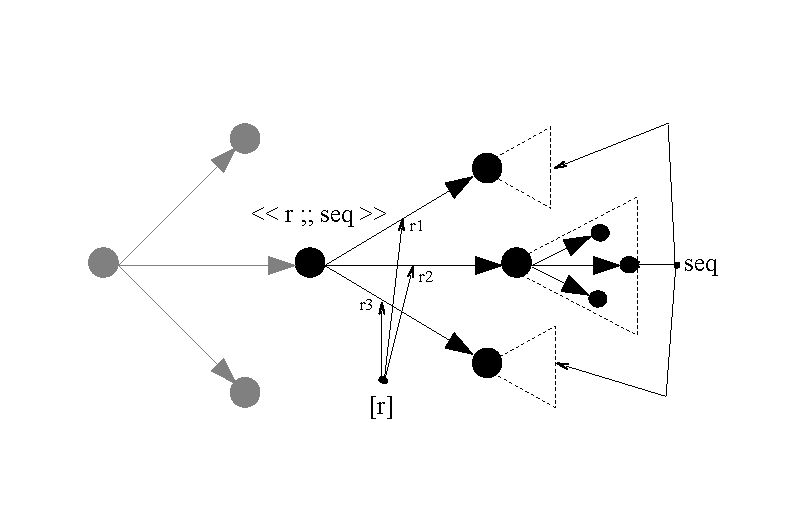
\includegraphics[width=\textwidth]{fig/SearchSpace}
  \caption{Search space illustration, a bullet stands for a graph}
  \label{figsearchspace}
\end{figure}

With each sequence call advancing one step into depth and each backtracking angle advancing into breadth, you receive a depth-first enumeration of an entire search space (as sketched in \ref{figsearchspace}).
Each state is visited in \emph{temporal succession}, with only the most recent state being available in the graph.
But maybe you want to keep each state visited, because you are interested in viewing all results at once, or because you want to compare the different states.
As there is only one host graph in \GrG, keeping each visited state requires a partition of the host graph into separate subgraphs, each denoting a state.

After you changed the modeling from a host graph to a state space graph consisting of multiple subgraphs, each representing one of the graphs you normally work with, 
you can materialize the search space visited in temporal succession into a state space graph,
by copying the subgraphs (which are normally only existing at one point in time) during \indexed{pause insertion}s out into space.
When subgraphs would be copied without pause insertions, they would be rolled back during backtracking; but effects applied on the graph from \texttt{/ in between here /} are bypassing the recording of the transaction undo log and thus stay in the graph, even if the transaction fails and is rolled back. 

When you have switched from a depth-first search over one single current graph to the unfolding of a state space graph containing all the subgraphs reached, you may compare each subgraph which gets enumerated with all the already available subgraphs, and if the new subgraph already exists (i.e. is isomorph to another already generated subgraph), you may refrain from inserting it.
This \indexed{symmetry reduction} allows to save the space and time needed for storing and computing equivalent branches otherwise generated from the equivalent states. 
But please note that the \texttt{==} operator on graphs is optimized for returning early when the graphs are different; when the graphs are isomorphic you have to pay the full price of graph isomorphy checking.
This will happen steadily with \indexed{automorphic pattern}s and then degrade performance.
To counter this filter the matches which cover the same spot in different ways, see \ref{sub:extflt} on how to do this.
Merging states with already computed ones yields a DAG-formed state space, instead of the always tree like search space.
Have a look at the transformation techniques chapter for more on state space enumeration \ref{sec:statespaceenum} and copying \ref{subsub:copystructure}.
One caveat of the transactions and backtracking must be mentioned: rollback might lead to an incorrect graph visualization when employed from the debugger.
This holds especially when using grouping nodes to visualize subgraph containment (\ref{sub:visual}). You must be aware that you can't rely on the online display as much as you can normally, and that you maybe need to fall back to an offline display by opening a \texttt{.vcg}-dump of the graph written in a situation when the online graph looked suspicious; a dump can be written easily in a situation of doubt from the debugger pressing the \texttt{p} key. 

\begin{note}
While a transaction or a backtrack is pending, all changes to the graph are recorded into some kind of undo log, which is used to reverse the effects on the graph in the case of rollback (and is thrown away when the nesting root gets committed).
So these constructs are not horribly inefficient, but they do have their price --- if you need them, use them, but evaluate first if you really do.
\end{note}


%%%%%%%%%%%%%%%%%%%%%%%%%%%%%%%%%%%%%%%%%%%%%%%%%%%%%%%%%%%%%%%%%%%%%%%%%%%%%%%%%%%%%%%%%%%%%%%%
\section{For Loops and Indeterministic Choice}

\begin{rail}
  ExtendedControl:
    'for' lbrace Variable ':' Type\\
    ('in' Function '(' Parameters ')' ';' |
    'in' '[' '?' r ']' ';')\\
    RewriteSequence rbrace
    ;
\end{rail}\ixkeyw{for}\label{forgraphelem}\label{forincidentadjacent}\label{formatch}

The \texttt{for} loop over the \emph{Functions} \texttt{nodes} or \texttt{edges} are iterating over all the elements in the current host graph which are compatible to the type given.
The iteration variable is bound to the currently enumerated graph element, then the sequence in the body is executed.

If you iterate a node type from a graph, you may be interested in iterating its incident edges or its adjacent nodes.
This can be achieved with a for neighbouring elements loop, which binds the iteration variable to an edge in case the \emph{Function} is one of \texttt{incoming}, \texttt{outgoing}, or \texttt{incident}. 
Or which binds the iteration variable to a node in case the \emph{Function} is one of \texttt{adjacentIncoming}, \texttt{adjacentOutgoing}, or \texttt{adjacent}.
Moreover, you may iterate with \texttt{reachableIncoming}, \texttt{reachableOutgoing}, and \texttt{reachable} the nodes reachable from a starting node, or with \texttt{reachableEdgesIncoming}, \texttt{reachableEdgesOutgoing}, and \texttt{reachableEdges} the edges reachable from a starting node.
The admissible \emph{Parameters} are the source node, or the source node plus the incident edge type, or the source node plus the incident edge type, plus the adjacent node type ---
that's the same as for the sequence expression functions explained in \ref{neighbouringelementsfunctions}/Connectedness queries.
In contrast to these set returning functions, this loop contained functions enumerate nodes/edges multiple times in case of reflexive or multi edges.

The third \texttt{for} loop introduced here, the for matches loop, allows to iterate through the matches found for an all-bracketed rule reduced to a test; i.e. the rule is not applied, we only iterate its matches.
The loop variable must be of a statically known \texttt{match<r>} type with \texttt{r} being the name of the rule matched.
The elements (esp. the nodes and edges) of the pattern of the matched rule can then be accessed by applying the \texttt{.}-operator on the loop variable, giving the name of the element of interest after the dot.
Note: the elements must be assigned to a variable in order to access their attributes, a direct attribute access after the match access is not possible.
Note: the match object allows only to access the top level nodes, edges, or variables.
If you use subpatterns or nested patterns and want to access elements found by them, you have to \texttt{yield}(\ref{sub:yield}) them out to the top-level pattern.

The most important \texttt{for} loop, the one iterating a container, for enumerating the elements contained in storages, was already introduced here: \ref{forstorage}.
All \texttt{for} loops fail if one of the sequence executions failed, and succeed otherwise.

\begin{rail}
  ExtendedControl:
		'highlight' '(' Arguments ')'
    ;
\end{rail}\ixkeyw{highlight}
The \texttt{highlight} sequence highlights the arguments given as a quoted text in the graph;
it does what the \texttt{(h)ighlight} command does in the debugger, see \ref{highlight}, just programmed from the sequences. 
Arguments is a comma-separated list of variable names or visited flag ids, the graph elements contained in the variables are highlighted, as are the graph elements marked by the visited flag.

\begin{rail} 
  ExtendedControl: 
	dollar (percent)? (ampersand | '|' | doubleampersand | '||') '(' SequencesList ')' |
	dollar (percent)? '.' '(' WeightedSequencesList ')' |
	(dollar (percent)? )? lbrace '<' ((RuleExecution)+(',')) '>' rbrace
	;
  SequencesList:
	RewriteSequence ((',' RewriteSequence)*())
	;
  WeightedSequencesList:
	WeightedSequence ((',' WeightedSequence)*())
	;
  WeightedSequence:
	FloatingNumber RewriteSequence
	;
\end{rail}\ixnterm{SequencesList}

The \indexed{indeterministic choice} operators execute chosen elements from a sets of rules or sequences.
The \indexed{random-all-of operators} given in function call notation with the dollar sign plus operator symbol as name have the following semantics:
The strict operators \verb/|/ and \verb/&/ evaluate all their subsequences in random order returning the disjunction resp. conjunction of their truth values.
The lazy operators \verb/||/ and \verb/&&/ evaluate the subsequences in random order as long as the outcome is not fixed or every subsequence was executed 
(which holds for the disjunction as long as there was no succeeding rule and for the conjunction as long as there was no failing rule).
A \indexed{choice point} may be used to define the subsequence to be executed next.

The \indexed{some-of-set braces} \verb/{(r,[s],$[t])}/ matches all contained rules and then executes the ones which matched.
The \indexed{one-of-set braces} \verb/${(r,[s],$[t])}/ (some-of-set with random choice applied) matches all contained rules and then executes at random one of the rules which matched
(i.e. the one match of a rule, all matches of an all bracketed rule, or one randomly chosen match of an all bracketed rule with random choice).
The one/some-of-set is true if at least one rule matched and false if no contained rule matched.
A \indexed{choice point} may be used on the one-of-set; it allows you to inspect the matches available graphically before deciding on the one to apply. 

The \indexed{weighted one operator} \verb/$.(w1 s1, ..., wn sn)/ is executed like this:
the weights \texttt{w1-wn} (numbers of type double) are added into a series of intervals,
then a random number (uniform distribution) is drawn in between \texttt{0.0} and \texttt{w1+...+wn},
the subsequence of the interval the number falls into is executed,
the result of the sequence is the result of the chosen subsequence.


%%%%%%%%%%%%%%%%%%%%%%%%%%%%%%%%%%%%%%%%%%%%%%%%%%%%%%%%%%%%%%%%%%%%%%%%%%%%%%%%%%%%%%%%%%%%%%%%
\section{Graph Nesting and Graph Oriented Programming}\label{sec:graphnesting}

Graph nesting is possible with nodes or edges of a graph bearing attributes of graph type (cf. \ref{cha:graph}).
They can then be filled with other graphs, employing the operations in \ref{sec:subgraphop}.

Attributes of graph type are opaque to the processing of the host graph containing them; 
their only direct usage is comparison, i.e. isomorphy checking against other graphs,
as needed for state space enumeration (cf. \ref{sec:statespaceenum}),
in this case only immutable subgraphs are stored.

\begin{rail} 
  ExtendedControl: 
    'in' (GraphVariable | NodeOrEdge '.' Attribute) lbrace RewriteSequence rbrace;
\end{rail}\ixkeyw{in}

But they can be opened up and made modifiable by switching the location of processing with the \verb#in g { seq }# sequence.
Inside the braces is the host graph switched to \texttt{g}, the sequence \texttt{seq} is executed in the host graph switched to, all queries and updates are carried out on the new graph; after executing the construct the old graph that was previously used is made the current host graph again.

\begin{rail}
  Rule: GraphVariable '.' RuleIdent (() | '(' (Variable+',') ')');
\end{rail}\ixnterm{Rule}

The rules are always applied on the current host graph without any ability to switch to a subgraph;
switching the location of processing is only available in the sequences.
But a simplified and more lightweight version of the full switch is available for single rule calls with \verb#g.r#; so a method call in the sequences denotes in fact a temporary subgraph switch.
To allow for this is the syntax of rule application extended by the grammar rule above.

The \emph{information hiding} shown by the graph attributes is comparable to the information hiding shown by the objects in \emph{object-oriented programming}, there the attributes but especially the neighbouring elements are only known to the containing object and accessible to the methods of the object.
In \emph{graph-oriented programming} are the attributes but especially the neighboring elements known to the containing graph, the connecting topology is open for \emph{pattern matching}.
This crucial difference also defines the main benefit compared to OO, removing it would mean to revert back to OO.
But this openness might not be needed always for all parts.
When building a \emph{large system}, you typically only need a certain \emph{layer} to be accessible at a time.
You may use graph attributes and nested graph in this case,
utilizing open graph-oriented programming for the parts you need to work globally with pattern matching at a time,
and closed object-oriented programming for parts you only need to access locally,
decoupled by explicit move-to-subgraph and return-to-subgraph steps.

You may model containment with edges denoting a containment type pointing to the contained parts instead of attributes of subgraph type
when the pattern matcher needs overall access to the graph, but there are still some containment or nesting relationships in place.
You can then still benefit from a hierarchical structure in debugging, utilizing the built-in nesting for visualization capabilities of \GrG (cf. \ref{sub:visual}, the graphs nested in attributes are truly opaque and invisible, only when processing switches to them are they displayed instead of their containing host graph).


%%%%%%%%%%%%%%%%%%%%%%%%%%%%%%%%%%%%%%%%%%%%%%%%%%%%%%%%%%%%%%%%%%%%%%%%%%%%%%%%%%%%%%%%%%%%%%%%
\section{Quick Reference Table}

Table~\ref{seqtab} lists most of the operations of the graph rewrite sequences at a glance.

%\makeatletter
\begin{table}[htbp]
\begin{minipage}{\linewidth} \renewcommand{\footnoterule}{} 
\begin{tabularx}{\linewidth}{|lX|}
\hline
\texttt{(w)=s(w)} & Calls a sequence \texttt{s} handing in \texttt{w} as input and writing its output to \texttt{w}; defined e.g. with \texttt{sequence s(u:Node):(v:Node)} \texttt{\{ v=u \}}.\\
\hline
\texttt{<s>}	& Execute \texttt{s} transactionally (rollback on failure).\\
\texttt{<<r;;s>>}	& Backtracking: try the matches of rule \texttt{r} until \texttt{s} succeeds.\\
\texttt{/ s /}	& Pause insertion: execute \texttt{s} outside of the enclosing transactions and sequences, i.e. the changes of \texttt{s} are not rolled back.\\
\hline
\texttt{highlight(vars)} & Highlights the content of the variables in the graph. \\
\hline
\texttt{\$\{<r1,[r2],\$[r3]>\}}	& Tries to match all contained rules, then rewrites indeterministically one of the rules which matched. True if at least one matched.\\
\hline
\texttt{for\{v in u; t\}}	& Execute \texttt{t} for every \texttt{v} in storage set \texttt{u}. One \texttt{t} failing pins the execution result to failure.\\
\texttt{for\{v->w in u; t\}}	& Execute \texttt{t} for every pair (\texttt{v},\texttt{w} in storage map \texttt{u}. One \texttt{t} failing pins the execution result to failure.\\
\texttt{for\{v:match<r> in [?r]; t\}}	& Execute \texttt{t} for every match \texttt{v} from rule \texttt{r}. One \texttt{t} failing pins the execution result to failure.\\
\texttt{for\{v:T; s\}}	& Execute \texttt{s} for every \texttt{v} of type \texttt{T} available in the graph. One \texttt{s} failing pins the execution result to failure.\\
\texttt{for\{v in func(w); s\}}	& Execute \texttt{s} for every edge/node incident/adjacent to \texttt{w} . One \texttt{s} failing pins the execution result to failure.\\
\hline
\texttt{in g \{s\}}	& Executes \texttt{s} in the graph \texttt{g}.\\
\hline
\texttt{\{comp\}}	& An unspecified sequence computation (see table \ref{comptab}).\\
\hline
\end{tabularx}\indexmain{\texttt{<>}}\indexmain{\texttt{<<;>>}}
\end{minipage}\\
\\ 
{\small Let \texttt{r}, \texttt{s}, \texttt{t} be sequences, \texttt{u}, \texttt{v}, \texttt{w} variable identifiers, \texttt{<op>} $\in \{\texttt{|}, \texttt{\textasciicircum}, \texttt{\&}, \texttt{||}, \texttt{\&\&}\}$ }%and \texttt{n}, \texttt{m} $\in \N_0$.}
\caption{Sequences at a glance}
\label{seqtab}
\end{table}
%\makeatother
 
% todo: beispiele im text bringen


\chapter{Transformation Techniques}\indexmain{imperativeandstate}
\label{cha:techniques}
\label{sub:mergesplit}

In this chapter we'll have a look at transformation techniques to solve common graph rewriting tasks utilizing the constructs introduces so far.
They could be offered directly by some dedicated operators,
but these would need so much customization to be useful in the different situations one needs them,
that we decided against dedicated operators;
instead it is on you to program the version you need yourself by \emph{combining} language constructs and rules.

The primary means to build transformations are top-level \emph{sequences}, controlling rule applications (on one or all matches).
They may call other sequences, even so recursively.
The sequences allow for \emph{external composition} of rules; a rule may be \emph{(re-)used} multiple times.
They follow the \emph{imperative} programming paradigm, one rule is applied after the other, on the \emph{then-changed} state (of the graph, changed after each step).

With \emph{embedded sequences} are you able to call rules from within a rule application, after the rule proper was executed (deferred execution), with direct access to the elements of that rule.
Seen from the outside, they allow to build a complex rule and thus allow for rule \emph{internal composition}, again in an \emph{imperative} way.
They allow to do work later on you can't do while executing the rule proper (e.g. because an element was already matched and is now locked due to the isomorphy constraint), to follow a breadth-splitting structure, or simply to split work into several parts, modularizing it, \emph{reusing} already available functionality.

The other means for \emph{internal composition} are the \emph{nested and subpatterns}.
They allow to match and rewrite complex patterns built in a structured way piece by piece.
With different pieces connected together, pieces to decide in between, and pieces which appear repeatedly.
They follow the \emph{functional} programming paradigm, a complex state change is built compositionally without graph changes in between, only after applying the rule in a big step is the graph changed (in fact after the rewriting half-step, following the matching half-step). 
They shift processing below the rules-combined-by-sequences level. 

The sequences typically use graph-element-valued variables to communicate a \emph{single spot} in the host graph that is currently getting processed in between the rules.
This can be generalized with \emph{storages (container variables)} capable of holding \emph{multiple spots}; they allow to store elements collected in one run and reuse them as input in another run (this is esp. useful if elements are reached on different paths).
You can break up a transformation into self-contained \emph{passes} mediated by some \emph{intermediate state} with those multi-valued variables. 

Besides, you can employ elementary procedures directly manipulating the graph and elementary functions directly querying the graph, combining them \emph{programmatically} with expressions and statements, abstracting them into own procedures and functions.
Those functions and procedures can then be \emph{used} from the \texttt{if} and \texttt{eval} parts of the rules, and from the sequences.

\begin{note}
Prefer declarative composition, it helps in keeping the code readable and easily adaptable.
Prefer internal embedding over external state passing, it is typically a good deal more concise.
But don't go to extremes regarding this, use the mode of composition that is suited to the task and feels best and most natural.

Avoid rules carrying out a tiny amount of work with a lot of input and output and heavy external orchestration (graph-rewriting,  assembler-level style), aim for a medium amount of work per rule call (well, normally more is better, but when you press too hard you can get over the top regarding understandability).
\end{note}

\begin{note}
An alternative to storage containment are visited flags, they allow to mark interesting elements directly.
The storage sets are more efficient compared to the visited flags in case the count of elements of interest is a good deal smaller than the number elements in the graph; they are looked up in the set, in contrast to the visited flags, which are used by enumerating all available graph elements, filtering according to the visited state.
The visited flags on the other hand are extremely memory efficient (for free as long as you use only a few of them at the same time).
\end{note}

\begin{note}
Don't forget the last resort if you must solve a task so complex that the above means of composition (regarding control-flow or data-flow) are not sufficient: adding helper nodes, edges, or attributes to the graph model and the graph itself, holding some intermediate state of processing. 
\end{note}

In the following we'll employ those constructs to merge and split nodes, emulate node replacement grammars, execute transformations in the narrow sense, aka mappings, copy substructures, compute flow equations over the graph structure with sets in the nodes, and enumerate state spaces.
Further examples can be found in \cite{CompilerOptimization} employing two storagesets switched in between for computing a wavefront running over a compiler graph and \cite{ProgramUnderstanding} using the nested and subpatterns for elegantly extracting a state machine model from a program graph.


\section{Merge and Split Nodes}\indexmain{merge node}\indexmain{split node}
Merging a node \texttt{m} into a node \texttt{n} means transferring all edges from node \texttt{m} to node \texttt{n}, then deleting node \texttt{m}.
Splitting a node \texttt{m} off from a node \texttt{n} means creating a node \texttt{m} and transferring some edges from node \texttt{n} to \texttt{m}.

In both cases there are a lot of different ways how to handle the operation exactly:
Maybe only incoming or only outgoing edges, or only edges of a certain type \texttt{T} or only edges not of type \texttt{T}; maybe the node \texttt{n} is to be retyped, maybe the edges are to be retyped.
But common is the transferring of edges; this can be handled succinctly by an \texttt{iterated} statement and the \texttt{copy} operator.
In case the node opposite to an edge may be incident to several such edges, one must use an \texttt{exec} instead (or the \texttt{independent} operator \ref{rule:homspec}), as every iteration locks the matched entities, so they can't get matched twice. Not needing the opposite node one could simply leave it unmentioned in the pattern, only referencing node \texttt{n} or \texttt{m} and the edge, but unfortunately we need the opposite node so we can connect the edge copy to it.

\begin{note}
In case a simple node merging without edge retyping is sufficient the retype'n'merge clause introduced in \ref{sec:merge} offers a much simpler alternative for merging.
\end{note}

Now we'll have a look at an example for node merging: T1-T2 analysis from compiler construction is used to find out whether a control flow graph of a subroutine is reducible, i.e. all loops are natural loops. All loops being natural loops is a very useful property for many analyses and optimizations. The analysis is split into two steps, T1 removes reflexive edges, T2 merges a control flow successor into its predecessor iff there is only one predecessor available. These two steps are iterated until the entire graph is collapsed into one node which means the control flow is reducible, or execution gets stuck before, in which case the control flow graph is irreducible.

The analysis is defined on simple graphs, i.e. if two control flow edges between two basic block nodes appear because of merging they are seen as one, i.e. they are automatically fused into one. As \GrG~is built on multigraphs we have to explicitly do the edge fusion in a further step T3.

First let us have a look at T1 and T3, which are rather boring ... ehm, straight forward:

  \begin{example}
    \begin{grgen}
rule T1 {
  n:BB -:cf-> n;

  replace {
    n; // delete relexive edges
  }
}
rule T3 {
  pred:BB -first:cf-> succ:BB;
  pred    -other:cf-> succ;

  modify { // kill multiedges
    delete(other);
  }
}
    \end{grgen}
  \end{example}

The interesting part is T2, this is the first version using an iterated statement:

  \begin{example}
    \begin{grgen}
rule T2 {
  pred:BB -e:cf-> succ:BB;
  negative {
    -e->;
    -:cf-> succ; // if succ has only one predecessor
  }
  iterated {
    succ -ee:cf-> n:BB;

    modify { // then merge succ into this predecessor
      pred -:copy<ee>-> n; // copying the succ edges to pred
    }
  }

  modify { // then merge succ into this predecessor
    delete(succ);
  }
}
    \end{grgen}
  \end{example}

In case a control flow graph would be a multi-graph, with several control flow edges between two nodes, one would have to use an \texttt{exec} with an all-bracketed rule instead of the \texttt{iterated}, to be able to match a multi-\texttt{cf}-edge target of \texttt{succ} multiple times (which is prevented in the \texttt{iterated} version by the isomorphy constraint locking the target after the first match).

This is the second version using exec instead, capable of handling multi edges:

  \begin{example}
    \begin{grgen}
rule T2exec
{
  pred:BB -e:cf-> succ:BB;
  negative {
    -e->;
    -:cf-> succ; // if succ has only one predecessor
  }

  modify { // then merge succ into this predecessor
    exec([copyToPred(pred, succ)] ;> delSucc(succ));
  }
}

rule copyToPred(pred:BB, succ:BB)
{
  succ -e:cf-> n:BB;

  modify {
    pred -:copy<e>-> n;
  }
}

rule delSucc(succ:BB)
{
  modify {
    delete(succ);
  }
}
    \end{grgen}
  \end{example}

Natural loops are so advantageous that one transforms irreducible graphs (which only occur by using wild gotos) into reducible ones, instead of bothering with them in the analyses and optimizations.
An irreducible graph can be made reducible by node splitting, which amounts to code duplication (in the program behind the control flow graph).
In a stuck situation after T1-T2 analysis, a \texttt{BB} node with multiple control flow predecessors is split into as many nodes as there are control flow predecessors, every one having the same control flow successors as the original node.
(Choosing the \texttt{cf} edges and \texttt{BB} nodes which yield the smallest amount of code duplication is another problem which we happily ignore here.)

  \begin{example}
We do the splitting by keeping the indeterministically chosen first cf edge, splitting off only further cf edges, replicating their common target.

    \begin{grgen}
rule split(succ:BB)
{
  pred:BB -first:cf-> succ;
  multiple {
    otherpred:BB -other:cf-> succ;

    modify {
      otherpred -newe:cf-> newsucc:copy<succ>;
      delete(other);
      exec(copyCfSuccFromTo(succ, newsucc));
    }
  }

  modify {
  }
}

rule copyCfSuccFromTo(pred:BB, newpred:BB)
{
  iterated {
    pred -e:cf-> succ:BB;

    modify {
      newpred -:copy<e>-> succ;
    }
  }

  modify {
  }
}
    \end{grgen}
  \end{example}

The examples given can be found in the \texttt{tests/mergeSplit/} directory including the control scripts and test graphs; you may add \texttt{debug} prefixes to the \texttt{exec} or \texttt{xgrs} statements in the graph rewrite script files and call GrShell with e.g. \texttt{mergeSplit/split.grs} as argument from the \texttt{tests} directory to watch execution.


\section{Node Replacement Grammars}\indexmain{node replacement grammar}\indexmainsee{edNCE}{node replacement grammar}
With node replacement grammars we mean edNCE grammars \cite{NodeReplacement}, which stands for edge label directed node controlled embedding. In this context free graph grammar formalism, every rule describes how a node with a nonterminal type is replaced by a subgraph containing terminal and nonterminal nodes and terminal edges. The nodes in the instantiated graph get connected to the nodes that were adjacent to the initial nonterminal node, by connection instructions which tell which edges of what direction and what type are to be created for which original edges of what direction and what type, going to a node of what type.

This kind of grammars can be encoded in \GrG~by rules with a left hand side consisting of a node with a type denoting a nonterminal and iterateds matching the edges and opposite nodes it is connected to of interest; "of interest" amounts to the type and direction of the edges and the type of the opposite node. The right hand side deletes the original node (thus implicitly the incident edges), creates the replacement subgraph, and tells in the rewrite part of the iterateds what new edges of what directedness and type are to be created, from the newly created nodes to the nodes adjacent to the original node. (Multiple edges between two nodes are not allowed in the node replacement formalism, in case you want to handle them you've to use \texttt{exec} as shown in the merge/split example above.)

The following example directly follows this encoding:

  \begin{example}
This is an example rule replacing a nonterminal node \texttt{n:NT} by a 3-clique.
For the outgoing \texttt{E1} edges of the original node, the new node \texttt{x} receives incoming \texttt{E2} edges.
And for incoming \texttt{E2} edges of the original node, the new nodes \texttt{y} and \texttt{z} receive edges of the same type, \texttt{y} with reversed direction and \texttt{z} of the exact dynamic subtype bearing the same values as the original edges.
    \begin{grgen}
rule example
{
  n:NT;

  iterated {
    n -:E1-> m:T;

    modify {
      x <-:E2- m;
    }
  }

  iterated {
    n <-e2:E2- m:T;

    modify {
      y -:E2-> m;
      z <-:copy<e2>- m;
    }
  }

  modify {
    delete(n);
    x:T -- y:T -- z:T -- x;
  }
}
    \end{grgen}
  \end{example}

As another example for node replacement grammars we encode the two rules needed for the generation of the completely connected graphs (cliques) in two \GrG~rules. The first replaces the nonterminal node by a new nonterminal node linked to a new terminal node, connecting both new nodes to all the nodes the original nonterminal node was adjacent to. The second replaces the nonterminal node by a terminal node, connecting the new terminal node to all the nodes the original nonterminal node was adjacent to. This "we want to preserve the original edges" can be handled more succinctly and efficiently by retyping which we gladly use instead of the iteration.

  \begin{example}
    \begin{grgen}
rule cliqueStep
{
  nt:NT;

  iterated {
    nt -- neighbour:T;

    modify {
      t -- neighbour;
      nnt -- neighbour;
    }
  }

  modify {
    delete(nt);
    t:T -- nnt:NT;
  }
}

rule cliqueTerminal
{
  nt:NT;

  modify {
    :T<nt>;
  }
}
    \end{grgen}
  \end{example}

The examples can be found in the \texttt{tests/nodeReplacementGrammar} directory.


\section{Mapping in a Rewriting Tool}\label{sec:transfo}\indexmain{transformation in a narrow sense}
\GrG{} is a \emph{rewrite} tool, i.e. you modify \emph{one} graph.
This is in contrast to \emph{transformation} or better \emph{mapping} tools, which are used for specifying mappings in between \emph{two} (or more) graphs. (Graphs are typically called models in this kind of tools. Don't confuse this with the notion of graph model in \GrG\ as introduced in chapter \ref{chapmodellang}. In model transformation parlance our graph model denotes a meta model, with a model adhering to a meta model, which in turn adheres to a meta meta model, climbing a ladder of bullshit abstraction leading right into the land of the hot-air merchants, eh..., the truthfully real software engineers. XML. Model. Meta. Meta-meta. Business-logic. Cloud. Bingo!))
The graph model might be a union of multiple graph models, and the graph may consist of multiple unconnected components, so you don't loose anything regarding expressiveness here.

What you loose is the automatic construction of the \indexed{traceability} links which allow to retrieve the source node from a mapped node or the mapped node from a source node, which is normally carried out by a mapping tool in the background.
And there are no built-in annotations by which you specify the model in which to match the elements.
But again neither means a loss in expressiveness.

You can construct the traceability links on your own.
Either by using simple edges between the nodes (this is not possible in a transformation tool as edges can only exist within a graph/model).
Or by using maps of node type to node type (or from edge type to edge type) which you must fill manually:
when you map a source node to a target node (i.e. for a matched source node you create a target node), you fill a global map from source to target nodes with this pair, and/or a global map from target to source nodes.
When you need this information, you look it up easily with \texttt{target=map[source]} or \texttt{source=map[target]}.
The highlight command \ref{tabdebug} of the debugger can visualize this storage map neatly by marking the contained nodes and adding directed edges in between the source and domain elements.
In some situations you are even better off: if the retype operator is sufficient, you can easily transform the graph in-place. A given, named graph element then denotes the source and the target, just at different points in time.

The lack of built-in model annotations can be overcome by several ways of partitioning the graph or its types. 
Often the types of the source and the target model are disjoint.
This is the most convenient case, as you save any extra notational effort, the types alone define the source and target.
If you experience name-clashes, because while being basically disjoint they use same names, 
you may use packages, to force disjointness for type names.
This comes at the price of always having to specify the meta-model, similar to how you specify the model in mapping tool.

In cases they are not disjoint but share certain parts/types,
you can tell the elements from different graphs apart by either using visited flags --- then each ``graph'' is marked to be visited with its own flag.
Or you may use anchor nodes representing subgraphs, with an edge from such an anchor node to all nodes contained in its subgraph.
Thus all nodes of a subgraph are adjacent to an anchor node, and the subgraph consists exactly of the induced subgraph of these adjacent nodes (see \ref{builtingraphcopying} for more on this kind of modelling).

So while you can write mapping (\emph{out-of-place}) transformations leaving the source untouched, do we recommend rewriting (\emph{in-place}) transformations (unless you have a strong real need for the former).
This of course and esp. holds for tasks that don't consist of mapping an entire representation into another one, completely changing its structure, but modifying an existing one (e.g. enriching it with additional information, or partial rewriting of constructs amenable to some kind of normalization, while keeping the rest simply intact).
Here you can simply leave the unchanged parts out, saving you from specification effort, and from execution time, because you don't need to copy the elements untouched during the transformation pass.
For simple mapping tasks you can employ relabeling as its concise rewriting alternative, for complex tasks that require a series of changes are you better off with rewriting due to the argument above, as only parts of each step/pass require a full change in structure.

Mapping \emph{tools} and languages are typically \emph{input-driven}, iterating the source model elements, to decide what target elements to produce from them (focusing one source element at a time, checking context conditions, to create a target pattern).
In rewrite tools you typically use a \emph{control program} that defines what is to be carried out, and commonly you work there \emph{output-driven}, calling rules that produce one target element, decided upon by querying the source model for the patterns that produce it (calling rules that rewrite into a target pattern from a complex source pattern matched).
This commonly results in a better understandable specification, showing an improved separation of concern.
With explicit control by the control program, you are free to choose how to drive the computation, adapting it to whatever suits the problem best.

\section{Comparing Structures}\label{subsub:comparestructure}\indexmain{subgraph comparison}\indexmainsee{compare structure}{subgraph comparison}
Structures are compared in three steps, the first is to collect all nodes of interest in a storage set, the second is to compute an induced subgraph from that set, and the third is to compare the subgraphs with the built-in graph comparison operators.

The first step typically consists of covering the nodes of the structure one wants to compare with iterated subpatterns,
i.e. subpatterns which match from a root node on with iterateds along the incident edges into breadth,
employing a subpattern again on the node adjacent to the root node to match into depth (see Fig. \ref{figspanningtree} for an illustration of how example \ref{graphcompex} matches the DAG reachable from the root node \verb#$1# on via outgoing edges).
In case the structure to compare consists of multiple connected components or is difficult to capture with iterated and subpatterns, you can collect it step by step with a sequence of rule applications building up the node set.

\begin{figure}[htbp]
  \centering
  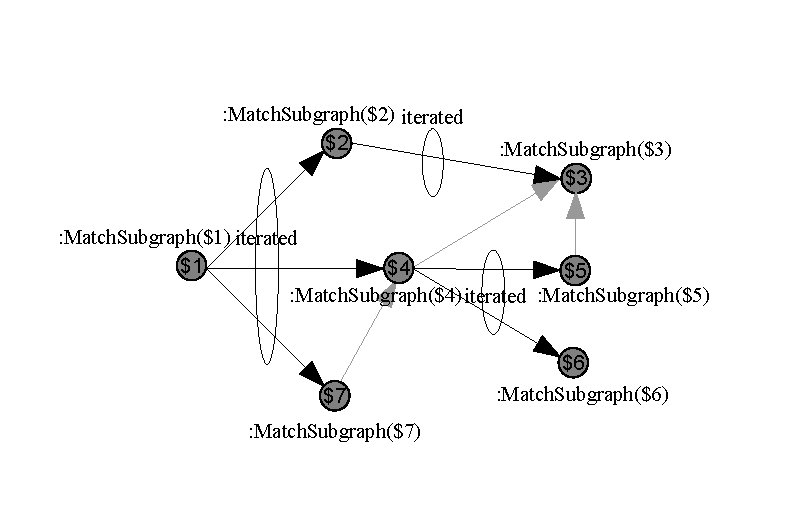
\includegraphics[width=\textwidth]{fig/SpanningTree}
  \caption{Matching a \indexed{spanning tree} in a graph}
  \label{figspanningtree}
\end{figure}

  \begin{example}\label{graphcompex}
    \begin{grgen}
pattern MatchSubgraph(root:Node, ref nodes:set<Node>)
{
  iterated { // match spanning tree of graph from root on
    root --> ch:Node;
    ms:MatchSubgraph(ch, nodes);

    modify {
      ms();
    }
  }

  modify {
    eval { nodes.add(root); } // build node set inducing graph
  }
}
    \end{grgen}
  \end{example}

The second step is to compute an induced subgraph from the node set collected, that can be done easily with the \texttt{inducedSubgraph} subgraph operation introduced in \ref{sec:subgraphop}:\\ \verb#exec sub:graph=inducedSubgraph(nodes)#.

The third step consists of comparing the subgraphs we filleted out of the common host graph with the graph comparison operators introduced in table \ref{compandgraph}:\\
\verb#exec if{sub1==sub2; doIso; doNonIso}#.

In case each such subgraph needs to be compared more than once it is recommended to add an attribute of type \texttt{graph} (see chapter \ref{cha:container}) to the subgraph starting anchor nodes, to assign the induced subgraph to this attribute, and to compare the subgraphs stored in these attribute.
This saves us the cost of computing the attributes and allows for further internal optimizations which 
may result in huge speedups.

\begin{warning}
The subgraph is not adapted automatically when the host graph changes, if this happens you must compute the stored subgraph anew manually.
\end{warning}

\noindent The comparison is then typically done with an idiom as such:\\
\verb#exec if{ for{other:AnchorNodeType; {curSub!=other.sub}} ; doNonIso(curSub)}# 
or such:\\
\verb#exec if{ for{other:graph in setOfCandidates; {curSub!=other}} ; doNonIso(curSub)}#.

Isomorphy comparison is an expensive operation, you can gain considerable speedups by using the parallelizable \texttt{equalsAny} function (cf. \ref{sec:subgraphop}) (and by specifying the number of worker threads (cf. \ref{sec:performanceparallel}), otherwise only a single one is used, saving you only the effort of manually coding the loop). 
In order to use this function you have to supply and maintain a set of the known subgraphs to check against in addition. 

\section{Copying Structures}\label{subsub:copystructure}\indexmain{subgraph copying}\indexmainsee{copy structure}{subgraph copying}
Structures are copied in two passes, the first consists of copying and collecting all nodes of interest, the second of copying all edges of interest in between the nodes.

The first pass consists of covering the nodes of the structure one wants to copy with iterated subpatterns,
in the same way as already introduced in \ref{subsub:comparestructure},
i.e. subpatterns which match from a root node on with iterateds along the incident edges into breadth,
employing a subpattern again on the node opposite to the root node to match into depth.
In the example we match the entire subgraph from a root node on, if one wants to copy a more constrained subgraph one can simple constrain the types, directions, and structures in the iterated subpattern covering the nodes.
The nodes are copied with the \texttt{copy} operators and a storagemap is filled, storing for every node copied its copy.

  \begin{example}
The example shows very generally how a subgraph reachable from a root node by incident edges can get copied, collecting and copying the nodes along a \indexed{spanning tree} from the root node on, then copying the edges in between the nodes in a second run afterwards. The edges get connected to the correct node copies via a mapping from the old to the new nodes remembered in a storage-map (\indexed{traceability} map).
    \begin{grgen}
pattern CopySubgraph(root:Node, ref oldToNew:map<Node, Node>)
{
  iterated { // match spanning tree of graph from root on
    root <--> ch:Node;
    cs:CopySubgraph(ch, oldToNew);

    modify {
      cs();
    }
  }

  modify {
    newroot:copy<root>; // copy nodes
    eval { oldToNew.add(root, newroot); }
    exec( [CopyOutgoingEdge(root, oldToNew)] ); // deferred copy edges
  }
}

rule CopyOutgoingEdge(n:Node, ref oldToNew:map<Node, Node>)
{
  n -e:Edge-> m:Node;
  hom(n,m); // reflexive edges
  nn:Node{oldToNew[n]}; nm:Node{oldToNew[m]};
  hom(nn,nm); // reflexive edges

  modify {
    nn -ee:copy<e>-> nm;
  }
}
    \end{grgen}
  \end{example}

The second pass is started after the structure matching ended by executing the deferred execs which were issued for every node handled.
Each \texttt{exec} copies all outgoing edges (one could process all incoming edges instead) of a node:
for each edge leaving the original node towards another original node a copy is created in between the copy of the original node and the copy of the other node.
The copies are looked up with the original nodes from the storage map (which fails for target nodes outside of the subgraph of interest).
Here too, one could constrain the subgraph copied by filtering certain edges.
In case of undirected edges one would have to prevent that edges get copied twice (once for every incident node). This would require a visited flag for marking the already copied edges or a storage receiving them, queried in the edge copying pattern and set/filled in the edge copying rewrite part.

The example can be found in the \texttt{tests/copyStructure} directory.
Without storagemaps one would have to pollute the graph model with helper edges linking the original to the copied nodes.

\subsection{Built-In Graph Copying}\label{builtingraphcopying}
In contrast to the just introduced general copying of an entire graph, you may choose a limited form of copying subgraphs.
This is enabled by the \texttt{insertInduced} and \texttt{insertDefined} operations introduced in \ref{sec:subgraphop}, which add a clone of the subgraph induced by the set of nodes or set of edges given as first argument to the host graph.
The clone of the second argument node or edge which was inserted into the host graph is returned as anchor element for further operations.

Before you can apply these operations you must collect the nodes or edges which are used to compute the induced subgraph.
Besides building the sets element-by-element with \texttt{add}-methods you may use set returning functions, e.g. \texttt{adjacent} introduced in \ref{neighbouringelementsfunctions}, which returns the set of all the nodes adjacent to the node given as (first) argument.

Employing \texttt{insertInduced(adjacent())} is a common idiom for copying a subgraph when the host graph is partitioned into multiple subgraphs in the following way:
a special node type \texttt{Graph} and a special edge type \texttt{contains} are introduced into the graph model. 
Every subgraph is represented by a \texttt{Graph} anchor node.
From these anchor nodes on \texttt{contains} edges lead to all the non-subgraph nodes contained in the corresponding subgraph.
With this modelling, all nodes in a subgraph are easily reachable from one anchor node via \texttt{adjacent}, and the entire subgraph can be easily retrieved by using \texttt{inducedSubgraph} or copied by \texttt{insertInduced}.
Besides this simplified manipulation, the graph can be easily visualized as being partitioned into multiple subgraphs with a \texttt{dump add node Graph group by contains} graph visualization command (see \ref{sub:visual} for more on this).


\section{Data Flow Analysis for Computing Reachability}\label{subsub:flow}\indexmain{flow equations}\indexmain{data flow analysis}\indexmain{reachability}
%todo: refine this nightly hacked section
%add dominance computation

In compiler construction, given a program graph, one wants to compute non-local properties in order to transform the program graph.
This is normally handled within the framework of data flow analysis, which employs flow equations telling how property values of a node are influenced by property values of the predecessor or successor nodes in addition to the node's local share on the overall information, with the predecessor or successor nodes being again influenced by their predecessor or successor nodes.
Property values are modeled as sets; the information is propagated around the graph until a fix point is reached (the operations must be monotone in order for a fix point to exist on the finite domain of discourse).
You might be interested in the transparencies under \url{http://www.imm.dtu.dk/~hrni/PPA/slides2.pdf} for some reading on this topic;
especially as this is a general method to compute non-local informations over graphs not limited to compiler construction.

We'll apply a backward may analysis (with only $gen$ but no $kill$ information) to compute for each node the nodes which can be reached from this node.
Reachability is an interesting property if you have to do a lot of iterated path checks:
instead of computing the itererated path with a recursive pattern each and every time you must check for it,
compute it once and just look it up from then on.
If you need to check several paths which must be disjoint you won't get around employing recursive subpatterns with one locking the elements for the other; but even in this case the precomputed information should be valuable (unless the graph is heavily connected), constraining the search to source and target nodes between which a path does exist, eliminating nodes which are not connected.

The reachability information will be stored in a storage set per node of the graph (indeed, we trade memory space for execution speed):
  \begin{example}
    \begin{grgen}
node class N
{
	reachable:set<N>;
}
    \end{grgen}
  \end{example}

The analysis begins with initializing all the storage sets with the local information about the direct successors by employing the following rule on all possible matches:
  \begin{example}
    \begin{grgen}
rule directReachability
{
  hom(n,m);
  n:N --> m:N;

  modify {
    eval { n.reachable.add(m); }
  }
}
    \end{grgen}
  \end{example}

The analysis works by keeping a global todo-set \verb#todo# containing all the nodes which need to be (re-)visited,
because the information in one of their successors changed;
this set is initialized with all nodes available using the sequence \verb#[addAllNodesToWorkset(todo)]#).

From then on in each iteration step a node \verb#n# is removed with \verb#(n)=pickAndRemove(todo)#, until the todo-set becomes empty, signaling the termination of the analysis; the node is processed by determining its successors \verb#[successors(n, succs)]#, adding the reachability information available in each successor to \verb#n# controlled by the sequence\\
\verb#for{s in succs; (changed)=propagateBackwards(n,s,changed)}#.\\
If the information in \verb#n# changed due to this, the predecessors of the node are added to the workset via \verb#if{changed;[addPredecessors(n,todo)]}#.

  \begin{example}
This is the core rule of the dataflow analysis: the reachability information from the successor node \texttt{s} in its \texttt{reachable} storage attribute is added to the storage attribute of the node \texttt{n} of interest; if the storage set changes this is written to the returned variable.
    \begin{grgen}
rule propagateBackwards(n:N, s:N, var changed:boolean) : (boolean)
{
  modify {
    eval { n.reachable |= s.reachable |> changed; }
    return(changed);
  }
}
    \end{grgen}
  \end{example}

The example can be found in the \texttt{tests/dataFlowAnalysis} directory, just add \texttt{debug} before the \texttt{exec} (or \texttt{xgrs}) in \texttt{dataFlowAnalysisForReachability.grs} and watch it run.
A sample situation showing a propagation step is given in \ref{figdataflow}.
The subgraph at the top-left is already handled as you can see by the reachable set displayed in each node.

\begin{figure}[htbp]
  \centering
  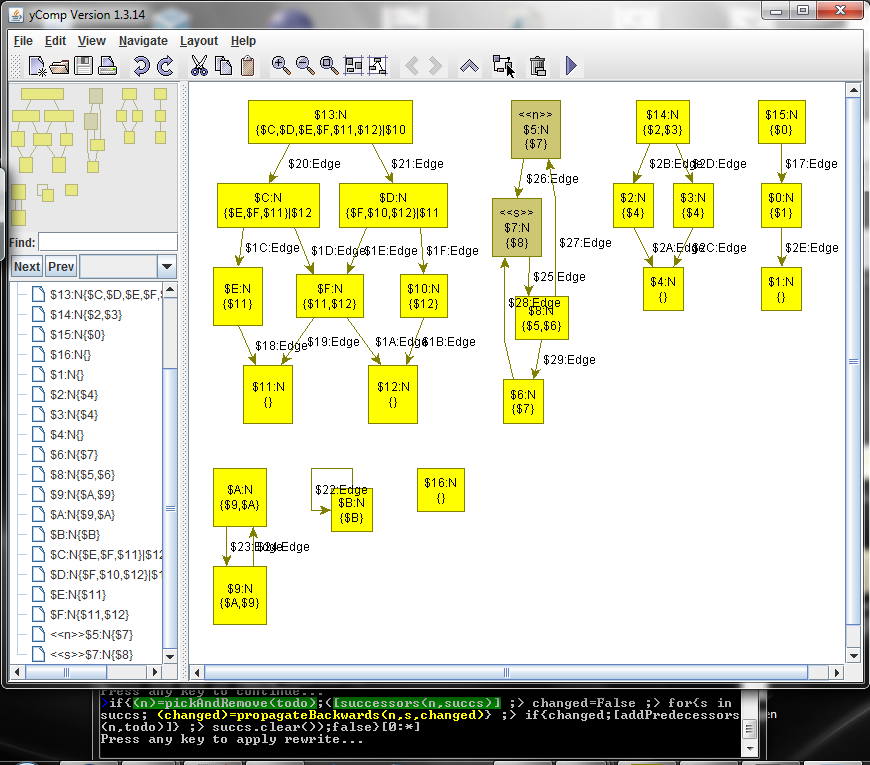
\includegraphics[width=\textwidth]{fig/Dataflow}
  \caption{Situation from dataflow analysis}
  \label{figdataflow}
\end{figure}

\subsubsection*{Worklist Based Data Flow Analysis}\indexmain{worklist}

The approach introduced above implements the basics but will not scale well to large graphs -- even medium sized graphs -- due to the random order the nodes are visited.
What is used in practice instead is a version employing a worklist built in postorder, so that a node is only visited after all its successor nodes have been processed.
For graphs without backedges, i.e. loops for program graphs, this gives an analysis which visits every node exactly once in the propagation phase.
For graphs with loops some nodes will be visited multiple times, but due to the ordering the analysis still terminates very fast.

The worklist is implemented directly in the graph by additional edges of the special type \verb#then# between the nodes, and a special node for the list start; the \verb#todo# set is kept, to allow for a fast "is the node already contained in the worklist"-check, used to save us from adding nodes again which are already contained (thus will be visited in the future anyway); i.e. the abstract worklist concept is implemented by the todo-set and the list added invasively to the graph.

  \begin{example}
    \begin{grgen}
edge class then; // for building worklist of nodes to be handled
    \end{grgen}
  \end{example}

\noindent The initial todo-set population of the simple approach is replaced by worklist constructing, successively advancing the last node of the worklist given by the \verb#last# variable; it starts with all nodes having no successor:\\
\verb#(last)=addFinalNodesToWorklist(last, todo)*#\\
Then iteratively all nodes which lead to them get added:\\
\verb#( (last)=addFurther(pos, last, todo)* ;> (pos)=switchToNextWorklistPosition(pos) )*#\\
In case of loops without terminal nodes we pick an arbitrary node from them:\\ \verb#(last)=addNotYetVisitedNodeToWorklist(last, todo)#\\
and add everything what leads to them, until every node was added to the worklist.

Now we can start the analysis, which works like the simple one does, utilizing the very same propagation rule,but follows the worklist instead of randomly picking from a todo-set, shrinking and growing the worklist along the way.

  \begin{example}
An example rule for worklist handling, adding a not yet contained node to the worklist; please note the quick check for containment via the set membership query.
    \begin{grgen}
rule addToWorklist(p:N, ref todo:set<N>, last:N) : (N)
{
  if{ !(p in todo); }

  modify {
    last -:then-> p;
    eval { todo.add(p); }
    return(p);
  }
}
    \end{grgen}
  \end{example}

  \begin{example}
An exmaple rule for worklist handling, removing the by-then processed node \texttt{pos} from the worklist.
    \begin{grgen}
rule nextWorklistPosition(pos:N, ref todo:set<N>) : (N)
{
  pos -t:then-> next:N;

  modify {
    delete(t);
    eval { todo.rem(pos); }
    return(next);
  }
}
    \end{grgen}
  \end{example}

The example can be found in the \texttt{tests/dataFlowAnalysis} directory, just add \texttt{debug} before the \texttt{exec} (or \texttt{xgrs}) in \texttt{dataFlowAnalysisForReachabilityWorklist.grs} and watch it run.
A sample situation showing a worklist building step is given in \ref{figworklist}.
The subgraph at the top-left is already handled as you can see by the reachable set displayed in each node.

\begin{figure}[htbp]
  \centering
  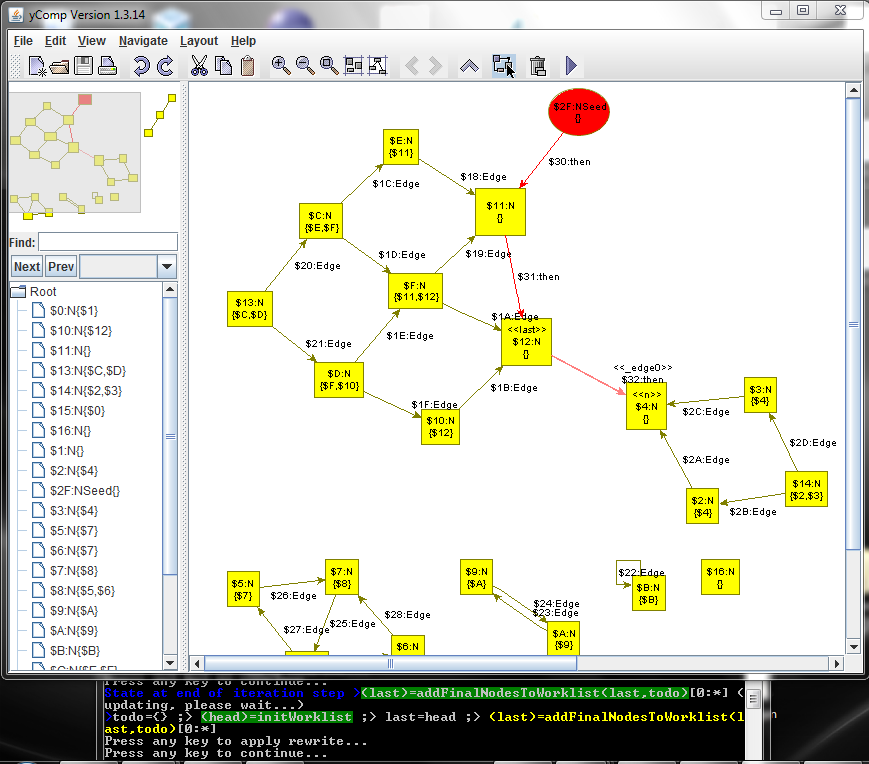
\includegraphics[width=\textwidth]{fig/Worklist}
  \caption{Situation from worklist building}
  \label{figworklist}
\end{figure}


\section{State Space Enumeration}\label{sec:statespaceenum}\indexmain{state space enumeration}
%todo: extend, refine this quick-hacked text

State space enumeration can be programmed in GrGen.NET utilizing the sequence constructs introduced up so far.
GrGen.NET always operates on one host graph, over one combined model, applying actions from one combined rule set --- so everything is always within reach.
That is by far the most simple approach to graph transformation, and for a tool which is not specially geared towards enumerating state spaces what makes most sense.
Thus state space enumeration (or transformation between different graphs/models) must be realized within the one host graph.
This can be achieved by virtually partitioning the host graph into smaller graphs or subgraphs, following a convention like this one:
There are nodes of type \texttt{Graph} which are representing a state of the statespace; each such representative is an anchor node for a subgraph.
The containment in the subgraph is denoted by a \texttt{contains} edge from a node of type \texttt{Graph} to all the nodes contained in this (sub)graph.
The edges between the \texttt{Graph} nodes give the relationship between the subgraphs, i.e. successorship between the states of the statespace.
The edges between the non-\texttt{Graph} nodes are the "normal" graph edges inside the subgraphs.

The key ingredients for state space enumeration then are
\begin{itemize}
	\item The aforementioned modelling with anchor nodes linking to the subgraphs, i.e. states
	\item Backtracking angles --- they allow to recursively enumerate and apply the matches of a rule found, exhaustively stepping through the state space, rolling back the effects on the graph of the previous match tried before carrying out the next step (see section \ref{sec:extctrl})
	\item Pause insertions --- they allow to write the interesting subgraphs found during state space search out into the host graph while effects recording of backtracking supervision is paused, so that they are not rolled back during backtracking (see section \ref{sec:extctrl})
	\item Recursive sequences --- they allow to nest backtracking angles dynamically, so it becomes possible to enumerate an entire state space with a sequence just implementing one backtracking step (see section \ref{sec:sequencedefinition})
	\item The capability to create a copy of a subgraph and insert it into the host graph (see section \ref{subsub:copystructure}, esp. subsection \ref{builtingraphcopying})
	\item The ability to compare subgraphs (see section \ref{subsub:comparestructure}).
Implemented in an optimized way with a subgraph attribute in the anchor nodes which contains a copy of the subgraph in the host graph, ready to be compared to the current graph, in order to decide whether that one should be inserted into the state space or purged for being an isomorphic copy of an already available instance. Potentially even further improved with an additional set of subgraphs, compared against with the parallelizable \texttt{equalsAny} function.
	\item Adjacency and induced functions to compute the subgraphs from the host graph following the \texttt{contains} edges from the anchor nodes (see section \ref{neighbouringelementsfunctions}, Connectedness Queries and section \ref{sec:subgraphop}, Subgraph Operations)
	\item The \texttt{auto} filters from \ref{sub:extflt} finally allow to optimize performance by filtering symmetric matches stemming from automorphic patterns. This is a lot more efficient than creating states which are for sure isomorphic and filtering them later on by comparison with all the other states.
\end{itemize}

The modelling given above allows to employ the ability of GrGen.NET/yComp to visualize nested graphs from a flat graph by interpreting node containment along edges of a special type (cf. \ref{sub:visual}), ballooning the anchor node up to a subgraph. 

An example implementation of this approach with a variant utilizing isomorphy checking and a variant without isomorphy checking can be found in the \texttt{tests/statespace} folder.
Feel free to drop in some \texttt{debug} prefixes before the \texttt{exec} (/\texttt{xgrs}) used to watch the assembling of the state space graph.
Another example implementation can be found in the \texttt{tests/statespaceChemistry} folder.
It shows how to enumerate all possible reaction results derivable from a set of start molecules according to some reaction rules.
The molecules are just accumulated in the host graph, it is taken care by storage sets that each step only processes the ones available at the start of the step.
At the end, each resulting molecule (i.e. connected component) is exported as a \texttt{.grsi} file.



\chapter{GrShell Language}\indexmain{GrShell}
\label{chapgrshell}
\GrShell\ is a \indexedsee{shell}{GrShell} application built on top of \LibGr\indexmain{libGr}. 
It belongs to \GrG's standard equipment. 
\GrShell\ is capable of creating, manipulating, and dumping graphs as well as performing and debugging graph rewriting.
The \GrShell\ provides a line oriented scripting language. 
\GrShell\ scripts are structured by simple statements separated by line breaks.

%rewrite stuff to be command based insteaf of splitting commands over several sections?

\section{Building Blocks}

\GrShell\ is \indexed{case sensitive}. 
A line may be emty, may contain a shell command, or may contain a comment. 
A \indexed{comment} starts with a \indexed{\texttt{\#}} and is terminated by end-of-line or end-of-file. 
The following items are required for representing text, numbers, and rule parameters.\\
\\
\emph{Text}\\
May be one of the following:
\begin{itemize}
  \item A non-empty character sequence consisting of letters, digits, and underscores. The first character must not be a digit.
  \item Arbitrary text enclosed by double quotes (\texttt{""}).
  \item Arbitrary text enclosed by single quotes (\texttt{''}).
\end{itemize}
\mbox{ }\\
\emph{Number}\\
Is an \texttt{int} or \texttt{float} constant in decimal notation (see also Section~\ref{builtin}).

\begin{rail} 
 Parameters : Text + ',' ;
 SpacedParameters: Text + ; 
\end{rail}\ixnterm{Parameters}\ixnterm{SpacedParameters}

In order to describe the commands more precisely, the following (semantic) specializations of \emph{Text} are defined:
\begin{description}
  \item[Filename]A fully qualified file name without spaces (e.g.\ \texttt{/Users/Bob/amazing\textunderscore file.txt}) or a single quoted or double quoted fully qualified file name that may contain spaces (\texttt{"/Users/Bob/amazing file.txt"}).
  \item[Variable] Identifier of a variable that contains a graph element or a value of basic type. 
  \item[NodeType, EdgeType] Identifier of a node type resp.\ edge type defined in the model of the current graph.
  \item[AttributeName] Identifier of an attribute.
  \item[Graph] Identifies a graph by its name.
  \item[Action] Identifies a rule by its name.
  \item[Color] One of the following \indexed{color} identifiers: \texttt{Black}, \texttt{Blue}, \texttt{Green}, \texttt{Cyan}, \texttt{Red}, \texttt{Purple}, \texttt{Brown}, \texttt{Grey}, \texttt{LightGrey}, \texttt{LightBlue}, \texttt{LightGreen}, \texttt{LightCyan}, \texttt{LightRed}, \texttt{LightPurple}, \texttt{Yel\-low}, \texttt{White}, \texttt{DarkBlue}, \texttt{DarkRed}, \texttt{DarkGreen}, \texttt{DarkYellow}, \texttt{DarkMagenta}, \texttt{DarkCyan}, \texttt{Gold}, \texttt{Lilac}, \texttt{Turquoise}, \texttt{Aquamarine}, \texttt{Khaki}, \texttt{Pink}, \texttt{Orange}, \texttt{Orchid}. These are the same color identifiers as in \indexed{VCG}/\yComp\ files (for a VCG definition see~\cite{vcg}).
\end{description}
\makeatletter
\begin{rail}
  GraphElement: Text | ('@' '(' Text ')')
\end{rail}\indexmain{\texttt{"@}}\ixnterm{GraphElement}
\makeatother
The elements of a graph (nodes and edges) can be accessed both by their \indexed{variable} identifier and by their \newterm{persistent name} specified through a constructor (see Section~\ref{mani}).
The specializations \emph{Node} and \emph{Edge} of \emph{GraphElement} require the corresponding graph element to be a node or an edge respectively.
\begin{example}
\label{persistentex} 
We insert a node, \indexed{anonymous}ly and with a \indexed{constructor} (see also Section~\ref{mani}):
\begin{grshell}
> new graph "../lib/lgsp-TuringModel.dll" G
New graph "G" of model "Turing" created.
  
# insert an anonymous node... 
# it will get a persistent pseudo name
> new :State  
New node "$0" of type "State" has been created.
> delete node @("$0")
  
# and now with constructor
> new v:State($=start) 
new node "start" of type "State" has been created.
# Now we have a node named "start" and a variable v assigned to "start"
\end{grshell}
\end{example}
\begin{note}
Persistent names will be saved (\texttt{save graph\dots}, see Section~\ref{outputcmds}) and exported, and, if you visualize a graph (\texttt{dump graph\dots}, see Section~\ref{outputcmds}), graph elements will be \indexed{label}ed with their persistent names.
Persistent names have to be unique for a graph (the graph they belong to).
\end{note}

\begin{rail}
  Variable '=' ( GraphElement | Variable | Literal )
\end{rail}
Assigns the variable or persistent name \emph{GraphElement} or literal to \emph{Variable}. If \emph{Variable} has not been defined yet, it will be defined implicitly. As usual for scripting languages, variables have neither static types nor declarations.

\begin{rail} 
'show' 'var' Variable 
\end{rail}\ixkeyw{show}
Prints the content of the specified variable.


\section{\GrShell\ Commands}
This section describes the \GrShell\ commands\ixnterm{Command}. Commands are assembled from basic elements. 
As stated before commands are terminated by line breaks. Alternatively commands can be terminated by the \indexed{\texttt{;;}} symbol.
Like an operating system shell, the \GrShell\ allows you to span a single command over $n$ lines by terminating the first $n-1$ lines with a \indexed{backslash}.  
\begin{rail}
  Script: ((Command ('<line break>' | ';;'))+) '<end of file>' ;
\end{rail}\ixnterm{Script}


\subsection{Common Commands}
\label{commcommands}
\begin{rail}
  'help' (Command)?
\end{rail}\ixkeyw{help}
Displays an information message describing all the supported commands. 
A command \texttt{Command} displayed with \texttt{...} has further help available, which can be displayed with \texttt{help Command}.

\begin{rail}
  'quit' | 'exit'
\end{rail}\ixkeyw{quit}\ixkeyw{exit}
Quits \GrShell. If \GrShell\ is opened in debug mode, a currently active graph viewer (such as \yComp) will be closed as well.

\begin{rail}
  'include' Filename
\end{rail}\ixkeyw{include}
Executes the \GrShell\ script\indexmain{graph rewrite script} \emph{Filename}.
A \GrShell\ script is just a plain text file containing \GrShell\ commands.
They are treated as they would be entered interactively, except for parser error
If a parser error occurs, execution of the script will stop immediately.

\begin{rail}
  'echo' Text
\end{rail}\ixkeyw{echo}
Prints \emph{Text} onto the \GrShell\ command prompt.

\begin{rail}
  '!' CommandLine
\end{rail}\indexmain{\texttt{"!}}
\emph{CommandLine}\indexmain{command line} is an arbitrary text, the operating system attempts to execute.
\begin{example}
On a Linux machine you might execute
\begin{grshell}
!sh -c "ls | grep stuff"
\end{grshell}
\end{example}

\begin{rail}
'silence' ('on'|'off')
\end{rail}\ixkeyw{silence}
Switches the new node / edge created / deleted messages on(default) or off.
Switching them off allows for much faster execution of scripts containing a lot of creation commands.

\begin{rail}
'randomseed' (Number | 'time')
\end{rail}\ixkeyw{randomseed}
Sets the random seed to the given number for reproducible results when using the \$-operator-prefix or the random-match-selector, whereas time sets the random seed to the current time in ms.

\begin{rail}
'redirect' 'emit' Filename
\end{rail}\ixkeyw{redirect}\ixkeyw{emit}
Redirects the output of the emit-statements in the rules from stdout to the given file.

\begin{rail}
'redirect' 'emit' '-'
\end{rail}\ixkeyw{redirect}\ixkeyw{emit}
Redirects the output of the emit-statements in the rules to stdout (again).


\subsection{Graph Commands}
\label{graphcommands}

\begin{rail}
  'new' 'graph' Filename Text 
\end{rail}\ixkeyw{new}\ixkeyw{graph}
Creates a new graph with the model specified in \emph{Filename}\indexmain{graph model}.
Its name is set to \emph{Text}. 
The model file can be either source code (e.g.\ \texttt{turing\textunderscore machineModel.cs}) or a .NET assembly (e.g.\ \texttt{lgsp-turing\textunderscore machineModel.dll}).
It's also possible to specify a rule set file as \emph{Filename}. 
In this case the necessary assemblies will be created on the fly.

\begin{rail}
  'open' 'graph' Filename Text
\end{rail}\ixkeyw{open}\ixkeyw{graph}
Opens the graph \emph{Text} stored in the backend. 
However, the \emph{LGSPBackend} doesn't support \indexed{persistent graph}s, and as the \emph{LGSPBackend} is the only backend available at the moment, this command is currently useless.
You may achieve persistence by using import/export or save/include instead.

\begin{rail}
  'show' 'graphs'
\end{rail}\ixkeyw{show}\ixkeyw{graph}
Displays a list of currently available graphs.

\begin{rail}
  'select' 'graph' Graph
\end{rail}\ixkeyw{select}\ixkeyw{graph}
Selects the current \indexed{working graph}.
This graph acts as \emph{\indexed{host graph}} for graph rewrite sequences (see also Sections~\ref{ov:whatsallabout} and~\ref{grsthings}).
Though you can define multiple graphs, only one graph can be the active ``working graph''.

\begin{rail}
  'clear' 'graph' (() | Graph)
\end{rail}\ixkeyw{clear}\ixkeyw{graph}
Deletes all graph elements of the current working graph resp.\ the graph \emph{Graph}.

\begin{rail}
  'delete' 'graph' Graph
\end{rail}\ixkeyw{delete}\ixkeyw{graph}
Deletes the graph \emph{Graph} from the backend storage.


\subsection{Validation Commands}

\GrG\ offers two different graph validation mechanisms, the first checks against the connection assertions specified in the model, the second checks against an arbitrary graph rewrite sequence containing arbitrary tests and rules.

\begin{rail}
  'validate' ('exitonfailure')? ('strict')?
\end{rail}\ixkeyw{validate}\ixkeyw{strict}
Validates\indexmain{validate} if the current working graph fulfills the \indexed{connection assertion}s specified in the corresponding graph model.
The \emph{strict} mode additionally requires all the edges available in the instance graph to be specified in the model in order to be ``valid''.
Otherwise edges between nodes without specified constraints are ignored.
The \texttt{validate xgrs} version checks if the graph fullfills the given graph rewrite sequence.
Validation fails iff the xgrs fails, thus giving a very flexible and powerful mechanism to specify graph constraints.
The GrShell is exited with an error code if \texttt{exitonfailure} is specified and the validation fails.

\begin{example}
We reuse a simplified version of the road map model from chapter~\ref{chapmodellang}:
\begin{grgen} 
model Map;

node class city;
node class metropolis;

edge class street;
edge class highway
      connect metropolis [+] -> metropolis [+];
\end{grgen}
The node constraint on \emph{highway} requires all the metropolises to be connected by highways. Now have a look at the following graph:
\begin{center}
  \fbox{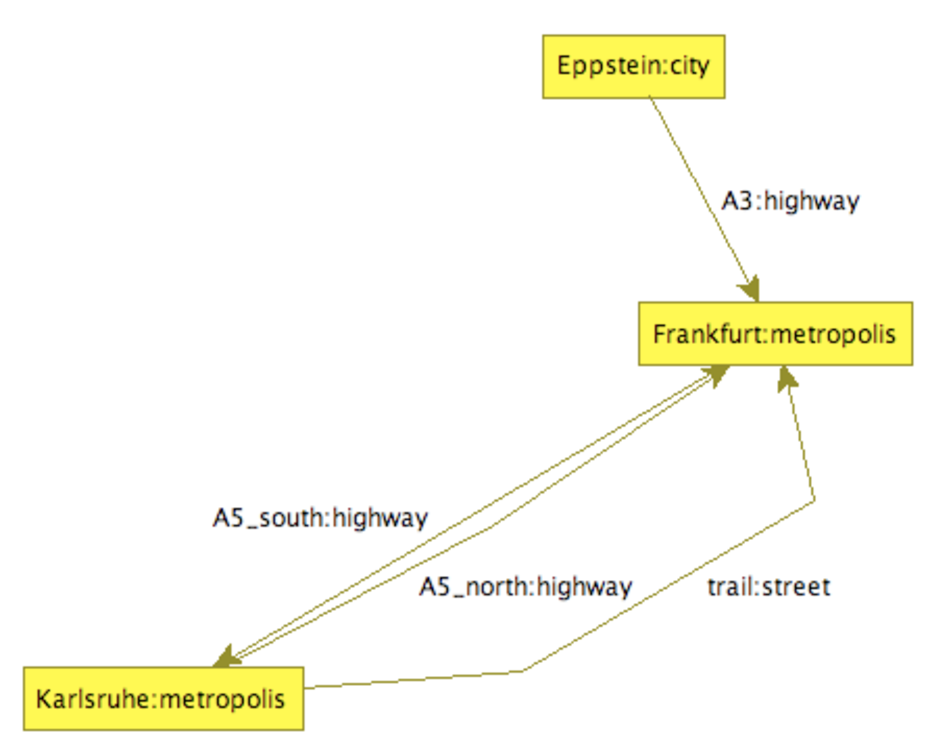
\includegraphics[width=8.5cm]{fig/map}}
\end{center}

This graph is valid but not strict valid.
\begin{grshell} 
> validate
The graph is valid.
> validate strict
The graph is NOT valid:
  CAE: city "Eppstein" -- highway "A3" --> metropolis "Frankfurt" not specified
  CAE: metropolis "Karlsruhe" -- street "trail" --> metropolis "Frankfurt" not specified
>
\end{grshell}
\end{example}

\begin{rail}
  'validate' ('exitonfailure')? 'xgrs' GRS
\end{rail}\ixkeyw{validate}\ixkeyw{grs}
Validates\indexmain{validate} if the current working graph satisfies the \indexed{graph rewrite sequence} given.
Before the graph rewrite sequence is executed, the instance graph gets cloned;
the sequence operates on the clone, allowing you to change the graph as you want to, without influence on the host graph.
Validation fails iff the xgrs fails.
This gives a rather costly but extremely flexible and powerful mechanism to specify graph constraints.
The GrShell is exited with an error code if \texttt{exitonfailure} is specified and the validation fails.


\subsection{Visited Flag Commands}

\begin{rail}
'Variable' '=' 'allocvisitflag'
\end{rail}\ixkeyw{allocvisitflag}\label{allocvisitflag}
Allocates space for a visited flag in the elements of the graph and returns the id of the visited flag (integer number), starting at 0.
Afterwards, the visited flag of the id can be read and written within the rules by the \texttt{visited}-expression and the \texttt{visited}-assignment,
as well as by the \texttt{isvisited} and \texttt{setvisited} shell commands.
The first visited flags are stored in some excess bytes of the graph elements and are thus essentially for free, but if this implementation defined space is used up completely, the information is stored in dictionaries.

\begin{rail}
'freevisitflag' 'Variable'
\end{rail}\ixkeyw{freevisitflag}
Frees the space previously allocated for the visited flag; afterwards you must not access it anymore. 
The value stored in the variable must be of integer type, stemming from a previous allocation.

\begin{rail} 
'setvisited' GraphElement 'flagId' 'BooleanValue'
\end{rail}\ixkeyw{setvisited}
Sets the visited status of the graph element of the flag id the given boolean value; visited flags are normally written by rules of the rule language.

\begin{rail}
'isvisited' GraphElement 'flagId'
\end{rail}\ixkeyw{isvisited}
Returns the visited status of the graph element of the flag id; visited flags are normally read by tests and rules of the rule language.


\subsection{Graph Input and Output Commands}
\label{outputcmds}

\begin{rail}
  'save' 'graph' Filename
\end{rail}\ixkeyw{save}\ixkeyw{graph}
Dumps\indexmain{dumping graph} the current graph as \GrShell\ script\indexmain{graph rewrite script} into \emph{Filename}.
The created script includes
\begin{itemize}
  \item selecting the backend
  \item creating a new graph with all nodes and edges (including their persistent names)
  \item restoring the variables
  \item restoring the visualisation styles
\end{itemize}
but not necessarily using the same commands you typed in during construction. 
Such a script can be loaded and executed by the \texttt{include} command (see Section~\ref{commcommands}).

\begin{rail}
  'export' Filename.grs (withvariables)?
\end{rail}\ixkeyw{export}
Exports an instance graph in GRS format, which is a reduced \GrShell\ script (it can get imported and exported on API level\ref{sub:imexport} without using the \GrShell\).
It contains the \texttt{new graph} command, followed by \texttt{new node} commands, followed by \texttt{new edge} commands.
If \texttt{withvariables} is specified, the variables are exported, too.
The export is only complete with the model of the graph given in the \texttt{.gm} file.
Exporting fails if the graph model contains attributes of \texttt{object}-type.
The \texttt{save} command is for saving a \GrShell\ session including visualization styles, the goal of the \texttt{export} command is graph rewrite system interoperability.

\begin{rail}
  'export' Filename.gxl
\end{rail}\ixkeyw{export}
Exports an instance graph and a graph model in GXL format \ref{}, which is somewhat of a standard format for graphs of graph rewrite systems, but suffers from the well-known XML problems -- it is barely human-readable and bloated.
Exporting fails if the graph model contains attributes of \texttt{set<S>}-,\texttt{map<S,T>}-, or \texttt{object}-type.

\begin{rail}
  'import' Filename.grs
\end{rail}\ixkeyw{import}
Imports the specified graph instance in GRS format (the \emph{reduced} \GrShell\ script, a saved graph can only be imported by \texttt{include} (but an exported graph can be imported by \texttt{include}, too)).
The referenced graph model must be available as \texttt{.gm}-file.

\begin{rail}
  'import' Filename.gxl (ModelOverride)?
\end{rail}\ixkeyw{import}
Imports the specified graph instance and model in GXL format.
If a model override of the form \texttt{Filename.gm} is specified, the given model will be used instead of the model in the GXL file.
The \texttt{.gxl}-graph must be compatible to the \texttt{.gm}-model.

\begin{note}
Normally you are not only interested in importing a GXL graph (and viewing it), but you want to execute actions on it.
The problem is that the actions are model dependent.
So, in order to apply actions, you must use a model override, which works this way:
\begin{enumerate}
\item \texttt{new graph "YourName.grg"}\\
This creates the model library lgsp-YourNameModel.dll
and the actions library lgsp-YourNameActions.dll
(which depends on the model library generated from the \texttt{"using YourName;"}).
\item \texttt{import InstanceGraphOnly.gxl YourName.gm}\\
This imports the instance graph from the .gxl but uses the model specified
in YourName.gm (it must fit to the model in the .gxl in order to work).
\item \texttt{select actions lgsp-YourNameActions.dll}\\
This loads the actions from the actions library in addition to the already
loaded model and instance graph (cf. \ref{grsthings}).
\item Now you are ready to use the actions.
\end{enumerate}
\end{note}


\subsection{Graph Manipulation Commands}
\label{mani}
Graph manipulation commands alter existing graphs; they allow to create and delete graph elements and change attributes. 
These are tasks which should be carried by the rules of the rule language -- the commands are mainly used as elementary instructions in graph input and output.

\begin{rail}
  'new' (() | Text) (() | ':' NodeType (() | Constructor))
\end{rail}\ixkeyw{new}
Creates a new node within the current graph.
Optionally a variable \emph{Text} is assigned to the new node.
If \emph{NodeType} is supplied, the new node will be of type \emph{NodeType} and attributes can be initialized by a constructor.
Otherwise the node will be of the base node class type \emph{Node}.
\begin{note}
The \GrShell\ can reassign \indexed{variable}s. 
This is in contrast to the rule language (chapter~\ref{chaprulelang}), where we use \emph{names}\indexmain{name}.
\end{note}

\begin{rail}
  'new' Node '-' (()|Text) \\ (() | ':' EdgeType (() | Constructor)) '->' Node
\end{rail}\ixkeyw{new}
Creates a new edge within the current graph between the specified nodes, directed towards the second \emph{Node}.
Optionally a variable \emph{Text} is assigned to the new edge.
If \emph{EdgeType} is supplied, the new edge will be of type \emph{EdgeType} and attributes can be initialized by a constructor.
Otherwise the edge will be of the base edge class type \emph{Edge}.

\begin{rail}
  Constructor : '(' (() | (dollar '=' Text (() | ',' Attributes) | Attributes)) ')';
  Attributes : AttributeName '=' (Text | Number) + ',' ;
\end{rail}\indexmain{\texttt{\$}}\ixnterm{Constructor}\ixnterm{Attributes}
A \indexed{constructor} is used to initialize a new graph element (see \texttt{new \dots} below).
A comma separated list of \indexed{attribute} declarations is supplied to the constructor.
Available attribute names are specified by the graph model of the current working graph.
All the undeclared attributes will be initialized with \indexed{default value}s, depending on their type (int $\leftarrow$ \texttt{0}, enum $\leftarrow$ unspecified; boolean $\leftarrow$ \texttt{false}; float, double $\leftarrow$ \texttt{0.0}; string $\leftarrow$ \texttt{""}).\\
The \texttt{\$} is a special attribute name: a unique identifier of the new graph element.
This identifier is also called \newterm{persistent name} (see Example~\ref{persistentex}).
This name can be specified by a constructor only.
TODO: set/map constructor

\begin{rail}
  'delete' 'node' Node
\end{rail}\ixkeyw{delete}\ixkeyw{node}
Deletes the node \emph{Node} from the current graph.
Incident edges will be deleted as well.

\begin{rail}
  'delete' 'edge' Edge
\end{rail}\ixkeyw{delete}\ixkeyw{edge}
Deletes the edge \emph{Edge} from the current graph.

\begin{rail}
  GraphElement '.' AttributeName '=' (Text | Number) ;
\end{rail}
Set the \indexed{attribute} \emph{AttributeName} of the graph element \emph{GraphElement} to the value of \emph{Text} or \emph{Number}.

  
\subsection{Graph and Model Query Commands}

todo: n.a, e.a shows the content of the attribute
todo: change this to show n.a, show e.a for consistency?

\begin{rail}
  'show' (() | 'num') ('nodes' (() | (() | 'only') NodeType) | 'edges' (() | (() | 'only') EdgeType))
\end{rail}\ixkeyw{show}\ixkeyw{num}\ixkeyw{nodes}\ixkeyw{edges}\ixkeyw{only}
Gets the \indexed{persistent name}s and the types of all the nodes/edges of the current graph. 
If a node type or edge type is supplied, only elements compatible to this type are considered. 
The \texttt{only} keyword excludes subtypes. Nodes/edges without persistent names are shown with a pseudo-name.
If the command is specified with \texttt{num}, only the number of nodes/edges will be displayed.

\begin{rail}
  'show' ('node' | 'edge') 'types'
\end{rail}\ixkeyw{show}\ixkeyw{node}\ixkeyw{edge}
Gets the node/edge types of the current graph model.

\begin{rail}
'show' ('node' ('super' | 'sub') 'types' NodeType | 'edge' ('super' | 'sub') 'types' EdgeType)
\end{rail}\ixkeyw{show}\ixkeyw{node}\ixkeyw{edge}\ixkeyw{super}\ixkeyw{sub}\indexmain{inheritance}
Gets the inherited/descendant types of \emph{NodeType}/\emph{EdgeType}.

\begin{rail}
  'show' ('node' 'attributes' (() | (() | 'only') NodeType) | 'edge' 'attributes' (() | (() | 'only') EdgeType))
\end{rail}\ixkeyw{show}\ixkeyw{node}\ixkeyw{edge}\ixkeyw{only}
Gets the available node/edge \indexed{attribute} types.
If \emph{NodeType}/\emph{EdgeType} is supplied, only attributes defined in \emph{NodeType}/\emph{EdgeType} are diplayed.
The \texttt{only} keyword excludes inherited attributes.\\
\begin{note}
The \texttt{show nodes/edges attributes\dots} command covers types and \emph{inherited} types.
This is in contrast to the other \texttt{show\dots} commands where types and \emph{sub}types are specified or the direction in the type hierarchy is specified explicitly, respectively.
\end{note}

\begin{rail}
 'show' ('node' Node | 'edge' Edge)
\end{rail}\ixkeyw{show}\ixkeyw{node}\ixkeyw{edge}
Gets the attribute types and values of a specific graph element.

\begin{rail}
 'show' 'var' Var
\end{rail}\ixkeyw{show}\ixkeyw{variable}
Displays the type and value of the specified variable.

\begin{rail}
  'show' GraphElement '.' AttributeName
\end{rail}\ixkeyw{show}\ixkeyw{attribute}
Displays the value of the specified attribute.

\begin{rail}
  'node' 'type' Node 'is' Node | 'edge' 'type' Edge 'is' Edge
\end{rail}\ixkeyw{node}\ixkeyw{edge}\ixkeyw{type}\ixkeyw{is}
Gets the information whether the first element is \indexed{type-compatible}\indexmainsee{compatible types}{type-compatible} to the second element.


\subsection{Graph Visualization Commands}

\begin{rail}
  'show' 'graph' ExecutableName (() | Text)
\end{rail}\ixkeyw{show}\ixkeyw{graph}
Dumps the current graph in \indexed{VCG} format into a temporary file.
The temporary VCG file will be passed to the program \emph{ExecutableName} as first parameter;
further parameters, such as program options, can be specified by \emph{Text}.
If you use \yComp\footnote{See Section~\ref{tools:ycomp}.}\indexmain{yComp} as executable (\texttt{show graph ycomp}), this may look like
\begin{center}
  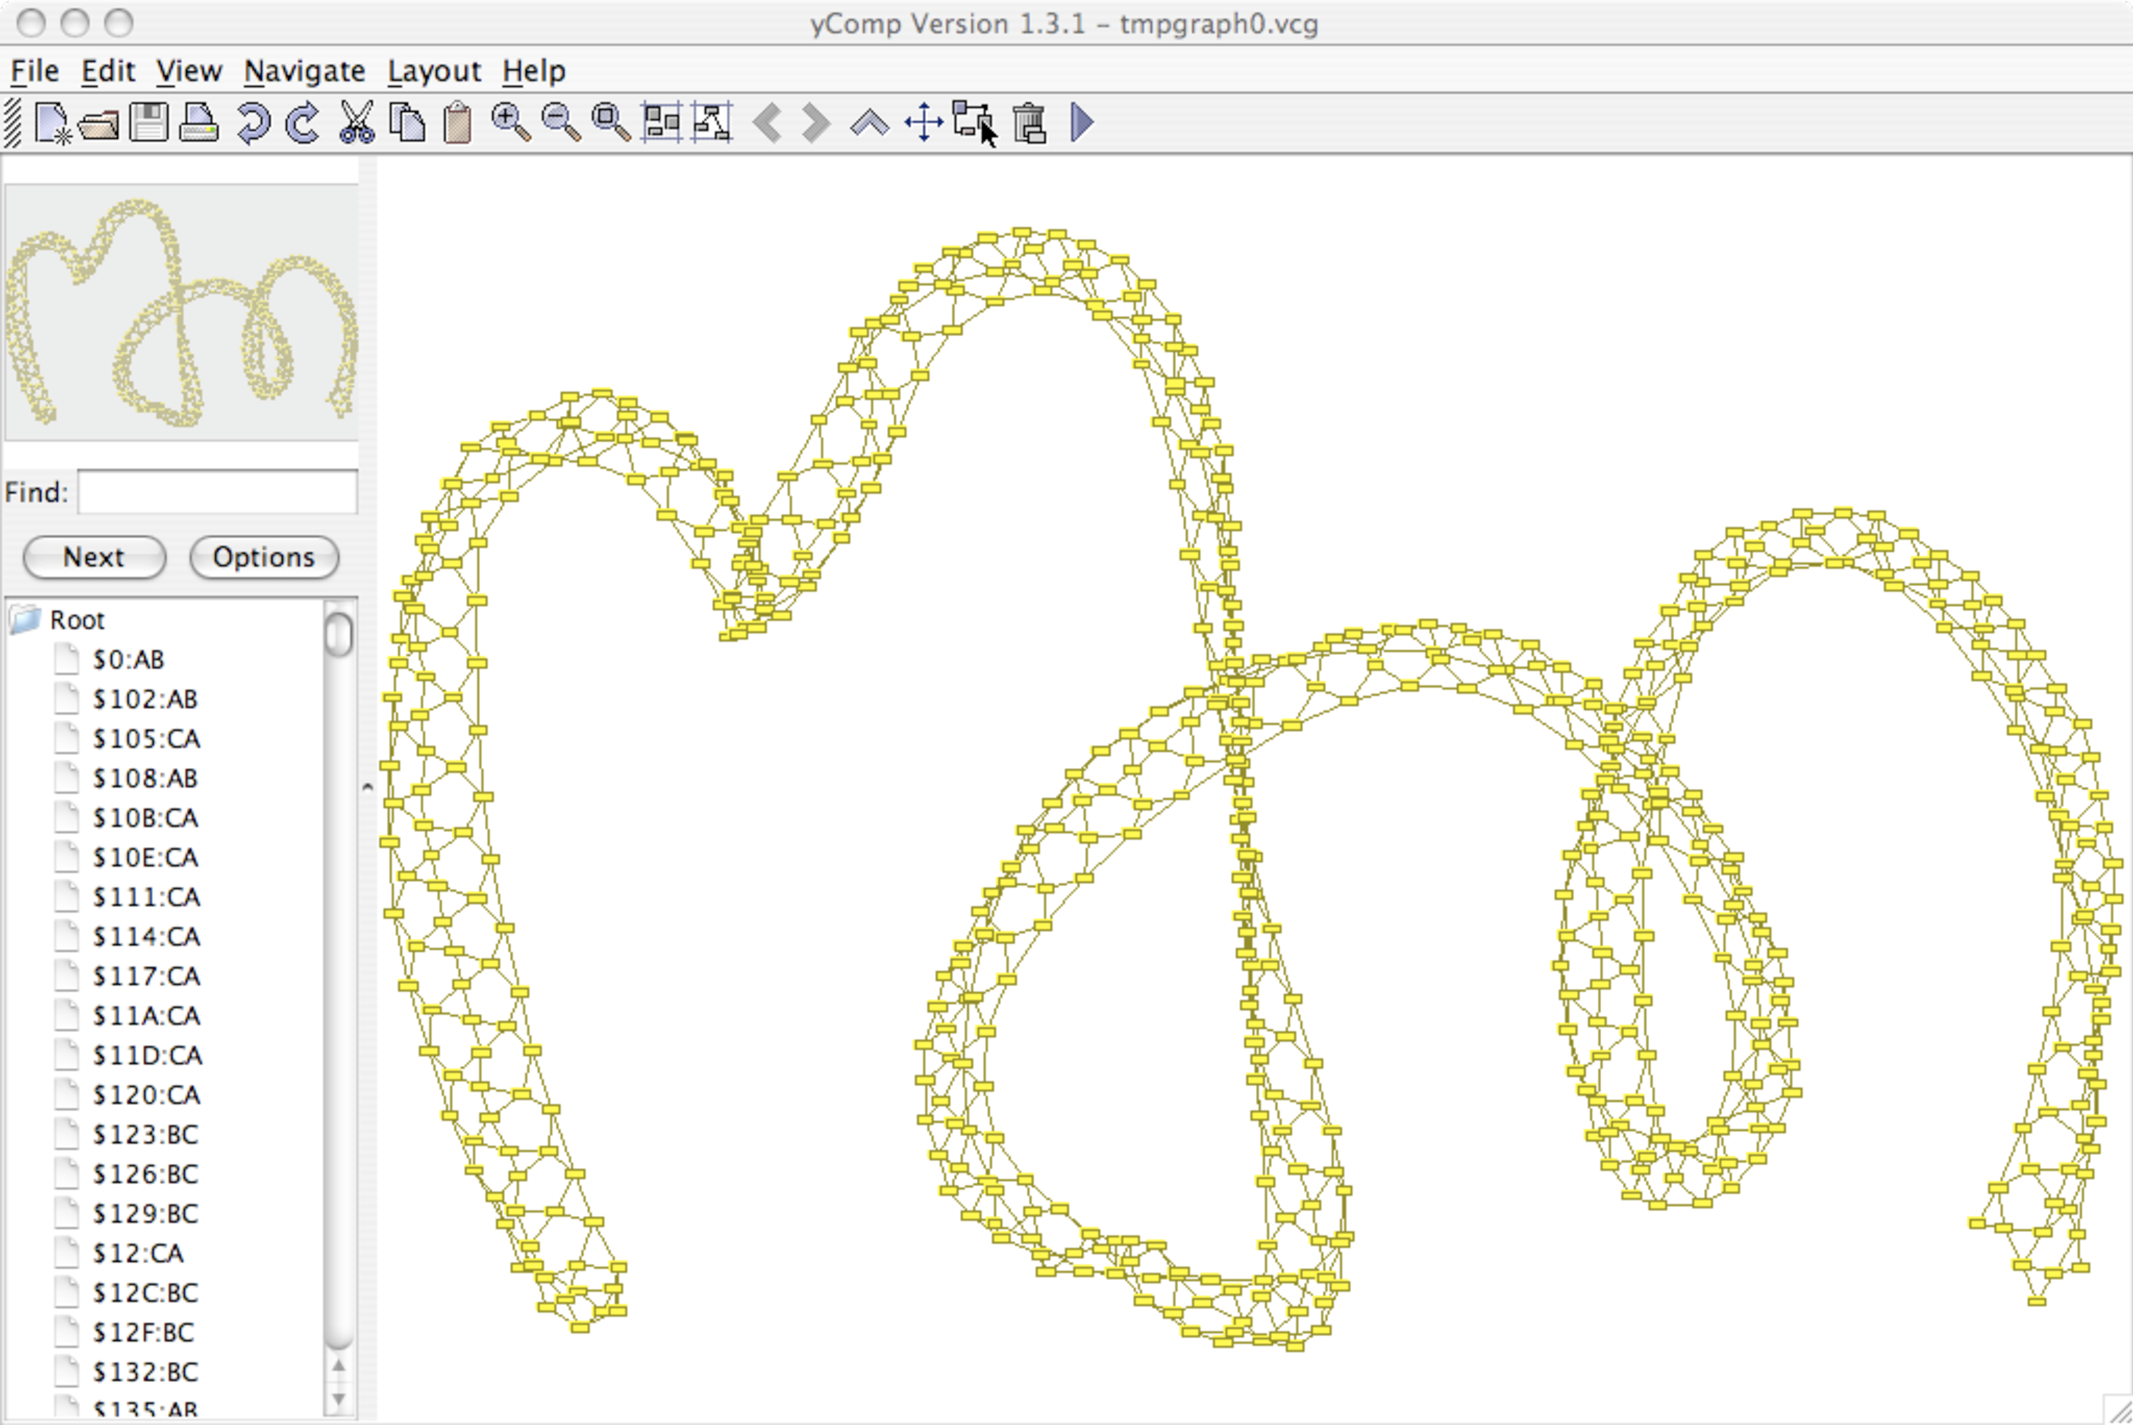
\includegraphics[width=0.75\linewidth]{fig/showgraph}
\end{center}  
The temporary file will be deleted, when the application \emph{Filename} is terminated if \GrShell\ is still running at this time.

\begin{rail}
  'dump' 'graph' Filename
\end{rail}\ixkeyw{dump}\ixkeyw{graph}
Dumps the current graph in \indexed{VCG} format into the file \emph{Filename}.\\

The following commands control the style of the VCG output. This affects \texttt{dump graph}, \texttt{show graph}, and \texttt{enable debug}. 
\begin{rail}
  'dump' 'set' 'node' (() | 'only') NodeType \\ (('color' | 'textcolor' | 'bordercolor') Color | 'shape' Text | 'labels' ('on' | 'off' | Text)) ;
\end{rail}\ixkeyw{dump}\ixkeyw{set}\ixkeyw{node}\ixkeyw{only}\ixkeyw{color}\ixkeyw{textcolor}\ixkeyw{bordercolor}\ixkeyw{shape}\ixkeyw{labels}
Sets the \indexed{color}, text color, border color, the shape or the label of the nodes of type \emph{NodeType} and all of its subtypes.
The keyword \texttt{only} excludes the subtypes. The available colors are specified at the begin of this chapter. 
The following shapes are supported: \texttt{box}, \texttt{triangle}, \texttt{circle}, \texttt{ellipse}, \texttt{rhom}, \texttt{hexagon}, \texttt{trapeze}, \texttt{uptrapeze}, \texttt{lparallelogram}, \texttt{rparallelogram}.
Those are shape names of \yComp\ (for a VCG definition see~\cite{vcg}).
The default labeling is set to \texttt{on} with \texttt{Name:Type}, it can be overwritten by an specified label string (e.g. the source code line originating the node in a program graph) or switched off.

\begin{rail}
  'dump' 'set' 'edge' (() | 'only') EdgeType \\ (('color' | 'textcolor') Color | 'labels' ('on' | 'off' | Text));
\end{rail}\ixkeyw{dump}\ixkeyw{set}\ixkeyw{edge}\ixkeyw{only}\ixkeyw{color}\ixkeyw{textcolor}\ixkeyw{labels}
Sets the color, text color or label of the edges of type \emph{EdgeType} and all of its subtypes.
The keyword \texttt{only} excludes the subtypes. The available colors are specified at the begin of this chapter.
The default labeling is set to \texttt{on} with \texttt{Name:Type}, it can be overwritten by an specified label string or switched off.

\begin{rail}
  'dump' 'add' 'node' ('only')? NodeType 'exclude' ;
\end{rail}\ixkeyw{dump}\ixkeyw{add}\ixkeyw{node}\ixkeyw{only}\ixkeyw{exclude}
Excludes nodes of type \emph{NodeType} and all of its subtypes as well as their incident edges from output.
The keyword \texttt{only} excludes the subtypes from exlusion, i.e.\ subtypes of \emph{NodeType} are dumped.

\begin{rail}
  'dump' 'add' 'node' ('only')? NodeType 'group' (GroupConstraints)? ;
GroupConstraints:
  'by' ('hidden')? GroupMode (IncAdjTypeConstraints)? ;
IncAdjTypeConstraints:
  ('only')? EdgeType ('with' ('only')? NodeType)? ;
\end{rail}\ixkeyw{dump}\ixkeyw{add}\ixkeyw{node}\ixkeyw{group}
Declares \emph{NodeType} and subtypes of \emph{NodeType} as \indexed{group node} type.
All the differently typed nodes that point to a node of type \emph{NodeType} 
(i.e.\ there is a directed edge between such nodes) will be grouped and visibly enclosed by the \emph{NodeType}-node.
\texttt{GroupMode} is one of \texttt{no},\texttt{incoming},\texttt{outgoing},\texttt{any}; \texttt{hidden} causes hiding of the edges by which grouping happens.
The \texttt{EdgeType} constrains the type of the edges which cause grouping, the \texttt{with} clause additionally constains the type of the adjacent node; 
\texttt{only} excludes subtypes.

The following example shows \emph{metropolis} ungrouped and grouped:
\begin{center}
  \fbox{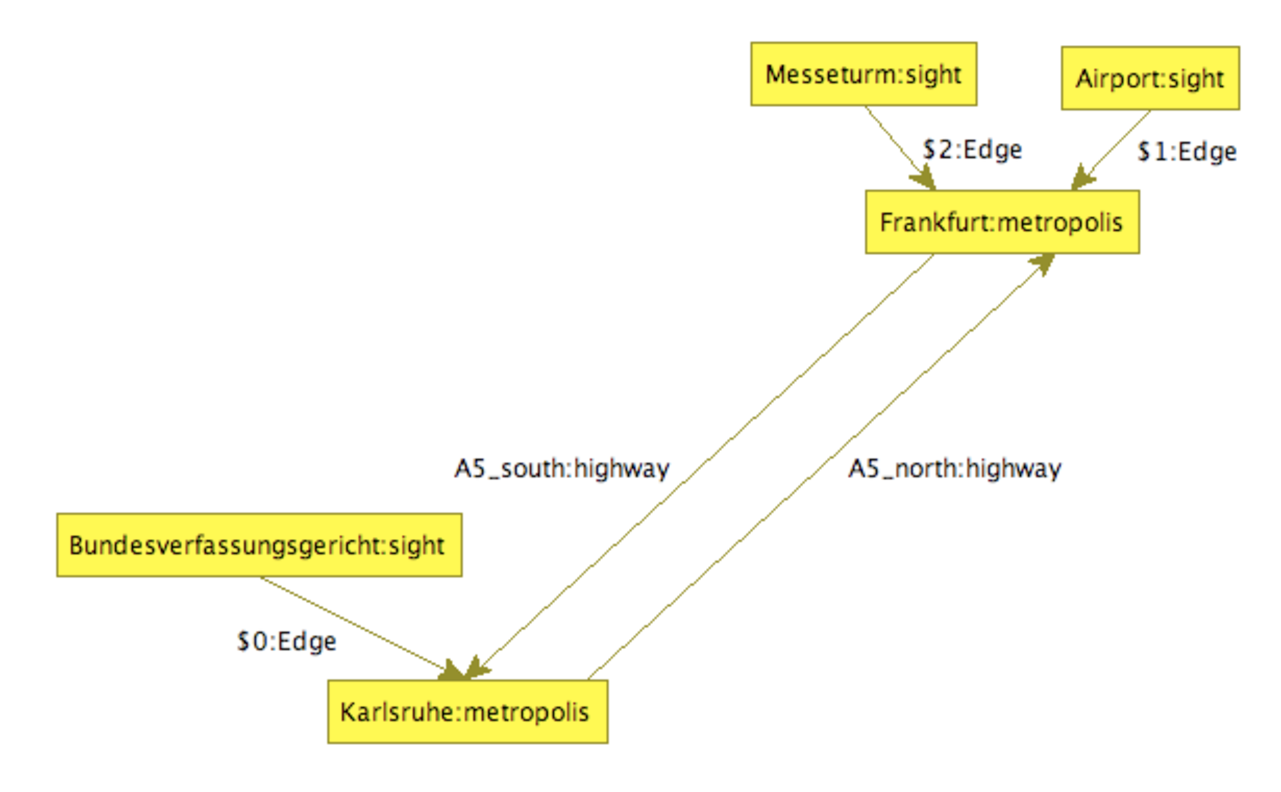
\includegraphics[width=0.45\linewidth]{fig/group2-1}}  \hfill \fbox{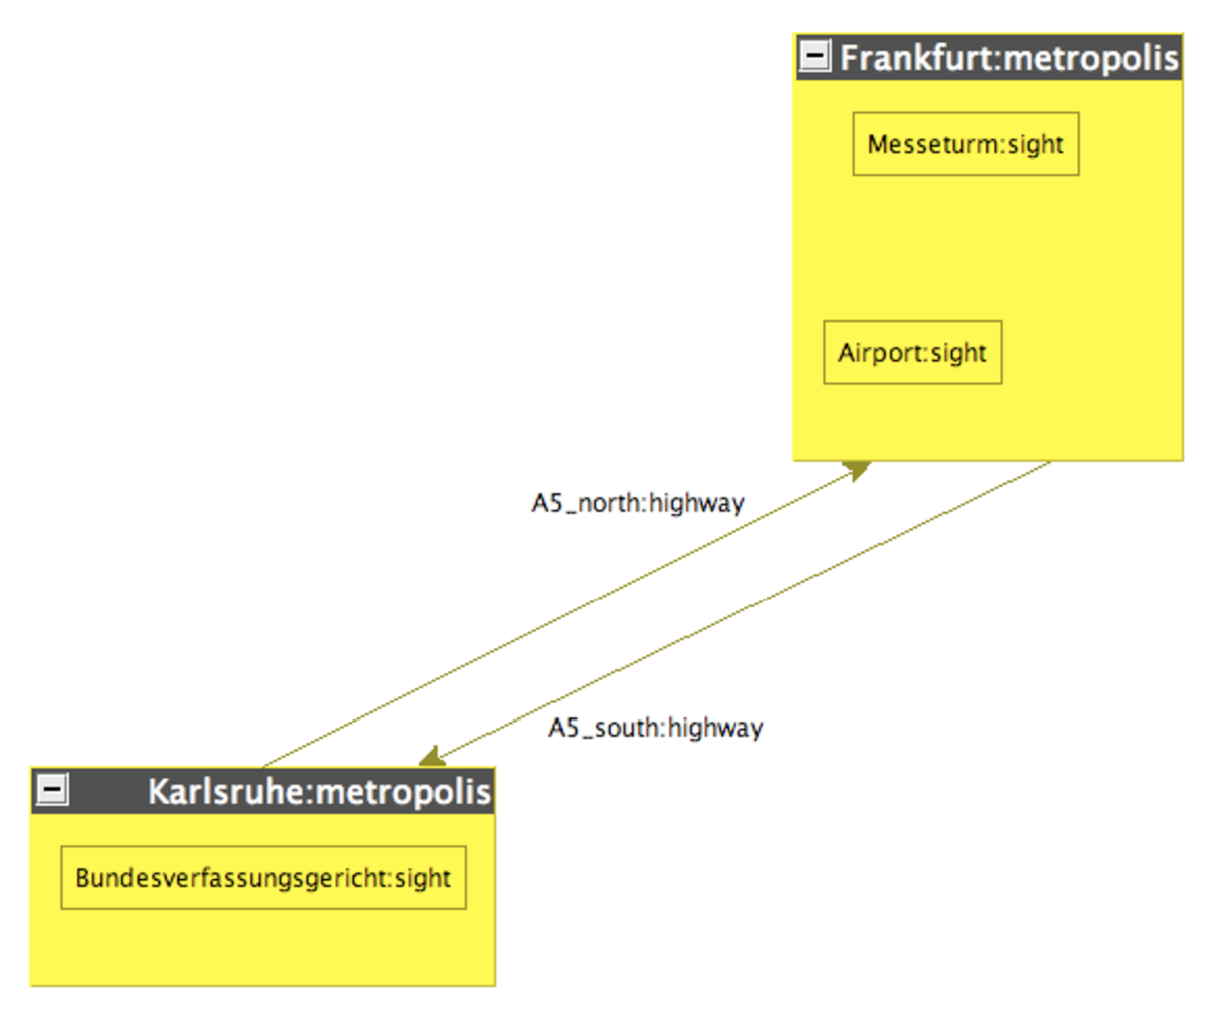
\includegraphics[width=0.45\linewidth]{fig/group2-2}}\\
  {\small right side: dumped with \texttt{dump add node metropolis group}}
\end{center}

\begin{rail}
  'dump' 'add' (() | 'only') ('node' NodeType | 'edge' EdgeType) \\ ('infotag' | 'shortinfotag') AttributeName
\end{rail}\ixkeyw{dump}\ixkeyw{add}\ixkeyw{only}\ixkeyw{node}\ixkeyw{edge}\ixkeyw{infotag}
Declares the \indexed{attribute} \emph{AttributeName} to be an ``\indexed{info tag}'' or ``\indexed{short info tag}''.
Info tags are displayed like additional node/edge \indexed{label}s, in format \texttt{Name=Value}, or \texttt{Value} only for short info tags. 
The keyword \texttt{only} excludes the subtypes of \emph{NodeType} resp.\ \emph{EdgeType}. 
In the following example \emph{river} and \emph{jam} are info tags:
\begin{center}
  \fbox{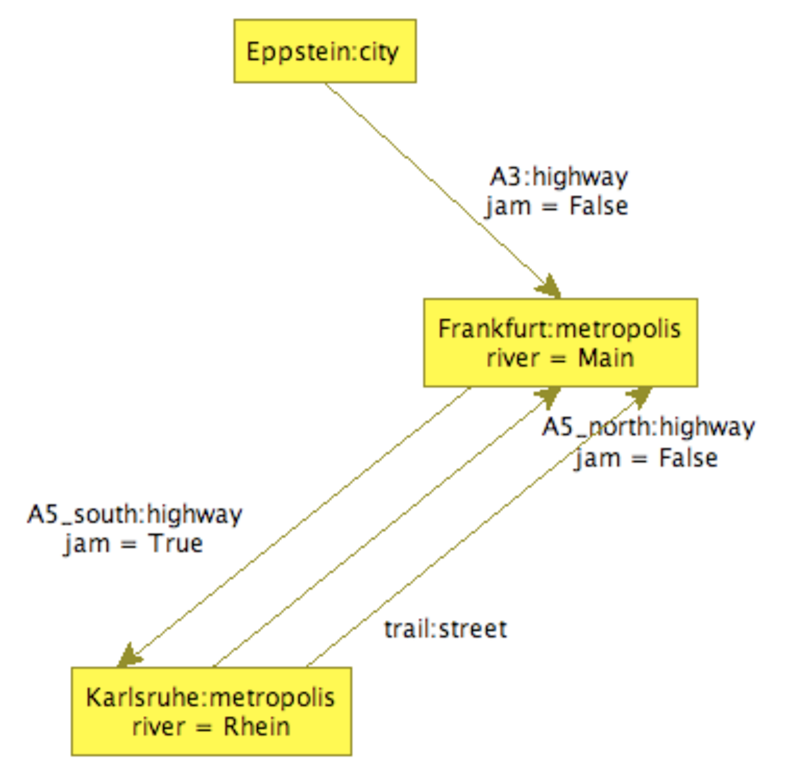
\includegraphics[width=0.5\linewidth]{fig/infotag}}
\end{center}

\begin{rail}
  'dump' 'reset'
\end{rail}\ixkeyw{dump}\ixkeyw{reset}
Resets all style options (\texttt{dump set}\dots) to their default values.


\begin{note}
Small graphs allow for fast visual understanding, but with an increasing number of nodes and edges they quickly loose this property.
The group commands are of outstanding importance to keep readability with increasing graph sizes
(e.g. for program graphs it allows to lump together expressions of a method inside the method node and attributes of the class inside the class node).
Additional helpers in keeping the graph readable are: 
the capability to exclude elements from dumping (the less hay in the stack the easier to find the needle),
the different colors and shapes to quickly find the elements of interest,
as well as the labels/infotags/shortinfotags to display the most important information directly. 
Choose the layout algorithm and the options delivering the best results for your needs, organic and compiler graph 
(an extension of hierarchic with automatic edge cutting -- marking cut edges by fat dots, showing the edge only on mouse over and allowing to jump to the other end on a mouse click)
should be tried first.
\end{note}


\subsection{Action Commands (XGRS)}\indexmain{action command}\indexmainsee{action}{graph rewrite sequence}
\label{grsthings}
An \emph{action} denotes a graph rewrite rule.

\begin{rail}
  'select' 'actions' Filename
\end{rail}\ixkeyw{select}\ixkeyw{actions}
Selects a \indexed{rule set}.
\emph{Filename} can either be a .NET assembly (e.g.\ ``rules.dll'') or a source file (``rules.cs'').
Only one rule set can be loaded simultaneously.

\begin{rail}
  'show' 'actions'
\end{rail}\ixkeyw{show}\ixkeyw{actions}
Lists all the rules of the loaded rule set, their parameters, and their return values.
Rules can return a set of graph elements.

\begin{rail}
  'custom' 'actions' (() | SpacedParameters)
\end{rail}\ixkeyw{custom}\ixkeyw{actions}
Executes an action specific to the current \indexed{backend}. 
If \emph{SpacedParameters} is omitted, a list of available commands will be displayed (for the LGSPBackend see Section~\ref{custom}).

\makeatletter
\begin{rail}
  GraphRewriteSequence: 'xgrs' SimpleRewriteSequence ;
\end{rail}\ixkeyw{grs}\indexmain{graph rewrite sequence}\indexmainsee{GRS}{graph rewrite sequence}\ixnterm{GraphRewriteSequence}
This executes the graph rewrite sequence \emph{SimpleRewriteSequence}.
See section \ref{sct:xgrs} for graph rewrite sequences.
Additionally to the variable assignment in rule-embedded graph rewrite sequences, you are also able to assign \emph{persistent names} to parameters via  \texttt{Variable = \@(Text)}.

Graph elements returned by rules can be assigned to variables\indexmain{variable} using \texttt{(Para\-meters) = \emph{Action}}\indexmain{parameter}. 
The desired variable identifiers have to be listed in \emph{Parameters}. 
Graph elements required by rules must be provided using \texttt{Action (Para\-meters)}, where \emph{Parameters} is a list of variable identifiers. 
For \indexed{undefined variables} see Section~\ref{ruledecls}, \emph{Parameters}.

% don't explain set/map commands, as they will be replaced by graph rewrite sequence terms
% they are given in the changelog, so if someone needs them now they are there
% but not fully officially documented, so that they can be dropped as soon as the sequences are extended


\section{Graphical Debugger}
\label{sct:debugger}
The \GrShell\ together with \yComp\ build \GrG's graphical debugger.

\subsection{Debugging Related Commands}

\begin{rail}
  'debug' ( 'enable' | 'disable' )
\end{rail}\ixkeyw{debug}\ixkeyw{enable}\ixkeyw{disable}
Enables and disables the \indexed{debug mode}.
The debug mode shows the current working graph in a \yComp\ window.
All changes to the working graph are tracked by \yComp\ immediately.  

\begin{rail}
  'debug' 'set' 'layout' ( (Text)? | 'option' Name String ) ;
\end{rail}\ixkeyw{debug}\ixkeyw{set}\ixkeyw{layout}
Sets the default graph \indexed{layout algorithm} to \emph{Text}.
If \emph{Text} is omitted, a list of available layout algorithms is displayed.
See Section~\ref{tools:ycomp} on \yComp\ layouters.
The \texttt{option} version allows to specify layout options by name value pairs.
The available layout options can be listed by the following command.

\begin{rail}
  'debug' 'get' 'layout' 'options';
\end{rail}\ixkeyw{debug}\ixkeyw{layout}
Prints a list of the available layout options of the layout algorithm.

\begin{rail}
  'debug' 'layout';
\end{rail}\ixkeyw{debug}\ixkeyw{layout}
Forces re-layout of the graph shown in yComp (same as pressing the play button within yComp).

\begin{rail}
  GraphRewriteSequence: 'debug' 'xgrs' SimpleRewriteSequence ;
\end{rail}\ixkeyw{debug}\ixkeyw{grs}\indexmain{graph rewrite sequence}\indexmainsee{GRS}{graph rewrite sequence}\ixnterm{GraphRewriteSequence}
This executes the graph rewrite sequence \emph{SimpleRewriteSequence} in the debugger\indexmain{debugger}.
Same as \texttt{xgrs SimpleRewriteSequence} in the previous section, but allows tracing the rewriting process step-by-step. 

\begin{rail}
'debug' 'apply' Rule
\end{rail}\ixkeyw{debug}\ixkeyw{apply}
The \texttt{debug apply} command allows to interactively select parameters for the execution of the rule \texttt{Rule}.
The parameters to select are specified by the wildcard elements \texttt{?}, they are given by double clicking at elements in the graph viewer yComp.

\begin{example}
\begin{grshelllet}
debug apply r(?, x, ?)
\end{grshelllet}
will prompt the user for input of the first and the third parameter, while the second one is taken from variable x.
\end{example}


\subsection{Using the Debugger}

During execution \yComp\footnote{Make sure, that the path to your \texttt{\indexed{yComp.jar}} package is set correctly in the \texttt{ycomp} shell script within \GrG's \texttt{/bin} directory.}
\indexmain{yComp} will display every single step. 
The debugger\indexmain{debugger} can be controlled by \GrShell. 
Remember that the \texttt{\%} modifier before a rule works as break point in a graph rewrite sequence.
The debug commands are shown in Table~\ref{tabdebug}. A run is shown in the following example \ref{ex:debug}.
\begin{table}[htbp]
  \begin{tabularx}{\linewidth}{|lX|} \hline
  \texttt{s}(tep) & Execute the next rewrite rule (match and rewrite)\\
  \texttt{d}(etailed step) & Execute a rewrite rule in a three-step procedure: matching, highlighting elements to be changed, doing rewriting \\
  \texttt{n}(ext) & Ascend one level up within the \indexed{Kantorowitsch tree} of the current rewrite sequence (see Example~\ref{ex:debug})\\
  (step) \texttt{o}(ut) & Continue execution until the end of the current loop. If the execution is not in a loop at this moment, the complete sequence will be executed\\
  (toggle) \texttt{b}(reakpoint) & Toggle a breakpoint at a rewrite rule, a true, or a false\\
  \texttt{r}(un) & Continue execution\\
  \texttt{a}(bort) & Cancel the execution immediately\\ \hline 
  \end{tabularx}
  \caption{\GrShell\ debug commands}
  \label{tabdebug}
\end{table}
%\begin{figure}[htbp]
%  \centering
%  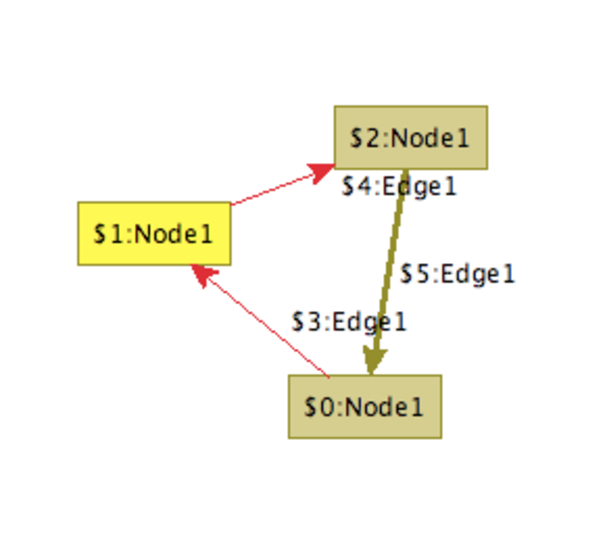
\includegraphics[width=0.25\linewidth]{fig/debug1}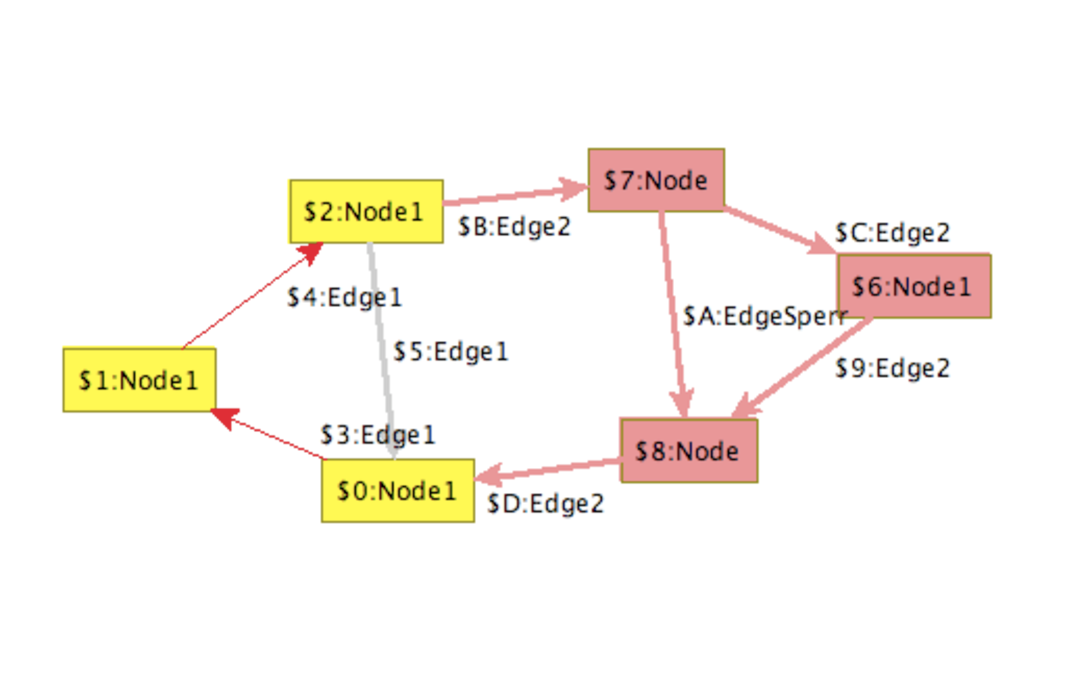
\includegraphics[width=0.4\linewidth]{fig/debug2}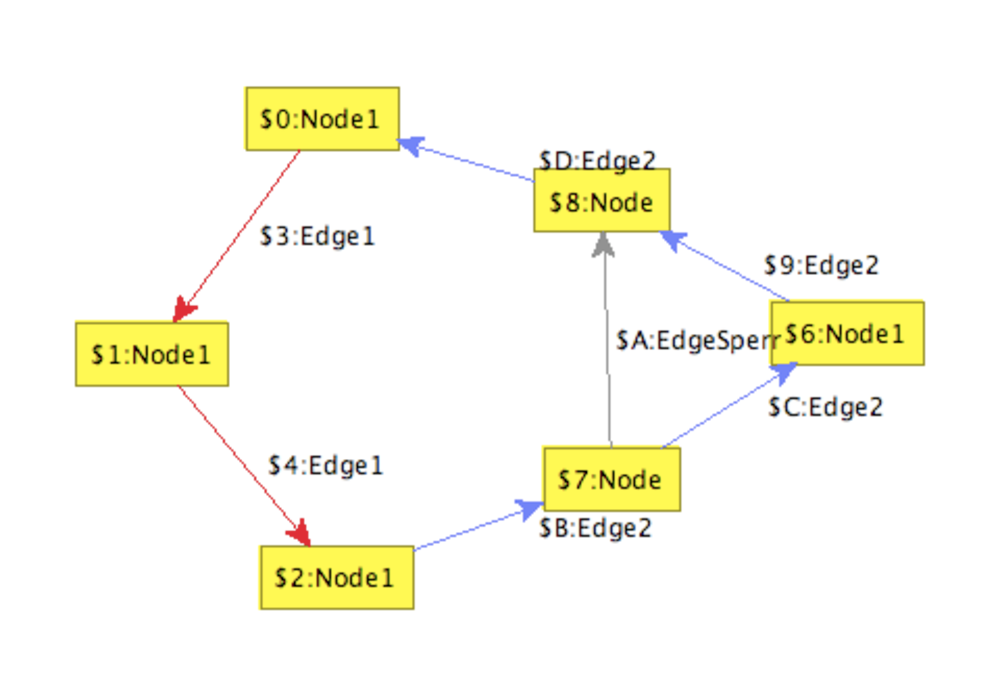
\includegraphics[width=0.4\linewidth]{fig/debug3}
%  \caption{Delayed step rule application.}
%  \label{figdebug}
%\end{figure}

\begin{figure}[htbp]
\begin{example}\label{ex:debug}  
We demonstrate the debug commands with a slightly adjusted script for the Koch snowflake from \GrG's examples (see also Section~\ref{fractals}). The graph rewriting sequence is
\begin{grshell}
debug xgrs (makeFlake1* & (beautify & doNothing)* & makeFlake2* & beautify*)[1]
\end{grshell}
\yComp\ will be opened with an initial graph (resulting from \texttt{grs init}):
\begin{center}
  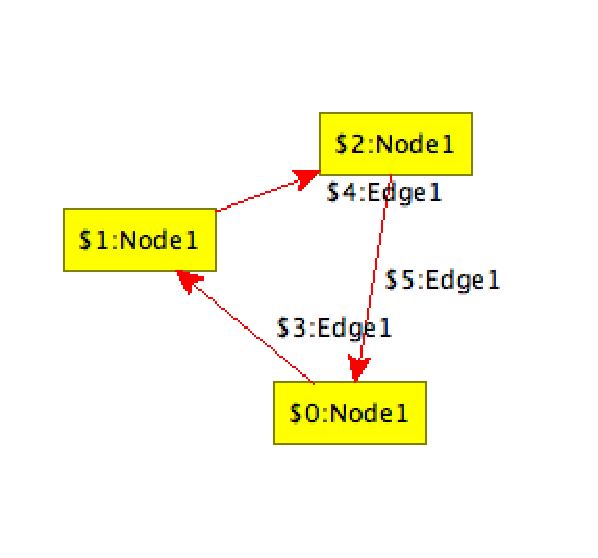
\includegraphics[width=0.3\linewidth]{fig/debug0tra}
\end{center}
We type \texttt{d}(etailed step) to apply \texttt{makeFlake1} step by step resulting in the following graphs:
\begin{center}
  \parbox{0.2\linewidth}{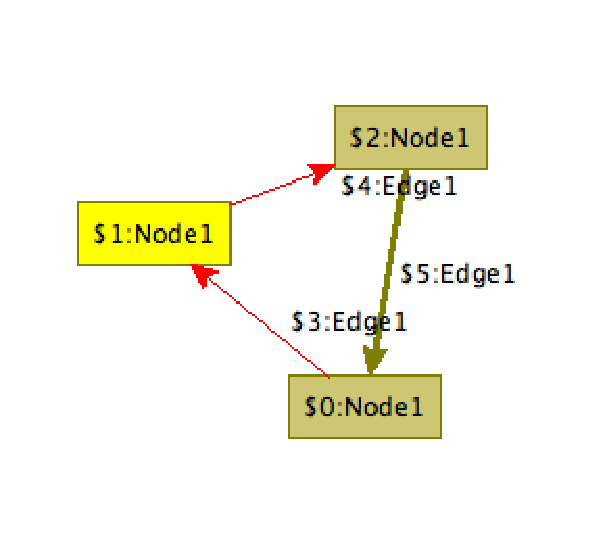
\includegraphics[width=\linewidth]{fig/debug1tra}}\parbox{0.375\linewidth}{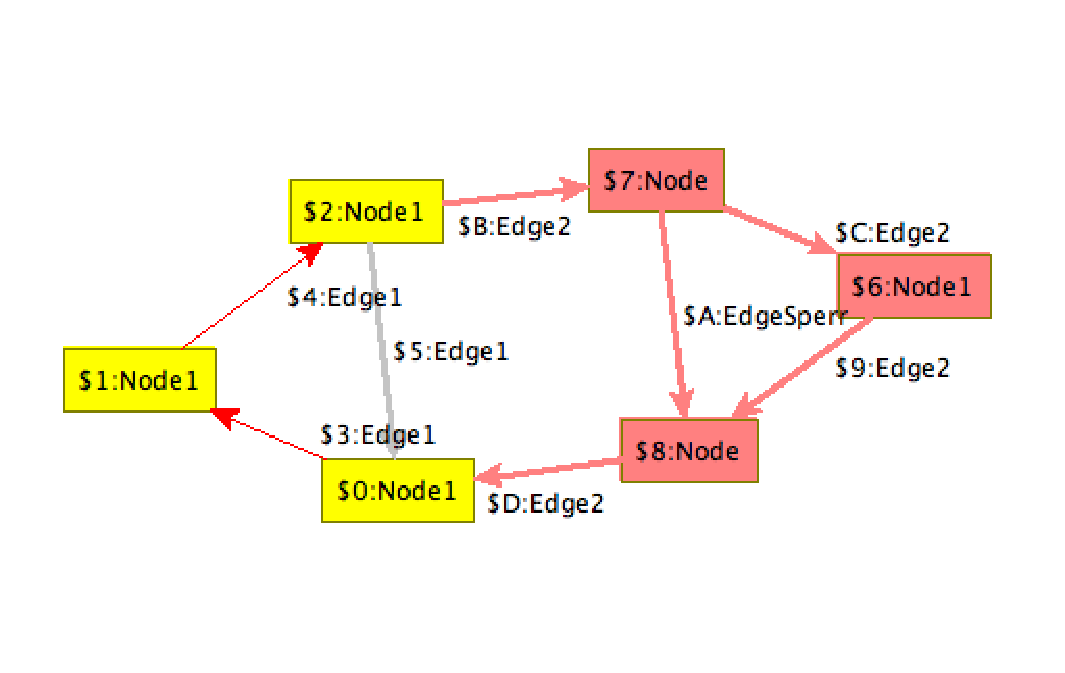
\includegraphics[width=\linewidth]{fig/debug2tra}}\parbox{0.375\linewidth}{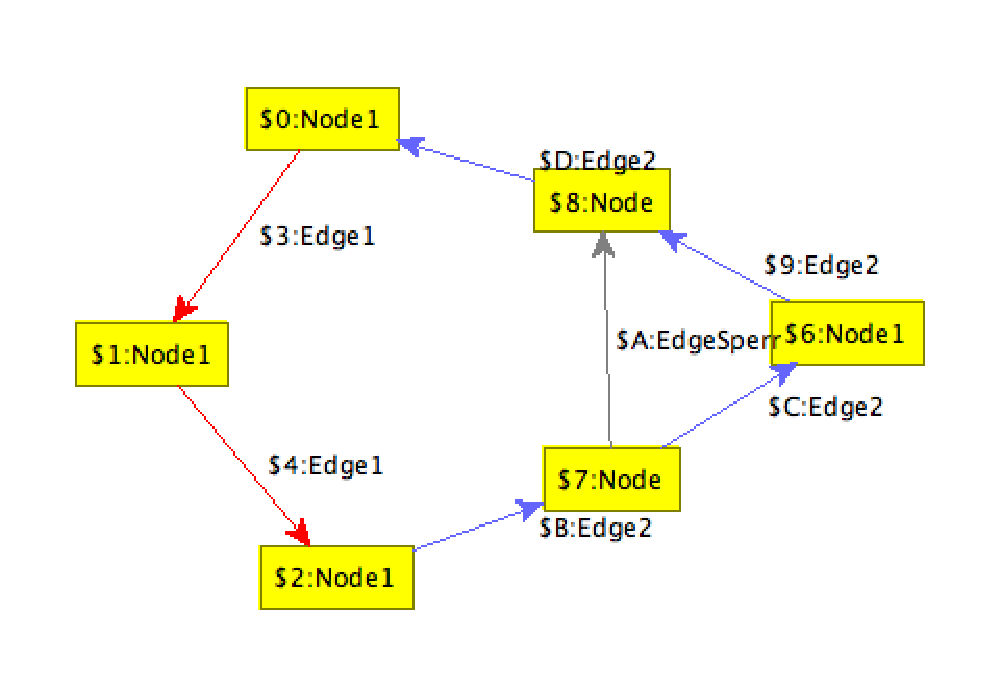
\includegraphics[width=\linewidth]{fig/debug3tra}}
\end{center}
The following table shows the ``break points'' of further debug commands, entered one after another:
\begin{center}
  \begin{tabular}{|l|l|} \hline
    \textbf{Command} & \textbf{Active rule} \\ \hline
    \texttt{s} & \texttt{makeFlake1} \\
    \texttt{o} & \texttt{beautify} \\
    \texttt{s} & \texttt{doNothing} \\
    \texttt{s} & \texttt{beautify} \\ 
    \texttt{n} & \texttt{beautify} \\ 
    \texttt{o} & \texttt{makeFlake2} \\
    \texttt{r} & --- \\ \hline
  \end{tabular}
\end{center}
\end{example}   
\end{figure}


\section{Backend Commands}
\label{backend}

\GrG\ is built to support multiple backends implementing the model and action interfaces of libGr.
This is roughly comparable to the different storage engines MySQL offers.
Currently only one backend is available, the libGr search plan backend, or short LGSPBackend.

\subsection{Backend selection and custom commands}

\begin{rail}
  'select' 'backend' Filename ( ( ) | ':' Parameters )
\end{rail}\ixkeyw{select}\ixkeyw{backend}
Selects a \indexed{backend} that handles graph and rule representation.
\emph{Filename} has to be a .NET assembly (e.g.\ \texttt{lgspBackend.dll}\indexmain{LGSPBackend}).
Comma-separated \indexed{parameter}s can be supplied optionally; if so, the backend must support these parameters.
By default the LGSPBackend is used.

\begin{rail}
  'show' 'backend'
\end{rail}\nopagebreak\ixkeyw{show}\ixkeyw{backend}
List all the parameters supported by the currently selected backend.
The parameters can be provided to the \texttt{select backend} command.

\begin{rail}
  'custom' 'graph' ( ( ) | SpacedParameters )
\end{rail}\ixkeyw{custom}\ixkeyw{graph}
Executes a command specific to the current backend.
If \emph{SpacedParameters} is omitted, a list of available commands will be displayed (for the LGSP backend see Sections~\ref{custom}).


\subsection{LGSPBackend Custom Commands}
\label{custom}

The \indexed{LGSPBackend} supports the following custom commands:

\begin{rail}
  'custom' 'graph' analyzegraph
\end{rail}\ixkeyw{custom}\ixkeyw{graph}
Analyzes\indexmain{analyzing graph} the current working graph.
The analysis data provides vital information for efficient \indexed{search plan}s.
Analysis data is available as long as \GrShell\ is running, i.e.\ when the working graph changes, the analysis data is still available but maybe obsolete.

\begin{rail}
  'custom' 'actions' gensearchplan (Action+)
\end{rail}\ixkeyw{custom}\ixkeyw{actions}
Creates a search plan for each rewrite rule \emph{Action} using a heuristic method and the analyzes data (if the graph has been analyzed by \texttt{custom graph analyze\_graph}).
Otherwise a \indexed{default search plan} is used.
For efficiency reasons it is recommended to do analyzing and search plan creation during the rewriting procedure.
Therefore the host graph should be in a stage ``similar'' to the final result.
Indeed there might be some trial-and-error steps necessary to get an efficient search plan.
A search plan is available as long as the current rule set remains loaded. 
Specify multiple rewrite rules instead of using multiple commands for each rule to improve the search plan generation performance.

\begin{rail}
  'custom' 'actions' setmaxmatches Number
\end{rail}\ixkeyw{custom}\ixkeyw{actions}
Sets the maximum amount of possible pattern matches to \emph{Number}.
This command affects the expression \texttt{[\emph{Rule}]}.
If \emph{Number} is less or equal to zero, the constraint is reset.



\chapter{Visualization and Debugging}\indexmain{Debugger}
\label{chapdebugger}

This chapter gives an introduction into the visualization capabilities of yComp and into the graphical debugger of \GrG, which is offered by \GrShell\ in combination with yComp.

Other commands of use for debugging were already introduced in the shell chapter:
\verb#show var <Variable># to print the content of a variable (but pressing the \texttt{v} key in the shell debugger is a lot more convenient) and \verb#show <GraphElement>.<AttributeName># to print the content of an attribute (but searching with \texttt{Ctrl-f} or \texttt{/} in yComp for the persistent name or an attribute value, hovering over the then highlighted graph element is more convenient, again); furthermore \verb#record# and \verb#replay# are interesting when you are debugging a transformation where you are choosing from the available matches by hand and want to try other paths later by choosing differently on a previous match: they allow you to save and restore graph states of interest, and to inspect the sequence of changes which lead to them in the \texttt{.grs}.


%%%%%%%%%%%%%%%%%%%%%%%%%%%%%%%%%%%%%%%%%%%%%%%%%%%%%%%%%%%%%%%%%%%%%%%%%%%%%%%%%%%%%%%%%%%%%%%%
\section{Graph Visualization Commands (Nested Layout)}\label{sub:visual}\indexmain{visualization}\indexmainsee{layout}{visualization}\indexmainsee{visualization}{group node}\indexmain{nested layout}\indexmainsee{nested layout}{group node}\indexmain{nested graph}\indexmainsee{nested graph}{group node}

\begin{rail}
  'show' 'graph' ExecutableName (() | Text)
\end{rail}\ixkeyw{show}\ixkeyw{graph}
Dumps the current graph in \indexed{VCG} format into a temporary file.
The temporary VCG file will be passed to the program \emph{ExecutableName} as first parameter;
further parameters, such as program options, can be specified by \emph{Text}.
If you use \yComp\footnote{See Section~\ref{tools:ycomp}.}\indexmain{yComp} as executable (\texttt{show graph ycomp}), this may look like
\begin{center}
  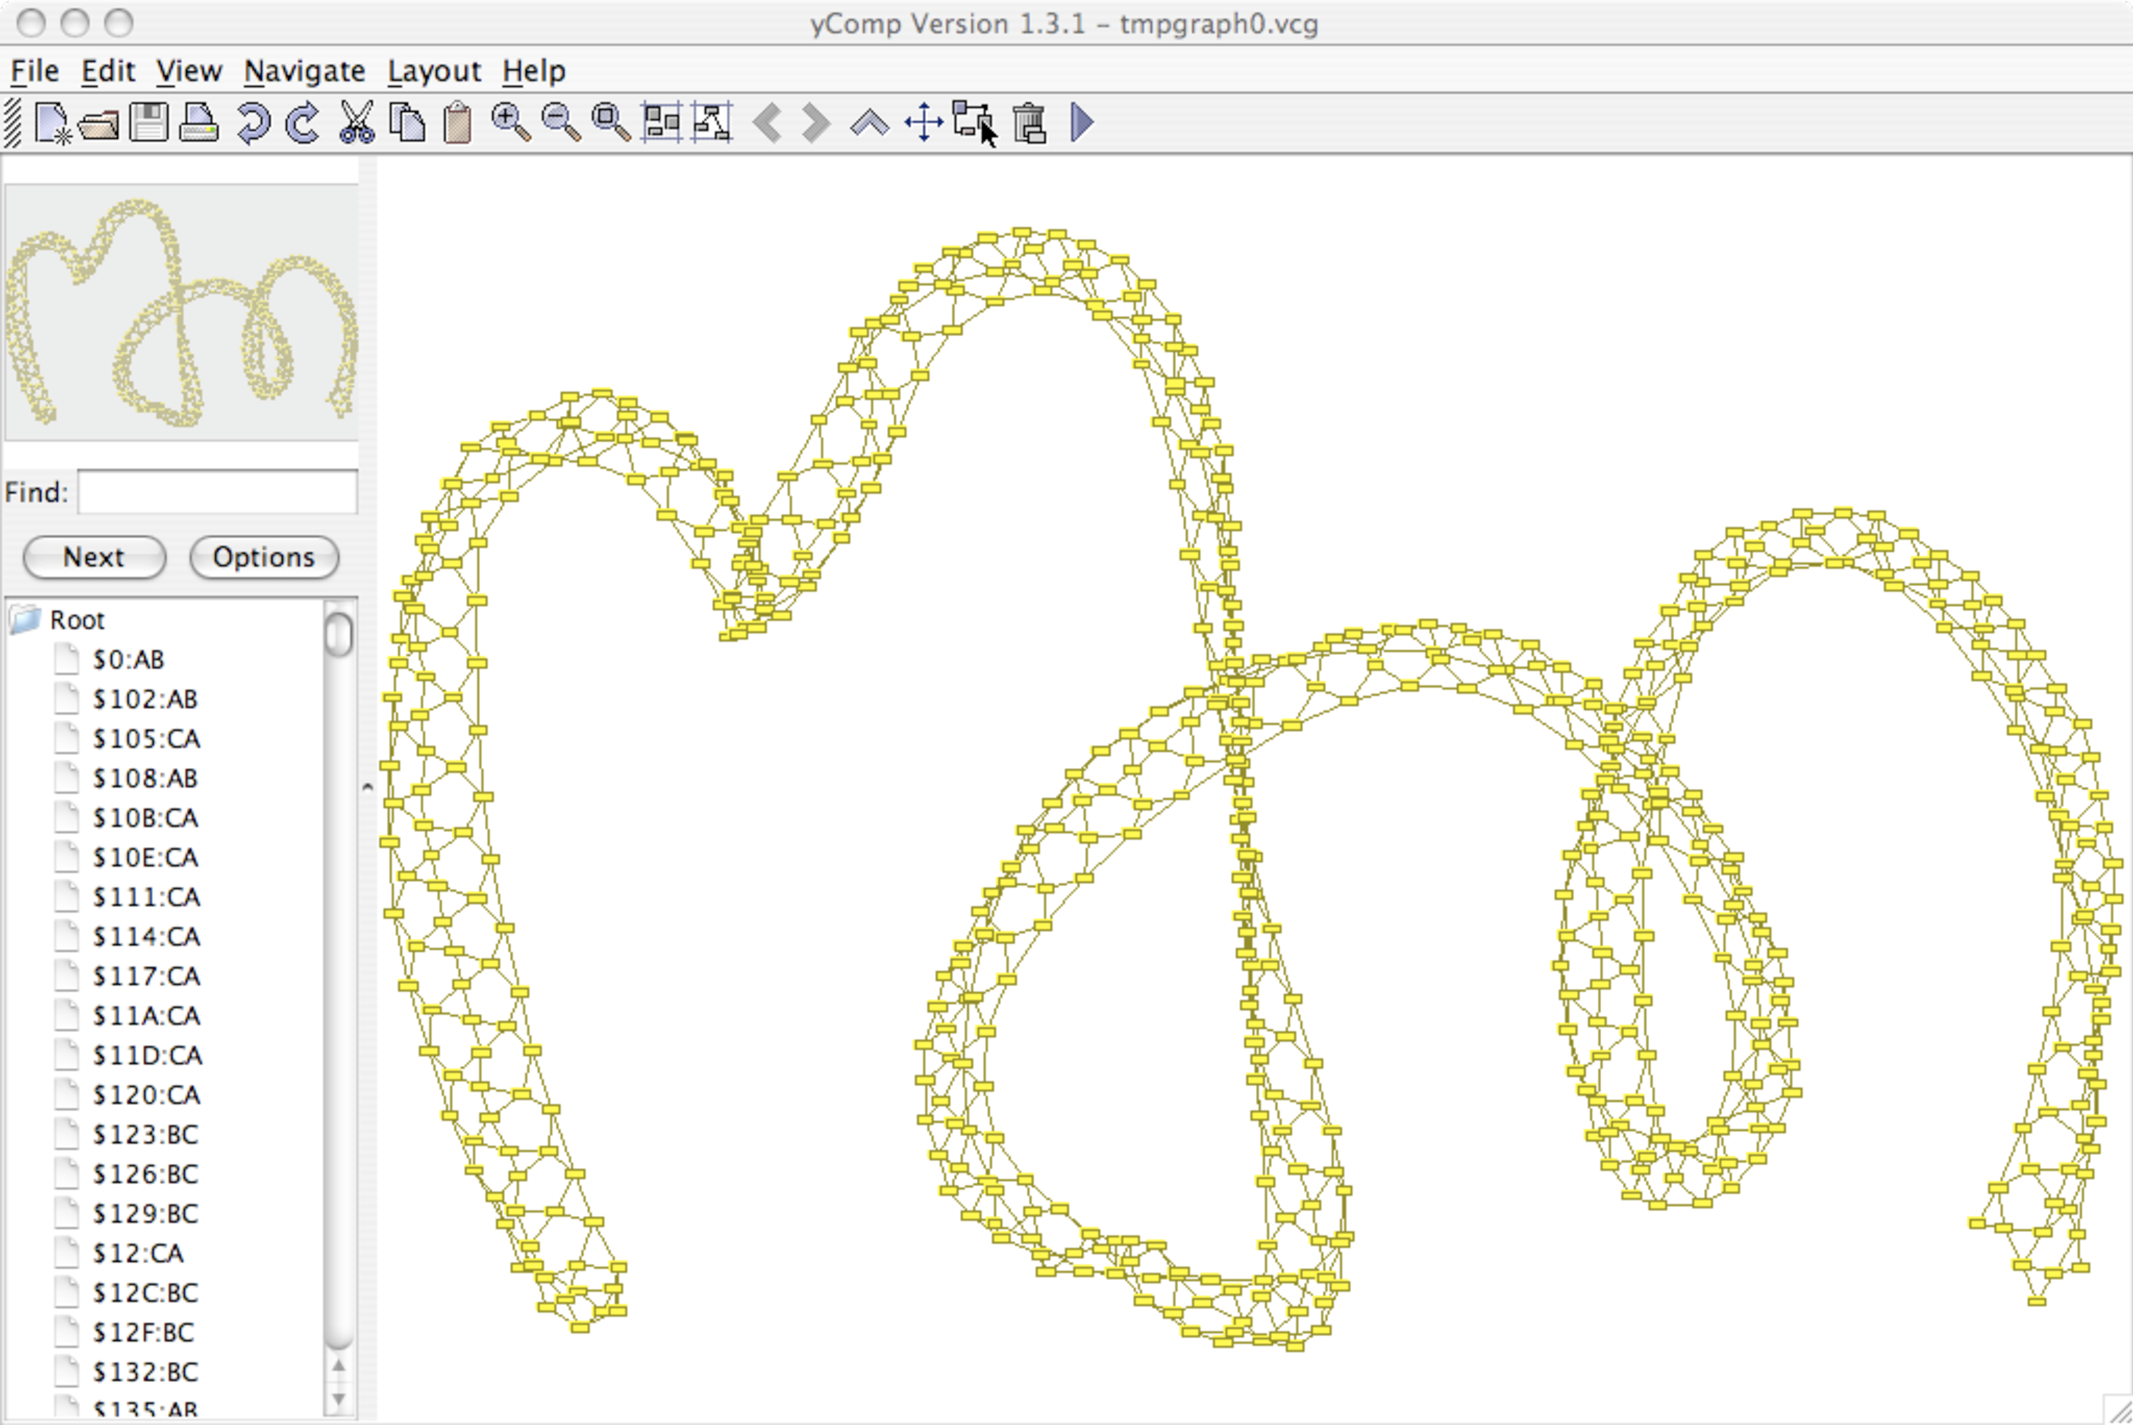
\includegraphics[width=0.75\linewidth]{fig/showgraph}
\end{center}
The temporary file will be deleted, when the application \emph{Filename} is terminated if \GrShell\ is still running at this time.

\begin{rail}
  'dump' 'graph' Filename
\end{rail}\ixkeyw{dump}\ixkeyw{graph}
Dumps the current graph in \indexed{VCG} format into the file \emph{Filename}.\\

The following commands control the style of the VCG output. This affects \texttt{dump graph}, \texttt{show graph}, and \texttt{enable debug}.
\begin{rail}
  'dump' 'set' 'node' (() | 'only') NodeType DumpNodeContinuation;
DumpNodeContinuation:
 (('color' | 'textcolor' | 'bordercolor') Color | 'shape' Text | 'labels' ('on' | 'off' | Text)) ;
\end{rail}\ixkeyw{dump}\ixkeyw{set}\ixkeyw{node}\ixkeyw{only}\ixkeyw{color}\ixkeyw{textcolor}\ixkeyw{bordercolor}\ixkeyw{shape}\ixkeyw{labels}\ixkeyw{on}\ixkeyw{off}\ixnterm{DumpNodeContinuation}
Sets the \indexed{color}, text color, border color, the shape or the label of the nodes of type \emph{NodeType} and all of its subtypes.
The keyword \texttt{only} excludes the subtypes. 
The following shapes are supported: \texttt{box}, \texttt{triangle}, \texttt{circle}, \texttt{ellipse}, \texttt{rhomb}, \texttt{hexagon}, \texttt{trapeze}, \texttt{uptrapeze}, \texttt{lparallelogram}, \texttt{rparallelogram}.
Those are shape names of \yComp\ (for a VCG definition see~\cite{vcg}).
The following colors are supported: \texttt{Black}, \texttt{Blue}, \texttt{Green}, \texttt{Cyan}, \texttt{Red}, \texttt{Purple}, \texttt{Brown}, \texttt{Grey}, \texttt{LightGrey}, \texttt{LightBlue}, \texttt{LightGreen}, \texttt{LightCyan}, \texttt{LightRed}, \texttt{LightPurple}, \texttt{Yel\-low} (default), \texttt{White}, \texttt{DarkBlue}, \texttt{DarkRed}, \texttt{Dark\-Green}, \texttt{DarkYellow}, \texttt{DarkMagenta}, \texttt{DarkCyan}, \texttt{Gold}, \texttt{Lilac}, \texttt{Turquoise}, \texttt{Aquamarine}, \texttt{Khaki}, \texttt{Pink}, \texttt{Orange}, \texttt{Orchid}, \texttt{LightYellow}, \texttt{YellowGreen}.
These are the same color identifiers as in \indexed{VCG}/\yComp\ files (for a VCG definition see~\cite{vcg}).

The default labeling is set to \texttt{on} with \texttt{Name:Type}, it can be overwritten by an specified label string (e.g. the source code line originating the node in a program graph) or switched off.

\begin{rail}
  'dump' 'set' 'edge' (() | 'only') EdgeType DumpEdgeContinuation;
DumpEdgeContinuation:
  (('color' | 'textcolor') Color | 'linestyle' (Text) | 'thickness' (Number) | 'labels' ('on' | 'off' | Text));
\end{rail}\ixkeyw{dump}\ixkeyw{set}\ixkeyw{edge}\ixkeyw{only}\ixkeyw{color}\ixkeyw{textcolor}\ixkeyw{labels}\ixkeyw{on}\ixkeyw{off}\ixkeyw{linestyle}\ixkeyw{thickness}\ixnterm{DumpEdgeContinuation}
Sets the color, text color, the linestyle, the thickness of the line, or the label of the edges of type \emph{EdgeType} and all of its subtypes.
The keyword \texttt{only} excludes the subtypes. The available colors are specified above.
The default labeling is set to \texttt{on} with \texttt{Name:Type}, it can be overwritten by an specified label string or switched off.
The following linestyles are supported: \texttt{continuous} (default), \texttt{dotted}, \texttt{dashed}.
The following thicknesses are supported: \texttt{1} (default), \texttt{2}, \texttt{3}, \texttt{4}, \texttt{5}.

\begin{rail}
  'dump' 'add' (('node' ('only')? NodeType)|('edge' ('only')? EdgeType)) 'exclude' ;
\end{rail}\ixkeyw{dump}\ixkeyw{add}\ixkeyw{node}\ixkeyw{edge}\ixkeyw{only}\ixkeyw{exclude}
Excludes nodes/edges of type \emph{NodeType}/\emph{EdgeType} and all of its subtypes from output, for a node it also excludes its incident edges.
The keyword \texttt{only} excludes the subtypes from exlusion, i.e.\ subtypes of \emph{NodeType}/\emph{EdgeType} are dumped.

\begin{rail}
  'dump' 'add' 'node' ('only')? NodeType 'group' (GroupConstraints)? ;
GroupConstraints:
  'by' ('hidden')? GroupMode (IncAdjTypeConstraints)? ;
IncAdjTypeConstraints:
  ('only')? EdgeType ('with' ('only')? NodeType)? ;
\end{rail}\ixkeyw{dump}\ixkeyw{add}\ixkeyw{node}\ixkeyw{only}\ixkeyw{group}\ixkeyw{by}\ixkeyw{hidden}\ixkeyw{with}\ixnterm{GroupConstraints}\ixnterm{IncAdjTypeConstraints}
Declares \emph{NodeType} and subtypes of \emph{NodeType} as \indexed{group node}\indexmainsee{hierarchic}{group node} type.
All the differently typed nodes that point to a node of type \emph{NodeType}
(i.e.\ there is a directed edge between such nodes) will be grouped and visibly enclosed by the \emph{NodeType}-node (nested graph).
\texttt{GroupMode} is one of \texttt{no},\texttt{incoming},\texttt{outgoing},\texttt{any}; \texttt{hidden} causes hiding of the edges by which grouping happens.
The \texttt{EdgeType} constrains the type of the edges which cause grouping, the \texttt{with} clause additionally constrains the type of the adjacent node;
\texttt{only} excludes subtypes.

\begin{warning}
Only apply group commands on a graph if they indeed lead to a containment tree of groups.
If the group commands would lead to a directed acyclic or even cyclic containment graph, the results are undefined.
You may get duplicate edges (and nodes); the implementation is free to choose indeterministically between the possible nestings -- it may even grow an arm and stab you in your back.
(A conflict resolution heuristic used is to give the earlier executed \texttt{add group} command priority.
But this mechanism is incomplete -- you'd better refine your groups or change the model in that case.
Using a model separating edges denoting direct containment from cross-linking edges by type is normally the better design, even disregarding visual node nesting.)
\end{warning}

The following example shows \emph{metropolis} ungrouped and grouped:
\begin{center}
  \fbox{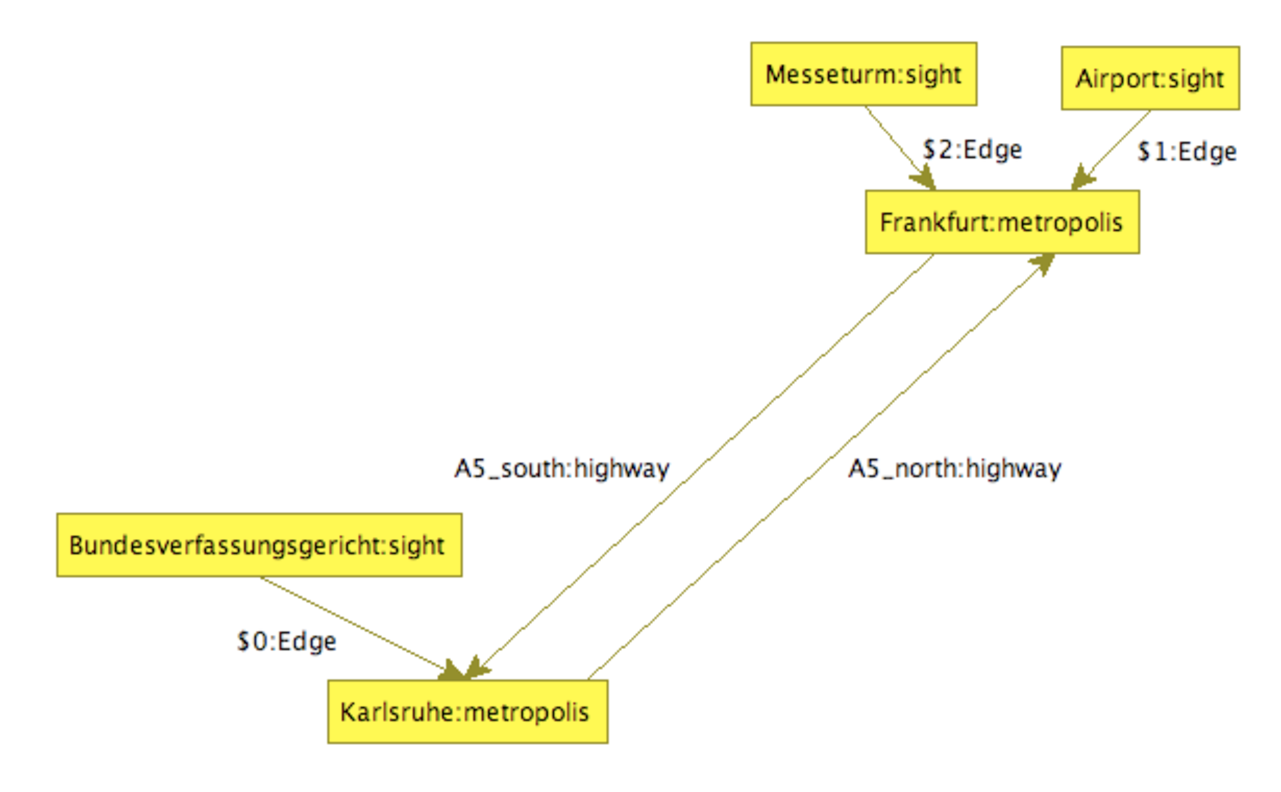
\includegraphics[width=0.45\linewidth]{fig/group2-1}}  \hfill \fbox{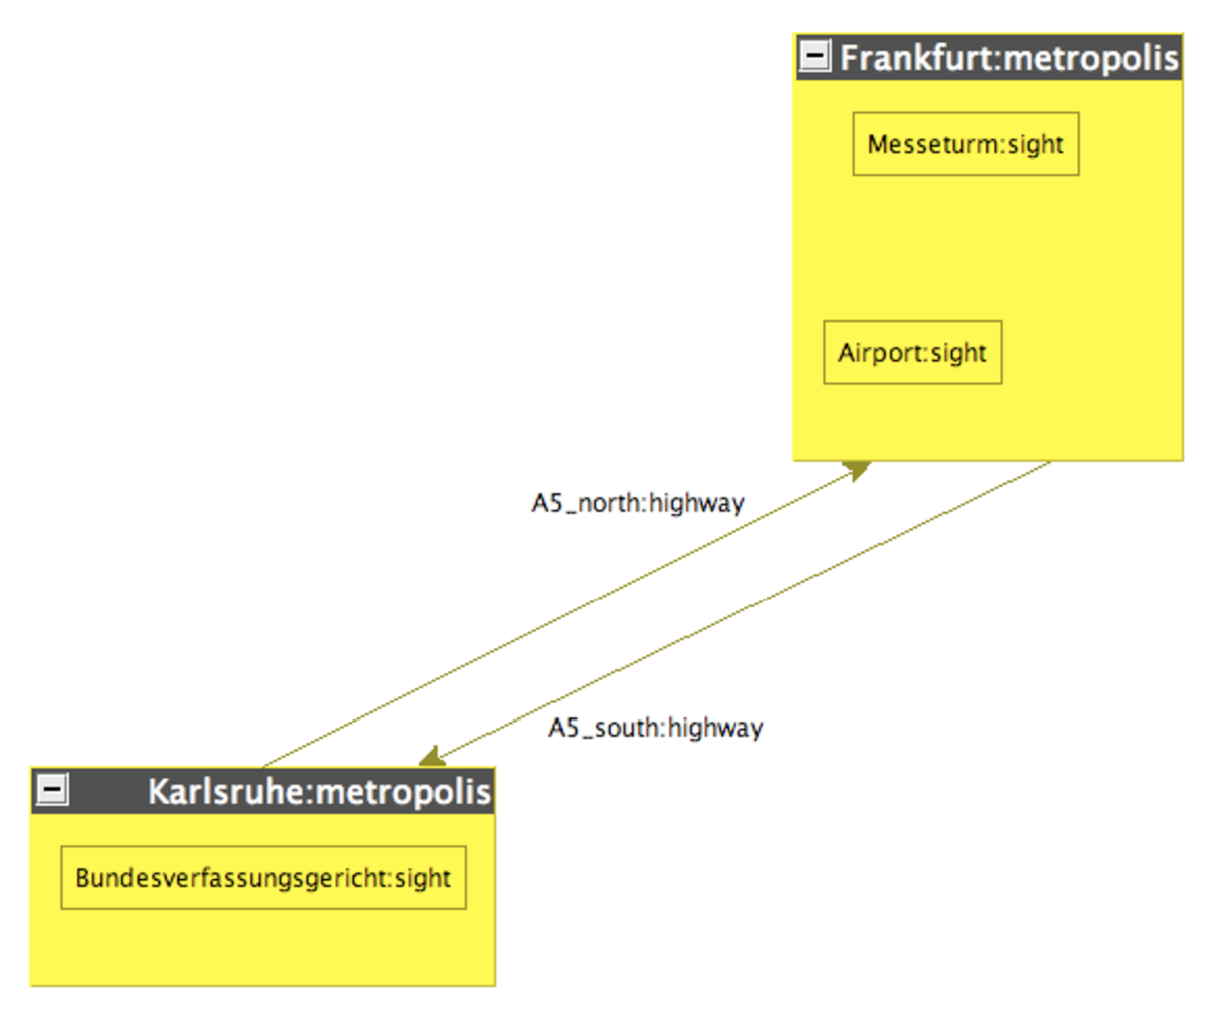
\includegraphics[width=0.45\linewidth]{fig/group2-2}}\\
  {\small right side: dumped with \texttt{dump add node metropolis group}}
\end{center}

\begin{rail}
  'dump' 'add' (() | 'only') ('node' NodeType | 'edge' EdgeType) \\ ('infotag' | 'shortinfotag') AttributeName
\end{rail}\ixkeyw{dump}\ixkeyw{add}\ixkeyw{only}\ixkeyw{node}\ixkeyw{edge}\ixkeyw{infotag}\ixkeyw{shortinfotag}
Declares the \indexed{attribute} \emph{AttributeName} to be an ``\indexed{info tag}'' or ``\indexed{short info tag}''.
Info tags are displayed like additional node/edge \indexed{label}s, in format \texttt{Name=Value}, or \texttt{Value} only for short info tags.
The keyword \texttt{only} excludes the subtypes of \emph{NodeType} resp.\ \emph{EdgeType}.
In the following example \emph{river} and \emph{jam} are info tags:
\begin{center}
  \fbox{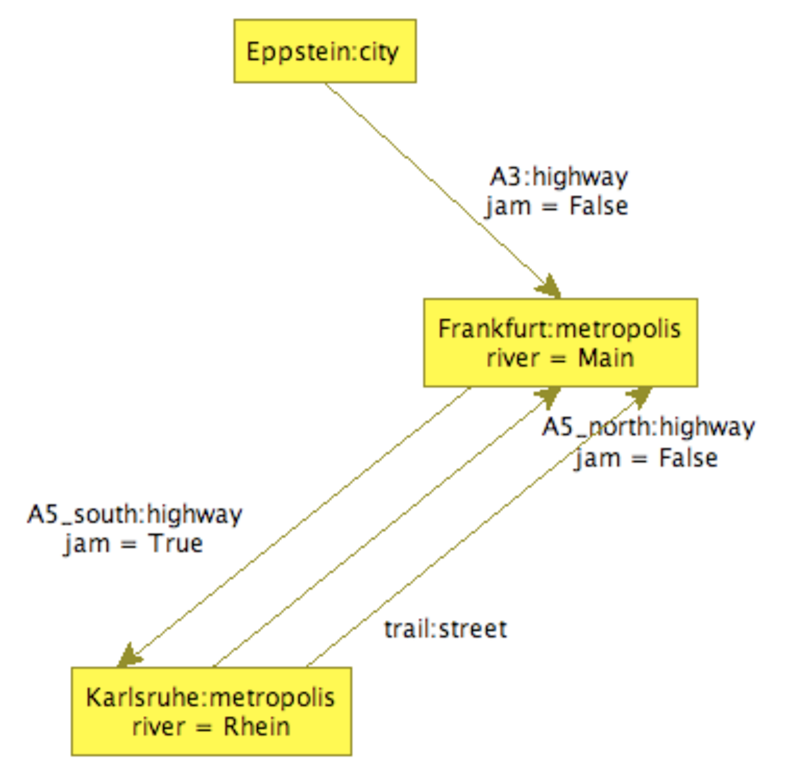
\includegraphics[width=0.5\linewidth]{fig/infotag}}
\end{center}

\begin{rail}
  'dump' 'add' 'graph' 'exclude';
  'dump' 'set' 'graph' 'exclude' 'option' ContextDepth;  
\end{rail}\ixkeyw{dump}\ixkeyw{add}\ixkeyw{graph}\ixkeyw{exclude}\ixkeyw{option}
The dump graph exclude commands allow to suppress the display of the graph during debugging. Instead only the match of the current rule is shown, plus some context up do a certain depth, plus the parent nodes according to the nesting commands. The default depth is 1, i.e. the match plus its direct neighbours are displayed (plus the nesting nodes); you may set it to 0 or a higher value. These commands allow you to still use the debugger if the graph as such is too large to be layed out (or laying it out takes too long to be convenient).

\begin{rail}
  'dump' 'reset'
\end{rail}\ixkeyw{dump}\ixkeyw{reset}
Resets all style options (\texttt{dump set}\dots) and (\texttt{dump add}\dots) to their default values.


\begin{note}\label{note:visual}
Small graphs allow for fast visual understanding, but with an increasing number of nodes and edges they quickly loose this property.
The group commands are of outstanding importance to keep readability with increasing graph sizes
(e.g. for program graphs it allows to lump together expressions of a method inside the method node and attributes of the class inside the class node).
Additional helpers in keeping the graph readable are:
the capability to exclude elements from dumping (the less hay in the stack the easier to find the needle),
the different colors and shapes to quickly find the elements of interest,
as well as the labels/infotags/shortinfotags to display the most important information directly.
Choose the layout algorithm and the options delivering the best results for your needs, organic and hierarchic or compiler graph
(an extension of hierarchic with automatic edge cutting -- marking cut edges by fat dots, showing the edge only on mouse over and allowing to jump to the other end on a mouse click)
should be tried first.
\end{note}

The following example shows several of the layout options employed to considerably increase the readability of a program graph (as given in \texttt{examples/JavaProgramGraphs-GraBaTs08}):
\begin{figure}[htbp]
  \centering
  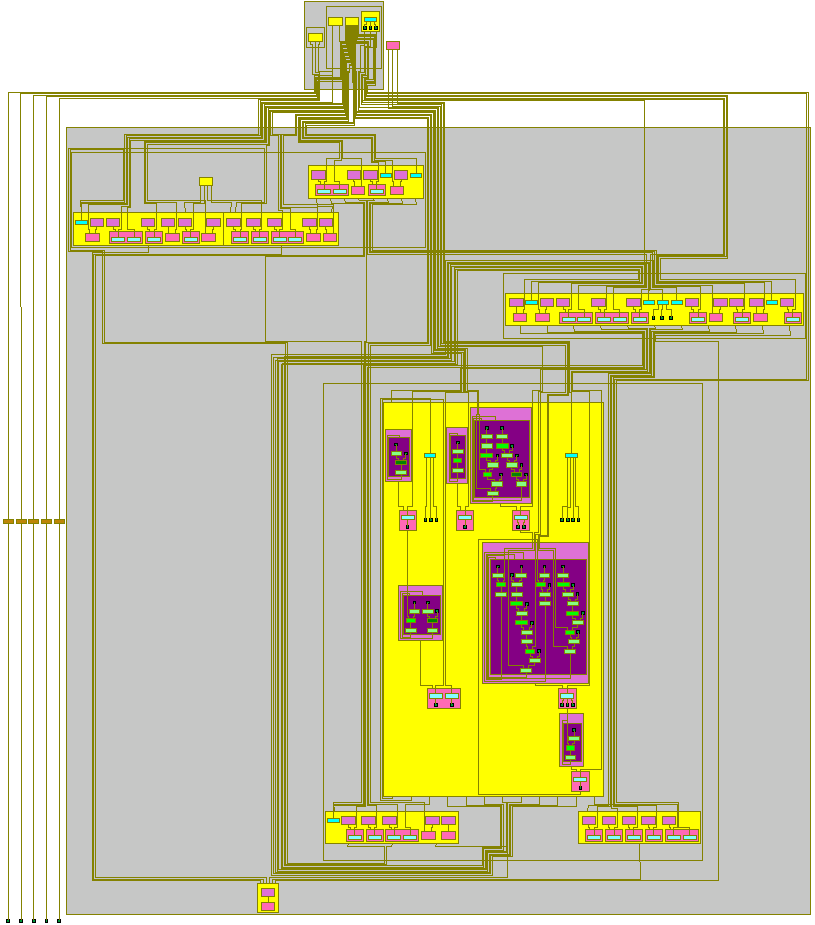
\includegraphics[width=0.99\textwidth]{fig/screen-overview}
  \caption{Overview of the initial program graph }
  \label{figprogramgraph1}
\end{figure}

\begin{figure}[htbp]
  \centering
  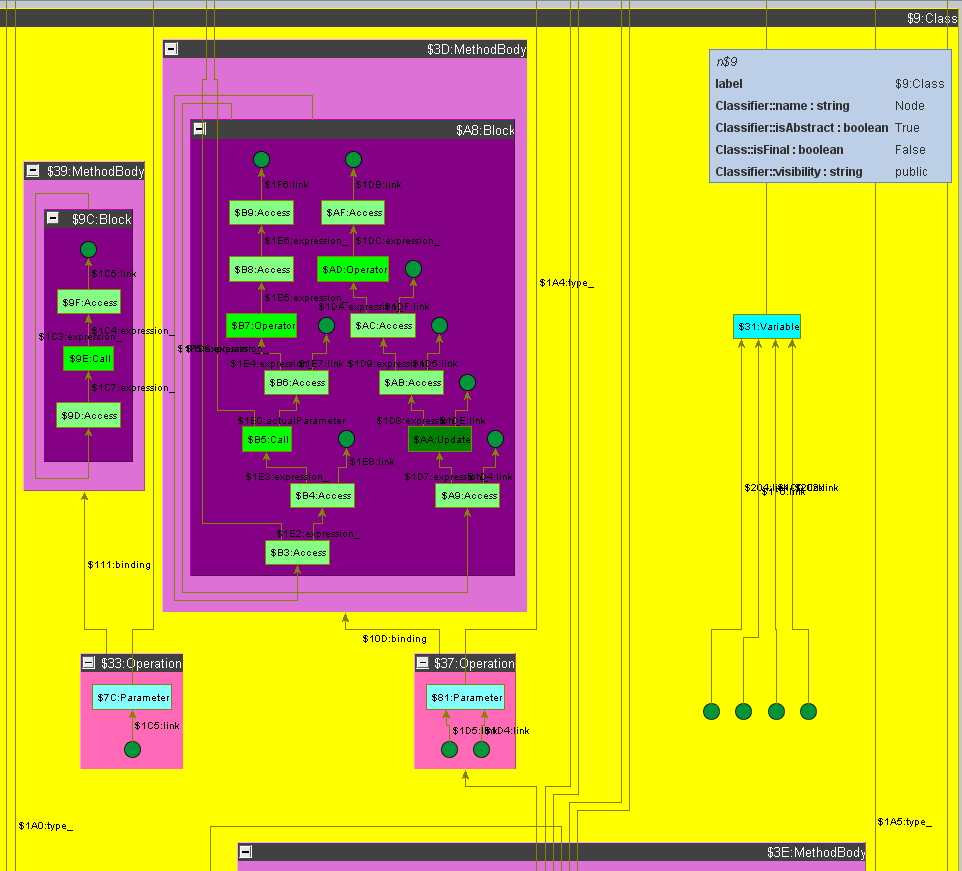
\includegraphics[width=0.99\textwidth]{fig/screen-detail}
  \caption{Some details of the ``Node'' class of the initial program graph}
  \label{figprogramgraph2}
\end{figure}

\pagebreak 


%%%%%%%%%%%%%%%%%%%%%%%%%%%%%%%%%%%%%%%%%%%%%%%%%%%%%%%%%%%%%%%%%%%%%%%%%%%%%%%%%%%%%%%%%%%%%%%%
\section{yComp Usage}

\yComp\indexmain{yComp} \cite{ycomp} is the default graph viewer of GrGen, and -- when started as a server process -- can be controlled by the debugger of GrShell via a TCP/IP connection.
Besides the things already mentioned in \ref{tools:ycomp}, we want to give the following hints:
\begin{itemize}
	\item when started on a dump, you must press the rightmost play button to start layout
	\item play with the layout options offered in the \texttt{Layout} menu until you find a good visualization, configure it then in the GrShell; don't forget to press the play button to apply the changes
	\item you can pane by pressing and holding the middle mouse button while moving the mouse
	\item you can zoom with the mouse wheel at the position of the cursor
	\item hovering over graph elements displays the attributes
	\item you can select graph elements with the left mouse button and delete them with \texttt{del} to gain a better overview
	\item by activating edit mode with the 3rd rightmost button you can move nodes around, which allows you to fix a bad layout (rather seldom needed)
	\item the context menu opened by pressing the right mouse button over a graph element allows you to explore the adjacent nodes in non-edit-mode, or delete the element in edit mode
	\item you can search with \texttt{Ctrl-f} or \texttt{/} for the persistent name or an attribute value (or by clicking into the left search field), the matching elements get highlighted
\end{itemize}


%%%%%%%%%%%%%%%%%%%%%%%%%%%%%%%%%%%%%%%%%%%%%%%%%%%%%%%%%%%%%%%%%%%%%%%%%%%%%%%%%%%%%%%%%%%%%%%%
\section{Debugging Related Commands}

\begin{rail}
  'debug' ( 'enable' | 'disable' )
\end{rail}\ixkeyw{debug}\ixkeyw{enable}\ixkeyw{disable}
Enables and disables the \indexed{debug mode}.
The debug mode shows the current working graph in a \yComp\ window.
All changes to the working graph are tracked by \yComp\ immediately.

\begin{rail}
  'debug' 'set' 'layout' ( (Text)? | 'option' Name String ) ;
\end{rail}\ixkeyw{debug}\ixkeyw{set}\ixkeyw{layout}\ixkeyw{option}
Sets the default graph \indexed{layout algorithm} to \emph{Text}.
If \emph{Text} is omitted, a list of the available layout algorithms is displayed.
The following layout algorithms are supported: \texttt{Random}, \texttt{Hierarchic}, \texttt{Organic}, \texttt{Orthogonal}, \texttt{Circular}, \texttt{Tree}, \texttt{Diagonal}, \texttt{Incremental Hierarchic}, \texttt{Compilergraph}.
For technical graphs \texttt{Hierarchic} works normally best; \texttt{Compilergraph} is a version of \texttt{Hierarchic} cutting some edges, it may be of interest if \texttt{Hierarchic} contains too many crossing edges. \texttt{Organic} is the other general purpose layout available, the other layouts are rather special, but this should not prevent you from using them if they fit to your task ;).
The \texttt{option} version allows to specify layout options by name value pairs.
The available layout options can be listed by the following command.

\begin{rail}
  'debug' 'get' 'layout' 'options';
\end{rail}\ixkeyw{debug}\ixkeyw{get}\ixkeyw{layout}\ixkeyw{options}
Prints a list of the available layout options of the layout algorithm.

\begin{rail}
  'debug' 'layout';
\end{rail}\ixkeyw{debug}\ixkeyw{layout}
Forces re-layout of the graph shown in yComp (same as pressing the play button within yComp).

\begin{rail}
  'debug' 'set' 'node' 'mode' Text DumpNodeContinuation ;
\end{rail}\ixkeyw{debug}\ixkeyw{set}\ixkeyw{mode}
\begin{rail}
  'debug' 'set' 'edge' 'mode' Text DumpEdgeContinuation ;
\end{rail}\ixkeyw{debug}\ixkeyw{set}\ixkeyw{mode}
Configures the display of the visual debug states for the nodes/edges.
The following modes are supported: \texttt{matched}, \texttt{created}, \texttt{deleted}, \texttt{retyped}.
Change this if you e.g. want the matched elements to be marked more visibly, or added/deleted elements to be colored green/red.

\begin{rail}
  GraphRewriteSequence: 'debug' ('exec'|'xgrs') SimpleRewriteSequence ;
\end{rail}\ixkeyw{debug}\ixkeyw{exec}\ixkeyw{xgrs}\indexmain{graph rewrite sequence}\indexmainsee{GRS}{graph rewrite sequence}\ixnterm{GraphRewriteSequence}
This executes the graph rewrite sequence \emph{SimpleRewriteSequence} in the debugger\indexmain{debugger}.
Same as \texttt{exec SimpleRewriteSequence} in the previous chapter, but allows tracing the rewriting process step-by-step.


%%%%%%%%%%%%%%%%%%%%%%%%%%%%%%%%%%%%%%%%%%%%%%%%%%%%%%%%%%%%%%%%%%%%%%%%%%%%%%%%%%%%%%%%%%%%%%%%
\section{Using the Debugger}

The debugging process follows of a series of debug situations,
which result from a user selection of the underlying execution situations according to interest.
During each debugging step the debugger\indexmain{debugger} -- which is a part of the \GrShell~--
prints the debugged sequence with the currently focused/active rule highlighted yellow.
What will be shown from executing this rule depends on the commands chosen by the user;
and on the fact whether the focused rule matches or not.
An active rule which is already known to match is highlighted green.
The rules which matched during sequence execution are shown on dark green background,
the rules which failed during sequence execution are shown on dark red background;
at the begin of a new loop iteration the highlighting state of the contained rules is reset.
During execution \yComp\footnote{Make sure, that the path to your \texttt{\indexed{yComp.jar}} package is set correctly in the \texttt{ycomp} shell script within \GrG's \texttt{/bin} directory.}\indexmain{yComp}
will display the changes to the graph from every single step.
Besides deciding on what is shown from the execution of the current rule,
the user determines with the debug commands where to continue the execution
(the rule focused next; but again this depends on success/failure of the currently active rule).
The debug commands are given in Table~\ref{tabdebug}.
A run is shown in the following example \ref{ex:debug}.

\pagebreak %manual break to get two pages with halfway broken layout instead of one with deeply broken

In addition to the commands for actively stepping or skipping through the sequence execution,
there are breakpoints and choicepoints available (toggled with the \texttt{b} and \texttt{c} commands)
which are only processed when they are reached, but on the other hand are also processed if a user command would skip them.
The \indexed{break point}s halt execution, focus the reached sequence, and cause the debugger to wait for further commands
(e.g. \texttt{d} to inspect the rule execution en detail versus \texttt{s} for just applying it).
The \indexed{choice point}s halt execution, focus the reached sequence in magenta, and ask for some user input;
after the input was received, execution continues according to the command previously issued.

Both break points and choice points are denoted by the \texttt{\%} modifier.
The \texttt{\%} modifier works as a break point if it is given before: a rule, an all bracketed rule, a variable predicate, or the constants \texttt{true}/\texttt{false}.
The \texttt{\%} modifier works as a choice point if it is appended to the \texttt{\$} randomize modifier switching a random decision into a user decision.
This holds for the binary operators, the random match selector of all bracketed rules, the random-all-of operators and the one-of-set braces.
The idea behind this is: you need some randomization for \indexed{simulation} purposes --- then use the randomize modifier \texttt{\$}.
You want to force a certain decision overriding the random decision to try out another execution path while debugging the simulation flow --- then modify the randomize modifier with the user (choice) modifier \texttt{\%}.

The initial breakpoint and choicepoint assignment is given with the \texttt{\%} characters in the sequences after the \texttt{debug exec} commands in the \texttt{.grs} file.
The breakpoint and choicepoint commands of the debugger allow to toggle them at runtime, overriding the initial assignment (notationally yielding a sequence with added or removed \texttt{\%} characters).
The user input commands \texttt{\$\%(type)} define choice points which can't be toggled off.

Further commands allow to print the variables at a given situation, the sequence call stack, or a full state dump of the call stack and the variables.
Or allow to dump the current graph, or highlight elements in the graph, defined by being contained in a (possibly container valued) variable, or being visited according to a visited flag.

\pagebreak

\begin{table}[htbp]
  \begin{tabularx}{\linewidth}{|lX|}
\hline
  \texttt{s}(tep) & Execute the current rewrite rule (match, and rewrite in case it matched; the resulting graph is shown).\\
  \texttt{d}(etailed step) & Execute the current rewrite rule in a three-step procedure: matching - highlighting the found match, rewriting - highlighting the changing elements, and application - doing the rewrite showing the resulting graph. In addition, afterwards the execution of subrules from embedded sequences (\texttt{exec}) is shown step by step. \\
  (step) \texttt{o}(ut) & Continue execution until the end of the current loop. If the execution is not in a loop at this moment, but in a sequence called, the called sequence will be executed until its end. If neither is the case, the complete sequence will be executed.\\
  (step) \texttt{u}(p) & Ascend one level up within the \indexed{Kantorowitsch tree} of the current rewrite sequence (i.e. rule; see Example~\ref{ex:debug}; at the moment the command is pretty useless because only the serialized form is displayed).\\
  \texttt{r}(un) & Continue execution (until the end or a breakpoint).\\
  \texttt{a}(bort) & Cancel the execution immediately.\\
  \texttt{n}(ext) & Go to the next rewrite rule which matches, make it current.\\
\hline
  (toggle) \texttt{b}(reakpoint) & Toggle a breakpoint at one of the breakpointable locations.\\
  (toggle) \texttt{c}(choicepoint) & Toggle a choicepoint at one of the choicepointable locations.\\
	(edit) \texttt{w}(atchpoints) & Allows to edit data breakpoints or the behaviour for programmed debug messages.\\
\hline
  \texttt{v}(ariables) & Prints the global variables and the local variables of the sequence currently executed, which is the topmost sequence of the sequence call stack. Plus the allocated visited flags. To be more precise regarding local variables: all variables which were defined (and have not fallen out of scope again) up to the sequence position focussed.\\
  \texttt{t}(race) & Prints the stack trace of the current sequence call stack; the stack trace includes the body of each sequence called at its execution state.\\
  \texttt{f}(ull dump) & Prints the stack trace including the local variables of each stack frame plus the global variables.\\
  (dum)\texttt{p} (graph)\label{dumpgraph} & Dumps the current graph as a \texttt{.vcg} file and shows it in yComp. This can be used as a workaround to check the real state in case transaction/backtracking rollback is used on a graph with node nesting, which may lead to a buggy display.\\
  (as)-\texttt{g}(raph) & Asks for the value of the externally defined type that is to be shown in the debugger in graph form (you must implement an extension handler able to return an \texttt{INamedGraph} on request for this to work, see \ref{sub:apiextemitparse}). Alternatively, you may specify a graph value, which is then displayed directly.\\
  \texttt{h}(ighlight)\label{highlight} & Highlights the elements in the graph which are marked with the visited flag given, or are contained in the variable given (which might be a simple scalar variable containing a graph element, or a container variable). Multiple variables or visited flags may be given separated by commas.\\
\hline
  \end{tabularx}
  \caption{\GrShell\ debug commands}
  \label{tabdebug}
\end{table}
%\begin{figure}[htbp]
%  \centering
%  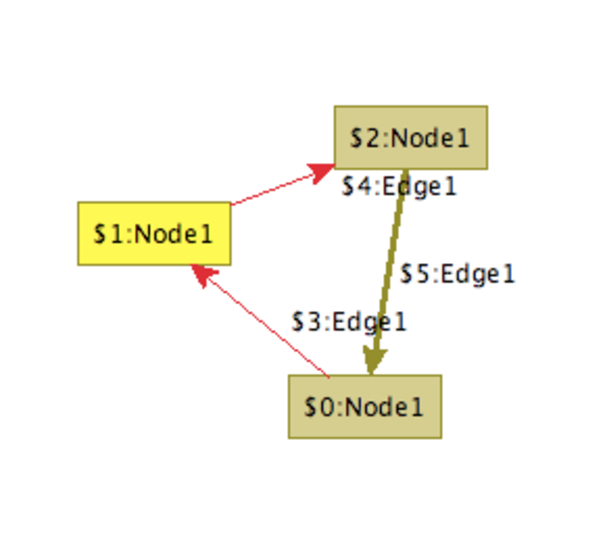
\includegraphics[width=0.25\linewidth]{fig/debug1}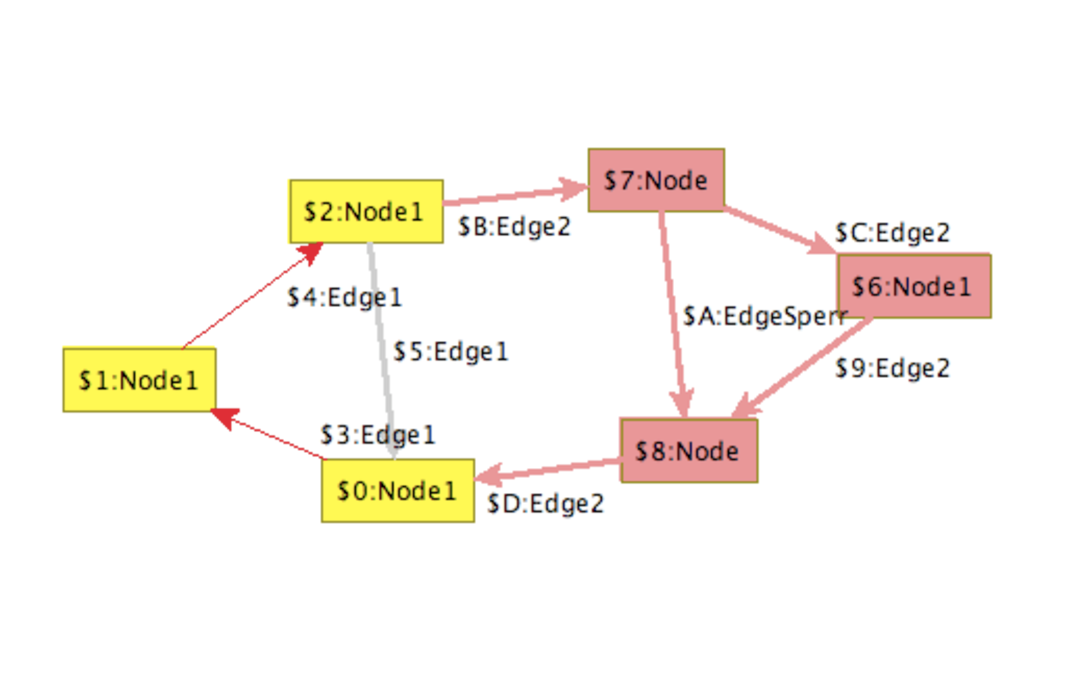
\includegraphics[width=0.4\linewidth]{fig/debug2}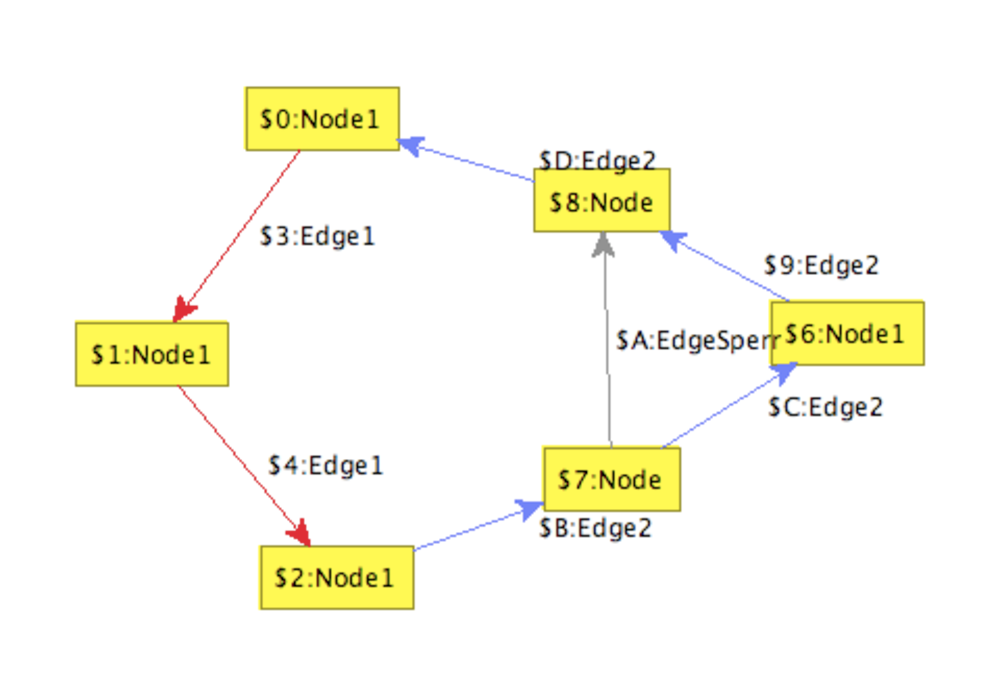
\includegraphics[width=0.4\linewidth]{fig/debug3}
%  \caption{Delayed step rule application.}
%  \label{figdebug}
%\end{figure}

\pagebreak

\begin{figure}[htbp]
\begin{example}\label{ex:debug}
We demonstrate the debug commands with a slightly adjusted script for the Koch snowflake from \GrG's examples (see also Section~\ref{fractals}). The graph rewriting sequence is
\begin{grshell}
debug exec (makeFlake1* & (beautify & doNothing)* & makeFlake2* & beautify*)[1]
\end{grshell}
\yComp\ will be opened with an initial graph (resulting from \texttt{grs init}):
\begin{center}
  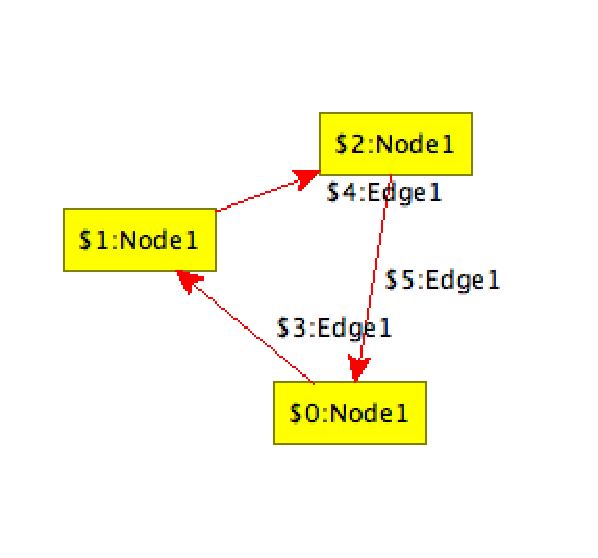
\includegraphics[width=0.3\linewidth]{fig/debug0tra}
\end{center}
We type \texttt{d}(etailed step) to apply \texttt{makeFlake1} step by step resulting in the following graphs:
\begin{center}
  \parbox{0.2\linewidth}{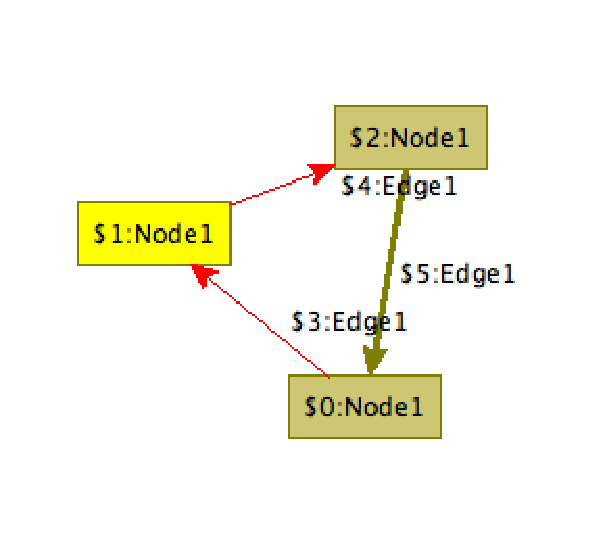
\includegraphics[width=\linewidth]{fig/debug1tra}}\parbox{0.375\linewidth}{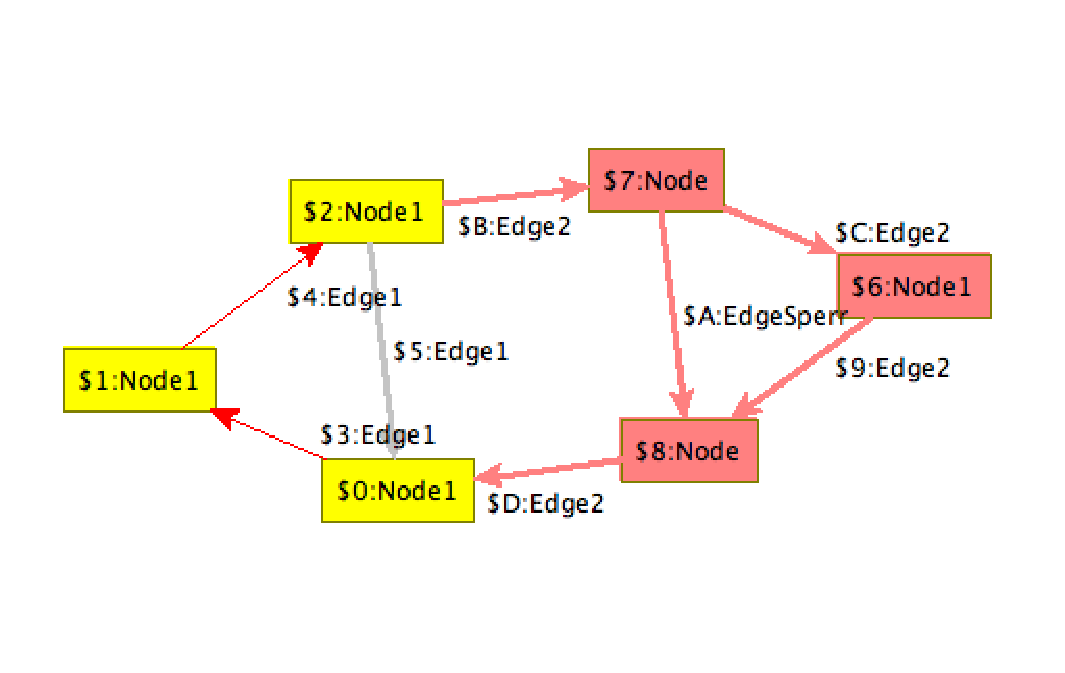
\includegraphics[width=\linewidth]{fig/debug2tra}}\parbox{0.375\linewidth}{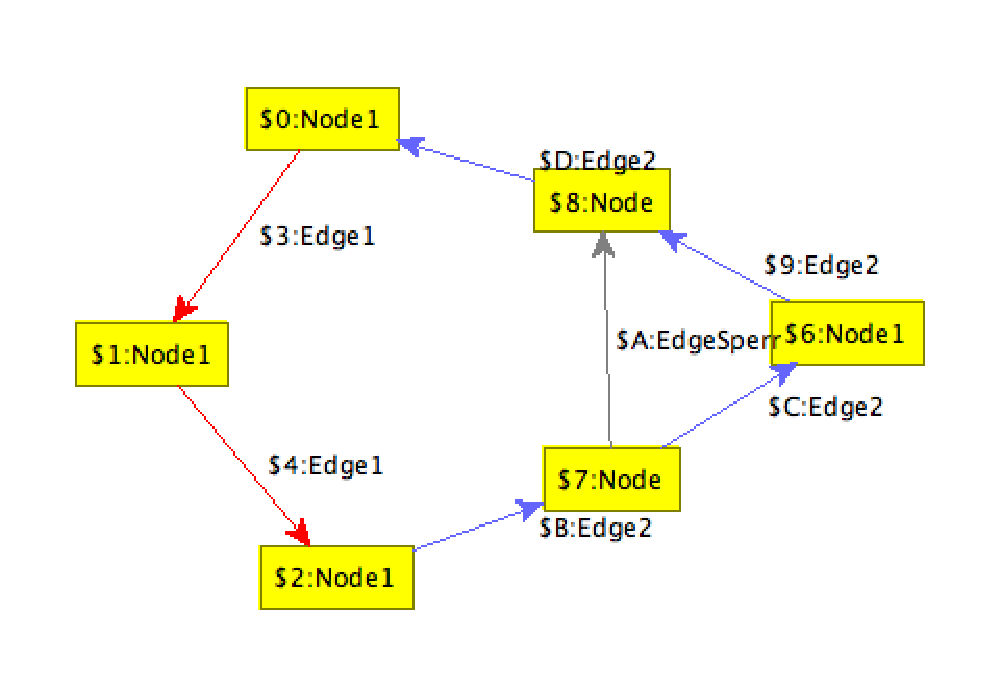
\includegraphics[width=\linewidth]{fig/debug3tra}}
\end{center}
The following table shows the ``break points'' of further debug commands, entered one after another:
\begin{center}
  \begin{tabular}{|l|l|} \hline
    \textbf{Command} & \textbf{Active rule} \\ \hline
    \texttt{s} & \texttt{makeFlake1} \\
    \texttt{o} & \texttt{beautify} \\
    \texttt{s} & \texttt{doNothing} \\
    \texttt{s} & \texttt{beautify} \\
    \texttt{u} & \texttt{beautify} \\
    \texttt{o} & \texttt{makeFlake2} \\
    \texttt{r} & --- \\ \hline
  \end{tabular}
\end{center}
\end{example}
\end{figure}

%\subsection{yComp}
%url; yFiles; java app, socket communication with shell debugger
%Find; goto node/edge; b�bbels;
%relayout; zoom: mousewheel; pane by holding middle mouse
%supported formats; vcg format
%ref to visualization commands, again: hierarchy
%copy some of the stuff from ycomp help?

\pagebreak

%%%%%%%%%%%%%%%%%%%%%%%%%%%%%%%%%%%%%%%%%%%%%%%%%%%%%%%%%%%%%%%%%%%%%%%%%%%%%%%%%%%%%%%%%%%%%%%%
\section{Subrule Debugging and Programmed Halts}\label{secdebuggersubrule}

The basic granularity of debugging in \GrG{} is the single rule called from an interpreted sequence.
But with embedded execs there are further sequences and actions available outside direct control and visibility of the debugger.
At least the actions called from the embedded sequences are shown in the debugger -- in case detailed mode is used.
But the local execution state of imperative code which may be used for tasks where pattern matching is not benefitial is completely invisible to the debugger.
Only the effects on the graph become visible.

There is a remedy for this situation, code-embedded debugging commands, in the form of calls to procedures from the built-in package \texttt{Debug}.
With them you can punch holes into the covering blanket that allow you to peek at what's going on under the covers.
The debugging commands are used for one to directly display information, but for the other for handling a stack of debug messages, intended for representing the current state of the call nesting of the executing code.

The available commands are:
\begin{description}
\item[\texttt{Debug::add(message(,object)*)}] to be called when a subrule computation or an interesting piece of code is entered.
The message is added to the debug messages stack of the debugger.
Besides the mandatory \texttt{message:string}, an arbitrary number of other parameters may be given (of arbitrary type).
\item[\texttt{Debug::rem(message(,object)*)}] to be called when a subrule computation or an interesting piece of code is exited.
The topmost entry message on the messages stack is removed.
It is checked that the message of the topmost added entry is identical to the message of current removal -- you must always call \texttt{add} and \texttt{rem} in pairs!
The \texttt{emit} messages on the way to the topmost \texttt{add} are removed. Besides the mandatory \texttt{message:string}, an arbitrary number of other parameters may be given (of arbitrary type).
\item[\texttt{Debug::emit(message(,object)*)}] to be called when some interesting points in the code are passed.
The message is added to the debug messages stack of the debugger.
Besides the mandatory \texttt{message:string}, an arbitrary number of other parameters may be given (of arbitrary type).
\item[\texttt{Debug::halt(message(,object)*)}] to be called when some point in the code is reached that is so interesting that you want the execution to break in the debugger. 
If called, the debugger halts execution, displays the messages stack in its current state, and prints out the halt message with its parameters.
Besides the mandatory \texttt{message:string}, an arbitrary number of other parameters may be given (of arbitrary type).
\item[\texttt{Debug::highlight(message(,object,string)*)}] to be called when some point in the code is reached that is so interesting that you want the execution to break in the debugger, in order to display some variable values highlighted graphically in the debugger, in the same way they are highlighted when an action is matched.
If called, the debugger halts execution, displays the messages stack in its current state, and displays the nodes and edges passed with the additional parameters highlighted in the graph.
The additional parameters must be given in pairs, first the entity to display, then the string that entry will be annotated with in the debugger.
The entity to display may be a node or edge, which is then directly highlighted,
or a storage containing nodes or edges, all contained nodes/edges will then be highlighted,
or a visited flag (integer number), all graph elements that are visited according to that flag are then highlighted.
Besides, as first mandatory parameter, the \texttt{message:string} must be given.
\end{description}

Some \texttt{add} and \texttt{rem} are automatically inserted by \GrG{} for you.
For one for embedded execs, a debug message is sent when an embedded exec is entered or exited, with a message starting with the name of the containing rule.
For the other for procedures and compiled sequence definitions, a debug message is sent when a procedure or defined sequence is entered or exited, with a message being equal to the name of the procedure or defined sequence.

%%%%%%%%%%%%%%%%%%%%%%%%%%%%%%%%%%%%%%%%%%%%%%%%%%%%%%%%%%%%%%%%%%%%%%%%%%%%%%%%%%%%%%%%%%%%%%%%
\section{Watchpoint configuration}

The behaviour of the debugger upon receiving certain events can be defined with configuration rules or watchpoints.
When a subrule debugging event (aka debug message), or a graph change event, or an action match event occurs,
is the list visited one entry after the other, and one configuration rule checked for a match.
When a configuration rule or watchpoint matches, is its decision applied.
The decision may be to break execution and display the current execution state, or to continue execution, which is of interest for events that normally break execution but should be better ignored.

Besides defining the configuration rules of the watchpoints beforehand with shell commands, can you edit them interactively with the edit \texttt{w}atchpoint command inside the debugger. 

\subsection*{Subrule messages}

\begin{rail}
  'debug' 'on' ('add'|'rem'|'emit') MessageFilter 'break';
  'debug' 'on' ('halt'|'highlight') MessageFilter 'continue';
	MessageFilter: ('equals' | 'startsWith' | 'endsWith' | 'contains') '(' StringConstant ')';
\end{rail}\ixkeyw{debug}\ixkeyw{on}\ixkeyw{add}\ixkeyw{rem}\ixkeyw{emit}\ixkeyw{halt}\ixkeyw{highlight}\ixkeyw{break}\ixkeyw{continue}\ixnterm{MessageFilter}\ixkeyw{equals}\ixkeyw{startsWith}\ixkeyw{endsWith}\ixkeyw{contains}

When the string specified matches the message of the debug event according to the message filter given,
is execution interrupted by the debugger in case of an \texttt{Debug::add}, \texttt{Debug::rem}, \texttt{Debug::emit}
which normally occurs silently, those events are typically only used to represent the execution state of the code in the debugger.
When a match happens for a \texttt{Debug::halt} or \texttt{Debug::highlight} is execution continued without interruption, while normally those messages break execution in the debugger.

\subsection*{Action match event}

\begin{rail}
  'debug' 'on' 'match' RuleName ('break'|'continue') ('if' SequenceExpression)?;
\end{rail}\ixkeyw{debug}\ixkeyw{on}\ixkeyw{match}\ixkeyw{break}\ixkeyw{continue}\ixkeyw{if}

When the action specified was matched, is execution halted in the debugger in case of a \texttt{break}.
This is of interest for rules executed from execs, as normal breakpoints don't apply to them, this way we can set a breakpoint on a rule irrespective from where it is called (allowing us to just \texttt{r}un a sequence until an action match of interest happens).
In case of a \texttt{continue} is execution forced to continue.
This is of interest for detail mode debugging that normally breaks on each matched rule.
It allows us to leave out uninteresting rules from detail mode debugging, to skip over rules in execs without the need to acknowledge them.

The sequence expression finally allows us to decide conditionally.
It is evaluated when the configuration rule is evaluated because its event occured, if it returns true the configuration rule matches, otherwise it does not match.
The \texttt{this} entity is overloaded for the sequence expression (normally it denotes the graph).
It gives access to the match found, you can access the entities of the match in dot-Notation (e.g. \texttt{this.node1}).
The configuration rule is evaluated for all matches in case of an all-bracketed match, if one returns true, the decision is carried out.

\subsection*{Graph change events}

\begin{rail}
  'debug' 'on' ('new'|'delete'|'retype'|'set' 'attributes') TypeNameSpec 'break' \\ ('if' SequenceExpression)?;
	TypeNameSpec: ('only')? Type | railat '(' Name')';
\end{rail}\ixkeyw{debug}\ixkeyw{on}\ixkeyw{new}\ixkeyw{delete}\ixkeyw{retype}\ixkeyw{set}\ixkeyw{attributes}\ixkeyw{break}\ixnterm{TypeNameSpec}\ixkeyw{only}\ixkeyw{if}

When the graph change specified occured (its corresponding event was fired), is execution halted in the debugger.
The supported graph changes are graph element creation, deletion, retyping, or attribute assignment.
The \emph{TypeNameSpec} constrains this by type or by name.
The first form matches only when the element is of the specified type, in case of \texttt{only} only if it is of exactly that type and not a subtype.
The second form matches only when the element is of the specified name, given as string constant (rules of that kind are typically created interactively, but due to the persistence of persistent names and the execution of GrGen being as deterministic as possible in between single runs make even static rules sense -- even more so if you assign the names on your own).

The sequence expression finally allows us to decide conditionally.
It is evaluated when the configuration rule is evaluated because its event occured, if it returns true the configuration rule matches, otherwise it does not match.
The \texttt{this} entity is overloaded for the sequence expression (normally it denotes the graph).
It gives access to the node or edge that was just created, is getting deleted, is getting retyped, or was assigned to.
So here we find support for conditional data breakpoints.


\chapter{Examples}
\label{anexample}

%%%%%%%%%%%%%%%%%%%%%%%%%%%%%%%%%%%%%%%%%%%%%%%%%%%%%%%%%%%%%%%%%%%%%%%%%%%%%%%%%%%%%%%%%%%%%%%%
\section{Fractals}\indexmain{example}
\label{fractals}
The \GrG\ package ships with samples for fractal generation. We will construct the \indexed{Sierpinski triangle} and the \indexed{Koch snowflake}. They are created by consecutive rule applications starting with the initial host graphs
\begin{center}
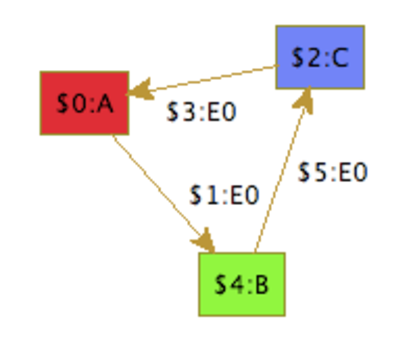
\includegraphics[width=4cm]{fig/startsir}\quad\quad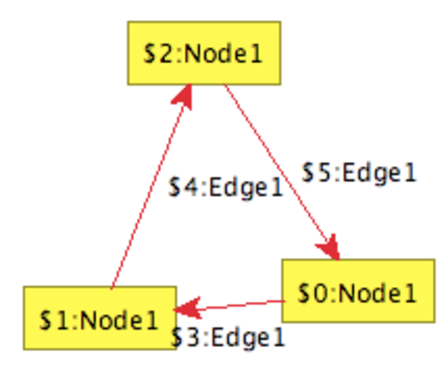
\includegraphics[width=4cm]{fig/startkoch}
\end{center}
for the Sierpinski triangle resp.\ the Koch snowflake.
First of all we have to compile the model and rule set files. So execute in \GrG's \texttt{bin} directory
\begin{verbatim}
GrGen.exe ..\specs\sierpinski.grg
GrGen.exe ..\specs\snowflake.grg
\end{verbatim}
or
\begin{verbatim}
mono GrGen.exe ../specs/sierpinski.grg
mono GrGen.exe ../specs/snowflake.grg
\end{verbatim}
respectively. If you are on a Unix-like system you have to adjust the path separators of the \GrShell\ scripts. Just edit the first three lines of \texttt{/test/Sierpinski.grs} and \texttt{/test/Snowflake.grs}. And as we have the file \texttt{Sierpinski.grs} already opened, we can increase the number of iterations to get even more beautiful graphs\footnote{Be careful: The running time increases exponentially in the number of iterations.}. Just follow the comments. Be careful when increasing the number of iterations of Koch's snowflake---\yComp's \indexed{layout algorithm} might need some time and attempts to layout it nicely.
We execute the Sierpinski script by
\begin{verbatim}
GrShell.exe ..\test\Sierpinski.grs
\end{verbatim}
or
\begin{verbatim}
mono GrShell.exe ../test/Sierpinski.grs
\end{verbatim}
respectively. Because both of the scripts are using the debug mode, we complete execution by typing \texttt{r}(un). See Section~\ref{grsthings} for further information. The resulting graphs should look like Figures~\ref{figsierp} and~\ref{figsnowflake}.
\begin{figure}[htbp]
  \centering
  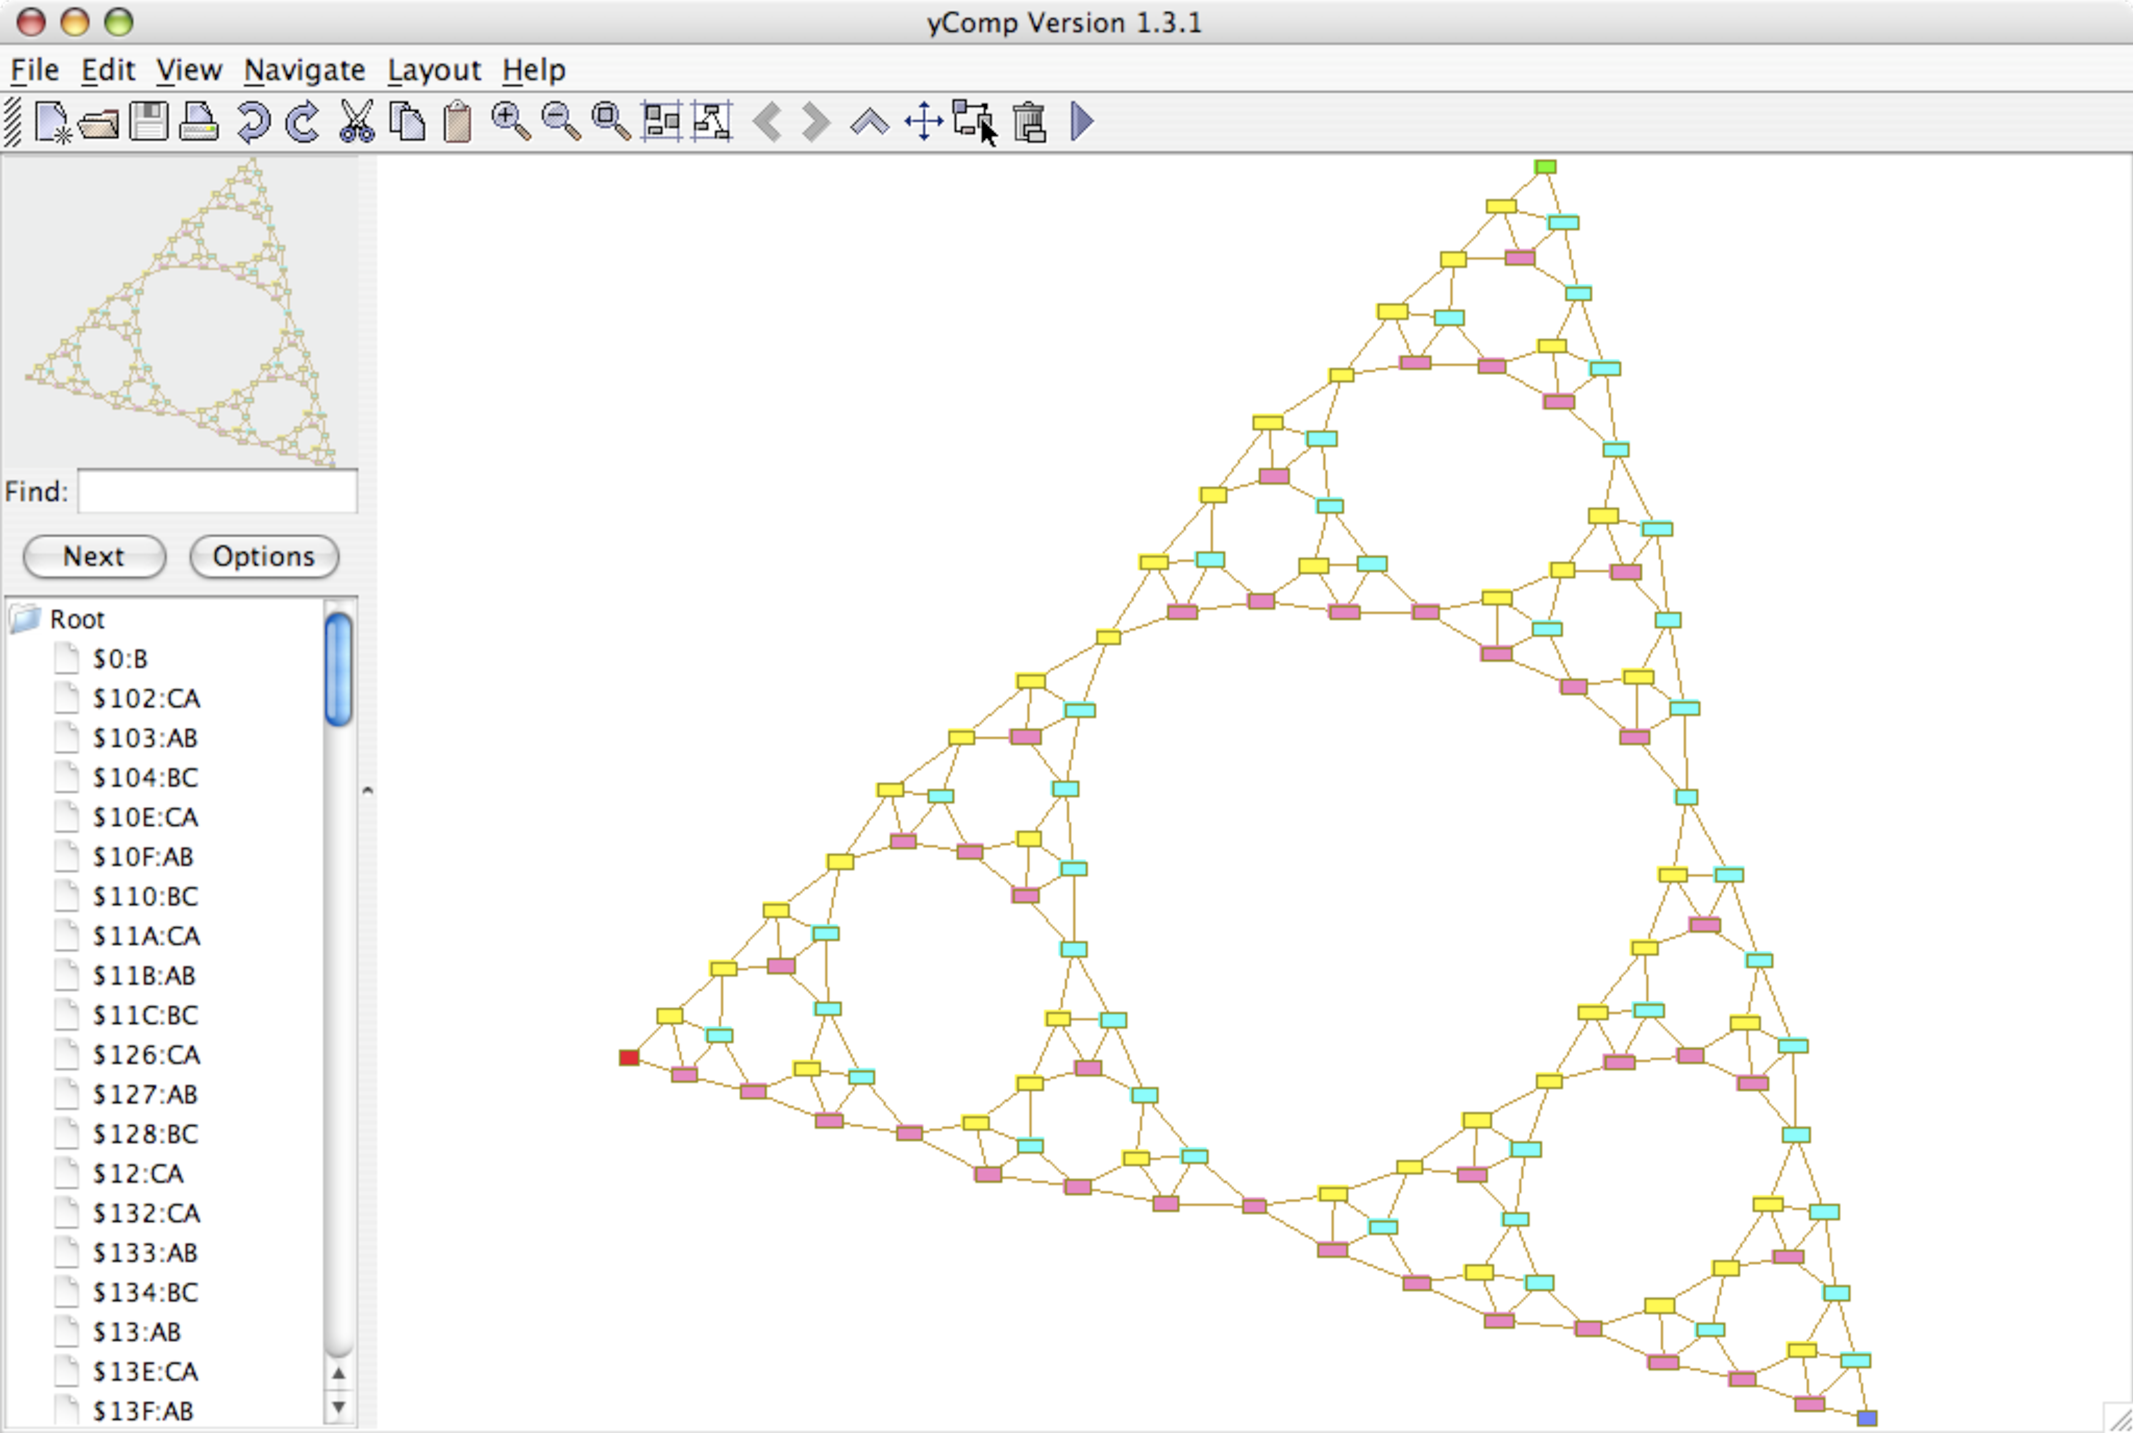
\includegraphics[width=\textwidth]{fig/sierpinski}
  \caption{Sierpinski triangle}
  \label{figsierp}
\end{figure}
\begin{figure}[htbp]
  \centering
  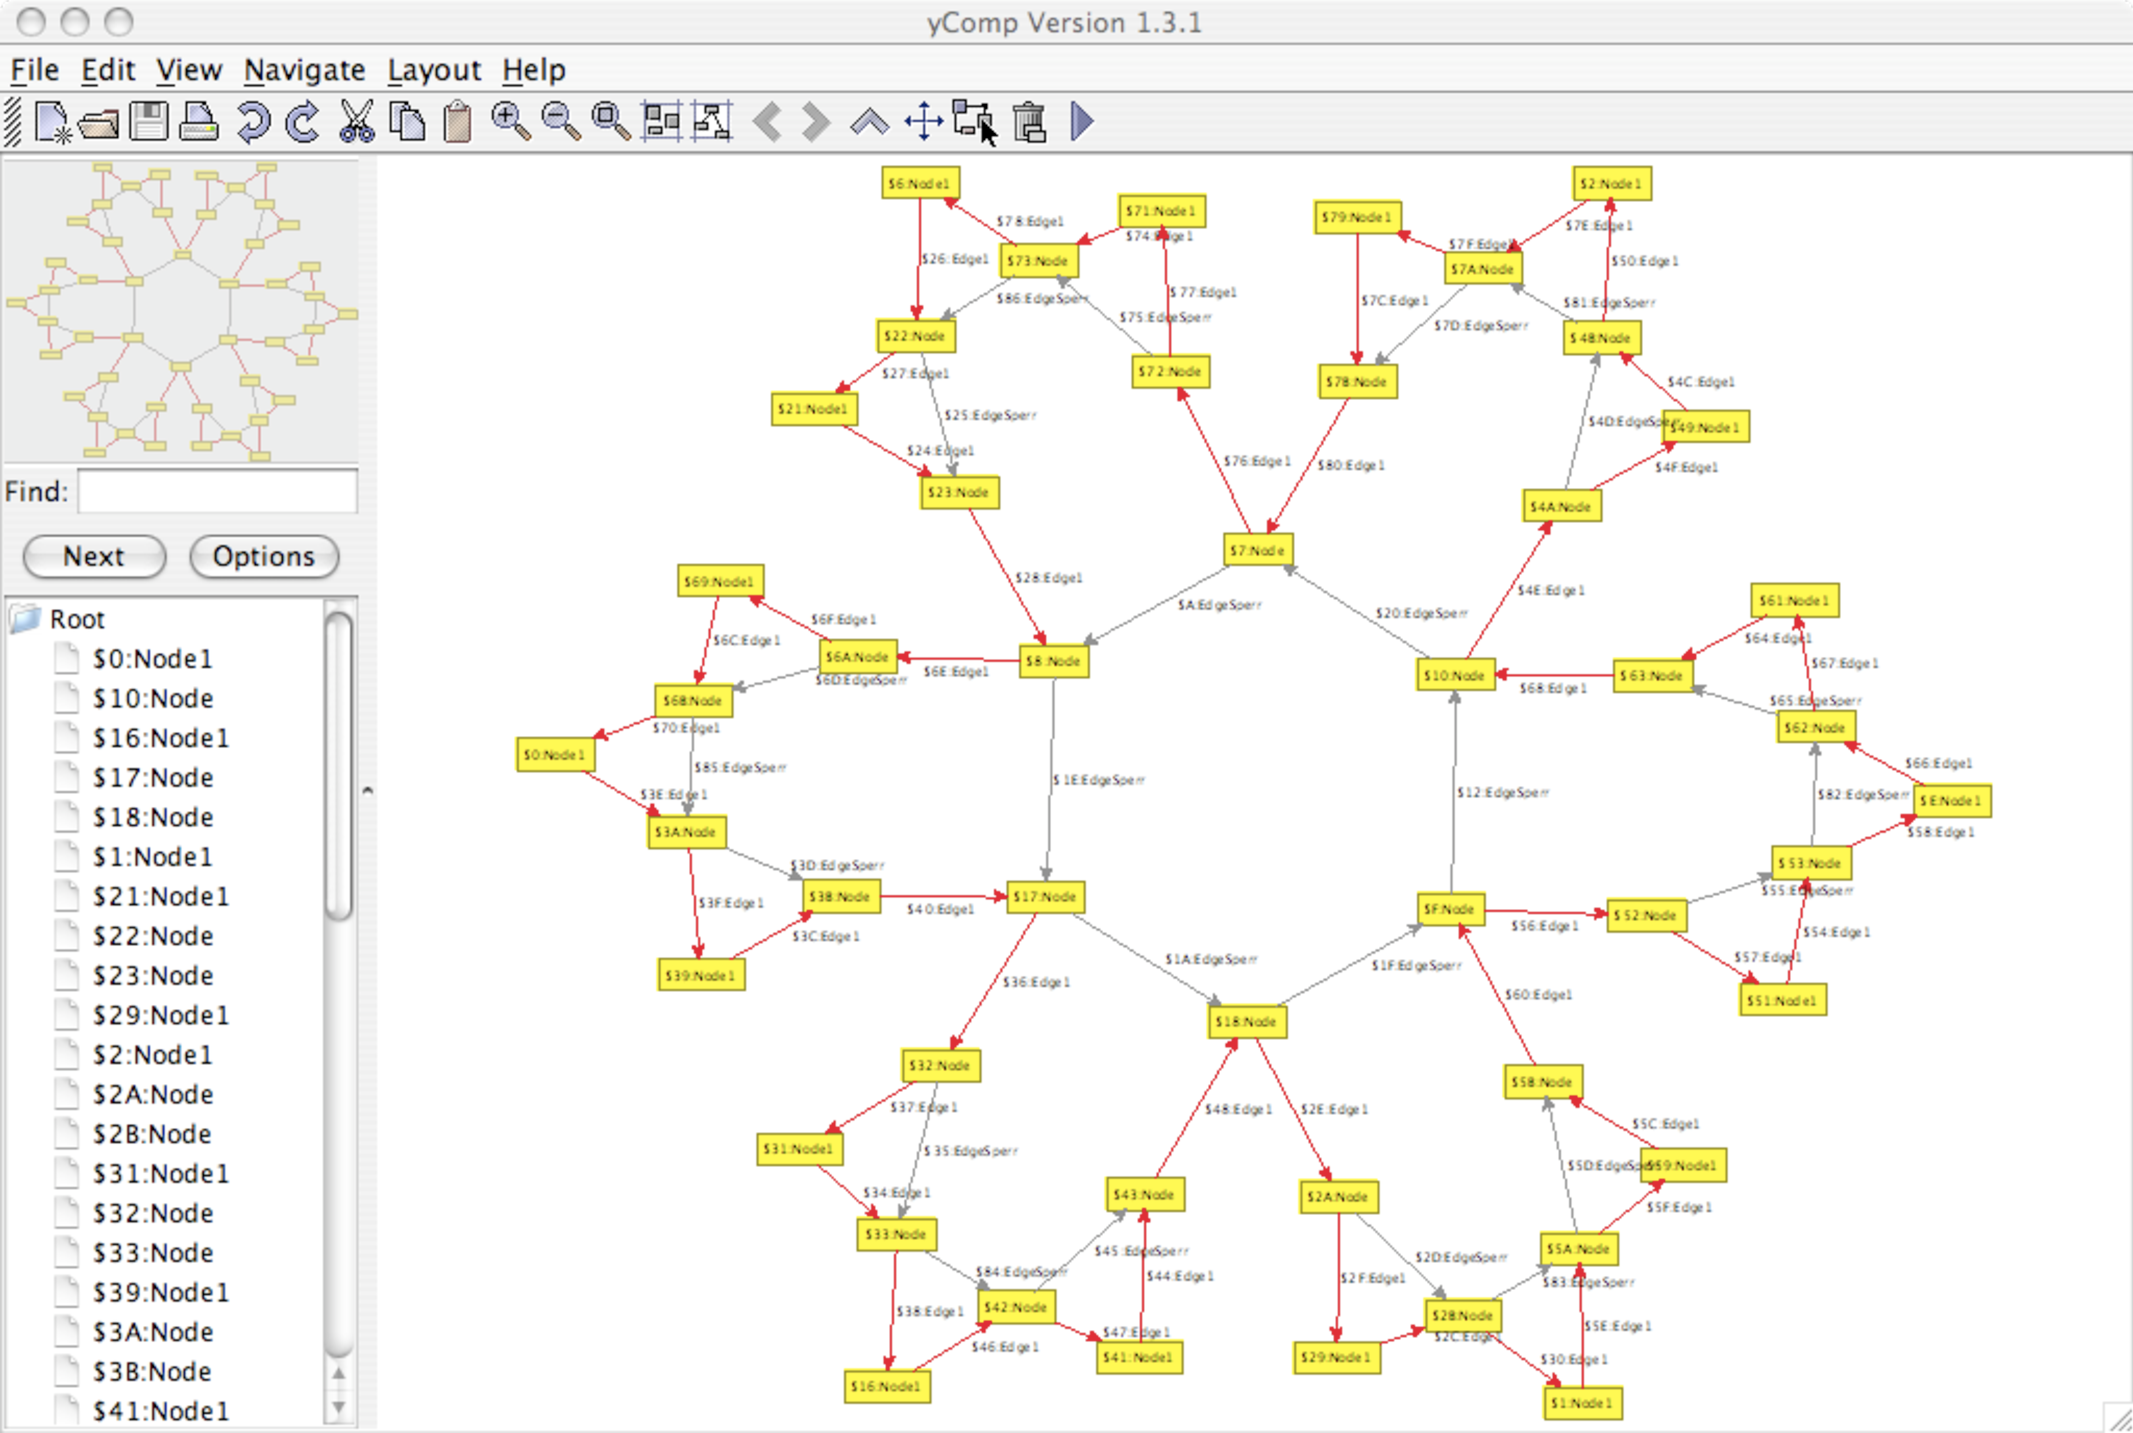
\includegraphics[width=\textwidth]{fig/snowflake}
  \caption{Koch snowflake}
  \label{figsnowflake}
\end{figure}
\vfill\pagebreak


%%%%%%%%%%%%%%%%%%%%%%%%%%%%%%%%%%%%%%%%%%%%%%%%%%%%%%%%%%%%%%%%%%%%%%%%%%%%%%%%%%%%%%%%%%%%%%%%
\section{Busy Beaver}\indexmain{example}
We want \GrG\ to work as hard as a \indexed{busy beaver}~\cite{Kro:07,Dew:84}. Our busy beaver is a Turing machine that has got five states plus a ``halt''-state; it writes 1,471 bars onto the tape and terminates~\cite{MB:00}. So first of all we design a Turing machine as graph model. Besides, this example shows that \GrG\ is \indexed{Turing complete}.

We use the graph model and the rewrite rules to define a general Turing machine. Our approach is to basically draw the machine as a graph. The busy beaver logic is implemented by rule applications in \GrShell.

%-----------------------------------------------------------------------------------------------
\subsection{Graph Model}
The tape will be a chain of \texttt{TapePosition} nodes connected by right edges. A cell value is modeled by a reflexive \texttt{value} edge, attached to a \texttt{TapePosition} node. The leftmost and the rightmost cells (\texttt{TapePosition}) do not have an incoming and outgoing edge respectively. Therefore we have the node constraint $[0:1]$.
\begin{grgen}[firstnumber=last]
node class TapePosition;
edge class right
  connect TapePosition[0:1] --> TapePosition[0:1];

edge class value
  connect TapePosition[1] --> TapePosition[1];
edge class zero  extends value;
edge class one   extends value;
edge class empty extends value;

\end{grgen}
Furthermore we need states and transitions.
The machine's current configuration is modeled with a \texttt{RWHead} edge pointing to a \texttt{TapePosition} node.
\texttt{State} nodes are connected with \texttt{WriteValue} nodes via \texttt{value} edges, a \texttt{moveLeft}/\texttt{moveRight}/\texttt{dontMove} edge leads from a \texttt{WriteValue} node to the next state (cf.~the picture on page \pageref{fig:bbstart}).
\begin{grgen}[firstnumber=last]
node class State;

edge class RWHead;

node class WriteValue;
node class WriteZero extends WriteValue;
node class WriteOne extends WriteValue;
node class WriteEmpty extends WriteValue;

edge class moveLeft;
edge class moveRight;
edge class dontMove;
\end{grgen}

%-----------------------------------------------------------------------------------------------
\subsection{Rule Set}
Now the rule set: We begin the rule set file \texttt{Turing.grg} with
\begin{grgen}[firstnumber=1]
using TuringModel;

\end{grgen}
We need rewrite rules for the following steps of the Turing machine:
\begin{enumerate}
  \item Read the value of the current tape cell and select an outgoing edge of the current state.
  \item Write a new value into the current cell, according to the sub type of the \texttt{WriteValue} node.
  \item Move the read-write-head along the tape and select a new state as current state.
\end{enumerate}
As you can see a transition of the Turing machine is split into two graph rewrite steps: Writing the new value onto the tape and performing the state transition. We need eleven rules: Three rules for each step (for ``zero'', ``one'', and ``empty'') and two rules for extending the tape to the left and the right, respectively.
\begin{grgen}[firstnumber=last]
rule readZeroRule {
	s:State -h:RWHead-> tp:TapePosition -:zero-> tp;
	s -:zero-> wv:WriteValue;
	modify {
		delete(h);
		wv -:RWHead-> tp;
	}
}

\end{grgen}
We take the current state \texttt{s} and the current cell \texttt{tp} which is implicitly given by the unique \texttt{RWHead} edge and check whether the cell value is zero. Furthermore we check if the state has a transition for zero. The replacement part deletes the \texttt{RWHead} edge between \texttt{s} and \texttt{tp} and adds it between \texttt{wv} and \texttt{tp}. The remaining rules are analogous:
\begin{grgen}[firstnumber=last]
rule readOneRule {
	s:State -h:RWHead-> tp:TapePosition -:one-> tp;
	s -:one-> wv:WriteValue;
	modify {
		delete(h);
		wv -:RWHead-> tp;
	}
}

rule readEmptyRule {
	s:State -h:RWHead-> tp:TapePosition -:empty-> tp;
	s -:empty-> wv:WriteValue;
	modify {
		delete(h);
		wv -:RWHead-> tp;
	}
}

rule writeZeroRule {
	wv:WriteZero -rw:RWHead-> tp:TapePosition -:value-> tp;
	replace {
		wv -rw-> tp -:zero-> tp;
	}
}

rule writeOneRule {
	wv:WriteOne -rw:RWHead-> tp:TapePosition -:value-> tp;
	replace {
		wv -rw-> tp -:one-> tp;
	}
}

rule writeEmptyRule {
	wv:WriteEmpty -rw:RWHead-> tp:TapePosition -:value-> tp;
	replace {
		wv -rw-> tp -:empty-> tp;
	}
}

rule moveLeftRule {
	wv:WriteValue -:moveLeft-> s:State;
	wv -h:RWHead-> tp:TapePosition <-r:right- ltp:TapePosition;
	modify {
		delete(h);
		s -:RWHead-> ltp;
	}
}

rule moveRightRule {
	wv:WriteValue -:moveRight-> s:State;
	wv -h:RWHead-> tp:TapePosition -r:right-> rtp:TapePosition;
	modify {
		delete(h);
		s -:RWHead-> rtp;
	}
}

rule dontMoveRule {
	wv:WriteValue -:dontMove-> s:State;
	wv -h:RWHead-> tp:TapePosition;
	modify {
		delete(h);
		s -:RWHead-> tp;
	}
}

rule ensureMoveLeftValidRule {
	wv:WriteValue -:moveLeft-> :State;
	wv -:RWHead-> tp:TapePosition;
	negative {
		tp <-:right-;
	}
	modify {
		tp <-:right- ltp:TapePosition -:empty-> ltp;
	}
}

rule ensureMoveRightValidRule {
	wv:WriteValue -:moveRight-> :State;
	wv -:RWHead-> tp:TapePosition;
	negative {
		tp -:right->;
	}
	modify {
		tp -:right-> rtp:TapePosition -:empty-> rtp;
	}
}
\end{grgen}
Have a look at the negative conditions within the \texttt{ensureMove\dots} rules. They ensure that the current cell is indeed at the end of the tape: An edge to a right/left neighboring cell must not exist. Now don't forget to compile your model and the rule set with \texttt{GrGen.exe} (see Section~\ref{fractals}).

%-----------------------------------------------------------------------------------------------
\subsection{Rule Execution with \GrShell}

Finally we construct the busy beaver and let it work with \GrShell. The following script starts with building the Turing machine that is modeling the six states with their transitions in our Turing machine model:
\begin{grshell}[firstnumber=1]
select backend "../bin/lgspBackend.dll"
new graph "../lib/lgsp-TuringModel.dll" "Busy Beaver"
select actions "../lib/lgsp-TuringActions.dll"

# Initialize tape
new tp:TapePosition($="Startposition")
new tp -:empty-> tp

# States
new sA:State($="A")
new sB:State($="B")
new sC:State($="C")
new sD:State($="D")
new sE:State($="E")
new sH:State($ = "Halt")

new sA -:RWHead-> tp

# Transitions: three lines per state and input symbol for
#   - updating cell value
#   - moving read-write-head
# respectively

new sA_0: WriteOne
new sA -:empty-> sA_0
new sA_0 -:moveLeft-> sB

new sA_1: WriteOne
new sA -:one-> sA_1
new sA_1 -:moveLeft-> sD

new sB_0: WriteOne
new sB -:empty-> sB_0
new sB_0 -:moveRight-> sC

new sB_1: WriteEmpty
new sB -:one-> sB_1
new sB_1 -:moveRight-> sE

new sC_0: WriteEmpty
new sC -:empty-> sC_0
new sC_0 -:moveLeft-> sA

new sC_1: WriteEmpty
new sC -:one-> sC_1
new sC_1 -:moveRight-> sB

new sD_0: WriteOne
new sD -:empty-> sD_0
new sD_0 -:moveLeft->sE

new sD_1: WriteOne
new sD -:one-> sD_1
new sD_1 -:moveLeft-> sH

new sE_0: WriteOne
new sE -:empty-> sE_0
new sE_0 -:moveRight-> sC

new sE_1: WriteOne
new sE -:one-> sE_1
new sE_1 -:moveLeft-> sC

\end{grshell}
\quad\\Our busy beaver looks like this:\label{fig:bbstart}
\begin{center}
  \fbox{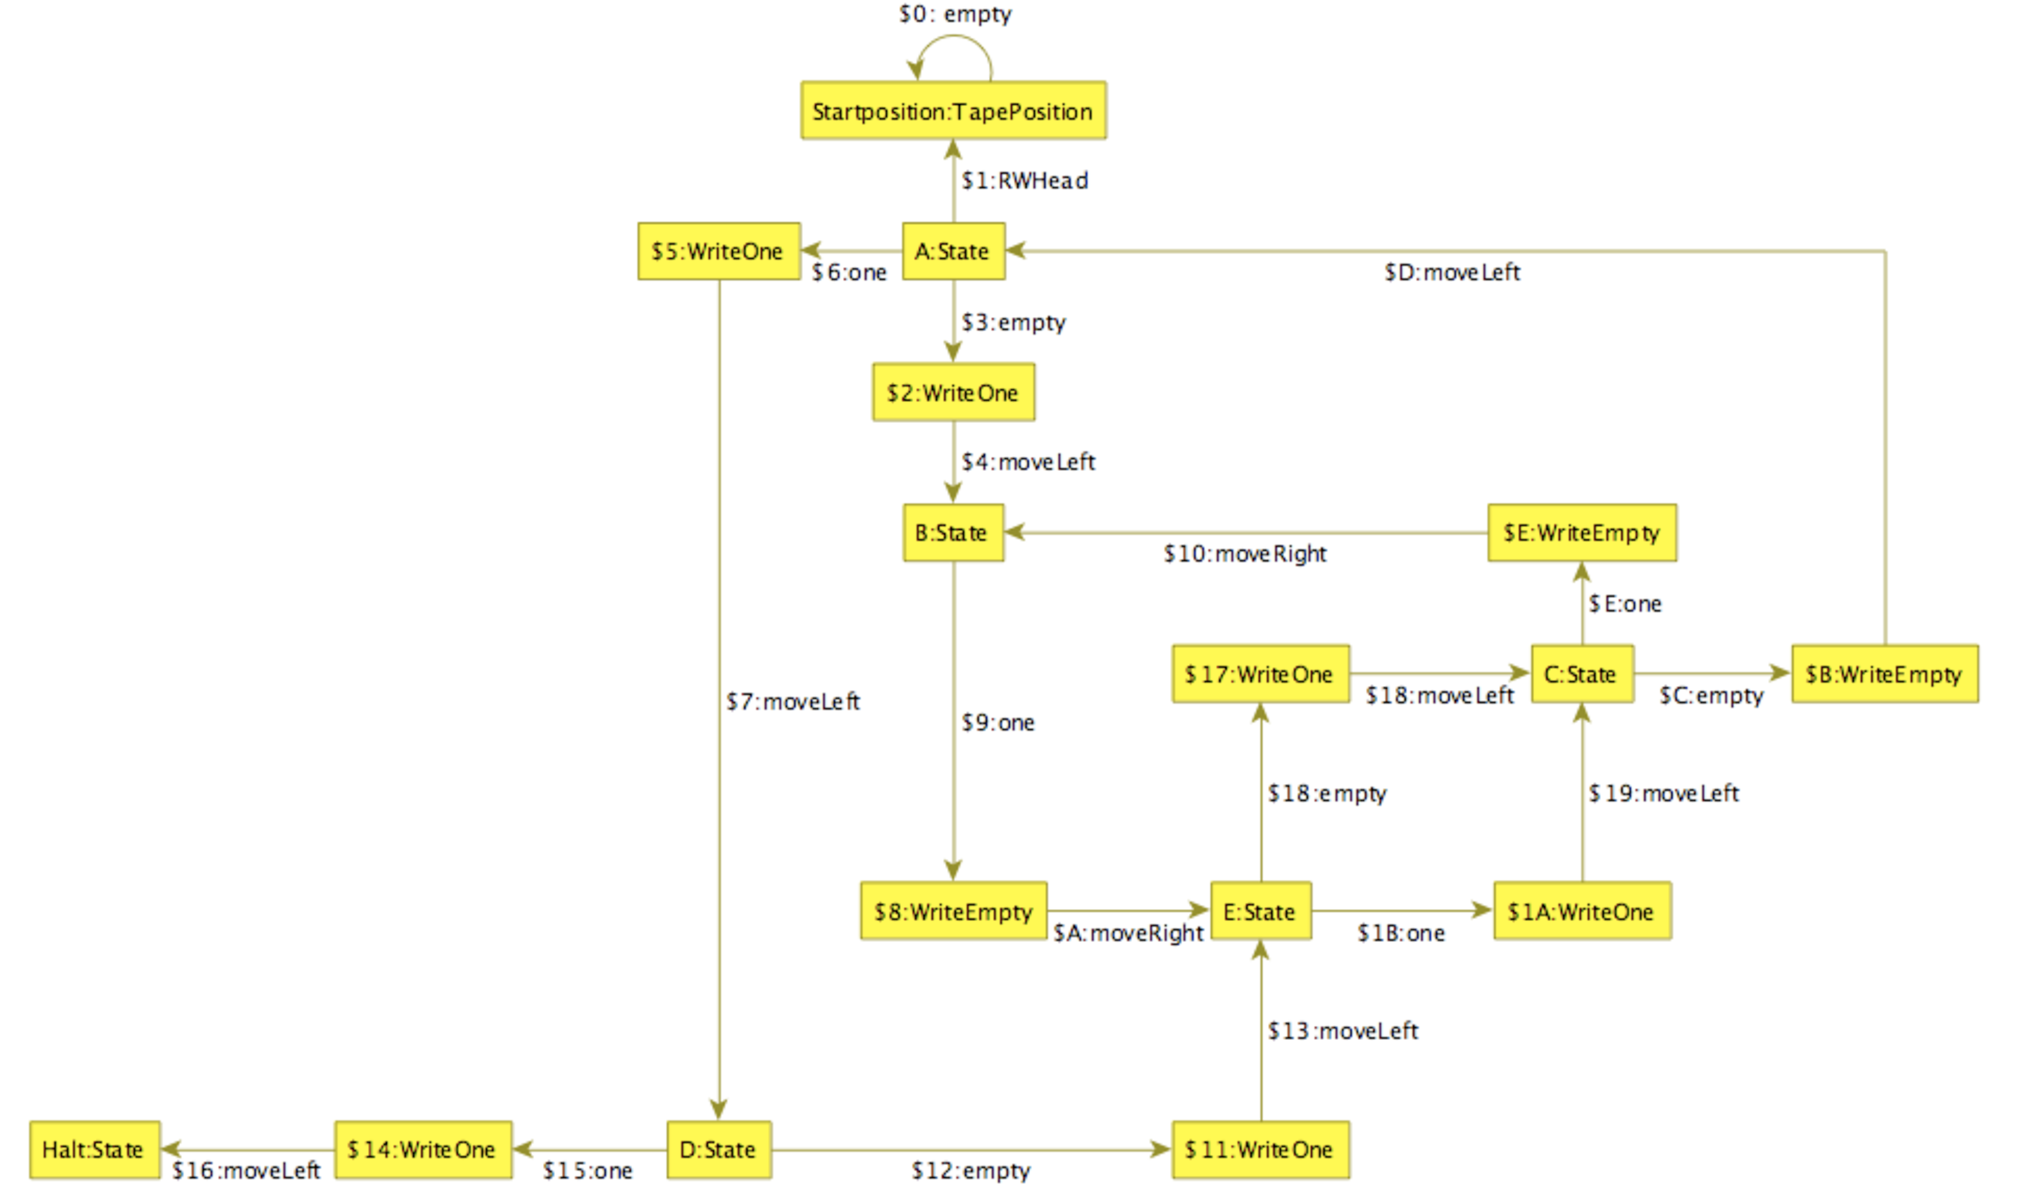
\includegraphics[width=\linewidth-2\fboxsep-2\fboxrule]{fig/bbstart}}
\end{center}

We have an initial host graph now. The graph rewrite sequence is quite straight forward and generic to the Turing graph model. Note that for each state the ``\texttt{\dots Empty\dots} | \texttt{\dots One\dots}'' selection is unambiguous.
%\pagebreak %HACK
\begin{grshell}[firstnumber=last]
  xgrs ((readOneRule | readEmptyRule) & (writeOneRule | writeEmptyRule) & (ensureMoveLeftValidRule | ensureMoveRightValidRule) & (moveLeftRule | moveRightRule))[32]

\end{grshell}
\quad\\We interrupt the machine after 32 iterations and look at the result so far:
\begin{center}
  \fbox{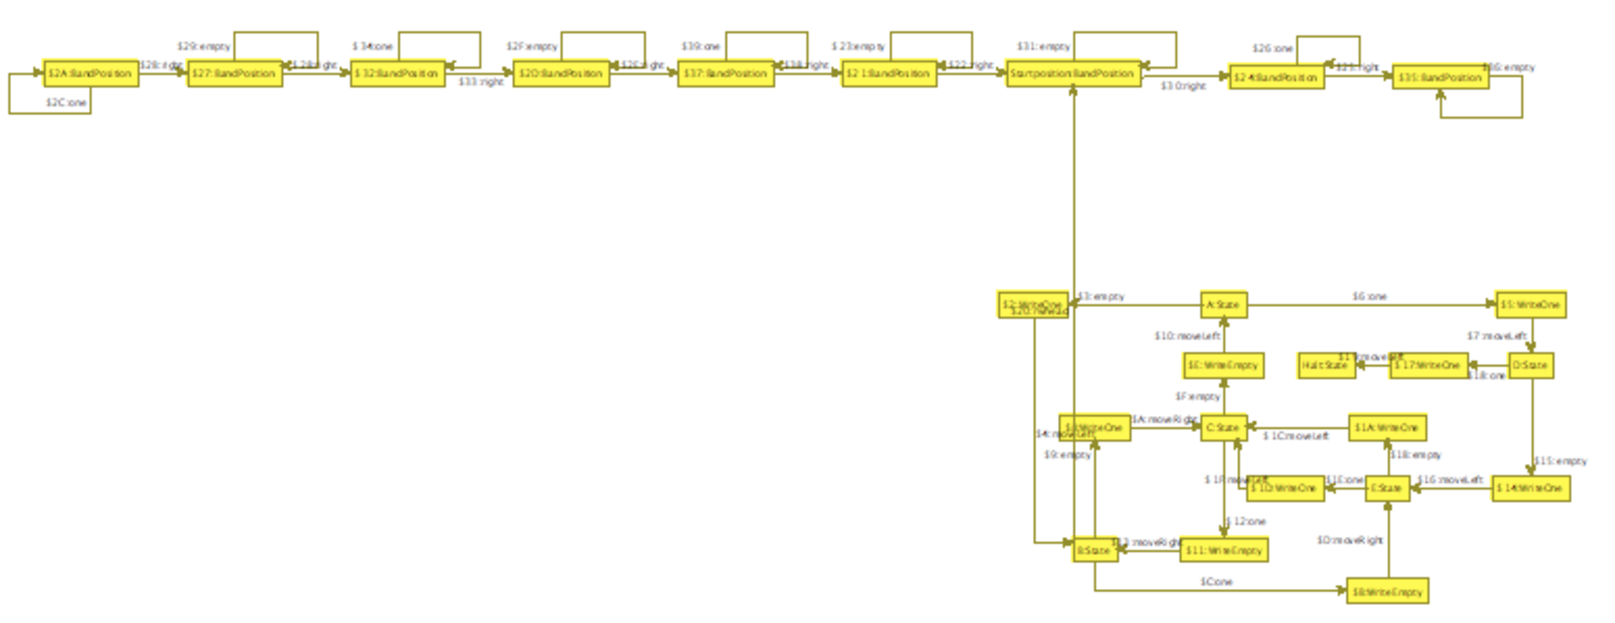
\includegraphics[width=\linewidth-2\fboxsep-2\fboxrule]{fig/bbmiddle}}
\end{center}
In order to improve the performance we generate better \indexed{search plan}s. This is a crucial step for execution time: With the initial search plans the beaver runs for 1 minute and 30 seconds. With improved search plans after the first 32 steps he takes about 8.5 seconds\footnote{On a Pentium 4, 3.2Ghz, with 2GiB RAM.}.
\begin{grshell}[firstnumber=last]
custom graph analyze_graph
custom actions gen_searchplan readOneRule readEmptyRule writeOneRule writeEmptyRule ensureMoveLeftValidRule ensureMoveRightValidRule moveLeftRule moveRightRule

\end{grshell}

Let the beaver run:
\begin{grshell}[firstnumber=last]
  xgrs ((readOneRule | readEmptyRule) & (writeOneRule | writeEmptyRule) & (ensureMoveLeftValidRule | ensureMoveRightValidRule) & (moveLeftRule | moveRightRule))*
\end{grshell}




\chapter{Application Programming Interface}\indexmainsee{application programming interface}{API} \indexmain{API}
\label{cha:api}

This chapter describes the Application Programming Interface of \GrG, i.e. of the system runtime - the LibGr - and of the assemblies generated from the model and rule specifications.
We'll have a look at
\begin{itemize}
\item the interface to the graph and model
\item the interface to the rules and matches
\item the interface of the graph processing environment
\item the porter module for importing and exporting of graphs and miscellaneous stuff
\item implementing external class and function declarations
\item implementing external match filter and external sequence declarations
\item events fired when the graph is changed
\item events fired during action execution
\end{itemize}

\noindent From the input file \texttt{Foo.grg} \texttt{grgen.exe} generates the output files \texttt{FooModel.cs} for the model and \texttt{FooActions.cs} for the actions,
\begin{itemize}
\item defining the exact interface, 
\item implementing the exact interface with generated code and code from the lgsp backend, i.e. entities from \texttt{de.unika.ipd.grGen.lgsp} available from lgspBackend.dll, 
\item and implementing the generic interface from \texttt{de.unika.ipd.grGen.libGr} using the entities mentioned in both points above.
\end{itemize}

\noindent This generative approach bears a great deal of the responsibility for the high execution speed of GrGen.NET, but it comes at the price of flexibility: you can't extend the rule set at runtime with new rules.
What you can do at runtime on the other hand is to generate a new rule set file, apply the compiler, and dynamically link the resulting assemblies/dlls.

When working with the API, you could reference the generated binary dlls in your project, in the same way as you have to reference the \texttt{libGr.dll} and \texttt{lgspBackend.dll}.
For easier debugging though, especially when you are integrating the generated code with own extensions (as described in chapter \ref{chapextensions}), it is recommended to directly include the source code generated (which is thrown away normally after it was compiled into the assemblies lgsp-FooModel.dll and lgsp-FooActions.dll).
For this, use the \texttt{-keep} option when you call \texttt{grgen.exe}, and include the model and the actions file (excluding the intermediate actions file) directly as C\# source code files.

The matcher code generated contains the initial, static search plans.
When you analyze the graph at runtime and generate new matchers, see section \ref{custom} for more on this, you can request the dumping of the source code of the improved matchers.
The custom commands are available at API level via the \texttt{Custom} operation of the \texttt{IGraph} interface for the graph commands and the \texttt{Custom} operation of the \texttt{BaseActions} class for the actions commands, just handing in the same parameters as otherwise specified on the command line.
If the intended workflow of ``i) loading a typical graph or doing a warm-up run creating a typical graph, ii) analyzing that graph, iii) compiling new matchers which are better suited to the graph'' is not easily achievable, or you want to start with the optimized matchers straight from the beginning, you may copy and paste the dumped dynamic matchers of an example run to the existing static code. 
But this is only a last resort, as the price is that your manual editing is overwritten again with the static search plans at the next time you call \texttt{grgen}.


%%%%%%%%%%%%%%%%%%%%%%%%%%%%%%%%%%%%%%%%%%%%%%%%%%%%%%%%%%%%%%%%%%%%%%%%%%%%%%%%%%%%%%%%%%%%%%%%
\section{Interface to the Host Graph}

The generated file \texttt{FooModel.cs} opens the namespace \texttt{de.unika.ipd.grGen.Model\_Foo} containing all the generated entities.
It contains for every node or edge class \texttt{Bar} an interface \texttt{IBar}, which offers C\# properties giving access to the attributes, and is inheriting in the same way as specified in the model file.
This builds the exact interface of the model, it is implemented by a sealed class \texttt{Bar} with generated code and with code from the lgsp backend.
Furtheron the namespace contains a model class \texttt{FooGraphModel} implementing the interface \texttt{de.unika.ipd.grGen.libGr.IGraphModel},
which supports iteration over the entities defined in the model using further, generic(i.e. inexact) interfaces from libGr.
Finally, the namespace contains a class \texttt{FooGraph} which defines an \texttt{LGSPGraph} of a model equivalent to \texttt{FooGraphModel}; 
it contains convenience functions to easily create nodes and edges of exact type in the graph.
In addition, a class \texttt{FooNamedGraph} is available, which defines an \texttt{LGSPNamedGraph} of a model equivalent to \texttt{FooGraphModel}; 
the named graph offers persistent names \ref{persistentex} for all its graph elements, otherwise it is identical to an \texttt{LGSPGraph}.
The naming requires about the same memory as an unnamed graph, but under normal circumstances the named graph is the recommended one to use (and is the one which will be used if employed by the shell).

\begin{note}
If you want to use the type-safe interface, use the interface \texttt{IBar}, and the \texttt{CreateNodeBar}-methods of \texttt{FooGraph} or the \texttt{CreateNode}-method of \texttt{Bar}.
If you want to use the generic interface, your entry point is the \texttt{IGraphModel}, with \texttt{INodeModel.GetType("Bar")} returning a \texttt{NodeType}, used in \texttt{IGraph.AddNode(NodeType)} returning an \texttt{INode}.
\end{note}


%%%%%%%%%%%%%%%%%%%%%%%%%%%%%%%%%%%%%%%%%%%%%%%%%%%%%%%%%%%%%%%%%%%%%%%%%%%%%%%%%%%%%%%%%%%%%%%%
\section{Interface to the Rules}

The generated file \texttt{FooActions.cs} opens the \texttt{namespace de.unika.ipd.grGen.Action\_Foo} containing all the generated entities.
It contains for every rule or test \texttt{bar}
\begin{itemize}
\item a class \texttt{Rule\_bar} inheriting from \texttt{de.unika.ipd.grGen.lgsp.LGSPRulePattern}, which contains
the exact match interface \texttt{IMatch\_bar} which defines how a match of the rule looks like,
extending the generic rule-unspecific \texttt{IMatch} interface.
Have a look at section \ref{sub:extflt} for an extended introduction to the matches interfaces. 
Furtheron there are (but meant only for internal use): a match class \texttt{Match\_bar} implementing the exact and inexact interface,
a description of the pattern to match, and the modify methods doing the rewriting.
\item an exact action interface \texttt{IAction\_bar} which contains the methods:
  \begin{itemize}
  \item \texttt{Match}, to match the pattern in the host graph,
     with in-parameters corresponding to the in-parameters of the rule (name and type),
	 returning matches of the exact type \texttt{Rule\_bar.IMatch\_bar}.
  \item \texttt{Modify}, to modify a given match according to the rewrite specification,
     with out-parameters corresponding to the out-parameters of the rule.
  \item \texttt{Apply}, to match and modify the found match,
     with in-parameters corresponding to the in-parameters of the rule,
     and with ref-parameters corresponding to the out-parameters of the rule.
  \end{itemize}
  Furtheron there is (but meant only for internal use) the class \texttt{Action\_bar} implementing the exact action interface as well as the generic \texttt{IAction} interface from libGr;
  it contains the generated matcher code searching for the patterns.
\end{itemize}

Moreover the namespace contains an action class \texttt{FooActions}
implementing the abstract class \texttt{de.unika.ipd.grGen.libGr.BaseActions} (in fact \texttt{de.unika.ipd.grGen.lgsp.LGSPActions}),
which supports iteration over the entities defined in the actions using further, generic(i.e. inexact) interfaces from libGr.
Additionally, at runtime it contains the instances of the actions singletons,
as member \texttt{bar} of the exact type \texttt{IAction\_bar}.
\begin{note}
If you want to use the type-safe interface, your entry point is the member \texttt{bar} of type \texttt{IAction\_bar} from \texttt{FooActions} (or \texttt{Action\_bar.Instance}).
Actions are used with named parameters of exact types.
If you want to use the generic interface, your entry point is the method \texttt{GetAction("bar")} of the interface \texttt{BaseActions} implemented by \texttt{FooActions} returning an \texttt{IAction}.
Actions are used with \texttt{object}-arrays for parameter passing.
\end{note}

\begin{note}
The old generic interface of string names and entities of node-,edge-, and object-type is implemented with the new interface of exactly typed, named entities.
Thus you will receive runtime exceptions when doing operations which are not type-safe with the generic interface, in contrast to \GrG\ $<$ v2.5.
If you need the flexibility of the old input parameters semantics of silently failing rule application on a wrong type,
you must declare it explicitly with the syntax \verb#r(x:ExactType<InexactType>)#;
then the rule parameter in the exact interface will be of type \texttt{InexactType}.
\end{note}

\begin{example}\label{ex:api1}
Normally you want to use the type-safe interface of the generated code as it is much more convenient.
Only if your application must get along with models and actions unknown before it is compiled you have to fall back to the generic interface.
An extensive example showing how to cope with the latter is shipped with \GrG\ in form of the GrShell.
Here we'll show a short example on how to use \GrG\ with the type-safe API; 
further examples are given in the examples-api folder of the \GrG-distribution.

We'll start with including the namespaces of the libGr and the lgsp backend shipped with \GrG\,
plus the namespaces of our actions and models, generated from \texttt{Foo.grg}.
\begin{verbatim}
using de.unika.ipd.grGen.libGr;
using de.unika.ipd.grGen.lgsp;
using de.unika.ipd.grGen.Action_Foo;
using de.unika.ipd.grGen.Model_Foo;
\end{verbatim}

Then we create a graph with model bound at generation time and create actions to operate on this graph.
Afterwards we create a single node of type \texttt{Bar} in the graph and save it to the variable \texttt{b}.
Finally we apply the action \texttt{bar(Bar x) : (Bar)} to the graph with \texttt{b} as input receiving the output as well.
The rule is taken from the actions via the member named as the action.
\begin{verbatim}
FooGraph graph = new FooGraph();
FooActions actions = new FooActions(graph);
Bar b = graph.CreateNodeBar();
actions.bar.Apply(graph, b, ref b); // input of type Bar, output of type Bar
\end{verbatim}

We could create a named graph instead offering persistent names for its graph elements:
\begin{verbatim}
FooNamedGraph graph = new FooNamedGraph();
\end{verbatim}
\end{example}

\begin{example}
This is an example doing mostly the same as the previous example \ref{ex:api1}, in a slightly more complicated way allowing for more control.
Here we create the model separate from the graph, then the graph with a model not bound at generation time.
We create the actions to apply on the graph, and a single node of type \texttt{Bar} in the graph, which we assign again to a variable \texttt{b}.
Then we get the action from the actions and save it to an action variable \texttt{bar};
afterwards we use the action for finding all available matches of \texttt{bar} with input \texttt{b} -- which is different from the first version -- and remember the found matches in the matches variable with its exact type.
Finally we take the first match from the matches and execute the rewrite with it.
We could have inspected the nodes and edges of the match or their attributes before (using element names prefixed with \texttt{node\_/edge\_} or attribute names to get exactly typed entities). 
\begin{verbatim}
IGraphModel model = new FooGraphModel();
LGSPGraph graph = new LGSPGraph(model);
FooActions actions = new FooActions(graph);
Bar b = Bar.CreateNode(graph);
IAction_bar bar = Action_bar.Instance;
IMatchesExact<Rule_bar.IMatch_bar> matches = bar.Match(graph, 0, b);
bar.Modify(graph, matches.First);
\end{verbatim}

We could create a named graph instead offering persistent names for its graph elements:
\begin{verbatim}
LGSPGraph graph = new LGSPNamedGraph(model);
\end{verbatim}
\end{example}

%%%%%%%%%%%%%%%%%%%%%%%%%%%%%%%%%%%%%%%%%%%%%%%%%%%%%%%%%%%%%%%%%%%%%%%%%%%%%%%%%%%%%%%%%%%%%%%%
\section{Interface of the Graph Processing Environment}

The interface \texttt{IGraphProcessingEnvironment} implemented by the \texttt{LGSPGraphProcessing\-Environment} class offers all the additional functionality of \GrG~exceeding what is offered by the graph and the actions.
It is constructed as \texttt{LGSPGraphProcessingEnvironment} given the graph and the actions.
It offers execution of the sequences and variable handling, combining actions into transformations
(the former regarding control flow, the latter regarding data flow).

\begin{example}\label{ex:procenv}
For all but the simplest transformations you'll end up constructing a graph processing environment from the graph and the actions constructed until now, executing a graph rewrite sequence on the graph processing environment:
\begin{verbatim}
LGSPGraphProcessingEnvironment procEnv = 
    new LGSPGraphProcessingEnvironment(graph, actions);
procEnv.ApplyGraphRewriteSequence("<(::x)=foo && (::y)=bar(::x) | bla(::y)>");
\end{verbatim}
\end{example}

In addition to sequences and variables handling, the graph processing environment offers driver or helper objects for transaction management, deferred sequence execution, graph change recording, and emitting.
The most important of these is the transaction manager which is utilized when \GrG~ is used for crawling through a search space or for enumerating a state space, see section \ref{sec:extctrl}.
The operations mentioned there are implemented by calling the function given in example \ref{ex:transman}.

\begin{example}\label{ex:transman}
\begin{verbatim}
LGSPGraphProcessingEnvironment procEnv = ...;
ITransactionManager tm = procEnv.TransactionManager;
public interface ITransactionManager
{
    int Start();
    void Pause();
    void Resume();
    void Commit(int transactionID);
    void Rollback(int transactionID);
}
\end{verbatim}
\end{example}

The \texttt{Start} starts a transaction and returns its id; it may be called multiple times returning different ids for the then nested transactions (i.e. a failing outer one rolls back the changes of an inner transaction which succeeded).
Changes to the graph are recorded thereafter into an undo log, unless a \texttt{Pause} was called not yet followed by a \texttt{Resume}.
When the changes of interest were carried out the transaction identified by its id is either \texttt{Commit}ed, which causes the changes recorded since the corresponding \texttt{Start} to stay in the graph, or rolled back by calling \texttt{Rollback}, in that case all the changes recorded since the corresponding \texttt{Start} are undone.

%%%%%%%%%%%%%%%%%%%%%%%%%%%%%%%%%%%%%%%%%%%%%%%%%%%%%%%%%%%%%%%%%%%%%%%%%%%%%%%%%%%%%%%%%%%%%%%%
\section{Import/Export and Miscellaneous Stuff}\label{sub:imexport}\indexmain{import}\indexmain{export}

GrGen natively supports the following formats:
\begin{description}
  \item[GRS/GRSI] Reduced GrShell script files (graph only, model from \texttt{.gm}; a very limited version of the normal \texttt{.grs}. The recommended standard format.)
  \item[GXL] Graph eXchange Language (\texttt{.gxl}-files, see \url{http://www.gupro.de/GXL/})
  \item[ECORE/XMI] Ecore(\texttt{.ecore}) model files and XMI(\texttt{.xmi}) graph file. Import only, export must be programmed with \texttt{emit}-statements. In an intermediate step, a \texttt{.gm} file is generated for the model.
    \item[GRG] Writes a GrGen rule file containing one rule with an empty pattern and a large rewrite part. Export only \footnote{Original German Pisswasser, for export only :)}, not for normal use.
\end{description}

While both GRS and GXL importers expect one file
(the GXL importer allows to specify a model override, see GrShell import, Note \ref{shellgxlimport}),
the EMF/ECORE importer expects first one or more \texttt{.ecore} files
and following optionally a \texttt{.xmi} files and/or a \texttt{.grg} file (cf. Note \ref{shellecoreexport}). 
To use additional custom graph models you should supply an own \texttt{.grg}
file which may be based on the automatically generated \texttt{.grg} file, if none was
supplied (see the Program-Comprehension example in \texttt{examples/ProgramComprehension-GraBaTs09}).

To import a graph model and/or a graph instance you can use \texttt{Porter.Import()} from the libGr API (the GrShell command \texttt{import} is mapped to it)
The file format is determined by the file extensions.
To export a graph instance you can use \texttt{Porter.Export()} from the libGr API (the GrShell command \texttt{export} is mapped to it).
For an example of how to use the importer/exporter on API level see \texttt{examples-api/JavaProgramGraphsExample/JavaProgramGraphs\-Example.cs}

The GRS(I) importer returns an \texttt{INamedGraph};
if you don't need the persistent names, get rid of them by casting to the \texttt{LGSPNamedGraph} implementing the interface, (copy-)constructing a \texttt{LGSPGraph} from it, and forgetting any references to the named graph.
Please be aware that naming is rather expensive:
A \texttt{LGSPNamedGraph} supplying the name to element and element to name mappings normally uses up about twice the amount of memory of the \texttt{LGSPGraph} defining the graph alone (but is worth is most often).

\subsection*{External Emitting and Parsing}\label{sub:apiextemitparse}
If \texttt{emit class;} (see \ref{sub:extemitparse}) is specified in the model file \texttt{Foo}, \GrG~generates a file \texttt{FooModelExternalFunctions.cs} located besides the model and rule files,
containing the following functions.

\begin{csharplet}
/// <summary>
/// Called during .grs import, at exactly the position in the text reader where the attribute begins.
/// For attribute type object or a user defined type, which is treated as object.
/// The implementation must parse from there on the attribute type requested.
/// It must not parse beyond the serialized representation of the attribute, 
/// i.e. Peek() must return the first character not belonging to the attribute type any more.
/// Returns the parsed object.
/// </summary>
object Parse(TextReader reader, AttributeType attrType, IGraph graph);

/// <summary>
/// Called during .grs export, the implementation must return a string representation for the attribute.
/// For attribute type object or a user defined type, which is treated as object.
/// The serialized string must be parseable by Parse.
/// </summary>
string Serialize(object attribute, AttributeType attrType, IGraph graph);

/// <summary>
/// Called during debugging or emit writing, the implementation must return a string representation for the attribute.
/// For attribute type object or a user defined type, which is treated as object.
/// The attribute type may be null.
/// The string is meant for consumption by humans, it does not need to be parseable.
/// </summary>
string Emit(object attribute, AttributeType attrType, IGraph graph);
\end{csharplet}

\texttt{Parse} is called when an attribute of an external or object type is to be imported from a grs file, \texttt{Serialize} is called when an attribute of an external or object type is to be exported to a grs file, and \texttt{Emit} is called when a value of external or object type is to be emitted, or displayed in the debugger, including yComp.
(The functions are called from GrShell, too, insofar as possible -- the shell parses a single or double quoted text or a word or a number at an attribute position and hands that over then to the user defined parser.)
They forward the calls to \texttt{ParseImpl}, \texttt{SerializeImpl}, and \texttt{EmitImpl} functions, that need to be implemented in a file named \texttt{FooModelExternal\-FunctionsImpl.cs} located in the folder of the \texttt{FooModelExternalFunctions.cs} file.
Implementing them is \emph{your} task, in exchange you get a tight integration of your own datatypes into \GrG.
You may have a look at \texttt{tests/ExternalAttributeEvaluation} or  \texttt{examples\-api/ExternalAttributeEvaluationExample} for an example.


\subsection*{External Copying and Comparing}\label{sub:apiextcopycompare}
If \texttt{copy class;} or \texttt{== class;} or \texttt{< class;} (see \ref{sub:extcopycompare}) are specified in the model file \texttt{Foo},
\GrG~generates a file \texttt{FooModelExternalFunctions.cs} located besides the model and rule files,
containing a partial class \texttt{AttributeTypeObjectCopierComparer} expecting that the \texttt{Copy} or the \texttt{IsEqual} or the \texttt{IsLower} functions are implemented in the same partial class in \texttt{FooModelExternalFunctionsImpl.cs}.
For every external type defined a further pair of functions with that type used in the input parameters is expected.

\begin{csharplet}
// Called when a graph element is cloned/copied.
// For attribute type object.
// If "copy class" is not specified, objects are copied by copying the reference, i.e. they are identical afterwards.
// All other attribute types are copied by-value (so changing one later on has no effect on the other).
public static object Copy(object);

// Called during comparison of graph elements from graph isomorphy comparison, or attribute comparison.
// For attribute type object.
// If "== class" is not specified, objects are equal if they are identical,
// i.e. by-reference-equality (same pointer); all other attribute types are compared by-value.
public static bool IsEqual(object, object);

// Called during attribute comparison.
// For attribute type object.
// If "< class" is not specified, objects can't be compared for ordering, only for equality.
public static bool IsLower(object, object);
\end{csharplet}

\texttt{Copy} is called when one of the copy operations offered in the rule language or the computation statements is executed on a node or edge that bears attributes of object or user defined type.
\texttt{IsEqual} is called when two graphs are compared for isomorphy and the graph elements contain attributes of object or user-defined external types, or if attributes of object or user defined type are compared with one of the equality operators.
\texttt{IsLower} is called when attributes of object or user defined type are compared with one of the relational operators.
A comparison for \texttt{u<=v} is mapped to an expression \verb#IsLower(u,v) || IsEqual(u,v)#, this is why a \verb#< class;# specification requires a preceding \verb#== class;# specification.

Implementing those functions is \emph{your} task, in exchange you get a tight integration of your own datatypes into \GrG.
You may have a look at \texttt{tests/ExternalAttributeEvaluation} or  \texttt{examples\-api/ExternalAttributeEvaluationExample} for an example.

\subsection*{Further Examples}
There are further examples available in the \texttt{examples-api} folder of the \GrG-distribution:
\begin{itemize} 
\item How to use the graph rewrite sequences offered by the libGr on API level is shown in\\
\texttt{examples-api/BusyBeaverExample/BusyBeaverExample.cs}.\\
But normally you want to use your favourite .NET programming language for control together with the type-safe interface when working on API level.
\item How to use the old and new interface for accessing a match on API level is shown in\\
\texttt{examples-api/ProgramGraphsExample/ProgramGraphsExample.cs}.
\item How to use the visited\label{apiallocvisitflag} flags on API level is shown in\\
\texttt{examples-api/VisitedExample/VisitedExample.cs}.
\item How to analyze the graph and generate (hopefully) better performing matchers based on this information is shown in\\
\texttt{examples-api/BusyBeaverExample/BusyBeaverExample.cs}.
\item How to compile a \texttt{.grg}-specification at runtime and dump a graph for visualization in \texttt{.vcg} format on the API level is shown in\\
\texttt{examples-api/HelloMutex/HelloMutex.cs}.
\item How to access the annotations at API level is shown in\\
\texttt{examples-api/MutexDirectExample/MutexDirectExample.cs}.
\item How to communicate with yComp on the API level (from your own code) is shown in\\
\texttt{examples-api/YCompExample/YCompExample.cs} (it may be outdated, you better take a look at \texttt{GrShell/YCompClient.cs} for the real version).
\end{itemize}

\begin{warning}
While C\# allows input arguments values to be of a subtype of the declared interface parameter type (OO), 
it requires that the argument variables for the \texttt{out} parameters are of exactly the type declared (non-OO).
Although a variable of a supertype would be fully sufficient -- the variable is only assigned.
So for \texttt{node class Bla extends Bar;} and action \texttt{bar(Bar x) : (Bla)} from the rules file rules \texttt{Foo.grg}
we can't use a desired target variable of type \texttt{Bar} as \texttt{out}-argument,
but are forced to introduce a temporary variable of type \texttt{Bla}
and assign this variable to the desired target variable after the call.
\begin{csharplet}
using de.unika.ipd.grGen.libGr;
using de.unika.ipd.grGen.lgsp;
using de.unika.ipd.grGen.Action_Foo;
using de.unika.ipd.grGen.Model_Foo;
FooGraph graph = new FooGraph();
FooActions actions = new FooActions(graph);
Bar b = graph.CreateNodeBar();
IMatchesExact<Rule_bar.IMatch_bar> matches = actions.bar.Match(graph, 1, b);
//actions.bar.Modify(graph, matches.First, out b); // wont work, needed:
Bla bla = null; 
actions.bar.Modify(graph, matches.First, out bla);
b = bla;
\end{csharplet}
\end{warning}


%%%%%%%%%%%%%%%%%%%%%%%%%%%%%%%%%%%%%%%%%%%%%%%%%%%%%%%%%%%%%%%%%%%%%%%%%%%%%%%%%%%%%%%%%%%%%%%%
\section{External Class, Function and Procedure Implementation}\label{sub:extclsfctimpl}\indexmain{external class implementation}\indexmain{external function implementation}\indexmain{external procedure implementation}

For a model file \texttt{Foo} which contains external functions (cf. \ref{sub:extfct}) and/or classes (cf. \ref{sub:extcls}), \GrG~generates a file \texttt{FooModelExternalFunctions.cs} located besides the model and rule files, which contains
\begin{itemize}
	\item within the model namespace public partial classes named as given in the external class declaration,
inheriting from each other as stated in the external class declarations.
	\item within the \texttt{de.unika.ipd.grGen.expression} namespace a public partial class named \texttt{ExternalFunctions} with a body of comments giving the expected function and procedure prototypes.
\end{itemize}

\noindent The partial classes are empty, you must implement them in a file named \texttt{FooModelExternal\-FunctionsImpl.cs} located in the folder of the \texttt{FooModelExternalFunctions.cs} file by
\begin{itemize}
	\item fleshing out the partial classes skeletons with attributes containing data of interest and maybe helper methods
	\item fleshing out the \texttt{ExternalFunctions} partial class skeleton with the functions you declared in the external function declarations, obeying the function signatures as specified; here you can access the now know attributes or methods of the external classes, or do complicated custom computations or graph querying with the values you receive from a function call.
	\item fleshing out the \texttt{ExternalProcedures} partial class skeleton with the procedures you declared in the external procedure declarations, obeying the procedure signatures as specified; here you can access the now know attributes or methods of the external classes, or do complicated custom computations or graph manipulations with the values you receive from a procedure call.
\end{itemize}

\noindent Don't forget that the source code file \texttt{FooModelExternalFunctionsImpl.cs} is an integral part of your \GrG~graph transformation project, in contrast to the other C\# files generated (and overwritten) for you.
In \texttt{examples/ExternalAttributeEvaluationExample} and \texttt{examples-api/ExternalAttributeEvaluationExample}
you find a fabricated example showing how to use the external classes and functions.

When you use third-party assemblies in your source code you must inform GrGen.NET about them so references to them are included into the assembly generated; this can be done with the \texttt{-r} parameter when calling \texttt{grgen.exe} directly (cf. \ref{grgenoptions}) or with the \texttt{new} command configurations available in GrShell (cf. \ref{graphcommands}). Using the \texttt{keepdebug} configuration of the \texttt{new} command is recommended as it allows for easier debugging.


%%%%%%%%%%%%%%%%%%%%%%%%%%%%%%%%%%%%%%%%%%%%%%%%%%%%%%%%%%%%%%%%%%%%%%%%%%%%%%%%%%%%%%%%%%%%%%%%
\section{External Filter and Sequence Implementation}\label{sub:extfltseqimpl}\indexmain{external match filter implementation}\indexmain{external sequence implementation}

For an actions file \texttt{Bar} which contains match filter declarations (cf. \ref{sub:extflt}) and/or external sequence declarations (\ref{sub:extseq}), \GrG~generates a file \texttt{BarActionsExternalFunctions.cs} located besides the model and rule files, which contains within the action namespace 
\begin{itemize}
	\item a public partial class named \texttt{MatchFilters} with a body of comments giving the expected function prototypes, and for the \texttt{auto} filters even the implementation.
	\item public partial classes, named \texttt{Sequence\_foo} for a sequence \texttt{foo}, with a body containing a comment specifying the expected function prototype of the sequence application function.
\end{itemize}

\noindent The partial classes are empty, you must implement them in a file named \texttt{BarActionsExternal\-FunctionsImpl.cs} located in the folder of the \texttt{BarActionsExternalFunctions.cs} file by
\begin{itemize}
	\item fleshing out the \texttt{MatchFilters} partial class skeleton with the match filter functions you declared, obeying the function signatures as specified; you might want to convert the received matches object to an \texttt{IList} in case you want to reorder the list and reinject it into the matches object afterwards.
	\item fleshing out the partial classes skeletons of the external sequence with the \texttt{ApplyXGRS\_foo} methods needed.
\end{itemize}

\noindent Don't forget that the source code file \texttt{BarActionsExternalFunctionsImpl.cs} is an integral part of your \GrG~graph transformation project, in contrast to the other C\# files generated (and overwritten) for you.
In \texttt{examples/ExternalFiltersAndSequencesExample} and \texttt{examples-api/ExternalFiltersAndSequencesExample}
you find a fabricated example showing how to use the external classes and functions.

When you use third-party assemblies in your source code you must inform GrGen.NET about them so references to them are included into the assembly generated; this can be done with the \texttt{-r} parameter when calling \texttt{grgen.exe} directly (cf. \ref{grgenoptions}) or with the \texttt{new} command configurations available in GrShell (cf. \ref{graphcommands}). Using the \texttt{keepdebug} configuration of the \texttt{new} command is recommended as it allows for easier debugging.

\begin{note}\label{note:inspect}
\LibGr\ allows for splitting a rule application into two steps:
Find all the subgraphs of the host graph that match the pattern first, then rewrite one of these matches. 
By returning a collection of all matches, the \LibGr\ retains the complete graph rewrite process under control.
As a \LibGr\ user have a look at the following methods of the \texttt{IAction} interface:
\begin{csharplet}
IMatches Match(IGraph graph, int maxMatches, object[] parameters);
object[] Modify(IGraph graph, IMatch match);
\end{csharplet}

In C\#, this might look like:
\begin{csharplet}
IMatches myMatches = myAction.Match(myGraph, -1, null); /* -1: get all the matches */
for(int i=0; i<myMatches.NumMatches; ++i)
{
	if(inspectCarefully(myMatches.GetMatch(i))
	{
		myAction.Modify(myGraph, myMatches.GetMatch(i));
		break;
  	}
}
\end{csharplet}

The external match filters are hooking in between the \texttt{Match} and \texttt{Modify} functions, they allow you to do this kind of inspection without being forced to resort to fully external control.
The most interesting filter can be automatically generated for you, the \texttt{auto} filter for filtering symmetric matches of automorphic patterns, see \ref{sub:extflt} for more on this.
\end{note}


%%%%%%%%%%%%%%%%%%%%%%%%%%%%%%%%%%%%%%%%%%%%%%%%%%%%%%%%%%%%%%%%%%%%%%%%%%%%%%%%%%%%%%%%%%%%%%%%
\section{Graph Events}\label{sec:graphevent}

Before or after the host graph is changed, events are fired, notifying listeners about the changes.
The GrShell debugger, the transaction handler, and the graph change recorder implement their functionality by listening and reacting to these events.
A programmer may add own event handlers to insert custom-made, event-based functionality;
or may even implement an event-driven rule execution engine on top of it.
The events are fired automatically by the \texttt{LGSPGraph} implementing the \texttt{IGraph},
or by the rules which get applied.
If you operate on API level or with e.g. external sequences, it's your responsibility to fire the events for attribute changes before changing an attribute.
Otherwise the changes won't be visible in the debugger, they won't be rolled back at the end of a transactions or during backtracking, and they won't be recorded in case of change recording.
If you listen to or fire the rule application events (cf. \ref{sec:actionevent}), you may be interested in the added names event, too, which tells about the names of the elements which will get added immediately thereafter (this is used in the debugger to display the names of the elements as defined in the rule modify part).

The events available which are fired automatically are:
\begin{csharplet}
// Fired after a node has been added
event NodeAddedHandler OnNodeAdded;

// Fired after an edge has been added
event EdgeAddedHandler OnEdgeAdded;

// Fired before a node is deleted
event RemovingNodeHandler OnRemovingNode;

// Fired before an edge is deleted
event RemovingEdgeHandler OnRemovingEdge;

// Fired before all edges of a node are deleted
event RemovingEdgesHandler OnRemovingEdges;

// Fired before the whole graph is cleared
event ClearingGraphHandler OnClearingGraph;

// Fired before the type of a node is changed.
event RetypingNodeHandler OnRetypingNode;

// Fired before the type of an edge is changed.
event RetypingEdgeHandler OnRetypingEdge;

// Fired before an edge is redirected (causing removal then adding again).
event RedirectingEdgeHandler OnRedirectingEdge;
\end{csharplet}

The events available which are fired automatically by code generated by GrGen for the actions, but which need to be fired by you in case you change the graph and want e.g. an accurate debugger display.

\begin{csharplet}
// Fired before an attribute of a node is changed.
event ChangingNodeAttributeHandler OnChangingNodeAttribute;

// Fired before an attribute of an edge is changed.
event ChangingEdgeAttributeHandler OnChangingEdgeAttribute;

// Fires an OnChangingNodeAttribute event.
// To be called before changing an attribute of a node,
// with exact information about the change to occur.
void ChangingNodeAttribute(INode node, AttributeType attrType,
    AttributeChangeType changeType, Object newValue, Object keyValue);

// Fires an OnChangingEdgeAttribute event.
// To be called before changing an attribute of a node,
// with exact information about the change to occur.
void ChangingEdgeAttribute(IEdge edge, AttributeType attrType,
    AttributeChangeType changeType, Object newValue, Object keyValue);        

// Fired before each rewrite step (also rewrite steps of subpatterns) to indicate 
// the names of the nodes added in this rewrite step in order of addition.
event SettingAddedElementNamesHandler OnSettingAddedNodeNames;

// Fired before each rewrite step (also rewrite steps of subpatterns) to indicate 
// the names of the edges added in this rewrite step in order of addition.
event SettingAddedElementNamesHandler OnSettingAddedEdgeNames;
\end{csharplet}

The events available which are fired automatically on visited flag changes are:

\begin{csharplet}
/// Fired after a visited flag was allocated.
event VisitedAllocHandler OnVisitedAlloc;

/// Fired after a visited flag was freed.
event VisitedFreeHandler OnVisitedFree;

/// Fired before a visited flag is set.
event SettingVisitedHandler OnSettingVisited;
\end{csharplet}

%%%%%%%%%%%%%%%%%%%%%%%%%%%%%%%%%%%%%%%%%%%%%%%%%%%%%%%%%%%%%%%%%%%%%%%%%%%%%%%%%%%%%%%%%%%%%%%%
\section{Action Events}\label{sec:actionevent}

When actions are executed, events are fired, notifying listeners about the changes.
The GrShell debugger implements its functionality by listening and reacting to these events.
A programmer may add own event handlers to insert custom-made, event-based functionality.
The events are fired automatically by the code generated by GrGen for the rules or sequences.
If you operate on API level or with e.g. external sequences, it's your responsibility to fire the events in case you want to simulate rules or sequences.

The rule based events declared by the \texttt{IActionExecutionEnvironment} are:

\begin{csharplet}
// Fired after all requested matches of a rule have been matched.
event AfterMatchHandler OnMatched;

// Fired before the rewrite step of a rule, when at least one match has been found.
event BeforeFinishHandler OnFinishing;

// Fired before the next match is rewritten. It is not fired before rewriting the first match.
event RewriteNextMatchHandler OnRewritingNextMatch;

// Fired after the rewrite step of a rule.
// Note, that the given matches object may contain invalid entries,
// as parts of the match may have been deleted!
event AfterFinishHandler OnFinished;
\end{csharplet}

The sequence based events declared by the \texttt{IGraphProcessingEnvironment} extending the \texttt{IActionExecutionEnvironment} are:
         
\begin{csharplet}
// Fired when a sequence is entered.
event EnterSequenceHandler OnEntereringSequence;

// Fired when a sequence is left.
event ExitSequenceHandler OnExitingSequence;

// Fired when a sequence iteration is ended.
event EndOfIterationHandler OnEndOfIteration;
\end{csharplet}

A special kind of sequence based events are the graph change events, fired when processing enters a subgraph or leaves a subgraph (fired when the subgraph usage stack is altered):

\begin{csharplet}
/// Fired when graph processing (rule and sequence execution) is switched to a (sub)graph.
/// (Not fired when the main graph is replaced by another main graph, or initialized.)
event SwitchToSubgraphHandler OnSwitchingToSubgraph;

/// Fired when graph processing is returning back after a switch.
/// (To the main graph, or a subgraph previously switched to.)
event ReturnFromSubgraphHandler OnReturnedFromSubgraph;
\end{csharplet}


\chapter{Extensions}\indexmain{extensions}\label{chapextensions}

This chapter lists the ways you can customize \GrG~without \GrG-language constructs and
shows how to interact with the external world outside of \GrG.
The primary means available are: external attribute types, external functions, match filters, and external sequences; the secondary helpers available are annotations, command line parameters, and external shell commands.

%-----------------------------------------------------------------------------------------------
\section{External Attribute Types}\label{sub:extcls}
\begin{rail}
  ExternalClassDeclaration: 'class' IdentDecl (() | 'extends' (NodeType+',')) ';';
\end{rail}\ixnterm{ExternalClassDeclaration}\ixkeyw{class}\ixkeyw{extends}
Registers a new attribute type with \GrG. You may declare the base types of the type, but not give attributes. The attribute type must be implemented externally, see \ref{sub:extclsfctimpl}; for \GrG~the type is opaque, only external functions can do computations with it. You may extend \GrG~with external attribute types if the built-in attribute types (cf. \ref{sec:builtintypes}) are insufficient for your needs.

%-----------------------------------------------------------------------------------------------
\section{External Function Types}\label{sub:extfct}
\begin{rail}
  ExternalFunctionDeclaration: IdentDecl '(' ( () | (Type + ',') ) ')' ':' Type ';';
\end{rail}\ixnterm{ExternalFunctionDeclaration}
Registers an \indexed{external function} with \GrG~to be used in attribue computation.
An external function declaration specifies the expected input types and the output type. The function must be implemented externally, see \ref{sub:extclsfctimpl}.
An external function call (cf. \ref{sec:primexpr}) may receive and return values of the built-in (attribute) types as well as of the external attribute types; the real arguments on the call sites are type-checked against the declared signature following the subtyping hierarchy of the built-in as well as of the external attribute types.
You may extend \GrG~with external functions if the built-in attribute computation capabilities (cf. \ref{sub:expr}) are insufficient for your needs.

%-----------------------------------------------------------------------------------------------
\section{External Match Filters}\label{sub:extflt}

\begin{rail}
  MatchFilter: ( backslash (IdentDecl + ',') )?;
\end{rail}\ixnterm{MatchFilter}

Registers one or multiple \indexed{external match filter}s with \GrG~, for the rule the match filters are appended at, to be used from selected applications of that rule (cf. \emph{FilterIdent} in \ref{sec:ruleapplication}).
The \indexed{match filter} function must be implemented externally, see \ref{sub:extfltseqimpl}.
You may extend \GrG~with match filters if you need to inspect the matches found for a rule in order to decide which to apply (see note \ref{note:inspect}) or if you just need a post-match hook which informs you about the found matches.

\subsubsection*{Match object}

For a rule or subpattern \texttt{r} GrGen generates a match interface \texttt{IMatch\_r} extending the generic \texttt{IMatch} interface from the \texttt{libGr}.
The basic constituents, i.e. nodes, edges and variables are mapped directly to members of their name and type, containing the graph element matched or the value computed.
For alternatives nested inside the pattern a common base interface \texttt{IMatch\_r\_altName} is generated, plus for each alternative case an interface \texttt{IMatch\_r\_altName\_altCaseName}. When you walk the matches tree using the type exact interface (which is recommended), you must type switch on the match object in the alternative variable, to determine the case which was finally matched, and cast to its match type.
For iterateds nested inside the pattern, in the pattern match object an iterated variable of type \texttt{IMatchesExact<IMatch\_r\_iteratedName>} is created; the IMatchesExact allows you to iterate over the patterns finally found. 
A subpattern usage is mapped directly to a variable in the match object typed with the match interface of the subpattern.
The same holds for independent patterns; negative patterns do not appear in the match objects, for they prevent the matching and thus the building of a match object in the first place.

%-----------------------------------------------------------------------------------------------
\section{External Sequences}\label{sub:extseq}
\begin{rail}
  ExternalSequenceDeclaration: 
    'sequence' RewriteSequenceSignature ';';
\end{rail}\ixnterm{ExternalSequenceDeclaration}
Registers an \indexed{external sequence} similar to a defined sequence (cf. \ref{sec:sequencedefinition}) but in contrast to that it must or can be implemented outside in C\# code.
An external sequence declaration specifies the expected input types and the output types. The sequence must be implemented externally, see \ref{sub:extfltseqimpl}.
You may extend \GrG~with external sequences if you want to call into external code to interface with libraries from outside the domain of graph rewriting, or if the \GrG-languages are not well suited for parts of the task at hand.

%-----------------------------------------------------------------------------------------------
\section{Shell Commands}

\begin{rail}
  '!' CommandLine
\end{rail}\indexmain{\texttt{"!}}
\emph{CommandLine} is execute as-is by the shell of the operating system.

%-----------------------------------------------------------------------------------------------
\section{Shell and Compiler Parameters}

\noindent When executing the \GrG\ generator/compiler \texttt{GrGen.exe}, the follwing parameters are admissible:

\noindent \texttt{[mono] GrGen.exe } \texttt{[-keep [<dest-dir>]] [-debug]} \texttt{[-lazynic] [-noinline]} \texttt{[-r <assembly-path>]}

The assembly \emph{assembly-path} is linked as reference to the compilation result with the \texttt{-r} parameter.

These compiler parameters can be configured in the GrShell to be used, too:
\begin{rail}
  'new' 'add' 'reference' Filename
\end{rail}\ixkeyw{new}\ixkeyw{add}\ixkeyw{reference}
Configures a reference to an external assembly \emph{Filename} to be linked into the generated assemblies, maps to the \texttt{-r} option of \texttt{grgen.exe} (cf. \ref{grgenoptions}).

\begin{rail}
  'new' 'set' ('keepdebug'|'lazynic'|'noinline') ('on'|'off')
\end{rail}\ixkeyw{new}\ixkeyw{set}\ixkeyw{keepdebug}\ixkeyw{lazynic}\ixkeyw{on}\ixkeyw{off}
Configures the compilation of the generated assemblies to keep the generated files and to add debug symbols,
or configures the generation of the matchers to execute negatives, independents, and conditions only at the end of matching (normally asap),
or configures the generation of the matchers to never inline subpatterns.
Maps to the \texttt{-keep} and the \texttt{-debug} options or to the \texttt{-lazynic} or to the \texttt{-noinline} option of \texttt{grgen.exe}.


%-----------------------------------------------------------------------------------------------
\section{Annotations}\indexmain{annotation}
\label{annotations}

Identifier \indexed{definition}s can be annotated by \indexedsee{pragma}{annotation}s. Annotations are key-value pairs.
\begin{rail}
  IdentDecl: Ident (() | '[' (Ident '=' Constant + ',') ']');
\end{rail}\ixnterm{IdentDecl}
Although you can use any key-value pairs between the brackets, only the identifier \indexed{prio} has an effect so far.
But you may use the annotations to transmit information from the specification files to API level where they can be enumerated.
\begin{table}[htbp]
\begin{tabularx}{\linewidth}{|lllX|} \hline
  \textbf{Key} & \textbf{Value Type} & \textbf{Applies to} & \textbf{Meaning} \\ \hline
  \texttt{prio} & int & node, edge & Changes the ranking of a graph element for \indexed{search plan}s. The default is \texttt{prio}=1000. Graph elements with high values are likely to appear prior to graph elements with low values in search plans.\\ \hline
\end{tabularx}
\caption{Annotations}
\label{tabannotations}
\end{table}
\begin{example}
We search the pattern \texttt{v:NodeTypeA -e:EdgeType-> w:NodeTypeB}. We have a host graph with about 100 nodes of \texttt{NodeTypeA}, 1,000 nodes of \texttt{NodeTypeB} and 10,000 edges of \texttt{EdgeType}. Furthermore we know that between each pair of \texttt{NodeTypeA} and \texttt{NodeTypeB} there exists at most one edge of \texttt{EdgeType}. \GrG\ can use this information to improve the initial search plan if we adjust the pattern like \texttt{v[prio=10000]:NodeTypeA -e[prio=5000]:EdgeType-> w:NodeTypeB}.
\end{example}

% todo: The maybeDeleted by Sebastian?


\chapter{Understanding and Extending GrGen.NET}\indexmain{internals}\indexmain{Developing GrGen.NET} \label{cha:developing}

This chapter describes the inner workings of \GrG~to allow you
\begin{itemize}
\item to understand how \GrG~works
\item esp. in order to extend it with new features
\footnote{which may be special extensions for a dedicated task, but also may be of general interest to other users}
\end{itemize}
It starts with a section that describes how to build \GrG, followed by an introduction into the generated code, then an introduction into the mechanism of search planning, and ends with a section giving some details of the structure of, and the data flow in the \GrG-code generator.
Here we repeat some content from chapter \ref{cha:performance}, refining it with more details.

%%%%%%%%%%%%%%%%%%%%%%%%%%%%%%%%%%%%%%%%%%%%%%%%%%%%%%%%%%%%%%%%%%%%%%%%%%%%%%%%%%%%%%%%%%%%%%%%
\section{How to Build}\label{sub:building}\indexmain{building GrGen}

In case you want to build \GrG~on your own, you should recall the system layout \ref{figsys}. 
The graph rewrite generator consists of a frontend written in Java and a backend written in C\#.
The frontend was extended and changed since its first version, but not replaced.
In contrast to the backend, which has seen multiple engines and versions: a MySQL database based version, a PSQL database based version, 
a C version executing a search plan with a virtual machine, a C\# engine executing code generated from a search plan and finally the current C\# engine version 2 being capable of matching nested and subpatterns.

The frontend is available in the \texttt{frontend} subdirectory of the public git repository at \texttt{https://github.com/ejaku/grgen}.
It can be built with the included \texttt{Makefile} on Linux or the \texttt{Makefile\_Cygwin} on Windows with the cygwin environment, yielding a \texttt{grgen.jar}. 
Alternatively, you may add the \texttt{de} subfolder and the jars in the \texttt{jars} subfolder to your favourite IDE, but then you must take care of the ANTLR parser generation pre-build-step on your own. 

The backend is available in the \texttt{engine-net-2} subdirectory. 
It contains a VisualStudio 2015 solution file containing projects for the \texttt{libGr}, the \texttt{lgspBackend} (libGr-Search-Plan-Backend), and the \texttt{GrShell}.
Before you can build the solution, you have to execute \texttt{./src/lib\-Gr/gen\-parser.bat} and \texttt{./src/Gr\-Shell/gen\-parser.bat} (or \texttt{./src/lib\-Gr/gen\-parser.sh} and \texttt{./src/Gr\-Shell/gen\-parser.sh}) in order to get the CSharpCC parsers for the rewrite sequences and the shell generated.
Under LINUX you may use \texttt{make\_linux.sh} to get a complete build.
To get the API examples generated you must execute \texttt{./genlibs.bat}.

The \texttt{doc} subdirectory contains the sources of the user manual, for building on Windows enter \texttt{./build\_cygwin.sh grgen} in \texttt{cygwin-bash} or on Linux \texttt{./build grgen} in \texttt{bash}.
The \texttt{syntaxhighlighting} subdirectory contains syntax highlighting specifications for the \texttt{.gm},\texttt{.grg}, and \texttt{.grs}-files for \texttt{Notepad++}, \texttt{vim}, and \texttt{Emacs}.

You can check the result of your build with the test suite we use to check against regressions.
It is split into syntactic tests and semantic tests. 
The syntactic tests reside in \texttt{frontend/test}, they are checking that example model and rule files can get compiled by \texttt{grgen} (or not compiled, or only compiled emitting warnings) and that the resulting code can get compiled by \texttt{csc}.
The tests get executed by calling \texttt{./test.sh} or \texttt{./testpar.sh} from \texttt{bash} or \texttt{cygwin-bash} (\texttt{testpar.sh} executes them in parallel speeding up execution on multi core systems considerably, at the price of potential false positive reports); deviations from a gold standard are reported.

The semantic tests reside in \texttt{engine-net-2/tests}, they are checking that executing example shell scripts on example models and rules yields the expected results. 
They get executed by calling \texttt{./test.sh}.


%%%%%%%%%%%%%%%%%%%%%%%%%%%%%%%%%%%%%%%%%%%%%%%%%%%%%%%%%%%%%%%%%%%%%%%%%%%%%%%%%%%%%%%%%%%%%%%%
\section{The Generated Code}\indexmain{generated code}\label{sec:generatedcode}
In this section we'll have a look at what is generated by \GrG~out of your specifications: firstly the implementation of the model, secondly the implementation of the rules, better their pattern matchers, ending thirdly with an explanation of the matching of nested and subpatterns.

\subsection*{Internal Graph Representation}\indexmain{internal graph representation}\indexmain{ringlists}
The graph structure is maintained in an \texttt{LGSPGraph} built of \texttt{LGSPNode} and \texttt{LGSPEdge} objects, basically without type and attribute information.
The types defined in the model are realized by generated node and edge interfaces and generated node and edge classes.
The interfaces define the user visible types and attributes, the classes inherit from and work like \texttt{LGSPNode}s and \texttt{LGSPEdge}s in the graph, additionally they implement the type and attribute bearing interfaces.
The nodes and edges are contained in a system of ringlists.

Top level do you find type ringlists, every node or edge is contained in a linked list of its specific type.
Each list contains a dummy head node or head edge that serves as entry point, 
these are accessible from an array in the graph, storing as many heads as there are types.
Every node or edge contains a field \texttt{typeNext} giving the next element of the type.
These lists allow to quickly look up all elements from the graph bearing a certain type.
Figure \ref{figtyperinglists} gives an example for a graph with 3 node types, one having no instance nodes, one having only one instance node, and one having 5 instance nodes; the same holds for the edge types.

\begin{figure}[htbp]
  \centering
  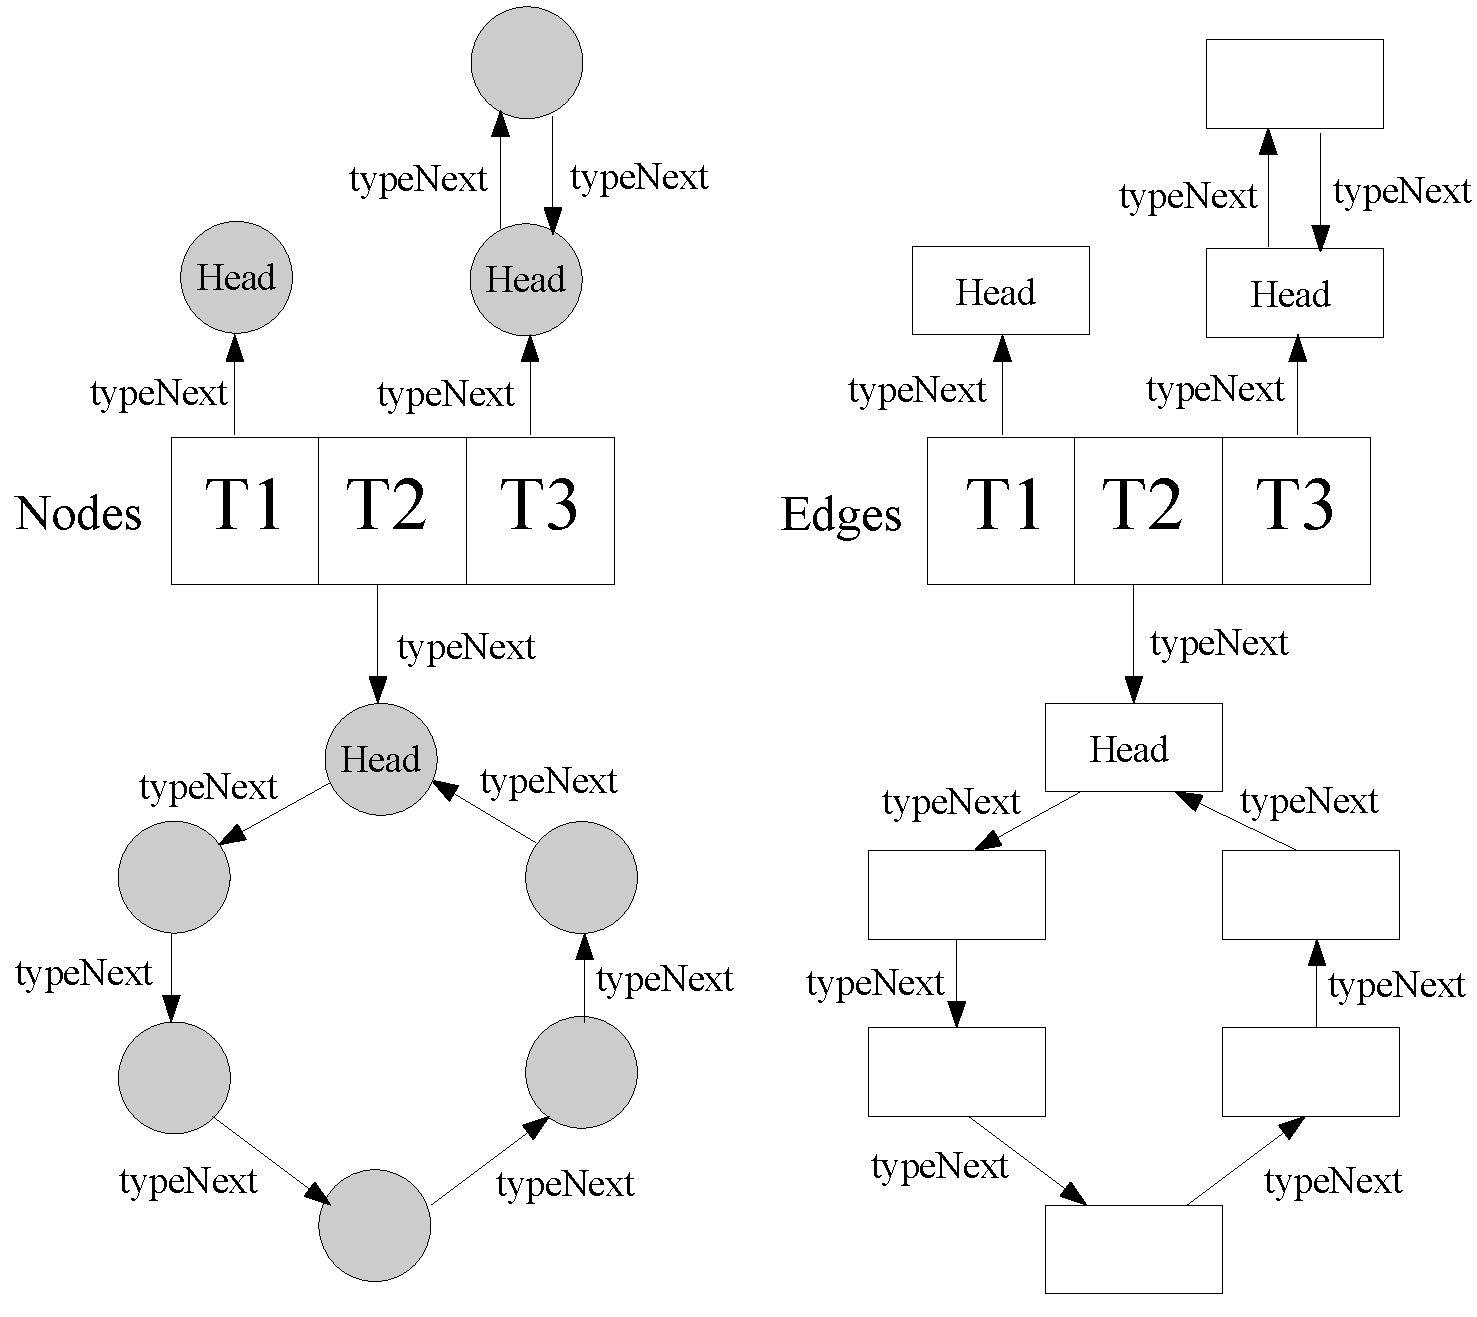
\includegraphics[width=0.65\textwidth]{fig/TypeRinglists}
  \caption{Example for type ringlists}
  \label{figtyperinglists}
\end{figure}

The connectedness information is also stored in ringlists, two ringlists per node object,
one containing the incoming edges and one containing the outgoing edges.
The node object contains a field \texttt{inHead} referencing an arbitrary edge object of the incoming edges (or \texttt{null} of there is none) and a field \texttt{outHead} referencing an arbitrary edge object of the outgoing edges (or \texttt{null} if there is none).
These lists allow to quickly retrieve all incoming or all outgoing edges of a node.

The edge objects contain fields \texttt{source} and \texttt{target} referencing the source and the target node.
They give instant access to the source and target nodes of an edge.
Furthermore, edges contain a field \texttt{inNext} referencing the next edge in the incoming ringlist they are contained in, and a field \texttt{outNext} referencing the next edge in the outgoing ringlist they are contained in.

All the 3 ringlists (type, in, out) are doubly linked to allow for fast insertion and deletion.
For every \texttt{next} field there is also a \texttt{prev} field available that references the previous element in the ringlist (\texttt{typePrev}, \texttt{inPrev}, \texttt{outPrev}).
The figure \ref{figincidenceexampleringlists} gives the ringlist implementation of the example graph depicted in figure \ref{figincidenceexample}. 

\begin{figure}[htbp]
  \centering
  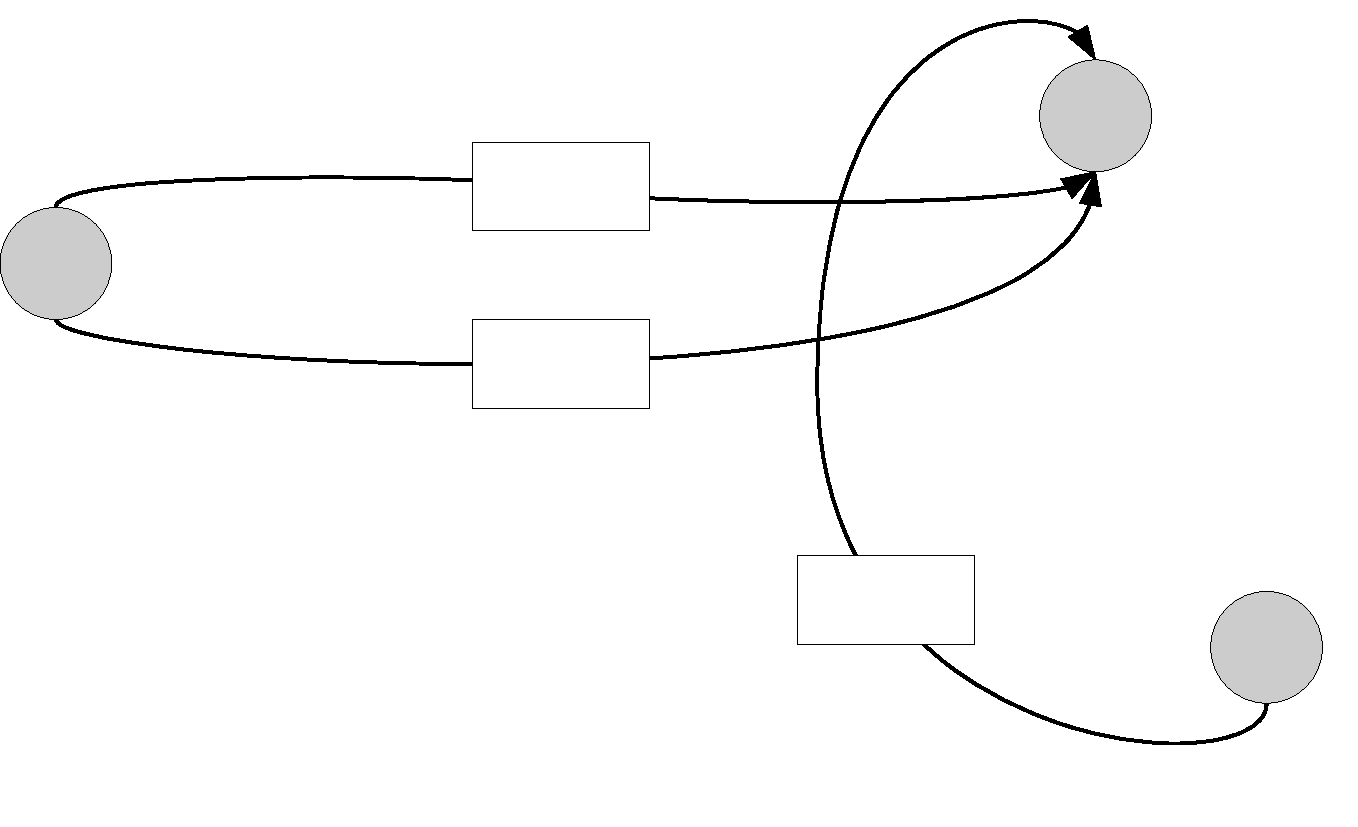
\includegraphics[width=0.75\textwidth]{fig/IncidenceExample}
  \caption{Incidence example situation}
  \label{figincidenceexample}
\end{figure}

\begin{figure}[htbp]
  \centering
  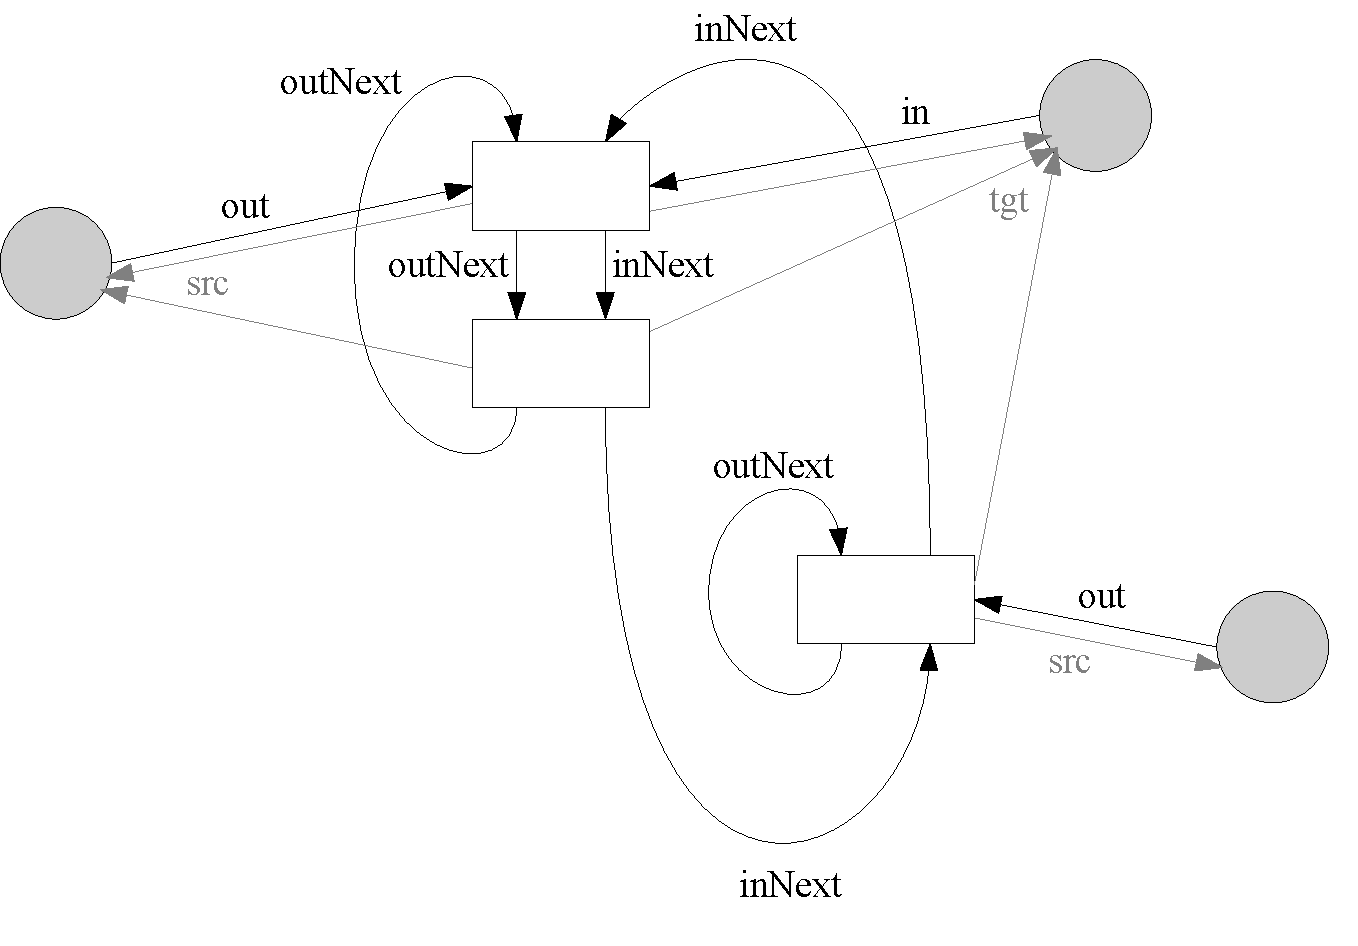
\includegraphics[width=0.75\textwidth]{fig/IncidenceExampleRinglists}
  \caption{Ringlist implementation of incidence example}
  \label{figincidenceexampleringlists}
\end{figure}

In case attribute indices were declared, a balanced search tree (an AA-tree) is created for each of them.
The tree is maintained by event handlers that listen to graph element creation and deletion, but esp. for attribute assignment.

Naming is implemented by the \texttt{LGSPNamedGraph}, the uniqueness constraints/the index by the \texttt{LGSPUniquenessEnsurer}/\texttt{LGSPUniquenessIndex}.
The \texttt{LGSPGraphStatistics} class stores the graph analyzation results (element count and vstruct statistics).

\subsection*{Pattern Matching and Search Programs}\indexmain{pattern matching implementation}\indexmain{search program}

The pattern of an action (rule or test) is matched with a backtracking algorithm that is binding one pattern element after another to a graph element, while checking if it fits to the already bound parts. 
If it does fit, search continues trying to bind the next pattern element, 
or succeeds in case the last check succeeded, building the match object from all the elements bound.
If it does not fit, search continues with the next graph element candidate for the pattern element.
If all graph element candidates for this pattern element are exhausted, search backtracks to the previous decision point and continues there with the next graph element candidate, or fails in case the first check failed.

For every pattern that is to be matched, a search program implementing this algorithm is generated, basically consisting of nested loops iterating the available graph element candidates for each pattern element, and condition checking code that continues search with the next graph element candidate in case of a failing check.
Figure \ref{figpatterntosearchfirst} shows a pattern and a search program generated for it.

\begin{figure}[htbp]
  \centering
  \includegraphics[width=0.7\textwidth]{fig/Pattern}
  \caption{Pattern to search}
  \label{figpatterntosearchfirst}
\end{figure}

\begin{csharp}
foreach(v1:A in graph) {
	foreach(e1 in outgoing(v1)) {
		if(type(e1)!=a) continue;
		v2 = e1.tgt;
		if(type(v2)!=B) continue;
		foreach(e3 in outgoing(v2)) {
			if(type(e3)!=b) continue;
			v3 = e3.tgt;
			if(type(v3)!=C) continue;
			foreach(e2 in outgoing(v3)) {
				if(type(e2)!=a) continue;
				if(e2.tgt!=v2) continue;
				// v1,e1,v2,e3,v3,v2 constitute a match
			} 
		}
	}
}
\end{csharp}

\pagebreak

\subsection*{Search Programs Refined And Rewriting} %kraut und rüben

If a non-leaf-type (regarding the inheritance hierarchy) is to be matched with a graph \emph{lookup} (the outermost loop in the example, defining the root element for pattern matching), then an additional loop is used that is iterating all the subtypes of the type of the pattern element.
After an initial lookup, search normally follows the pattern structure (matching it against graph structure), by iterating the \emph{incoming} or \emph{outgoing} edges of a node, or determining the \emph{source} or \emph{target} node of an edge.
If a pattern is given one or more parameters, search normally continues from the parameters on, picking those as roots, instead of looking up by type in the graph.
If a pattern consists of several unconnected components, several lookups are needed.

Undirected or arbitrarily directed pattern edges are searched in both ringlists, the ringlist of the incoming and the ringlist of the outgoing edges (undirected edge types are otherwise implemented like directed edge types).
Other matching operations besides graph lookup and incoming/outgoing or source/target following are storage access, storage attribute access and storage mapping.
The condition checking code may be targeted at different constraints:
a graph element candidate may get rejected because of its type, missing structural connections to already bound elements, or because the graph element is already matched to another pattern element (isomorphy checking).
Furthermore, attribute conditions may have to be checked, negative patterns for non-matches, and independent patterns for matches (these conditions are normally depending on multiple elements).

Compared with pattern matching, a search task that may need a long time, pattern rewriting is a simple task that executes quickly. 
It consists of a sequence of operations, most notably: i) new nodes creation, then new edge creation, ii) attribute evaluation and assignment, iii) edge deletion, then node deletion, iv) embedded sequences execution (see table \ref{table:executionorderrewriting} for more on this).

A notable performance optimization allowed by the graph model is \indexed{search state space stepping}: after a pattern was matched, the list heads of the type ringlists, the incoming ringlists and the outgoing ringlists are moved to the position of the matched entries with \texttt{MoveHeadAfter}, \texttt{MoveInHeadAfter} and \texttt{MoveOutHeadAfter}.
With this optimization, the pattern matching during an iteration \texttt{r*} will start where the previous iteration step left, saving the cost of iterating again through all the elements that failed in the previous iteration.

\subsection*{Pushdown Machine for Nested and Subpatterns}\indexmain{pushdown machine}\indexmain{stack machine}\label{pushdownmachine}
Every subpattern (as introduced in chapter \ref{cha:sub}) is matched with a search program that is generated from its pattern, in the way introduced in the previous section. 
The interesting part is how the subpatterns get combined, this is carried out with a $2+n$ pushdown machine.

It consists of a call stack, containing the subpattern instances found, an open tasks stack containing the subpatterns to match, and $n$ result stacks containing the (partial) match object trees.
The subpattern instances on the call stack consist of the currently bound elements in the local variables of the stack frame of the search program.
A task denotes the pattern to match, and the parameters where to start; when a subpattern was matched, its contained subpatterns are pushed to the open tasks stack, then the top of the stack gets processed.
For a normal rule application holds $n=1$, while the number of matches is unbound for an all-bracketed rule.
A simulation of this machine, i.e. the matching process of a pattern using subpatterns is shown on the following pages.

Alternatives are handled like a subpattern with several possible patterns that are tried out, the first pattern that is matching is accepted.
Iterateds are handled like subpatterns whose tasks are not removed from the open tasks stack when they get matched, but only if matching failed or the maximum amount of matches was reached.
In case of a failure the minimum required amount of matches is inspected, if the amount of found matches is larger or equal then matching partially succeeds and continues with the next open task (or plain succeeds if there are no open tasks left), otherwise matching of the given partial match fails, causing matching to backtrack (to the previous decision point).

The advantages of this design linearizing the pattern tree on the call stack are the rather low usage of heap memory, the ability to reuse the matcher programs for the patterns as introduced in the previous section, and the ability to find all matches (the $n$ in $2+n$ pushdown machine stands for the number of matches found).

Rewriting is carried out by a depth-first traversal of the match object tree, creating new elements before descending, evaluating attributes and deleting old elements before ascending. 
For each pattern piece matched, the modification specified in the rewrite part is carried out, i.e. the overall rewrite gets combined from the rewrites of the pattern pieces (cf. table \ref{table:executionorderrewriting} for the order of rewriting).

The subpattern usage parameters are computed during matching from matched elements and call expressions (inherited attribution), LHS yielding is carried out after the match was found during match object building with the yield statements (synthesized attribution), RHS yielding is carried out during match object tree rewriting with the eval statements (left attribution, with a user defined left-relation).

In the following, an example run of the $2+n$ pushdown machine is given:

\vspace{16cm} % manual layout so the pushdown simulation starts on its own page

\begin{figure}[htbp]
  \centering
  \includegraphics[width=\textwidth]{fig/Passungszustand1}
  \caption{1. Start state}
  \label{figmatchingstate1}
\end{figure}

\begin{figure}[htbp]
  \centering
  \includegraphics[width=\textwidth]{fig/Passungszustand2}
  \caption{2. The terminal part of pattern A was matched}
  \label{figmatchingstate2}
\end{figure}

\begin{figure}[htbp]
  \centering
  \includegraphics[width=\textwidth]{fig/Passungszustand3}
  \caption{3. The tasks for subpatterns B and C are pushed}
  \label{figmatchingstate3}
\end{figure}

\begin{figure}[htbp]
  \centering
  \includegraphics[width=\textwidth]{fig/Passungszustand4}
  \caption{4. The task for B gets executed, the terminal part of B was matched}
  \label{figmatchingstate4}
\end{figure}

\begin{figure}[htbp]
  \centering
  \includegraphics[width=\textwidth]{fig/Passungszustand5}
  \caption{5. The task for alternative D is pushed}
  \label{figmatchingstate5}
\end{figure}

\begin{figure}[htbp]
  \centering
  \includegraphics[width=\textwidth]{fig/Passungszustand6}
  \caption{6. The task for D gets executed, D1 is tried, but matching fails}
  \label{figmatchingstate6}
\end{figure}

\begin{figure}[htbp]
  \centering
  \includegraphics[width=\textwidth]{fig/Passungszustand7}
  \caption{7. The task for D gets executed, D2 was matched}
  \label{figmatchingstate7}
\end{figure}

\begin{figure}[htbp]
  \centering
  \includegraphics[width=\textwidth]{fig/Passungszustand8}
  \caption{8. The task for C gets executed, C was matched, a match for the overall pattern was found, but is contained only on the call stack}
  \label{figmatchingstate8}
\end{figure}

\begin{figure}[htbp]
  \centering
  \includegraphics[width=\textwidth]{fig/Passungszustand9}
  \caption{9. The match of C is popped from the call stack and pushed to the result stack}
  \label{figmatchingstate9}
\end{figure}

\begin{figure}[htbp]
  \centering
  \includegraphics[width=\textwidth]{fig/Passungszustand10}
  \caption{10. The match of D2 is popped from the call stack and pushed to the result stack}
  \label{figmatchingstate10}
\end{figure}

\begin{figure}[htbp]
  \centering
  \includegraphics[width=\textwidth]{fig/Passungszustand11}
  \caption{11. The match of B is popped from the call stack, D2 from the result stack is added, the combined match is pushed to the result stack}
  \label{figmatchingstate11}
\end{figure}

\begin{figure}[htbp]
  \centering
  \includegraphics[width=\textwidth]{fig/Passungszustand12}
  \caption{12. The match of A is popped from the call stack, B and C from the result stack are added, now we got the combined match of the overall pattern}
  \label{figmatchingstate12}
\end{figure}


% belongs logically to following section
\begin{figure}[htbp]
  \centering
  \includegraphics[width=0.7\textwidth]{fig/Pattern}
  \caption{Pattern to search}
  \label{figpatterntosearch}
\end{figure}

\begin{figure}[htbp]
  \centering
  \includegraphics[width=0.7\textwidth]{fig/Graph}
  \caption{Host graph to search in}
  \label{figgraphtosearchin}
\end{figure}


%%%%%%%%%%%%%%%%%%%%%%%%%%%%%%%%%%%%%%%%%%%%%%%%%%%%%%%%%%%%%%%%%%%%%%%%%%%%%%%%%%%%%%%%%%%%%%%%
\section{Search Planning in Code Generation}\indexmain{search plan}\indexmain{schedule}\indexmain{arborescence}\indexmain{search program}
\indexmain{host graph sensitive search plan driven graph pattern matching}\label{searchplanning}

In the previous section, a search program for the pattern repeated in figure \ref{figpatterntosearch} was given.
It follows the schedule\\
\texttt{lkp(v1:A); out(v1,e1:a); tgt(e1,v2:B); out(v2,e3:b); tgt(e3,v3:C); out(v3,e2:a)}

A \emph{schedule} is a more abstract version of a search program, consisting of a list of search operations.
Available are the search operations \texttt{lkp}, denoting node (or edge) lookup in the graph by iterating the type list, 
\texttt{out} iterating the outgoing edges of the given source node and \texttt{in} iterating the incoming edges of the given target node,
as well as \texttt{src} fetching the source node from the given edge and \texttt{tgt} fetching the target node from the given edge.

The schedule might work well for some graphs, but for the graph given in figure \ref{figgraphtosearchin} it is a bad schedule.
Why so can be seen on inspecting the search order illustration in figure \ref{figbadsearch}.
Because only one of the multiple outgoing edges of \texttt{v1} leads to a match for \texttt{e1}, it has to backtrack several times.
A better search order would be one matching edge \texttt{e1} from \texttt{v2} on in reverse direction 
(this is possible in \GrG\~ because the graph model contains a list of outgoing as well as a list of incoming edges, so each edge can be traversed in either direction).

And indeed, the search planning component of \GrG~chooses such a schedule:\\
\texttt{lkp(v3:C); out(v3,e2:a); tgt(e2,v2:B); out(v2,e3:b); in(v2,e1:a); src(e1,v1:A)}

It leads to the search order depicted in figure \ref{figgoodsearch}, and the search program:

\begin{csharp}
foreach(v3:C in graph) {
	foreach(e2 in outgoing(v3)) {
		if(type(e2)!=a) continue;
		v2 = e2.tgt;
		if(type(v2)!=B) continue;
		foreach(e3 in outgoing(v2)) {
			if(type(e3)!=b) continue;
			if(e3.tgt!=v3) continue;
				foreach(e1 in incoming(v2)) {
				if(type(e1)!=a) continue;
				v1 = e1.src;
				if(type(v1)!=A) continue;
				buildMatchObjectOfPatternWith(v3,e2,v2,e3,e1,v1);
			} 
		}
	}
}
\end{csharp}

\vspace{15cm}

\begin{figure}[hptb]
  \centering
  \includegraphics[width=0.7\textwidth]{fig/GraphBad}
  \caption{Bad search order}
  \label{figbadsearch}
\end{figure}

\begin{figure}[hpbt]
  \centering
  \includegraphics[width=0.7\textwidth]{fig/GraphGood}
  \caption{Good search order}
  \label{figgoodsearch}
\end{figure}

For every pattern, there are normally multiple potential search programs existing,
each capable of finding all the matches, but with vastly different performance characteristics.
In order to improve performance, \GrG~ executes a search planning phase.
With the goal of finding a good schedule, it tries to prevent
\begin{itemize}
	\item following graph structures splitting into breadth as given in this example, or
	\item lookups on types that are available in high quantities.
\end{itemize}

In more detail, the mechanism of search planning works by constructing a \emph{search plan graph} from the pattern graph.
A search plan graph is an edge-weighted graph, with nodes corresponding to the pattern elements -- both nodes and edges -- and edges representing operations to match them, with weight attributes giving an estimated cost of the operation. 
A search plan graph contains an additional root node, with an outgoing edge to each other node defining a \texttt{lookup} operation. 
From plan nodes created for nodes, edges are leading to plan nodes created for edges, denoting \texttt{outgoing} and \texttt{incoming} operations.
From plan nodes created for edges, edges are leading to plan nodes created for nodes, denoting \texttt{source} and \texttt{target} operations.
The cost of the operations is determined by analyzing the amount of splitting between adjacent nodes for every triple of $(node type, edge type, node type)$ in the graph -- called a \indexed{V-Structure} -- and by counting the number of elements of every node type or edge type.

Then, a \emph{spanning arborescence}\footnote{directed tree} of minimum overall cost is selected from the search plan graph. 
The spanning arborescence is further linearized into a \emph{schedule}, a list of the selected search operations  (as already introduced with the good and the bad schedules).

The details of search planning and some evaluation how well it works are given in \cite{Bat:06} and in \cite{BKG:07}.

\begin{figure}[htbp]
  \centering
  \begin{tikzpicture}[bend angle=15]
    \tikzstyle{every node}=[minimum height=0.7cm,minimum width=0.9cm];

    \node[draw,ellipse,fill=white,inner sep=5pt] (root) at (6,0.5) {root};

    \node[draw,ellipse] (v1) at (0,5) {$\mathit{v1:A}$};
    \node[draw] (e1) at (3,5) {$e1:a$};
    \node[draw,ellipse] (v2) at (6,5) {$\mathit{v2:B}$};
    \node[draw] (e2) at (9.75,7) {$e2:a$};
    \node[draw] (e3) at (9.75,3.5) {$e3:b$};
    \node[draw,ellipse] (v3) at (13.5,5) {$\mathit{v3:C}$};

    \draw[-latex,bend left] (root.north) to node[near end, sloped, below] {$\mathsf{lkp}$/2} (v1.south);
    \draw[-latex] (root.north) -- (e1.south) node[near end, sloped, below] {$\mathsf{lkp}$/7};
    \draw[-latex] (root.north) -- (v2.south) node[midway, sloped, below] {$\mathsf{lkp}$/4};
    \draw[-latex,bend right] (root.north) to node[near end, sloped, below] {$\mathsf{lkp}$/7} (e2.south);
    \draw[-latex] (root.north) -- (e3.south) node[near end, sloped, below] {$\mathsf{lkp}$/2};
    \draw[-latex,bend right,line width = 2pt] (root.north) to node[near end, sloped, below] {$\mathsf{lkp}$/1} (v3.south);

    \draw[-latex,bend left] (v1) to node[midway, above] {$\mathsf{out}$/2.83} (e1);
    \draw[-latex,bend left,line width = 2pt] (e1) to node[midway, below] {$\mathsf{src}$/1} (v1);
    \draw[-latex,bend right] (e1) to node[midway, below] {$\mathsf{tgt}$/1} (v2);
    \draw[-latex,bend right,line width = 2pt] (v2) to node[midway, above] {$\mathsf{in}$/1} (e1);
    \draw[-latex,bend left] (v2) to node[midway, above] {$\mathsf{out}$/1} (e2);
    \draw[-latex,bend left,line width = 2pt] (e2) to node[midway, below] {$\mathsf{src}$/1} (v2);
    \draw[-latex,bend left,line width = 2pt] (v2) to node[midway, above] {$\mathsf{out}$/1} (e3);
    \draw[-latex,bend left] (e3) to node[midway, below] {$\mathsf{src}$/1} (v2);
    \draw[-latex,bend right] (e2) to node[midway, below] {$\mathsf{tgt}$/1} (v3);
    \draw[-latex,bend right,line width = 2pt] (v3) to node[midway, above] {$\mathsf{in}$/1} (e2);
    \draw[-latex,bend right] (e3) to node[midway, below] {$\mathsf{tgt}$/1} (v3);
    \draw[-latex,bend right] (v3) to node[midway, above] {$\mathsf{in}$/2} (e3);
  \end{tikzpicture}
  \caption{
  	The search plan graph for the pattern graph of Figure~\ref{figpatterntosearch} with estimated backtracking costs induced by the host graph of Figure~\ref{figgraphtosearchin}.
	The found minimum directed spanning tree is denoted by thick edges.
  }
  \label{fig:plan-graph}
\end{figure}

Afterwards, a search program is constructed from the schedule. 
It is situated at a level of abstraction in between the schedule and the code finally emitted.
Structurally, it is a tree resembling the syntax tree of the code to generate, as sketched in figure \ref{figsearchprogram} (with list entries maybe containing further lists). 

\begin{figure}[htbp]
  \centering
  \includegraphics[width=0.9\textwidth]{fig/SearchProgram}
  \caption{A simple Search Program}
  \label{figsearchprogram}
\end{figure}

It contains explicit instructions for isomorphy checking and connectedness checking (whose are depending on the exact schedule).
Furthermore, it contains exact locations where to continue at; these target search operations may be different from the directly preceding search operation (because that one does not define a choice point of influence).

Connectedness checking can be seen in the search program of the good example in the check that the target of \texttt{e3} is indeed \texttt{v3};
a target matching operation \texttt{tgt(e3,v3:C)} is not used because \texttt{v3} was already matched by the lookup operation, and is already contained in the spanning tree.

A remark on isomorphy checking that ensures that two pattern elements are not bound to the same graph element:
as a consequence of the simple loop-after-loop based assignment of graph elements to pattern elements, the pattern elements would get matched homomorphically to each other by default, 
if an explicit check against would not be inserted (because assignment starts with the same graph elements, the homomorphic matches often \emph{are} the first ones found).
Isomorphy checking is implemented by flags that are contained in the graph elements, and are set when a graph element is bound to a pattern variable, and reset when the binding is given up again 
(one flag for each negative/independent nesting level, until the implementation defined limit of flags available in the graph elements is reached, then a list of dictionaries is used).
The flags are then checked in the following, nested matching operations. 
An iso-check scheduling pass ensures that checks are only inserted if the elements must be isomorphic and their types do not already ensure that they cannot get matched to the same elements.

%%%%%%%%%%%%%%%%%%%%%%%%%%%%%%%%%%%%%%%%%%%%%%%%%%%%%%%%%%%%%%%%%%%%%%%%%%%%%%%%%%%%%%%%%%%%%%%%
\section{The Code Generator}\indexmain{code generator}

\subsection{Frontend}

\begin{figure}[htbp]
  \centering
  \includegraphics[width=\textwidth]{fig/AblaufCodeerzeugungFrontend}
  \caption{Frontend Code Generation}
  \label{figfrontendcodegen}
\end{figure}

The frontend is spread over the directories \texttt{parser}, \texttt{ast}, \texttt{ir}, \texttt{be} and \texttt{util}, with their code being used from \texttt{Main.java}.

\subsubsection*{Syntax and Static Semantics}
The directory \texttt{parser} contains parser helpers like the symbol table and scopes and within the \texttt{antlr} subdirectory the ANTLR parser grammar of \GrG~in the files \texttt{Grgen.g} and \texttt{EmbeddedExec.g}.
The semantic actions of the parser build an abstract syntax tree consisting of instances of the classes given in the directory \texttt{ast}, with the base class \texttt{BaseNode}.
The AST is operated upon in three passes, first resolving by \texttt{resolve} and \texttt{resolveLocal}, mainly replacing identifier nodes by their declaration nodes during a (largely) preorder walk.
Afterwards, the AST is checked by \texttt{check} and \texttt{checkLocal} during a (largely) postorder walk for type and other semantic constraints.
Finally, an intermediate representation is built from the abstract syntax tree by the \texttt{getIR} and \texttt{constructIR} methods.

\subsubsection*{Intermediate Representation}
The IR classes given in the \texttt{ir} folder can be seen as more lightweight AST classes; their name is often the same as for their corresponding AST classes, but without the \texttt{Node}-suffix which is appended to all AST classes.
The most interesting classes are \texttt{Rule} used for rules, alternative cases and iterateds, as well as \texttt{PatternGraphLhs} used for all left hand side pattern graphs including negatives and independents, and \texttt{PatternGraphRhs} used for all right hand side pattern graphs;
several data flow analyses are contained in \texttt{PatternGraphLhs}, some covering the nesting of patterns, some being even global.

A particularly interesting one is \texttt{ensure\-Directly\-Nesting\-Pattern\-Contains\-All\-Non\-Local\-Elements\-Of\-Nested\-Pattern}, it ensures that, from a pattern which contains a certain entity the first time, up to every pattern that references this entity, all intermediate patterns contain that entity, too.
It is implemented with a recursive walk over the nested patterns in the IR-structure. 
Each pattern receives the set of already known elements as parameter.
Before descending, the elements available in the current pattern are added to the set of already known elements,
then recursive descent into the directly nested patterns follows, handing down the already known elements.
On ascending, elements are added to the current pattern if they are contained in a directly nested pattern, but not in the current pattern, although they are known in the current pattern.
This function allows keep the backends simple.

The IR classes are the input to the two backends of the JAVA frontend.
They can be found in the folders \texttt{be/C} and \texttt{be/Csharp}.


\subsubsection*{Backends}

The directory \texttt{be/C} contains the code generator for the C based backend, which is integrated into the IPD C compiler.
(The compiler transforms a C program into a graph and SSA based compiler intermediate representation named FIRM using libFirm (see \url{libfirm.org}, \cite{TBL:99}, \cite{Lin:02}) and further on to x86 machine code.)

The directory \texttt{be/Csharp} contains the code generator for the C\# based backend of \GrG. 
It generates the source code for the model with the node and edge classes, in \texttt{FooModel.cs} for a rule file named \texttt{Foo.grg},
and the intermediate source code for the rules, consisting of a specification of the patterns to match, a listing of the embedded graph rewrite sequences, and the rewriting code, in \texttt{Foo\-Actions\_intermediate.cs}.
This is done in several recursive passes over the nesting structure of the patterns in the IR. 

The backend of the frontend does \emph{not} generate the complete source code for the rules including the matcher code or the code for the embedded rewrite sequences --- this is done by \texttt{grgen.exe}, which calls the \texttt{grgen.jar} of the frontend.
You may call the Java archive on your own in order to get a visualization of the model and rewrite rules, in the form of a \texttt{.vcg}-dump of the IR, cf. Note\ref{note:modelruledump}.


\subsubsection*{Model Generation}

The model generation code in \texttt{ModelGen} is rather straight forward:
\begin{enumerate}
	\item first, code for the user defined enums is generated,
	\item then the node classes are generated,
	\item followed by the node model,
	\item then the edge classes are generated,
	\item followed by the edge model,
	\item and finally, the graph model is generated.
\end{enumerate}

\noindent For the nodes as well as for the edges, three classes are generated:
\begin{enumerate}
	\item the first is the interface visible to the user, giving access to the attributes,
	\item the second is the implementation of the interface, also inheriting from \texttt{LGSPNode} or \texttt{LGSPEdge},
	\item and the third is a type representation class, which is inheriting from \texttt{NodeType} or \texttt{EdgeType}, that is giving information about the type and its attributes, and is used in the node/edge model and thus the graph model.
\end{enumerate}

Additionally, the indices are generated by \texttt{Model\-Index\-Gen}, and functionality regarding external extensions by \texttt{Model\-External\-Gen}.

\subsubsection*{Rule Representation Pass}

The code -- better representation -- generation of the actions is implemented in \texttt{ActionsGen}, in the code called from \texttt{gen\-Subpattern} for the subpatterns and \texttt{gen\-Action} for the rules and tests.

In a prerun from \texttt{gen\-Rule\-Or\-Subpattern\-Class\-Entities} on, some needed entities are generated, e.g. type arrays for the allowed types of the pattern elements (the arrays are only filled if the base type was constrained), or indexing enums, which map the pattern element names to their index in the arrays of the matched host graph elements in the match objects of the generic match interface.

In the rule representation pass, from \texttt{gen\-Rule\-Or\-Subpattern\-Init} on, the subpattern- and rule representations of type \texttt{Matching\-Pattern} and \texttt{Rule\-Pattern} are generated, including the contained \texttt{Pattern\-Graph}-objects for the (nested) pattern graph(s), by mutually recursive calls of \texttt{gen\-Pattern\-Graph} and \texttt{gen\-Elements\-Required\-By\-Pattern\-Graph}.

The method \texttt{gen\-Elements\-Required\-By\-Pattern\-Graph} generates for a pattern graph its contained elements, the pattern nodes, the pattern edges, the used subpatterns as \texttt{Pattern\-Graph\-Embedding} members, the contained alternatives, and the iterateds; the representations of contained negative subpatterns and alternative cases are generated by \texttt{gen\-Pattern\-Graph} before the containing pattern. 

A graph element contained in a pattern, but defined in a nesting pattern, is saved in the pattern as a reference to the element in the nesting pattern. 
The \texttt{Pattern\-Graph} in which it was used first is remembered in a \texttt{Point\-Of\-Definition} member variable.
The source and target nodes of edges are saved in the \texttt{Pattern\-Graph} in hash tables (so that an edge with an undefined source or target can be refined in a nested pattern); source and target nodes are determined by ascending alongside the pattern nesting until a definition is found.

As all graph elements, including the ones of the nested patterns, are created flatly in the \texttt{initialize}-method of the \texttt{Matching\-Pattern}, name prefixes are needed to prevent name clashes; this is ensured by the parameter \texttt{path\-Prefix}.
Correct naming of already declared elements is ensured with a \texttt{already\-Defined\-Entity\-To\-Name}-hash-table.
The split into constructor and \texttt{initialize} method is needed because a recursive \texttt{Matching\-Pattern} must reference itself at construction.

Furthermore, local and global homomorphy tables for the nodes and the edges are generated, defining which pattern elements are allowed to match the same host graph element (the global tables specify the homomorphy in between elements from the \texttt{Pattern\-Graph} of an alternative case or an iterated, and an enclosing \texttt{Pattern\-Graph}).

Additionally, expression trees for the attribute checks and statement blocks for the yieldings are generated, by \texttt{ActionsExpressionOrYieldingGen}.

Finally (the exact) match classes are generated by \texttt{Actions\-Match\-Gen}, for every pattern besides negative patterns an interface and a class implementing this interface.
The match classes are instantiated after a match of the corresponding pattern was found, giving a highly convenient and type safe interface to the matched entities at API level.

For embedded sequences, representations in form of \texttt{LGSP\-Embedded\-Sequence\-Info} objects are generated, which contain the sequence as string, plus additional parameter information; the real sequence code is generated in the backend.
For sequences embedded in alternatives, iterateds, or subpatterns, additionally closure classes inheriting from \texttt{LGSP\-Embedded\-Sequence\-Closure} are generated.
They store the graph elements the pattern elements from the pattern containing the exec were bound to; the sequence execution function is then called on this closure, which is stored in a queue, and executed from the top level rule.
All of this is carried out in \texttt{ActionsExecGen}.

\subsubsection*{Rewrite Code Pass}
In the rewrite pass, the rewrite code gets generated, via \texttt{gen\-Modify} of \texttt{Modify\-Gen}.
The nesting of negative or independent patterns does not need to be taken care of here, as they come without rewrite parts.

For every pattern piece and its rewrite role (dependent rewriting, creation, deletion) are local rewrite methods generated, carrying out the complete rewriting by calling each other at runtime.
\texttt{Modify\-Generation\-State} holds the state during generation, while the \texttt{Modify\-Generation\-Task}s allow to give a left and right graph independent of the rewriting specified with the rule (so the creation and deletion code can be generated in addition to the dependent rewrite).
The code for subpattern creation is generated by using an empty graph as left graph and the pattern graph as right graph.
The code for subpattern deletion is generated by using the pattern graph as left graph and an empty graph as right graph.
The code for dependent rewriting is generated by simply referencing the graphs from \texttt{IR::Rule}.
For a test, the pattern graph is used as left and right graph.
For alternatives and iterateds, dispatching methods are generated, calling the rewrite methods of the instances of the patterns matched.
Rewrite parameters are mapped to local parameters of the rewrite methods.

The core method of rewrite code generation named \texttt{gen\-Modify\-Rule\-Or\-Subrule} generates the rewriting of the given pattern and the calls to the rewrite methods of the nested patterns.
The rewrite methods of the nested patterns are prefixed with their nesting path, in order to avoid name conflicts, which may occur as they are placed flatly in their \texttt{Matching\-Pattern} or \texttt{Rule\-Pattern}.
Their role is distinguished by one of the name postfixes \texttt{Modify}, \texttt{Create} or \texttt{Delete}; for keeping a pattern unmodified obviously no methods are needed.

Also during the rewrite pass, the statements of the \texttt{eval} blocks are generated, this happens in \texttt{Modify\-Eval\-Gen}, and the calls of the routines implementing the embedded \texttt{exec}s, in \texttt{Modify\-Exec\-Gen}.

\pagebreak

\subsection{Backend}

The real matcher code is generated by the backend given in \texttt{engine-net-2}, in the \texttt{src/lgsp\-Backend} subdirectory.
The generation is carried out in several passes in, or better from \texttt{lgsp\-Matcher\-Generator.cs} on.
The base data structure is the \texttt{PatternGraph}, resp. the nesting of the \texttt{PatternGraph}-objects, contained in the \texttt{RulePattern}-objects of the rules/tests or the \texttt{Matching\-Pattern}-objects of the subpatterns.

\subsubsection*{1. Step}

\begin{figure}[htbp]
  \centering
  \includegraphics[width=\textwidth]{fig/AblaufCodeerzeugungBackend1}
  \caption{Backend Code Generation, step 1}
  \label{figbackendcodegen1}
\end{figure}

First, the subpattern usages are inlined when \indexed{inlining} is assumed to be beneficial.
(This allows you to extract common patterns into subpatterns increasing readability and modularity without loosing performance (but as of now only one level of inlining is supported, so beware of too much subpattern extraction, especially if the containing pattern would get disconnected by this)). 
After (and partly before) this kind of pattern rewriting, the patterns and their relations are analyzed by the \texttt{PatternGraphAnalyzer} -- the analyzation results are used for emitting better code later on (choosing more efficient but more limited implementations of language features, which are not sufficient in the general case but are so for the specification at hand).
Then a \texttt{PlanGraph} is created from the \texttt{PatternGraph} and data from analyzing the host graph (for generating the initial matcher some default data from the frontend is used).
A minimum spanning arborescence is computed defining a hopefully optimal set of operations for matching the pattern (the hopes are founded, see \cite{BKG:07}).
A \texttt{SearchPlanGraph} is built from the arborescence marked in the \texttt{PlanGraph} and used thereafter for scheduling the operations into a \texttt{ScheduledSearchPlan}, which gets completed by \texttt{Append\-Homomorphy\-Information} with isomorphy checking information.
The \texttt{ScheduledSearchPlan} is then stored in the \texttt{PatternGraph} it was computed from.


\subsubsection*{2. Step}

\begin{figure}[htbp]
  \centering
  \includegraphics[width=0.5\textwidth]{fig/AblaufCodeerzeugungBackend2}
  \caption{Backend Code Generation, step 2}
  \label{figbackendcodegen2}
\end{figure}

In a second step, the \texttt{Schedules} of the negative or independent \texttt{Pattern\-Graph}s are integrated into the \texttt{Schedule} of the enclosing \texttt{Pattern\-Graph}, by \texttt{Merge\-Negative\-And\-Independent\-Schedules\-Into\-Enclosing\-Schedules} (in the \texttt{Schedule\-Enricher}-class), in a recursive run over the nesting structure of the \texttt{Pattern\-Graph}s in the \texttt{Matching\-Pattern}s or \texttt{Rule\-Pattern}s.
Due to nested negative or independent graphs, this may happen spanning several nesting levels;
the result is saved in the \texttt{Schedule\-Including\-Negatives\-And\-Independents} field of the non-negative/independent \texttt{Pattern\-Graph}s.


\subsubsection*{3. Step}

\begin{figure}[htbp]
  \centering
  \includegraphics[width=\textwidth]{fig/AblaufCodeerzeugungBackend3}
  \caption{Backend Code Generation, step 3}
  \label{figbackendcodegen3}
\end{figure}

Finally, in a third step, code is generated by \texttt{Generate\-Action\-And\-Matcher},
again in a recursive run over the nesting structure of the \texttt{Pattern\-Graph}s, 
using the \texttt{Schedule\-Including\-Negatives\-And\-Independents} stored in them. 

For each \texttt{Rule\-Pattern}, an \texttt{Action}-class is generated, 
and for each \texttt{Matching\-Pattern}, a \texttt{Subpattern\-Action}-class is generated.
Additionally, for each alternative an \texttt{Alternative\-Action}-class is generated,
the alternative matcher will contain code for all alternative cases.
For each iterated, an \texttt{Iterated\-Action}-class is generated.
The real matching code is then generated into these classes.

The \texttt{Search\-Program\-Builder} builds a \texttt{Search\-Program} tree data structure resembling the syntax tree of the code to generate out of the \texttt{Schedule\-Including\-Negatives\-And\-Independents} in the \texttt{Pattern\-Graph}s. 
To be more precise: the \texttt{Search\-Program\-Builder} builds the \texttt{Search\-Program} matcher routine heads and then employs a \texttt{Search\-Program\-Body\-Builder} to build the bodies of the matcher routines -- consisting of diverse \texttt{Search\-Program\-Operation}s -- in a run over the schedule with \texttt{Build\-Scheduled\-Search\-Plan\-Operation\-Into\-Search\-Program}, one input \texttt{Search\-Operation} after the other. 
In a further pass, the \texttt{Search\-Program} is completed by the \texttt{Search\-Program\-Completer},
determining the locations to continue at when a check fails,
writing undo code for the effects which were applied from that point on to the current one.
Finally, the C\# code gets generated by calling the \texttt{Emit} methods of the \texttt{Search\-Program}.
If you want to extend this code, you may be interested in the \texttt{Dump} methods which dump the \texttt{Search\-Program} in an easier readable form into text files.

Besides this pattern-matching related core functionality of \GrG, do you find in the \texttt{lgsp\-Backend/Expression\-Or\-Yielding} folder the classes emitting the code for the condition expressions and yielding statements.
The generated code typically calls one of the helper method available in one of the \texttt{XXXHelper.cs} files in the \texttt{libGr} folder (defining the runtime library for the \GrG-languages).

\subsubsection*{Nested and Subpattern Matching}

The \texttt{Subpattern\-Action}-classes (cf. \ref{figbackendcodegen3}) do not only contain the matcher code, 
but are at the same time the tasks of the $2+n$ pushdown machine, which are pushed on the open tasks stack;
they contain the subpattern parameters as member variables.
The same holds for the \texttt{Alternative\-Action}- and \texttt{Iterated\-Action}-classes,
which do not hold parameters but entities from the nesting pattern they reference. 

The higher levels of code generation are in large parts independent of nested and subpattern matching and control of the $2+n$ pushdown machine.
Only on the level of search programs does it become visible,  
with an \texttt{Initialize\-Subpattern\-Matching}-search program operation at the begin of a search program
and a \texttt{Finalize\-Subpattern\-Matching}-search program operation at the end of a search program;
but mainly with a call to \texttt{build\-Match\-Complete} when the end of the schedule is reached during search program building.
This corresponds to the innermost location in the search program,
the location at which the local pattern was just found (during execution);
now the control code is inserted by \texttt{insert\-Push\-Subpattern\-Tasks},
pushing the tasks for the subpatterns used from this pattern, as well as alternatives and iterateds nested in this pattern.
To execute the open tasks a \texttt{Match\-Subpatterns} operation is inserted into the search program. 
Afterwards, \texttt{insert\-Pop\-Subpattern\-Tasks} inserts the operations for cleaning the task stack,
\texttt{insert\-Check\-For\-Subpatterns\-Found} the operations to handle success and failure, 
and \texttt{insert\-Match\-Object\-Building} the code for maintaining the result stack.


\subsubsection*{libGr and lgspBackend}

The \texttt{src/libGr} subdirectory contains the libGr, offering the base interfaces you see on the API level for the model, the actions, the pattern graphs and the host graph.
The interfaces are implemented by code from the libGr search plan (lgsp) backend in \texttt{src/lgspBackend} and by the generated code.
The generated code defines a type-safe interface of named and typed entities, which is more convenient to use at API level, but bound to a specification.
The libGr in contrast offers a "generic", name string and object or root type based interface.

In addition, it offers the graph rewrite sequence parser, which gets generated from \texttt{Sequence\-Parser.csc},
and is building a graph rewrite sequence AST out of a sequence string, from the classes in \texttt{Sequence.cs}, further utilizing a \texttt{Symbol\-Table} and the \texttt{Sequence\-Parser\-Environment}.
After building, the sequence AST is type checked by the \texttt{Sequence\-Checking\-Environment}, which -- like the parser environment -- comes in a version for the interpreted sequences and a version for the compiled sequences, abstracting away the differences in available (type) information while generating the action code (compiled) compared to using the generated action code (interpreted).

The graph rewrite sequence classes contain a method \texttt{ApplyImpl(IGraph graph)}, which is called at runtime of the transformation for executing the sequence.
The compiled graph rewrite sequences instead get emitted as source code by the \texttt{lgsp\-Sequence\-Generator}.
The \texttt{lgsp\-Sequence\-Generator} works as driver, employing esp. the \texttt{Sequence\-Generator} for generating the rule controlling sequences, which in turn employs esp. the \texttt{Sequence\-Computation\-Generator} for generating the sequence computations, and the \texttt{Sequence\-Expression\-Generator} for generating the sequence expressions.

When GrGen rules are matched, as well as when the graph is changed, events are fired.
They allow to display the matches and graph changes in the debugger,
to record changes to a file for later playback, or record changes to a transaction undo log for later rollback.
You can register event handlers to them, in order to execute your own code (allowing you to build an event based graph rewriting mechanism on API level).
The graph delegates fired are given in \texttt{IGraph.cs}.
Graph events recording is implemented in \texttt{Recorder.cs}, replaying amounts to a normal \texttt{.grs} execution.
Graph transaction handling is implemented in \texttt{lgspTransactionManager.cs}, with a list of undo items, which know how to undo the effect that created them.
They are purged on commit or executed on rollback.
Backtracking is implemented with nested transactions.
If you are changing the graph programmatically at API level (not using GrGen rules), you have to fire some of the events (esp. the ones for attribute assignment) on your own in case you want to use any of the mechanisms (graphical debugging, record and replay, transactions and backtracking, event based programming) above.

The runtime library \texttt{libGr} further contains the interface \texttt{IGraphProcessingEnvironment} to the graph processing environment (built up from a series of environment interfaces with increasing functionality), offering e.g. graph global variables, sequence execution, convenient action execution, as well as graph change recording and transaction handling (implemented by the aforementioned classes in the \texttt{lgspBackend}).
Additionally, it implements helper code in \texttt{XXXHelper.cs} files.

The \texttt{ContainerHelper.cs} contains code that is common for all container types (cf. Chapter~\ref{cha:container}), the \texttt{DictionaryHelper.cs} contains code that is common for sets and maps, while the \texttt{SequentialTypeHelper.cs} contains code that is common for array and deques; code specific to each container type is available in correspondingly named files.
The \texttt{GraphHelper.cs} contains code that implements the diverse graph query functions and graph manipulation procedures (cf. Chapter~\ref{cha:graph}), while the \texttt{GraphHelperParallel.cs} contains code that implements the diverse graph query functions in versions that can be employed from parallelized pattern matchers (which are not allowed to use the isomorphy checking flags contained in the graph elements that are employed by the non-parallel pattern matchers).
The \texttt{Emit\-Helper.cs}, \texttt{Attribute\-Type\-Emit\-Helper.cs} and \texttt{Attribute\-Change\-Type\-Emit\-Helper.cs} contain code for uniform emitting/to-string-conversion of the diverse types supported by \GrG, the \texttt{GrGen\-Types\-Helper.cs}, \texttt{Dot\-Net\-Types\-Helper.cs}, and \texttt{Types\-Helper.cs} files contain type querying and type representation conversion functions (predominantly for internal use).

The \texttt{libGr} offers also several importers and exporters in the \texttt{src/libGr/IO} subfolder, as well as dumpers into file formats meant for visualization.

For graph comparison, a pattern may be created out of one of the graphs, and searched in the other one, by utilizing an \texttt{Interpretation\-Plan\-Builder} to build an \texttt{Interpretation\-Plan}, and by calling \texttt{Execute} on it (an interpretation plan is a simplified version of a search plan, that is executed at runtime instead of getting emitted into an actions file -- when it is utilized a certain number of times, it gets emitted and compiled (at runtime) in order to speed up pattern matching and thus graph comparison.
Take a look at \texttt{lgspBackend/Graph\-Comparison} for the code and at Section~\ref{sec:relationalgraph}) for further explanations.

The filter implementations of the auto-generated filters are generated by the \texttt{Filter\-Generator.cs}, the auto filter for filtering symmetric matches from automorphic patterns is further utilizing the \texttt{Symmetry\-Checker.cs}.
The auto-supplied filters are available pre-implemented in the \texttt{libGr/matches\-Helper.cs} and the \texttt{lgsp\-Backend/Actions/lgsp\-Matches.cs} files.

\subsubsection*{GrShell and Debugger}

The \texttt{src/GrShell} subdirectory contains the GrShell application, which builds upon the sequence interpretation facilities offered by libGr, and the "generic" interface of libGr, because it has to be capable of coping with arbitrary used defined models and actions at runtime.
The command line parser of GrShell gets generated out of \texttt{GrShell.csc}, the shell implementation is given in \texttt{GrShellImpl.cs}, execution starts in the \texttt{Main} method in \texttt{GrShell\-Driver.cs}, and sequence execution is supported by the \texttt{GrShell\-Sequence\-Applier\-And\-Debugger.cs}.
Graphical debugging is offered by the \texttt{Debugger.cs} and several helper classes, esp. including the \texttt{YCompClient.cs}, which implements the protocol available for controlling yComp, communicating with yComp over a tcp connection to localhost.

\subsubsection*{Further Things}

The \texttt{src/GrGen} subdirectory contains the driver procedure of the \texttt{grgen.exe} compiler.

The \texttt{examples} subdirectory of \texttt{engine-net-2} contains a bunch of examples for using \GrG~with GrShell.
The \texttt{examples-api} subdirectory contains several examples of how to use \GrG~from the API.

In case you want to contribute and got further questions don't hesitate to contact us 
(via email to \texttt{grgen} at the host given by \texttt{ipd.info.uni-karlsruhe.de}).




\appendix

\bibliographystyle{alpha}
\bibliography{diss}

\printindex

\end{document}



